%
%
\documentclass[a4paper,pagesize=dvips,onecolumn,11pt,titlepage,twoside]{scrartcl}
% \documentclass[a4paper,dvips,onecolumn,11pt,titlepage]{scrreprt}
\usepackage{qgis_style}


\begin{document}

%  !TeX  root  =  user_guide.tex

\begin{titlepage}
%\addcontentsline{toc}{section}{Titre}
\begin{center}

%\begin{figure}[H]
\begin{center}

\includegraphics{qgislogo} 
\end{center}
%\end{figure}

\Huge{Quantum GIS}\\
\vspace{0.5cm}
\Large{User Guide} \\
\vspace{0.5cm}
%
\includegraphics[clip=true, scale=0.4]{splash} 
\Large{Version ~\CURRENT \textsl{'This is no moon !'}}

\end{center}
\end{titlepage}

%  !TeX  root  =  user_guide.tex
\frontmatter
\pagestyle{scrplain}
\addchap{Préambule}
\vspace{1cm}
Ce document est le manuel officiel d'utilisation du logiciel \QG. Les logiciels et le matériel décrits dans ce document sont pour la plupart des marques déposées et donc soumises à des obligations légales. \QG est distribué sous la Licence publique générale GNU (GPL). Vous trouverez plus d'informations sur la page internet de \QG \url{http://qgis.osgeo.org}.
\par\bigskip
Les détails, données, résultats, etc. inclus dans ce document ont été écrits et vérifiés au mieux des connaissances des auteurs et des éditeurs. Néanmoins, des erreurs dans le contenu sont possibles.
\par\bigskip
Ainsi l'ensemble des données ne saurait faire l'objet d'une garantie. Les auteurs et les éditeurs ne sauraient être responsables de tout dommage direct, indirect, secondaire ou accessoire découlant de l'utilisation de ce manuel. Les éventuelles corrections sont toujours les bienvenues.
\par\bigskip
Ce document a été rédigé avec \LaTeX. Les sources sont disponibles en code \LaTeX{} via\\ \url{https://svn.osgeo.org/qgis/docs/tags/1.3.0_user_guide} et en PDF via \url{http://qgis.osgeo.org/documentation/manuals.html}. 
Des versions traduites peuvent être téléchargées via la section de documentation du projet QGIS. Pour plus d'informations sur les manières de contribuer à ce document et à sa traduction, veuillez visiter \url{http://www.qgis.org/wiki/} 

\vspace{1cm}
\noindent
\textbf{Références de ce document}
\par\bigskip
Ce document contient des références internes et externes sous forme de lien. Cliquer sur un lien interne provoque un déplacement dans le document, tandis que cliquer sur un lien externe ouvrira une adresse internet dans le navigateur par défaut. En PDF, les liens internes seront indiqués en bleu et les externes en rouge. En HTML, le navigateur affiche et gère les deux types de liens de la même fa\c{c}on.

\newpage

\begin{flushleft}
\textbf{Auteurs et éditeurs :}
 \par\bigskip\noindent
\begin{tabular}{p{4cm} p{4cm} p{4cm}}
Tara Athan & Radim Blazek & Godofredo Contreras   \\
 Otto Dassau & Martin Dobias & Claudia A. Engel \\ 
 Carson J.Q. Farmer &J\"urgen E. Fischer & Anne Ghisla \\
Stephan Holl &  Magnus Homann& Marco Hugentobler \\ 
 Lars Luthman & Gavin Macaulay & Werner Macho \\
  Tyler Mitchell & Brendan Morely&Gary E. Sherman\\
  Tim Sutton & David Willis \\ \
\end{tabular}
\end{flushleft}

\begin{flushleft}
\textbf{Traducteurs version francophone:}
  \par\bigskip\noindent
\begin{tabular}{p{4cm} p{4cm} p{4cm}}
Benjamin Bohard & Jeremy Garniaux & Yves Jacolin \\
Stéphane Morel & Jean Roc Morreale & Marie Silvestre \\
Tahir Tamba & Xavier M. & Cyril de Runz \\
Benjamin Lerre \\
\end{tabular}
\end{flushleft}

Nos remerciements vont à Bertrand Masson pour son aide précieuse quant à la mise en page de ce document, Tisham Dhar pour avoir préparé l'environnement initial de documentation pour MS Windows, à Tom Elwertowski et William Kyngesburye pour la section d'installation sur Mac OS X et à Carlos  D\'{a}vila, Paolo Cavallini et Christian Gunning pour les révisions. Si nous avons négligé de citer ici le nom d'un contributeur, veuillez accepter nos excuses pour cet oubli et nous le signaler pour correction.
\par\bigskip\noindent
\textbf{Copyright \copyright~2004 - 2010 \QG Development Team}
\par\bigskip\noindent
\textbf{Internet :} \url{http://qgis.osgeo.org}

\addsec{Licence de ce document}

La permission de copier, distribuer, modifier ce document est accordée sous les termes de la GNU Free Documentation License, dans sa version 1.3 ou plus récente telle que publiée par la Free Software Foundation; sans modification de son contenu, sans ajouts la précédant ou la suivant. Une copie peut être lue dans la section \ref{label_fdl} nommée "GNU Free Documentation License".

\newpage


\renewcommand{\baselinestretch}{1.0}
\parskip0.7ex

\addcontentsline{toc}{section}{Inhaltsverzeichnis}
\tableofcontents
\newpage

\addcontentsline{toc}{section}{Abbildungsverzeichnis}
\listoffigures
\newpage

\addcontentsline{toc}{section}{Tabellenverzeichnis}
\listoftables
\newpage

\addcontentsline{toc}{section}{Verzeichnis der QGIS Hinweise}
\listof{Tip}{QGIS Hinweise}
\newpage

\renewcommand{\baselinestretch}{1.1} 
\parskip1.5ex

%  !TeX  root  =  user_guide.tex  
\mainmatter
\pagestyle{scrheadings}
\addchap{Foreword}\label{label_forward}


% when the revision of a section has been finalized, 
% comment out the following line:
% \updatedisclaimer

Welcome to the wonderful world of Geographical Information Systems (GIS)!
Quantum GIS (QGIS) is an Open Source Geographic Information System. The project
was born in May of 2002 and was established as a project on SourceForge in June
of the same year. We've worked hard to make GIS software (which is traditionally
expensive proprietary software) a viable prospect for anyone with basic access
to a Personal Computer. QGIS currently runs on most Unix platforms, Windows, and
OS X. QGIS is developed using the Qt toolkit (\url{http://www.trolltech.com})
and C++. This means that QGIS feels snappy to use and has a pleasing, easy-to-
use graphical user interface (GUI). 

QGIS aims to be an easy-to-use GIS, providing common functions and features.
The initial goal was to provide a GIS data viewer. QGIS has reached the point
in its evolution where it is being used by many for their daily GIS data viewing
needs. QGIS supports a number of raster and vector data formats, with new
format support easily added using the plugin architecture (see Appendix
\ref{appdx_data_formats} for a full list of currently supported data formats).

QGIS is released under the GNU General Public License (GPL). Developing QGIS 
under this license means that you can inspect and modify the source code,
and guarantees that you, our happy user, will always have access to a GIS
program that is free of cost and can be freely modified. You should have
received a full copy of the license with your copy of QGIS, and you also can
find it in Appendix \ref{gpl_appendix}.  

\begin{Tip}\caption{\textsc{Up-to-date Documentation}}\index{documentation}
The latest version of this document can always be found at 
\url{http://download.osgeo.org/qgis/doc/manual/}, or in the documentation
area of the QGIS website at \url{http://qgis.osgeo.org/documentation/}
\end{Tip}

\addsec{Features}\label{label_majfeat}

\qg offers many common GIS functionalities provided by core features and
plugins. As a short summary they are presented in six categories to gain a
first insight.

\minisec{View data}

You can view and overlay vector and raster data in different formats and
projections without conversion to an internal or common format. Supported
formats include:

\begin{itemize}
\item spatially-enabled PostgreSQL tables using PostGIS, vector 
formats
%\footnote{OGR-supported database formats such as Oracle or 
%mySQL are not yet supported in QGIS.}
 supported by the installed OGR library, including ESRI shapefiles, MapInfo, 
SDTS and GML (see Appendix \ref{appdx_ogr} for the complete list) .
\item Raster and imagery formats supported by the installed GDAL (Geospatial
Data Abstraction Library) library, such as GeoTiff, Erdas Img., ArcInfo Ascii 
Grid, JPEG, PNG (see Appendix \ref{appdx_gdal} for the complete list).
\item SpatiaLite databases (see Section \ref{label_spatialite}) 
\item GRASS raster and vector data from GRASS databases (location/mapset), 
\item Online spatial data served as OGC-compliant Web Map Service (WMS) or
Web Feature Service (WFS),
\item OpenStreetMap data.
\end{itemize}

\minisec{Explore data and compose maps} 

You can compose maps and interactively explore spatial data with a friendly
GUI. The many helpful tools available in the GUI include:

\begin{itemize}
\item on the fly projection
\item map composer
\item overview panel
\item spatial bookmarks
\item identify/select features
\item edit/view/search attributes
\item feature labeling
\item change vector and raster symbology
\item add a graticule layer now via fTools plugin
\item decorate your map with a north arrow scale bar and copyright label
\item save and restore projects
\end{itemize}

\minisec{Create, edit, manage and export data}

You can create, edit, manage and export vector maps in several formats. Raster data
have to be imported into GRASS to be able to edit and export them into other
formats. QGIS offers the following: 

\begin{itemize}
\item digitizing tools for OGR supported formats and GRASS vector layer
\item create and edit shapefiles and GRASS vector layers
\item geocode images with the Georeferencer plugin
\item GPS tools to import and export GPX format, and convert other GPS
formats to GPX or down/upload directly to a GPS unit (on Linux, usb: has been added to list of GPS devices)
\item visualize and edit OpenStreetMap data
\item create PostGIS layers from shapefiles with the SPIT plugin 
\item improved handling of PostGIS tables
\item manage vector attribute tables with the new attribute table (see Section 
\ref{sec:attribute table}) or Table Manager plugin
\item save screenshots as georeferenced images
\end{itemize}

\minisec{Analyse data} 

You can perform spatial data analysis on PostgreSQL/PostGIS and other OGR
supported formats using the fTools python plugin. QGIS currently offers
vector analysis, sampling, geoprocessing, geometry and database management
tools. You can also use the integrated GRASS tools, which 
include the complete GRASS functionality of more than 300 modules (See
Section \ref{sec:grass}).

\minisec{Publish maps on the internet}

QGIS can be used to export data to a mapfile and to publish them on the
internet using a webserver with UMN MapServer installed. QGIS can also
be used as a WMS or WFS client, and as WMS server. 

\minisec{Extend QGIS functionality through plugins} 

QGIS can be adapted to your special needs with the extensible
plugin architecture. QGIS provides libraries that can be used to create
plugins.  You can even create new applications with C++ or Python!

\minisec{Core Plugins}

\begin{enumerate}
\item Add Delimited Text Layer (Loads and displays delimited text files
containing x,y coordinates)
\item Coordinate Capture (Capture mouse coordinates in different CRS)
\item Decorations (Copyright Label, North Arrow and Scale bar)
\item Diagram Overlay (Placing diagrams on vector layer)
\item Dxf2Shp Converter (Convert DXF to Shape)
\item GPS Tools (Loading and importing GPS data)
\item GRASS (GRASS GIS integration)
\item Georeferencer GDAL (Adding projection information to raster using GDAL)
\item Interpolation plugin (interpolate based on vertices of a vector layer)
\item Labeling (Smart labeling for vector layers)
\item Mapserver Export (Export QGIS project file to a MapServer map file)
\item OGR Layer Converter (Translate vector layer between formats)
\item OpenStreetMap plugin (Viewer and editor for openstreetmap data)
\item Oracle Spatial GeoRaster support
\item Python Plugin Installer (Download and install QGIS python plugins)
\item Quick Print (Print a map with minimal effort)
\item Raster terrain analysis (Raster based terrain analysis)
\item SPIT (Import Shapefile to PostgreSQL/PostGIS)
\item WFS Plugin (Add WFS layers to QGIS canvas)
\item eVIS (Event Visualization Tool)
\item fTools (Tools for vector data analysis and management)
\item Python Console (Access QGIS environment)
\item Python Plugin Installer
\end{enumerate}

\minisec{External Python Plugins}

QGIS offers a growing number of external python plugins that are provided by
the community. These plugins reside in the official PyQGIS repository, and
can be easily installed using the Python Plugin Installer (See Section
\ref{sec:plugins}).

\subsubsection{What's new in version \CURRENT} 

These are the most relevant additions and improvements:
\begin{itemize}
 \item Advanced symbology engine (was Symbology-NG branch) in addition to old engine
 \item Labeling plugin (part of new symbology engine)
 \item User interface cleanups to copyright, delim text and n-arrow plugins, and map composer interface
 \item 'Tools' menu renamed to 'Vector' 
 \item Added 'Configure shortcuts' dialog 
 \item Added 'Export to PDF' feature to map composer menu 
 \item Added support to user-specific SVG path in the map composer 
 \item Added 'newgis' icon theme, a revision of the original 'gis' theme
 \item Possibility to add/remove attributes also in attribute table. Small modification to attribute table such that adding / removing columns is visible
 \item Field Calculator
 \item New analysis tools: Zonal statistics, TIN interpolation and Overlay analyzer
\end{itemize}

%  !TeX  root  =  user_guide.tex  
\addchap{Conventions}\label{label_conventions}

Cette section décrit les symboles qui ponctuent ce manuel, les conventions graphiques sont les suivantes

\addsec{Conventions pour l'interface}

Les styles de conventions de l'interface (GUI) dans le texte ressemblent autant que possible à l'apparence du logiciel, l'objectif étant de permettre à l'utilisateur de repérer plus facilement les éléments mentionnés dans les instructions.

\begin{itemize}[label=--,itemsep=5pt]
\item Options du menu: \mainmenuopt{Couches} \arrow
\dropmenuopttwo{mActionAddRasterLayer.png}{Ajouter une couche raster}

ou

\mainmenuopt{Préférences} \arrow
\dropmenuopt{Barre d'outils} \arrow \dropmenucheck{Numérisation}
\item Outil : \toolbtntwo{mActionAddRasterLayer.png}{Ajouter une couche raster}
\item Bouton : \button{Sauvegarder par défaut}
\item Titre de boîte de dialogue : \dialog{Propriétés de la couche}
\item Panneau : \tab{Général}

% \item Toolbox Item: \toolboxtwo{nviz.1.eps}{nviz - Open 3D-View in NVIZ}
% 
% 
% je n'ai pas l'image nviz.png donc j'ai mis un tux
% 
% 
% 
\item Objet de boîte d'outils : \toolboxtwo{nix}{nviz - Open 3D-View in NVIZ} 
\item Case à cocher : \checkbox{Rendu}
\item Bouton radio :  \radiobuttonon{Postgis SRID} \radiobuttonoff{EPSG ID}
\item Sélection d'un chiffre : \selectnumber{Halo}{60}
\item Sélection d'une ligne : \selectstring{Style de bordure externe }{--- Ligne solide}
\item Parcourir un fichier : \browsebutton 
\item Sélection d'une couleur : \selectcolor{Couleur de bordure externe}{yellow}
\item Barre coulissante : \slider{Transparence}
\item Zone de saisie de texte : \inputtext{Nom affiché}{lakes.shp}
\end{itemize}
Une ombre indique un élément de l'interface qui peut être cliqué.

\addsec{Conventions de texte ou de clavier}

Le manuel se réfère aussi à des conventions pour le texte, les commandes du clavier et l'encodage pour définir les entités, les classes et les méthodes. Elles ne correspondent pas à l'apparence réelle.

\begin{itemize}[label=--]
\item Hyperliens : \url{http://qgis.org}
\item Simple touche : appuyez sur \keystroke{p}
\item Combinaisons de touches : appuyez sur \keystroke{Ctrl+B}, signifie qu'il faut rester en appui sur la touche Contrôle (Ctrl) tout en pressant la touche B.
\item Nom d'un fichier : \filename{lakes.shp}
%\item Name of a Field: \fieldname{NAMES}
% \item Name of a Class: \classname{NewLayer}
% \item Method: \method{classFactory}
% \item Server: \server{myhost.de}
\item Nom d'une classe : \classname{NewLayer}
\item Méthode : \method{classFactory}
\item Serveur : \server{myhost.de}
%\item SQL Table: \sqltable{example needed here}    
\item Texte pour l'utilisateur : \usertext{qgis ---help}
\end{itemize}

Les codifications sont indiquées par une police à taille fixe :
\begin{verbatim}
PROJCS["NAD_1927_Albers",
  GEOGCS["GCS_North_American_1927",
\end{verbatim}

\addsec{Instructions spécifiques à une plateforme}

%GUI sequences and small amounts of text can be formatted inline: 
Une séquence d'interface peut être exprimée dans une phrase : Cliquez sur \{\nix{}\win{Fichier} \osx{QGIS}\} > Quitter pour fermer QGIS. 

Cela indique que sous Windows, Linux et les plateformes Unix il faudra d'abord cliquer sur Fichier puis dans la liste déroulante sur Quitter, alors que sous Mac il faudra cliquer sur le menu \qg. De grandes portions de textes peuvent être présentées en liste:

\begin{itemize}[label=--]
\item \nix{faites ceci ;}
\item \win{faites cela ;}
\item \osx{faites autre chose.}
\end{itemize}
ou comme des paragraphes:
\vspace{0.5cm}
\nix{} \osx{} Faites ceci et cela.
\par
\vspace{0.5cm}
\win{} Puis cela et ceci pour obtenir ça, etc. 
\par\vspace{0.5cm}
Les aperçus d'écrans ont été pris sous différentes plateformes, un icône à la fin de la légende de la figure indique le système en question.

% vim:textwidth=76:autoindent

\section{Introduction}\label{label_introduction}
\pagenumbering{arabic}
\setcounter{page}{1}

The majority of this document is devoted to describing how to build
QGIS~\CURRENT
(\textit{`TITAN'}) from the source distribution. These instructions are for
Linux/Unix and other POSIX systems which have the required build
environment. If you are building on FreeBSD, see
\url{http://qgis.org/index.php?option=com_content&task=view&id=84&Itemid=86} for hints and further
information.

Installing on Windows and Mac OS X is a simple process as described
below.

You don't have to build all the QGIS dependencies from source. If your
platform provides packages at an acceptable version for the needed
dependencies, you can install them prior to building QGIS. Make sure you
also install the "development" package (if separate from the main package)
for each dependency. QGIS needs the header files from these packages in
order to build. 

The latest version of this document can always be found at 
\url{http://qgis.org/index.php?option=com_content&task=view&id=106&Itemid=89}.

% vim:autoindent:set textwidth=78:
\section{Getting Started}\label{label_getstarted}

This chapter gives a quick overview of running QGIS with data available on the QGIS web page.

\subsection{Installation}\label{label_installation}
\index{installation}

Building QGIS from source is documented in Appendix \ref{sec:install_windows} for windows, 
Appendix \ref{sec:install_macosx} for Mac OSX and Appendix \ref{sec:install_linux} for GNU/Linux. 
The Installation instructions are distributed with the QGIS source code and also available 
at \url{http://qgis.org}. 

Standard installer packages are available for Windows and Mac OS X. For many 
flavors of GNU/Linux binary packages are provided. Get the latest information 
on binary packages at the QGIS website at \url{http://download.qgis.org}.

\subsection{Sample Data}\label{label_sampledata}
\index{data!sample} 

If you do not have any GIS data handy, you can obtain an Alaska
dataset from the QGIS web site at \url{http://qgis.org}. The projection 
for the data is Alaska Albers Equal Area with unit meter:

\begin{verbatim}
PROJCS["NAD_1927_Albers",
    GEOGCS["GCS_North_American_1927",
	DATUM ["D_North_American_1927",
	     SPHEROID["Clarke_1866", 6378206.4,294.9786982]],
	     PRIMEM["Greenwich",0.0],
	     UNIT["Degree", 0.0174532925199433]],
    PROJECTION["Albers"],
    PARAMETER["False_Easting", 0.0],
    PARAMETER["False_Northing",0.0],
    PARAMETER["Central_Meridian",-154.0],
    PARAMETER["Standard_Parallel_1", 55.0],
    PARAMETER["Standard_Parallel_2",65.0],
    PARAMETER ["Latitude_Of_Origin",50.0],
    UNIT["Meter",1.0]]
\end{verbatim}

For use with GRASS, a sample GRASS database (e.g. Spearfish) can be obtained 
from the official GRASS GIS-website \url{http://grass.osgeo.org/download/data.php}. 
The projection of the Spearfish dataset is UTM Zone 13, Northern Hemisphere: 

\begin{verbatim}
PROJCS["UTM Zone 13, Northern Hemisphere",
    GEOGCS["clark66",
        DATUM["North_American_Datum_1927",
            SPHEROID["clark66",6378206.4,294.9786982]],
        PRIMEM["Greenwich",0],
        UNIT["degree",0.0174532925199433]],
    PROJECTION["Transverse_Mercator"],
    PARAMETER["latitude_of_origin",0],
    PARAMETER["central_meridian",-105],
    PARAMETER["scale_factor",0.9996],
    PARAMETER["false_easting",500000],
    PARAMETER["false_northing",0],
    UNIT["meter",1]]
\end{verbatim}

These data sets will be used as a basis for many of the examples and 
screenshots in this document.

\subsection{Starting QGIS}\label{label_startinqgis}

\begin{itemize}
\item \nix{assuming that QGIS is installed in the PATH, you can start QGIS by typing: \usertext{qgis}  at a command prompt or by double clicking on the QGIS
application link (or shortcut) on the desktop.} 
\item \win{start QGIS using the Start menu or desktop shortcut.}
\item \osx{double click the icon in your Applications folder.}
\end{itemize} 

\subsubsection{Command Line Options}\index{command line options}
\label{label_commandline}

QGIS supports a number of options when started from the command line. To
get a list of the options, enter \usertext{qgis ---help} on the command line.
The usage statement for QGIS is:

\small
\begin{verbatim}
qgis --help
Quantum GIS - 0.9.0 'Ganymede'
Quantum GIS (QGIS) is a viewer for spatial data sets, including
raster and vector data.
Usage: qgis [options] [FILES]
  options:
        [--snapshot filename]   emit snapshot of loaded datasets to given file
        [--lang language]       use language for interface text
        [--project projectfile] load the given QGIS project
        [--extent xmin,ymin,xmax,ymax]  set initial map extent
        [--help]                this text

  FILES:
    Files specified on the command line can include rasters,
    vectors, and QGIS project files (.qgs):
     1. Rasters - Supported formats include GeoTiff, DEM
        and others supported by GDAL
     2. Vectors - Supported formats include ESRI Shapefiles
        and others supported by OGR and PostgreSQL layers using
        the PostGIS extension
\end{verbatim}
\normalsize

\begin{Tip} \caption{\textsc{Example Using command line arguments}}
\qgistip{You can start QGIS by specifying one or more data files
on the command line. For example, assuming you are in your data directory,
you could start QGIS with two shapefiles and a raster file set to
load on startup using the following command: 
\usertext{qgis ak\_shade.tif alaska.shp majrivers.shp}
}
\end{Tip}

\minisec{Command line option \usertext{---snapshot}}
This option allows you to create a snapshot in PNG format from the current view.
This comes in handy when you have a lot of projects and want to 
generate snapshots from your data.

Currently it generates a PNG-file with 800x600 pixels. A filename can be added after
\usertext{---snapshot}.

\minisec{Command line option \usertext{---lang}}
Based on your locale QGIS, selects the correct localization. If you like to 
change your language, you can provide another language code. E.g.: 
\usertext{---lang=it}
starts QGIS in italian localization. A list of currently supported
languages with language code is provided at
\url{http://wiki.qgis.org/qgiswiki/TranslatorsCorner} 

\minisec{Command line option \usertext{---project}}
Starting QGIS with an existing project file is also possible. Just
add the command line option usertext{--project} followed by your project name
and QGIS will open with all layers loaded described in the given file.

\minisec{Command line option \usertext{---extent}}
To start with a specific map extent use this option. You need to add the bounding
box of your extent in the following order separated by a comma:
\begin{verbatim}
--extent xmin,ymin,xmax,ymax
\end{verbatim}


\subsection{QGIS GUI}\index{main window}
\label{label_qgismainwindow}

When QGIS starts, you are presented with the GUI as shown below
(the numbers 1 through 6 in blue ovals refer to the six major areas of the
interface as discussed below):

\begin{figure}[ht]
   \begin{center}
   \caption{Main window with alaska sample data (GNU/Linux with KDE)}\label{fig:startup}
   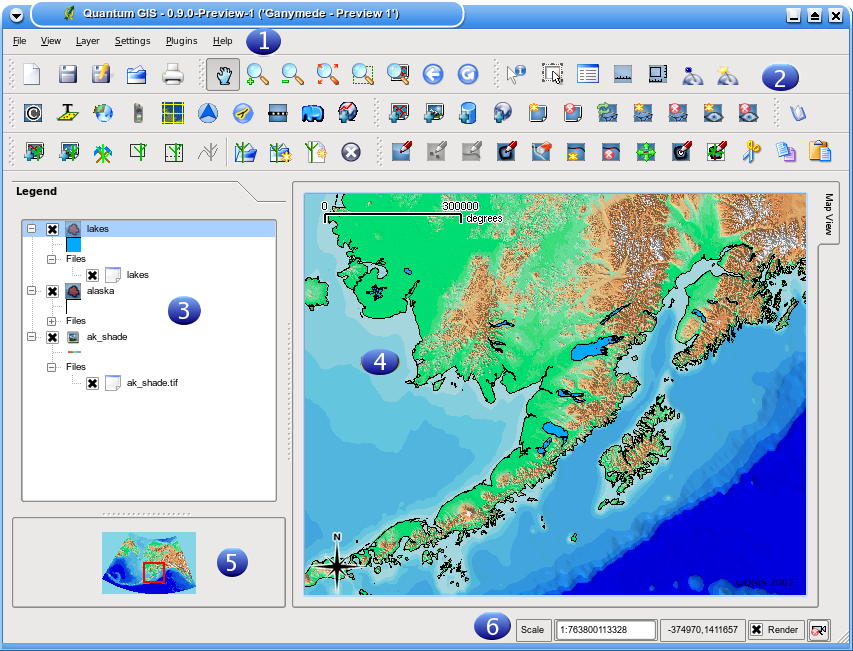
\includegraphics[clip=true, width=17cm]{startup09}
\end{center} 
\end{figure}

\textbf{Note:} Your window decorations (title bar, etc.) may appear
different depending on your operating system and window manager.

The QGIS GUI is divided into six areas:

\begin{tabbing}
1. Menu Bar \hspace{3cm}\= 4. Map View \\
2. Tool Bar \hspace{3cm}\> 5. Map Overview  \\
3. Map Legend \hspace{3cm}\> 6. Status Bar   
\end{tabbing}

These six components of the QGIS interface are described in more detail in
the following sections.

\subsubsection{Menu Bar}\label{label_menubar}
\index{menus}

The menu bar provides access to various QGIS features using a standard 
hierarchical menu. The top-level menus and a summary of some of the
functions provided are:

\begin{itemize}

\item \menuopt{File}
\begin{itemize}
\item \menuopt{New Project}          - see Section \ref{sec:projects}
\item \menuopt{Open Project}         - see Section \ref{sec:projects}
\item \menuopt{Open Recent Projects} - see Section \ref{sec:projects}
\item \menuopt{Save Project}         - see Section \ref{sec:projects}
\item \menuopt{Save Project As}      - see Section \ref{sec:projects}
\item \menuopt{Save as Image}
\item \menuopt{Export to MapServer Map}       - see Section \ref{sec:mapserver_export}
\item \menuopt{Print}                         - see Section \ref{label_mapcomposer}
\item \menuopt{Exit}
\end{itemize}

\item \textbf{View}
\begin{itemize}
\item \menuopt{Zoom Full}
\item \menuopt{Zoom To Selection}
\item \menuopt{Zoom To Layer}
\item \menuopt{Zoom Last}
\item \menuopt{Refresh}
\item \menuopt{Show Bookmarks}
\item \menuopt{New Bookmark}
\item \menuopt{Show most toolbars}
\item \menuopt{Hide most toolbars}
\item \menuopt{Toolbar Visibility} 
\end{itemize}

\item \textbf{Layer}
\begin{itemize}
\item \menuopt{Add a Vector Layer}       - see Section \ref{label_workingvector}
\item \menuopt{Add a Raster Layer}       - see Section \ref{label_raster}
\item \menuopt{Add a PostGIS Layer}      - see Section \ref{label_postgis}
\item \menuopt{Add a WMS Layer}          - see Section \ref{sec:ogc-wms}
\item \menuopt{Remove Layer}
\item \menuopt{New Vector Layer}          	- see Section \ref{sec:create shape}
\item \menuopt{In Overview}
\item \menuopt{Add All To Overview}
\item \menuopt{Remove All From Overview}
\item \menuopt{Hide All Layers}
\item \menuopt{Show All Layers}
\end{itemize}

\item \textbf{Settings}
\begin{itemize}
\item \menuopt{Project Properties}  - see Section \ref{sec:projects}
\item \menuopt{Custom Projection}   - see Section \ref{sec:customprojections}
\item \menuopt{Options}             - see Section \ref{subsec:gui_options}
\end{itemize}

\item \textbf{Plugins} - (Futher menu items are added by plugins as they are loaded.)
\begin{itemize}
\item \menuopt{Plugin Manager}          	   - see Section \ref{sec:managing_plugins}
\end{itemize}          	

\item \textbf{Help}
\begin{itemize}
\item \menuopt{Help Contents}
\item \menuopt{QGIS Homepage}
\item \menuopt{Check QGIS Version}
\item \menuopt{About}
\end{itemize}

\end{itemize}

%See Appendix \ref{app_menu} for complete descriptions of the menu items.

\subsubsection{Toolbars}\label{label_toolbars}
\index{toolbars}

The toolbars provide access to most of the same functions as the menus,
plus additional tools for interacting with the map. Each toolbar item has
popup help available. Hold your mouse over the item and a short description of
the tool's purpose will be displayed. 

Every menubar can be moved around according to your needs. Additionally every
menubar can be switched off using your right mouse button context menu holding
the mouse over the toolbars.

\begin{Tip}
\caption{\textsc{Reappearing toolbars}} \index{layout!toolbars}
\qgistip{If you have accidentally hidden all your toolbars, you can get them back by
choosing \menuopt{Show most toolbars} from the \menuopt{View} menu.}
\end{Tip}

\subsubsection{Map Legend}\label{label_legend}
\index{legend}

% TODO The new legend features need to be described here briefly.
% Marco, would you make a start what is new in the legend?!
The map legend area is used to set the visibility and z-ordering of layers.
Z-ordering means that layers listed nearer the top of the legend are drawn
over layers listed lower down in the legend. The checkbox in each legend
entry can be used to show or hide the layer.\index{layer!visibility}

Layers can be grouped in the legend window by adding a layer group and dragging layers 
into the group. To do so, go with the mouse to the legend window, right click, choose \menuopt{Add group}. 
A new folder appears. Now drag the layers to the folder symbol. It is then possible to toggle the 
visibility of all the layers in the group with one click. To bring layers out of a group, go with 
the mouse to the layer symbol, right click, choose \menuopt{Make to toplevel item}. To give the folder a 
new name, choose \menuopt{Rename} in the right click menu of the group.

The content of the right mouse button context menu depends on if the loaded legend item you hold your 
mouse over is a raster or a vector layer. For GRASS vector layers the \menuopt{toggle editing} is not 
available. See section \ref{grass_digitising} for infos on editing GRASS vector layers. 

\begin{itemize}

\item \textbf{Right mouse button menu for raster layers}
\begin{itemize}
\item \menuopt{Zoom to layer extent}
\item \menuopt{Zoom to best scale (100\%)}
\item \menuopt{Show in overview}
\item \menuopt{Remove}
\item \menuopt{Properties}
\item \menuopt{Rename}
\item \menuopt{Add Group}
\item \menuopt{Expand all}
\item \menuopt{Collapse all}
\item \menuopt{Show file groups}
\end{itemize}

\item \textbf{Right mouse button menu for vector layers}
\begin{itemize}
\item \menuopt{Zoom to layer extent}
\item \menuopt{Show in overview}
\item \menuopt{Remove}
\item \menuopt{Open attribute table}
\item \menuopt{Toggle editing (not available for GRASS layers)}
\item \menuopt{Save as shapefile}
\item \menuopt{Save selection as shapefile}
\item \menuopt{Properties}
\item \menuopt{Rename}
\item \menuopt{Add Group}
\item \menuopt{Expand all}
\item \menuopt{Collapse all}
\item \menuopt{Show file groups}
\end{itemize}

\item \textbf{Right mouse button menu for layer groups} 
\begin{itemize}
\item \menuopt{Remove}
\item \menuopt{Rename}
\item \menuopt{Add Group}
\item \menuopt{Expand all}
\item \menuopt{Collapse all}
\item \menuopt{Show file groups}
\end{itemize}

\end{itemize}

If several vector data sources have the same vector type and the same attributes, their 
symbolisations may be grouped. This means that if the symbolisation of one data source is 
changed, the others automatically have the new symbolisation as well. To group symbologies, open 
the right click menu in the legend window and choose \menuopt{Show file groups}. The file groups of the 
layers appear. It is now possible to drag a file from one file group into another one. If this is done, 
the symbologies are grouped. Note that QGIS only permits the drag if the two layers are able to share 
symbology (same vector type and same attributes).  

%% isn't included in Titan anymore, except for an "toggle overview"
%Each legend entry can show the following mini icons:
%
%
\includegraphics[width=0.7cm]{pyramid} This is a raster
%that has pyramids built for it to improve rendering efficiency (see
%Section \ref{raster_pyramids}).\\
%
\includegraphics[width=0.7cm]{no_pyramid} This is a
%raster that has no pyramid layers (see Section \ref{raster_pyramids}).\\
%
\includegraphics[width=0.7cm]{inoverview} This layer is
%shown in the overview map area as well as in the main map window.\\
%
\includegraphics[width=0.7cm]{editable} This is a vector
%layer that is currently enabled for editing.\\

\subsubsection{Map View}\label{label_mapview}
\index{map!view}

This is the 'business end' of QGIS - maps are displayed in this area! The
map displayed in this window will depend on the vector and raster layers you
have chosen to load (see sections that follow for more information on how to
load layers). The map view can be panned (shifting the focus of the map display
to another region) and zoomed in and out. Various other operations can be
performed on the map as described in the toolbar description above.  The map
view and the legend are tightly bound to each other - the maps in view reflect
changes you make in the legend area.  

\begin{Tip}\caption{\textsc{Zooming the Map with the Mouse
Wheel}}\index{zoom!mouse wheel}
\qgistip{You can use the mouse wheel to zoom in and out on the map. Place
the mouse cursor inside the map area and roll it forward (away from you) to
zoom in and backwards (towards you) to zoom out. The mouse cursor is the 
center where the zoom occurs. You can customize the behavior of the mouse
wheel zoom using the \tab{Map tools} tab under the \menuopt{Settings} ->\menuopt{Options} menu.  }
\end{Tip}

\subsubsection{Map Overview}\label{label_mapoverview}
\index{map!overview}

The map overview area provides a full extent view of layers added to it.
Within the view is a rectangle showing the current map extent. This allows
you to quickly determine which area of the map you are currently viewing. Note
that labels are not rendered to the map overview even if the layers in the
map overview have been set up for labeling. 
You can add a single layer to the
overview by right-clicking on it in the legend and choosing \menuopt{Show in overview}. You can also add or remove all layers to the overview using the
Overview tools on the toolbar.

You can also grab the red rectangle showing your current extent and pan around; the
map view will update accordingly.

\subsubsection{Status Bar}\label{label_statusbar}

The status bar shows you your current position in map coordinates (e.g.
meters or decimal degrees) as the mouse pointer is moved across the map view.
The status bar also shows the view extents of the map view as you pan and
zoom in and out. A progress bar in the status bar shows progress of rendering
as each layer is drawn to the map view. In some cases, such as the gathering
of statistics in raster layers, the progress bar will be used to show the
status of lengthy operations. On the right side of the status bar is a small
checkbox which can be used to temporarily prevent layers being rendered to the
map view (see Section \ref{subsec:redraw_events} below). At the far right of
the status bar is a projector icon. Clicking on this opens the projection
properties for the current project.

\subsection{Rendering}\label{subsec:redraw_events}\index{rendering}

By default, QGIS renders all visible layers whenever the map canvas must be
refreshed. The events that trigger a refresh of the map canvas include:

\begin{itemize}
\item Adding a layer
\item Panning or zooming
\item Resizing the QGIS window
\item Changing the visibility of a layer or layers
\end{itemize}

QGIS allows you to control the rendering process in a number of ways.

\subsubsection{Scale Dependent Rendering}\index{rendering!scale dependent}
\label{label_scaledepend}

Scale dependent rendering allows you to specify the minimum and maximum
scales at which a layer will be visible.  To set scale dependency rendering,
open the properties dialog by double-clicking on the layer in the legend. On
the \tab{General} tab, set the minimum and maximum scale values and then
click on the \checkbox{Use scale dependent rendering} checkbox.

You can determine the scale values by first zooming to the level you want
to use and noting the scale value in the QGIS status bar.\index{scale}

\subsubsection{Controlling Map Rendering}\label{label_controlmap}

Map rendering can be controlled in the following ways:

\minisec{Suspending Rendering}\index{rendering!suspending}
\label{label_suspendrender}

To suspend rendering, click the \checkbox{Render} checkbox in the lower right
corner of the statusbar. When the \checkbox{Render} box is not checked, QGIS
does not redraw the canvas in response to any of the events described in
Section \ref{subsec:redraw_events}. Examples of when you might want to suspend
rendering include:

\begin{itemize}
\item Add many layers and symbolize them prior to drawing
\item Add one or more large layers and set scale dependency before drawing
\item Add one or more large layers and zoom to a specific view before
drawing
\item Any combination of the above
\end{itemize}

Checking the \checkbox{Render} box enables rendering and causes and immediate
refresh of the map canvas.

\minisec{Setting Layer Add Option}\label{label_settinglayer}
\index{rendering!options}\index{layers!initial visibility}

You can set an option to always load new layers without drawing them. This
means the layer will be added to the map, but its visibility checkbox in the
legend will be unchecked by default. To set this option, choose
\menuopt{Options} from the \menuopt{Settings} menu and click on the
\tab{Rendering} tab. Uncheck the \checkbox{By default new layers added to the map 
should be
displayed} checkbox. Any layer added to the map will be off (invisible) by
default.

%\minisec{Stopping Rendering}\index{rendering!halting}
%\label{label_stoprender}
%
%To stop the map drawing, press the ESC key. This will halt the refresh of
%the map canvas and leave the map partially drawn. It may take a bit of time
%between pressing ESC and the time the map drawing is halted.
%
%\textbf{NOTE}: It is currently not possible to stop rendering - this was disabled 
%in qt4 port because of User Interface (UI) problems and crashes.

\minisec{Updating the Map Display During Rendering}
\label{label_updatemap}\index{rendering!update during drawing}

You can set an option to update the map display as features are drawn. By
default, QGIS does not display any features for a layer until the entire
layer has been rendered. To update the display as features are read from the
datastore, choose \menuopt{Options} from the \menuopt{Settings} menu and
click on the \tab{Rendering} tab. Set the feature count to an
appropriate value to update the display during rendering. Setting a value of 0
disables update during drawing (this is the default). Setting a value too low
will result in poor performance as the map canvas is continually updated
during the reading of the features. A suggested value to start with is 500. 

\subsection{Measuring}\label{sec:measure}\index{measure}

Measuring works within projected coordinate systems only (e.g., UTM). If 
the loaded map is defined with a geographic coordinate system
(latitude/longitude), the results from line or area measurements will be 
incorrect. To fix this you need to set an appropriate map coordinate system.

\subsubsection{Measure length}\index{measure:line length}

\includegraphics[width=0.7cm]{measureline} QGIS is also able to measure real distances between given 
points according to a defined ellipsoid. Therefore choose \menuopt{Options} from the \menuopt{Settings} menu, 
click on the \tab{Map tools} tab and choose the appropriate ellipsoid. The tool then allows you to 
click points on the map. Each segment-length shows up in the measure-window and additionaly the total 
length is printed. To stop measuring click your right mouse button. 

\subsubsection{Measure areas}\index{measure:areas}

\includegraphics[width=0.7cm]{measurearea} Also areas can be measured. The window only shows the
accumulated area-size in the measure window (see figure \ref{fig:measure}).

% measure-tools side by side
\begin{figure}[h]
\caption{Measure tools in action} \label{fig:measure}
\centering
   \subfigure[Measure lines] {\label{subfig:measure_line}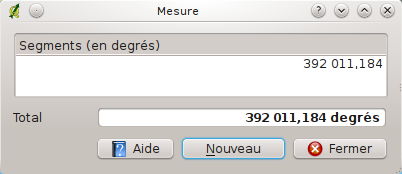
\includegraphics[clip=true, width=0.4\textwidth]{measure_line}}\goodgap
   \subfigure[Measure areas]{\label{subfig:measure_area}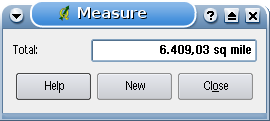
\includegraphics[clip=true, width=0.4\textwidth]{measure_area}}
\end{figure}

\subsection{Projects}\label{sec:projects}\index{projects}

The state of your QGIS session is considered a Project.  QGIS
works on one project at a time.  Settings are either considered
as being per-project, or as a default for new projects (see
Section \ref{subsec:gui_options}).

QGIS can save the state of your workspace into a project file using
the menu option \menuopt{File} -> \menuopt{Save Project}.

Loading saved projects is a similar process.

The kinds of information saved in a project file include:

\begin{itemize}
\item Layers added
\item Layer properties, including symbolization
\item Projection for the map view
\item Last viewed extent
\end{itemize}

The project file is saved in XML format, so it is possible to edit
the file outside QGIS if you know what you are doing.  

The file format was updated several times compared to earlier QGIS versions. Project files 
from older QGIS versions may not work properly anymore.

\subsection{GUI Options}
\label{subsec:gui_options}

\includegraphics[width=0.7cm,clip=true]{options} Some basic options for QGIS
can be selected using the Options dialog. Select the \menuopt{Settings} entry
from the menu and choose \menuopt{Options} or press \keystroke{Alt-O}. The tabs where you can 
optmize your options are:

\minisec{General Tab}

\begin{itemize}
\item Ask to save project changes when required
\end{itemize}

\minisec{Appearance Tab}

\begin{itemize}
\item Hide or show splash screen at startup
\item Change the icon theme 
\item Change Selection and backgroud Color
\item Make layer names appear with Capitals
\end{itemize}

\minisec{Rendering Tab}

\begin{itemize}
\item Update features during drawing or not until all features have been read.
\item Set new layer visible or unvisible when loaded 
\item Make lines appear less jagged at the expense of some drawing performance
\item Fix problems with incorrectly filled polygons
\item Continously redraw when dragging the legend/map divider 
\end{itemize}

\minisec{Map tools Tab}

\begin{itemize}
\item Define Search Radius as a percentage of the map width
\item Define Ellipsoid for distance calculations
\item Set Rubberband Color for Measure Tool
\item Define Mouse wheel action (Zoom, Zoom and recenter, Nothing)
\item Set Zoom factor for wheel mouse
\end{itemize}

\minisec{Projection Tab}

\begin{itemize}
\item Define what to do, when a layer is loaded without projection information
\begin{itemize}
\item Prompt for projection
\item Project wide default projection will be used
\item Global default projection displayed below will be used
\end{itemize}
\end{itemize}

\minisec{Locale Tab}

\begin{itemize}
\item Overwrite system locale and use defined locale instead
\item Information about active system locale
\end{itemize}

\minisec{Help Browser Tab}

\begin{itemize}
\item Define Browser to display help documents
\end{itemize}


You can modify the options according to your needs. Some of the changes may 
require a restart of QGIS before they will be effective.

On GNU/Linux everything is saved in:
\begin{verbatim}
$HOME/.config/QuantumGIS/qgis.conf
\end{verbatim}
This is a normal text file consisting of blocks, where QGIS saves its current
display options, PostGIS and WMS connections, and other settings.

On Windows settings are stored in the registry under:
\begin{verbatim}
\\HKEY_CURRENT_USER\Software\QuantumGIS\qgis
\end{verbatim}

On OS X you can find your settings in:
\begin{verbatim}
$HOME/Library/Preferences/org.qgis.qgis.plist
\end{verbatim}


\subsection{Spatial Bookmarks}\label{sec:bookmarks}
\index{bookmarks}
\index{spatial bookmarks|\see{bookmarks}}

Spatial Bookmarks allow you to ``bookmark'' a geographic location and return to it later.

\subsubsection{Creating a Bookmark}
To create a bookmark:
\begin{enumerate}
\item Zoom or pan to the area of interest.
\item Select the menu option \menuopt{View} -> \menuopt{New Bookmark} or press \keystroke{Ctrl-B}.
\item Enter a descriptive name for the bookmark (up to 255 characters).
\item Click \button{OK} to add the bookmark or \button{Cancel} to exit without adding the bookmark.
\end{enumerate}

Note that you can have multiple bookmarks with the same name.

\subsubsection{Working with Bookmarks}
To use or manage bookmarks, select the menu option \menuopt{View} -> \menuopt{Show Bookmarks}.
The bookmarks dialog allows you to zoom to or delete a bookmark.
You can not edit the bookmark name or coordinates.

\subsubsection{Zooming to a Bookmark}
From the Bookmarks dialog, select the desired bookmark by clicking on it, 
then click the \button{Zoom To} button.
You can also zoom to a bookmark by double-clicking on it.

\subsubsection{Deleting a Bookmark}
To delete a bookmark from the Bookmarks dialog, click on it then click the \button{Delete} button.
Confirm your choice by clicking \button{Yes} or cancel the delete by clicking \button{No}.

%  !TeX  root  =  user_guide.tex 

\chapter{Features at a Glance}\label{feature_glance}

% when the revision of a section has been finalized, 
% comment out the following line:
%\updatedisclaimer

After a first and simple sample session in Section \ref{label_getstarted} we now 
want to give you a more detailed overview of the features of QGIS. 
Most features presented in the following chapters will be explained and described in 
own sections later in the manual.

\section{Starting and Stopping QGIS}\label{label_startinqgis}

In Section \ref{samplesession} you already learned how to start QGIS. We will 
repeat this here and you will see that QGIS also provides further command line options. 

\begin{itemize}
\item \nix{Assuming that QGIS is installed in the PATH, you can start QGIS 
by typing: \usertext{qgis}  at a command prompt or by double clicking on the QGIS
application link (or shortcut) on the desktop or in the application menu.} 
\item \win{Start QGIS using the Start menu or desktop shortcut, 
or double click on a QGIS project file.}
\item \osx{Double click the icon in your Applications folder. If you need to start QGIS 
in a shell, run /path-to-installation-executable/Contents/MacOS/Qgis.}
\end{itemize} 

To stop QGIS, click the menu options \{\nix{}\win{File} \osx{QGIS}\} > Quit,
or use the shortcut \keystroke{Ctrl+Q}.

\subsection{Command Line Options}\index{command line options}
\label{label_commandline}

\nix QGIS supports a number of options when started from the command line. To
get a list of the options, enter \usertext{qgis ---help} on the command line.
The usage statement for QGIS is:

\small
\begin{verbatim}
qgis --help
Quantum GIS - 1.5.0-Tethys 'Tethys' (exported)
Quantum GIS (QGIS) is a viewer for spatial data sets, including
raster and vector data.
Usage: qgis [options] [FILES]
  options:
        [--snapshot filename]           emit snapshot of loaded datasets to given file
        [--width width]                 width of snapshot to emit
        [--height height]               height of snapshot to emit
        [--lang language]               use language for interface text
        [--project projectfile]         load the given QGIS project
        [--extent xmin,ymin,xmax,ymax]  set initial map extent
        [--nologo]                      hide splash screen
        [--help]                        this text

  FILES:
    Files specified on the command line can include rasters,
    vectors, and QGIS project files (.qgs):
     1. Rasters - Supported formats include GeoTiff, DEM
        and others supported by GDAL
     2. Vectors - Supported formats include ESRI Shapefiles
        and others supported by OGR and PostgreSQL layers using
        the PostGIS extension
\end{verbatim}
\normalsize

\begin{Tip} \caption{\textsc{Example Using command line arguments}}
You can start QGIS by specifying one or more data files
on the command line. For example, assuming you are in the 
qgis\_sample\_data directory, you could start QGIS with a vector layer 
and a raster file set to load on startup using the following command: 
\usertext{qgis ./raster/landcover.img ./gml/lakes.gml}
\end{Tip}

\minisec{Command line option \usertext{---snapshot}}
This option allows you to create a snapshot in PNG format from the current view.
This comes in handy when you have a lot of projects and want to 
generate snapshots from your data.

Currently it generates a PNG-file with 800x600 pixels. This can be adapted
using the \usertext{---width} and \usertext{---height} command line
arguments. A filename can be added after \usertext{---snapshot}.

\minisec{Command line option \usertext{---lang}}
Based on your locale QGIS, selects the correct localization. If you would like 
to change your language, you can specify a language code. For example: 
\usertext{---lang=it}
starts QGIS in italian localization. A list of currently supported
languages with language code and status is provided at
\url{http://www.qgis.org/wiki/GUI_Translation_Progress} 

\minisec{Command line option \usertext{---project}}
Starting QGIS with an existing project file is also possible. Just
add the command line option \usertext{---project} followed by your project
name and QGIS will open with all layers loaded described in the given file.

\minisec{Command line option \usertext{---extent}}
To start with a specific map extent use this option. You need to add the bounding box of your extent in the following order separated by a comma:
\begin{verbatim}
--extent xmin,ymin,xmax,ymax
\end{verbatim}

\minisec{Command line option \usertext{---nologo}}
This command line argument hides the splash screen when you start QGIS.

\section{QGIS GUI}\index{main window}
\label{label_qgismainwindow}

When QGIS starts, you are presented with the GUI as shown below
(the numbers 1 through 6 in yellow ovals refer to the six major areas of the
interface as discussed below):

\begin{figure}[ht]
   \centering
    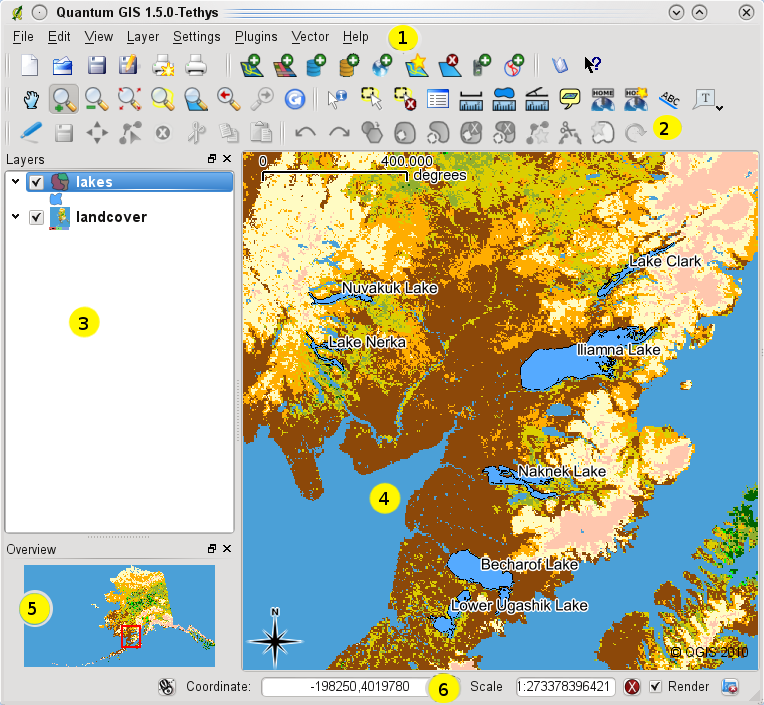
\includegraphics[clip=true, width=12cm]{startup}
    \caption{QGIS GUI with Alaska sample data \nixcaption (KDE)} \label{fig:startup} 
\end{figure}

\textbf{Note:} Your window decorations (title bar, etc.) may appear
different depending on your operating system and window manager.\\

The QGIS GUI is divided into six areas:

\begin{tabular}{p{5cm} p{5cm}}
%\centering
1. Menu Bar & 4. Map View \\
2. Tool Bar & 5. Map Overview \\
3. Map Legend & 6. Status Bar \\ 
\end{tabular}

These six components of the QGIS interface are described in more detail in
the following sections. Two more sections present keyboard shortcuts and 
context help.

% \newpage

\subsection{Menu Bar}\label{label_menubar}
\index{menus}

The menu bar provides access to various QGIS features using a standard 
hierarchical menu. The top-level menus and a summary of some of the
menu options are listed below, together with the icons of the corresponding
tools as they appear on the toolbar, as well as keyboard
shortcuts.\footnote{Keyboard shortcuts can now be configured manually
(shortcuts presented in this section are the defaults), using the Configure 
Shortcuts tool under Settings Menu.}
Although most menu options have a corresponding tool and vice-versa,
the menus are not organized quite like the toolbars. 
The toolbar containing the tool is listed after each menu option as a checkbox
entry. For more information about tools and toolbars, see Section
\ref{label_toolbars}.

\begin{tabbing}
\hspace{5.5cm}\=\hspace{3cm}\=\hspace{3.5cm}\= \kill
\hspace{1cm} Menu Option \> Shortcut \> Reference \> Toolbar\\
\end{tabbing}

\begin{itemize}
\item \mainmenuopt{File}
\begin{tabbing}
\hspace{4.5cm}\=\hspace{3cm}\=\hspace{3.5cm}\= \kill
\dropmenuopttwo{mActionFileNew}{New Project}
	\> \keystroke{Ctrl+N}
	\> see Section \ref{sec:projects}
	\> \dropmenucheck{File} \\
\dropmenuopttwo{mActionFileOpen}{Open Project}
	\> \keystroke{Ctrl+O}
	\> see Section \ref{sec:projects}
	\> \dropmenucheck{File} \\
\dropmenuopt{Open Recent Projects}
	\>
	\> see Section \ref{sec:projects} \\
\dropmenuopttwo{mActionFileSave}{Save Project}
	\> \keystroke{Ctrl+S}
	\> see Section \ref{sec:projects}
	\> \dropmenucheck{File} \\
\dropmenuopttwo{mActionFileSaveAs}{Save Project As}
	\> \keystroke{Ctrl+Shift+S}
  \> see Section \ref{sec:projects}
	\> \dropmenucheck{File} \\
\dropmenuopttwo{mActionSaveMapAsImage}{Save as Image}
	\>
	\> see Section \ref{sec:output} \\
\dropmenuopttwo{mActionNewComposer}{New Print Composer}
        \> \keystroke{Ctrl+P}
        \> see Section \ref{label_printcomposer}
        \> \dropmenucheck{File} \\
\dropmenuopttwo{mActionComposerManager}{Composer manager}
	\> 
	\> see Section \ref{label_printcomposer}
	\> \dropmenucheck{File} \\
\dropmenuopt{Print Composers}
	\>
	\> see Section \ref{label_printcomposer} \\
\dropmenuopttwo{mActionFileExit}{Exit} 
	\> \keystroke{Ctrl+Q} \\
\end{tabbing}

\item \mainmenuopt{Edit}
\begin{tabbing}
\hspace{4.5cm}\=\hspace{3cm}\=\hspace{3.5cm}\= \kill
\dropmenuopttwo{mActionUndo}{Undo}
        \> \keystroke{Ctrl+Z}
        \> see Section \ref{sec:advanced_edit}
        \> \dropmenucheck{Advanced Digitizing} \\
\dropmenuopttwo{mActionRedo}{Redo}
        \> \keystroke{Ctrl+Shift+Z}
        \> see Section \ref{sec:advanced_edit}
        \> \dropmenucheck{Advanced Digitizing} \\
\dropmenuopttwo{mActionEditCut}{Cut Features} 
	\> \keystroke{Ctrl+X}
	\> see Section \ref{sec:edit_existing_layer} 
	\> \dropmenucheck{Digitizing} \\
\dropmenuopttwo{mActionEditCopy}{Copy Features}
	\> \keystroke{Ctrl+C}
	\> see Section \ref{sec:edit_existing_layer} 
	\> \dropmenucheck{Digitizing} \\
\dropmenuopttwo{mActionEditPaste}{Paste Features} 
	\> \keystroke{Ctrl+V}
	\> see Section \ref{sec:edit_existing_layer} 
	\> \dropmenucheck{Digitizing} \\
\dropmenuopttwo{mActionEditPaste}{Move Feature}
        \> 
        \> see Section \ref{sec:edit_existing_layer}
        \> \dropmenucheck{Digitizing} \\
\dropmenuopttwo{mActionDeleteSelected}{Delete Selected}
        \> 
        \> see Section \ref{sec:edit_existing_layer}
        \> \dropmenucheck{Digitizing} \\
\dropmenuopttwo{mActionSimplify}{Simplify Feature}
        \>
        \> see Section \ref{sec:advanced_edit}
        \> \dropmenucheck{Advanced Digitizing} \\
\dropmenuopttwo{mActionAddRing}{Add Ring}
        \>
        \> see Section \ref{sec:advanced_edit}
        \> \dropmenucheck{Advanced Digitizing} \\
\dropmenuopttwo{mActionAddIsland}{Add Part}
        \>
        \> see Section \ref{sec:advanced_edit}
        \> \dropmenucheck{Advanced Digitizing} \\
\dropmenuopttwo{mActionDeleteRing}{Delete Ring}
        \>
        \> see Section \ref{sec:advanced_edit}
        \> \dropmenucheck{Advanced Digitizing} \\
\dropmenuopttwo{mActionDeletePart}{Delete Part}
        \>
        \> see Section \ref{sec:advanced_edit}
        \> \dropmenucheck{Advanced Digitizing} \\
\dropmenuopttwo{mActionReshape}{Reshape Features}
        \>
        \> see Section \ref{sec:advanced_edit}
        \> \dropmenucheck{Advanced Digitizing} \\
\dropmenuopttwo{mActionSplitFeatures}{Split Features}
        \>
        \> see Section \ref{sec:advanced_edit}
        \> \dropmenucheck{Advanced Digitizing} \\
\dropmenuopttwo{mActionMergeFeatures}{Merge selected Features}
        \>
        \> see Section \ref{sec:advanced_edit}
        \> \dropmenucheck{Advanced Digitizing} \\
\dropmenuopttwo{mActionNodeTool}{Node Tool}
        \>
        \> see Section \ref{sec:edit_existing_layer}
        \> \dropmenucheck{Digitizing} \\
\dropmenuopttwo{mActionRotatePointSymbols}{Rotate Point Symbols}
        \>
        \> see Section \ref{sec:advanced_edit}
        \> \dropmenucheck{Advanced Digitizing} \\
\end{tabbing}

After activating \toolbtntwo{mActionToggleEditing}{toogle editing} mode
for a layer, you will find a capture feature icon in the \mainmenuopt{Edit}
menu depending on the layer type (point, line or polygon). \\

\begin{tabbing}
\hspace{4.5cm}\=\hspace{3cm}\=\hspace{3.5cm}\= \kill
\dropmenuopttwo{mActionCapturePoint}{Capture Point}
        \>
        \> see Section \ref{sec:edit_existing_layer}
        \> \dropmenucheck{Digitizing} \\
\dropmenuopttwo{mActionCaptureLine}{Capture Line}
        \>
        \> see Section \ref{sec:edit_existing_layer}
        \> \dropmenucheck{Digitizing} \\
\dropmenuopttwo{mActionCapturePolygon}{Capture Polygon}
        \>
        \> see Section \ref{sec:edit_existing_layer}
        \> \dropmenucheck{Digitizing} \\
\end{tabbing}


\item \mainmenuopt{View}
\begin{tabbing}
\hspace{4.5cm}\=\hspace{3cm}\=\hspace{3.5cm}\= \kill
\dropmenuopttwo{mActionPan}{Pan Map}
	\>
	\> \> \dropmenucheck{Map Navigation} \\
\dropmenuopttwo{mActionZoomIn}{Zoom In}
	\> \keystroke{Ctrl++}
	\> \> \dropmenucheck{Map Navigation} \\
\dropmenuopttwo{mActionZoomOut}{Zoom Out}
	\> \keystroke{Ctrl+-}
	\> \> \dropmenucheck{Map Navigation} \\
\dropmenuopttwo{mActionSelect}{Select Features}
	\>
	\> \> \dropmenucheck{Attributes} \\
\dropmenuopttwo{mActionDeselectAll}{Deselect Features}
        \>
        \> \> \dropmenucheck{Attributes} \\
\dropmenuopttwo{mActionIdentify}{Identify Features}
	\> \keystroke{I}
	\> \> \dropmenucheck{Attributes} \\
\dropmenuopttwo{mActionMeasure}{Measure Line}
	\> \keystroke{M}
	\> \> \dropmenucheck{Attributes} \\
\dropmenuopttwo{mActionMeasureArea}{Measure Area}
	\> \keystroke{J}
	\> \> \dropmenucheck{Attributes} \\
\dropmenuopttwo{mActionOpenTable}{Zoom Full}
	\> \keystroke{F}
	\> \> \dropmenucheck{Map Navigation} \\
\dropmenuopttwo{mActionZoomToLayer}{Zoom To Layer}
	\>
	\> \> \dropmenucheck{Map Navigation} \\
\dropmenuopttwo{mActionZoomToSelected}{Zoom To Selection}
	\> \keystroke{Ctrl+J}
	\> \> \dropmenucheck{Map Navigation} \\
\dropmenuopttwo{mActionZoomLast}{Zoom Last}
	\>
	\> \> \dropmenucheck{Map Navigation} \\
\dropmenuopttwo{mActionZoomNext}{Zoom Next}
	\>
	\> \> \dropmenucheck{Map Navigation} \\
\dropmenuopt{Zoom Actual Size}
	\>
	\> \>  \\
\dropmenuopttwo{mActionMapTips}{Map Tips}
	\>
	\> \> \dropmenucheck{Attributes} \\
\dropmenuopttwo{mActionNewBookmark}{New Bookmark}
	\> \keystroke{Ctrl+B}
	\> see Section \ref{sec:bookmarks} 
\> \dropmenucheck{Attributes} \\
\dropmenuopttwo{mActionShowBookmarks}{Show Bookmarks}
	\> \keystroke{B}
	\> see Section \ref{sec:bookmarks} 
	\> \dropmenucheck{Attributes} \\
\dropmenuopttwo{mActionDraw}{Refresh}
	\> \keystroke{Ctrl+R}
	\> \> \dropmenucheck{Map Navigation} \\
\end{tabbing}

\item \mainmenuopt{Layer}
\begin{tabbing}
\hspace{5cm}\=\hspace{3cm}\=\hspace{3.5cm}\= \kill
\dropmenuopttwo{mActionNewVectorLayer}{New Vector Layer}
	\> \keystroke{Ctrl+Shift+N}
	\>          	
	see Section \ref{sec:create shape}
	\> \dropmenucheck{Manage Layers} \\
\dropmenuopttwo{mActionAddNonDbLayer}{Add Vector Layer}       
	\> \keystroke{Ctrl+Shift+V}
	\>          	
	see Section \ref{label_workingvector}
	\> \dropmenucheck{File} \\
\dropmenuopttwo{mActionAddRasterLayer}{Add Raster Layer}       
	\> \keystroke{Ctrl+Shift+R}
	\>          	
	see Section \ref{label_raster}
	\> \dropmenucheck{File} \\
\dropmenuopttwo{mActionAddLayer}{Add PostGIS Layer}      
	\> \keystroke{Ctrl+Shift+D}
	\>          	
	see Section \ref{label_postgis}
        \> \dropmenucheck{File} \\
\dropmenuopttwo{mActionAddSpatiaLiteLayer}{Add SpatiaLite Layer}
        \> \keystroke{Ctrl+Shift+L}
        \>
        see Section \ref{label_spatialite}
	\> \dropmenucheck{File} \\
\dropmenuopttwo{mActionAddWmsLayer}{Add WMS Layer}          
	\> \keystroke{Ctrl+Shift+W}
	\>          	
	see Section \ref{sec:ogc-wms}
	\> \dropmenucheck{File} \\
\dropmenuopttwo{mActionOpenTable}{Open Attribute Table}
	\> \>
	\> \dropmenucheck{Attributes} \\
\dropmenuopttwo{mActionToggleEditing}{Toggle editing}
	\> \>
	\> \dropmenucheck{Digitizing} \\
\dropmenuopt{Save As Shapefile}
	\\
\dropmenuopt{Save Selection As Shapefile}
	\\
\dropmenuopttwo{mActionRemoveLayer}{Remove Layer}
	\> \keystroke{Ctrl+D}
	\>          	
	\> \dropmenucheck{Properties} \\
\dropmenuopt{Properties}
	\\
\dropmenuopttwo{mActionInOverview}{Add to Overview}
	\> \keystroke{Ctrl+Shift+O}
	\>          	
	\> \dropmenucheck{Manage Layers} \\
\dropmenuopttwo{mActionAddAllToOverview}{Add All To Overview}
	\> 
	\>          	
	\\
\dropmenuopttwo{mActionRemoveAllFromOverview}{Remove All From Overview}
	\> 
	\>          	
	\\
\dropmenuopttwo{mActionHideAllLayers}{Hide All Layers}
	\> \keystroke{Ctrl+Shift+H}
	\>          	
	\> \dropmenucheck{Manage Layers} \\
\dropmenuopttwo{mActionShowAllLayers}{Show All Layers}
	\> \keystroke{Ctrl+Shift+S}
	\>          	
	\> \dropmenucheck{Manage Layers} \\
\end{tabbing}

\item \mainmenuopt{Settings}
\begin{tabbing}
\hspace{5cm}\=\hspace{3cm}\=\hspace{3.5cm}\= \kill
\dropmenuopt{Panels}  
	\>           
	\>          	
	\\
\dropmenuopt{Toolbars}  
	\>           
	\>          	
	\\
\dropmenuopt{Toggle Fullscreen Mode}  
	\>
	\>          	
	\\
\dropmenuopttwo{mActionProjectProperties}{Project Properties}  
	\> \keystroke{P}
	\> see Section \ref{sec:projects}
	\\
\dropmenuopttwo{mActionCustomProjection}{Custom CRS}   
	\> \> see Section \ref{sec:customprojections}
	\\
\dropmenuopt{Style Manager}
        \>
        \>
        \\
\dropmenuopttwo{mActionOptions}{Configure shortcuts}
        \>
        \>
        \\
\dropmenuopttwo{mActionOptions}{Options}             
	\> \> see Section \ref{subsec:gui_options}
	\\
\end{tabbing}

\item \mainmenuopt{Plugins} - (Futher menu items are added by plugins as they are loaded.)
\begin{tabbing}
\hspace{5cm}\=\hspace{3cm}\=\hspace{3.5cm}\= \kill
\dropmenuopttwo{mActionShowPluginManager}{Manage Plugins}          	   
	\> \> see Section \ref{sec:managing_plugins} \dropmenucheck{Plugins}
	\\
	\dropmenuopt{Python Console}
        \> \>
        \\
\end{tabbing}          	

\item \mainmenuopt{Help}
\begin{tabbing}
\hspace{5cm}\=\hspace{3cm}\=\hspace{3.5cm}\= \kill
\dropmenuopttwo{mActionHelpContents}{Help Contents}
	\> \keystroke{F1}
	\>           	
	\> \dropmenucheck{Help}\\
\dropmenuopttwo{mActionQgisHomePage}{QGIS Home Page}
	\> \keystroke{Ctrl+H}
	\>          	
	\\
\dropmenuopttwo{mActionCheckQgisVersion}{Check QGIS Version}
	\\
\dropmenuopttwo{mActionHelpAbout}{About}
	\\
\end{tabbing}

\end{itemize}

\textbf{Note:} \nix The Menu Bar items listed above are the default ones in KDE window
manager. In GNOME, Settings menu is missing and its items are to be found
there:
\begin{tabbing}
\dropmenuopttwo{mActionProjectProperties}{Project Properties} \hspace{3cm}\=
\dropmenucheck{File menu} \\
\dropmenuopttwo{mActionOptions}{Options} \hspace{3cm}\>
\dropmenucheck{Edit}\\
\dropmenuopttwo{mActionCustomProjection}{Custom CRS}\hspace{3cm}\>
\dropmenucheck{Edit} \\
\dropmenuopt{Panels} \hspace{3cm}\>
\dropmenucheck{View} \\
\dropmenuopt{Toolbars}   \hspace{3cm}\>
\dropmenucheck{View} \\
\dropmenuopt{Toggle Fullscreen Mode} \hspace{3cm}\>
\dropmenucheck{View}
\end{tabbing}

%See Appendix \ref{app_menu} for complete descriptions of the menu items.

\subsection{Toolbars}\label{label_toolbars}
\index{toolbars}

The toolbars provide access to most of the same functions as the menus,
plus additional tools for interacting with the map. Each toolbar item has
popup help available. Hold your mouse over the item and a short description of
the tool's purpose will be displayed. 

Every menubar can be moved around according to your needs. Additionally every
menubar can be switched off using your right mouse button context menu holding
the mouse over the toolbars.

\begin{Tip}
\caption{\textsc{Restoring toolbars}} \index{layout!toolbars}
If you have accidentally hidden all your toolbars, you can get them
back by choosing menu option \mainmenuopt{Settings} > \dropmenuopt{Toolbars}.
\end{Tip}

\subsection{Map Legend}\label{label_legend}
\index{legend}

The map legend area is used to set the visibility and z-ordering of layers.
Z-ordering means that layers listed nearer the top of the legend are drawn
over layers listed lower down in the legend. The checkbox in each legend
entry can be used to show or hide the layer.\index{layer!visibility}

Layers can be grouped in the legend window by adding a layer group and dragging layers 
into the group. To do so, move the mouse pointer to the legend window, right click, choose \dropmenuopt{Add group}. 
A new folder appears. Now drag the layers onto to the folder symbol. It is then possible to toggle the 
visibility of all the layers in the group with one click. To bring layers out of a group, move 
the mouse pointer to the layer symbol, right click, and choose \dropmenuopt{Make to toplevel item}. To give the folder a 
new name, choose \dropmenuopt{Rename} in the right click menu of the group.

The content of the right mouse button context menu depends on whether the loaded legend item you hold your 
mouse over is a raster or a vector layer. For GRASS vector layers the \dropmenuopt{toggle editing} is not 
available. See section \ref{grass_digitising} for information on editing GRASS vector layers. 

\begin{itemize}

\item \textbf{Right mouse button menu for raster layers}
\begin{itemize}
\item \dropmenuopt{Zoom to layer extent}
\item \dropmenuopt{Zoom to best scale (100\%)}
\item \dropmenuopt{Show in overview}
\item \dropmenuopt{Remove}
\item \dropmenuopt{Properties}
\item \dropmenuopt{Rename}
\item \dropmenuopt{Add Group}
\item \dropmenuopt{Expand all}
\item \dropmenuopt{Collapse all}
%%\item \dropmenuopt{Show file groups}
\end{itemize}

\item \textbf{Right mouse button menu for vector layers}
\begin{itemize}
\item \dropmenuopt{Zoom to layer extent}
\item \dropmenuopt{Show in overview}
\item \dropmenuopt{Remove}
\item \dropmenuopt{Open attribute table}
\item \dropmenuopt{Toggle editing (not available for GRASS layers)}
\item \dropmenuopt{Save as shapefile}
\item \dropmenuopt{Save selection as shapefile}
\item \dropmenuopt{Properties}
%% \item \dropmenuopt{Make to toplevel item}
\item \dropmenuopt{Rename}
\item \dropmenuopt{Add Group}
\item \dropmenuopt{Expand all}
\item \dropmenuopt{Collapse all}
%%\item \dropmenuopt{Show file groups}
\end{itemize}

\item \textbf{Right mouse button menu for layer groups} 
\begin{itemize}
\item \dropmenuopt{Remove}
\item \dropmenuopt{Rename}
\item \dropmenuopt{Add Group}
\item \dropmenuopt{Expand all}
\item \dropmenuopt{Collapse all}
%%\item \dropmenuopt{Show file groups}
\end{itemize}

\end{itemize}

If several vector data sources have the same vector type and the same
attributes, their symbolisations may be grouped. This means that if the
symbolisation of one data source is changed, the others automatically have
the new symbolisation as well. To group symbologies, open the right click
menu in the legend window and choose \dropmenuopt{Add Group}. The file
groups of the layers appear. It is now possible to drag a file from one file
group into another one. If this is done, the symbologies are grouped. Note
that QGIS only permits the drag if the two layers are able to share 
symbology (same vector geometry type and same attributes).  

%% isn't included in Titan anymore, except for an "toggle overview"
%Each legend entry can show the following mini icons:
%
%
\includegraphics[width=0.7cm]{pyramid} This is a raster
%that has pyramids built for it to improve rendering efficiency (see
%Section \ref{raster_pyramids}).\\
%
\includegraphics[width=0.7cm]{no_pyramid} This is a
%raster that has no pyramid layers (see Section \ref{raster_pyramids}).\\
%
\includegraphics[width=0.7cm]{inoverview} This layer is
%shown in the overview map area as well as in the main map window.\\
%
\includegraphics[width=0.7cm]{editable} This is a vector
%layer that is currently enabled for editing.\\

\subsection{Map View}\label{label_mapview}
\index{map!view}

This is the 'business end' of QGIS - maps are displayed in this area! The
map displayed in this window will depend on the vector and raster layers you
have chosen to load (see sections that follow for more information on how to
load layers). The map view can be panned (shifting the focus of the map display
to another region) and zoomed in and out. Various other operations can be
performed on the map as described in the toolbar description above.  The map
view and the legend are tightly bound to each other - the maps in view reflect
changes you make in the legend area.  

\begin{Tip}\caption{\textsc{Zooming the Map with the Mouse
Wheel}}\index{zoom!mouse wheel}
You can use the mouse wheel to zoom in and out on the map. Place
the mouse cursor inside the map area and roll the wheel forward (away from you) to
zoom in and backwards (towards you) to zoom out. The mouse cursor position is the 
center where the zoom occurs. You can customize the behavior of the mouse
wheel zoom using the \tab{Map tools} tab under the \mainmenuopt{Settings} >
\dropmenuopt{Options} menu.
\end{Tip}

\begin{Tip}\caption{\textsc{Panning the Map with the Arrow Keys and Space
Bar}}\index{pan!arrow keys}
You can use the arrow keys to pan in the map. Place the mouse cursor 
inside the map area and click on the right arrow key to pan East, left arrow 
key to pan West, up arrow key to pan North and down arrow key to pan South. 
You can also pan the map using the space bar: just move the mouse while
holding down space bar.
\end{Tip}

\subsection{Map Overview}\label{label_mapoverview}
\index{map!overview}

The map overview panel provides a full extent view of layers added to it. It
can be selected under the menu \mainmenuopt{Settings} >\dropmenuopt{Panels}.
Within the view is a rectangle showing the current map extent. This allows
you to quickly determine which area of the map you are currently viewing. Note
that labels are not rendered to the map overview even if the layers in the
map overview have been set up for labeling. 

You can add a single layer to the overview by right-clicking on it in the
legend and select \checkbox{Show in overview}. You can also add layers to,
or remove all layers from the overview using the Overview tools on the toolbar.

If you click and drag the red rectangle in the overview that shows your 
current extent, the main map view will update accordingly.

\subsection{Status Bar}\label{label_statusbar}

The status bar shows you your current position in map coordinates (e.g.
meters or decimal degrees) as the mouse pointer is moved across the map view.
To the left of the coordinate display in the status bar is a small button that 
will toggle between showing coordinate position or the view extents of the 
map view as you pan and zoom in and out. 

A progress bar in the status bar shows progress of rendering
as each layer is drawn to the map view. In some cases, such as the gathering
of statistics in raster layers, the progress bar will be used to show the
status of lengthy operations. 

If a new plugin or a plugin update is available, you will see a message in the 
status bar. On the right side of the status bar is a small
checkbox which can be used to temporarily prevent layers being rendered to the
map view (see Section \ref{subsec:redraw_events} below). At the far right of
the status bar is a projector icon. Clicking on this opens the projection
properties for the current project.

\begin{Tip}\caption{\textsc{Calculating the correct Scale of your Map Canvas}}\index{scale!calculate}
When you start QGIS, degrees is the default unit, and it tells QGIS 
that any coordinate in your layer is in degrees. To get correct scale values, 
you can either change this to meter manually in the \tab{General} tab under 
\mainmenuopt{Settings} >\dropmenuopt{Project Properties} or you can select a project 
Coordinate Reference System (CRS) clicking on the
\toolbtntwo{mIconProjectionDisabled}{projector} 
icon in the lower right-hand corner of the statusbar. In the last case, the 
units are set to what the project projection specifies, e.g. '+units=m'.
\end{Tip}

\subsection{Keyboard shortcuts}\label{shortcuts}
\index{Keyboard shortcuts}

QGIS provides default keyboard shortcuts for many features. You find them in
Section \ref{label_menubar} below. Additionally the menu option \mainmenuopt{Settings} >
\dropmenuopt{Configure Shortcuts} allows to change the default keyboard
shortcuts and to add new keyboard shortcuts to QGIS features.  

\begin{figure}[ht]
   \centering
   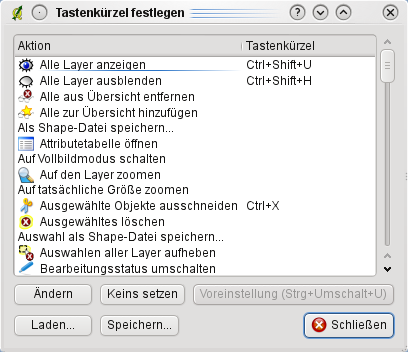
\includegraphics[clip=true, width=8cm]{shortcuts}
   \caption{Define shortcut options \nixcaption (KDE)} \label{fig:shortcuts}
\end{figure}

Configuration is very simple. Just select a feature from the list and click
on \button{Change}, \button{Set none} or \button{Set default}. Once you have
found your configuration, you can save it as XML file and load it to another
QGIS installation. 

\section{Rendering}\label{subsec:redraw_events}\index{rendering}

By default, QGIS renders all visible layers whenever the map canvas must be
refreshed. The events that trigger a refresh of the map canvas include:

\begin{itemize}
\item Adding a layer
\item Panning or zooming
\item Resizing the QGIS window
\item Changing the visibility of a layer or layers
\end{itemize}

QGIS allows you to control the rendering process in a number of ways.

\subsection{Scale Dependent Rendering}\index{rendering!scale dependent}
\label{label_scaledepend}

Scale dependent rendering allows you to specify the minimum and maximum
scales at which a layer will be visible.  To set scale dependency rendering,
open the \dialog{Properties} dialog by double-clicking on the layer in the 
legend. On the \tab{General} tab, set the minimum and maximum scale values and then
click on the \checkbox{Use scale dependent rendering} checkbox.

You can determine the scale values by first zooming to the level you want
to use and noting the scale value in the QGIS status bar.\index{scale}

\subsection{Controlling Map Rendering}\label{label_controlmap}

Map rendering can be controlled in the following ways:

\minisec{a) Suspending Rendering}\index{rendering!suspending}
\label{label_suspendrender}

To suspend rendering, click the \checkbox{Render} checkbox in the lower right
corner of the statusbar. When the \checkbox{Render} box is not checked, QGIS
does not redraw the canvas in response to any of the events described in
Section \ref{subsec:redraw_events}. Examples of when you might want to suspend
rendering include:

\begin{itemize}
\item Add many layers and symbolize them prior to drawing
\item Add one or more large layers and set scale dependency before drawing
\item Add one or more large layers and zoom to a specific view before drawing
\item Any combination of the above
\end{itemize}

Checking the \checkbox{Render} box enables rendering and causes and immediate
refresh of the map canvas.

\minisec{b) Setting Layer Add Option}\label{label_settinglayer}
\index{rendering!options}\index{layers!initial visibility}

You can set an option to always load new layers without drawing them. This
means the layer will be added to the map, but its visibility checkbox in the
legend will be unchecked by default. To set this option, choose
menu option \mainmenuopt{Settings} > \dropmenuopt{Options} and click on the
\tab{Rendering \& SVG} tab. Uncheck the \checkbox{By default new layers added
to the map should be displayed} checkbox. Any layer added to the map will be
off (invisible) by default.

%\minisec{Stopping Rendering}\index{rendering!halting}
%\label{label_stoprender}
%
%To stop the map drawing, press the ESC key. This will halt the refresh of
%the map canvas and leave the map partially drawn. It may take a bit of time
%between pressing ESC and the time the map drawing is halted.
%
%\textbf{NOTE}: It is currently not possible to stop rendering - this was disabled 
%in qt4 port because of User Interface (UI) problems and crashes.

\minisec{c) Updating the Map Display During Rendering}
\label{label_updatemap}\index{rendering!update during drawing}

You can set an option to update the map display as features are drawn. By
default, QGIS does not display any features for a layer until the entire
layer has been rendered. To update the display as features are read from the
datastore, choose menu option \mainmenuopt{Settings} > \dropmenuopt{Options}
click on the \tab{Rendering \& SVG} tab. Set the feature count to an
appropriate value to update the display during rendering. Setting a value of 0
disables update during drawing (this is the default). Setting a value too low
will result in poor performance as the map canvas is continually updated
during the reading of the features. A suggested value to start with is 500. 

\minisec{d) Influence Rendering Quality}
\label{label_renderquality}\index{rendering!quality}

To influence the rendering quality of the map you have 3 options. Choose menu 
option \mainmenuopt{Settings} > \dropmenuopt{Options} click on the 
\tab{Rendering \& SVG} tab and select or deselect following checkboxes.

\begin{itemize}
\item \checkbox{Make lines appear less jagged at the expense of some drawing
performance}
\item \checkbox{Fix problems with incorrectly filled polygons}
\end{itemize}

\section{Measuring}\label{sec:measure}\index{measure}

Measuring works within projected coordinate systems only (e.g., UTM). If 
the loaded map is defined with a geographic coordinate system
(latitude/longitude), the results from line or area measurements will be 
incorrect. To fix this you need to set an appropriate map coordinate system 
(See Section~\ref{label_projections}). Both measuring modules also use the 
snapping settings from the digitizing module. This is useful, if you want to 
measure along lines or areas in vector layers.  

\subsection{Measure length, areas and angles}
\index{measure:line length}
\index{measure:areas}
\index{measure:angles}


\includegraphics[width=0.7cm]{mActionMeasure} 
QGIS is also able to measure real distances between given 
points according to a defined ellipsoid. To configure this, choose menu option 
\mainmenuopt{Settings} > \dropmenuopt{Options}, 
click on the \tab{Map tools} tab and choose the appropriate ellipsoid. There
you can also define a rubberband color and your preferred measurement units
(meters or feet). The tool then allows you to click points on the map. Each
segment-length as well as the total shows up in the measure-window. To stop measuring click your right mouse button. \\

\includegraphics[width=0.7cm]{mActionMeasureArea} Areas can also be measured. 
In the measure window the accumulated area-size appears  \\
In addition, the measuring tool will snap to the currently selected layer, provided that layer has its snapping tolerance set. (See Section~\ref{snapping_tolerance}). So if you want to measure exactly along a line feature, or around a polygon feature, first set its snapping tolerance, then select the layer. Now, when using the measuring tools, each mouse click (within the tolerance setting) will snap to that layer. \\

\includegraphics[width=0.7cm]{mActionMeasureAngle}
You can also measure angles, selecting Measure Angle tool. The cursor becomes 
cross-shaped. Click to draw the first segment of the angle you wish to
measure, then move the the cursor to draw the desired angle. The measure
is displayed in a popup dialog. 
\begin{figure}[ht]
\centering
   \subfloat[Measure lines] {\label{subfig:measure_line}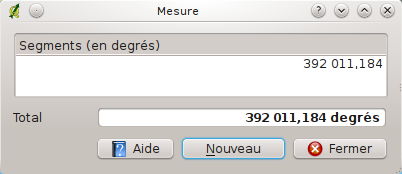
\includegraphics[clip=true, width=0.3\textwidth]{measure_line}}
     \hspace{1cm}
   \subfloat[Measure areas]{\label{subfig:measure_area}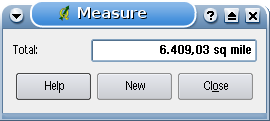
\includegraphics[clip=true, width=0.3\textwidth]{measure_area}}
   \caption{Measure tools in action \nixcaption} \label{fig:measure}
\end{figure}

\section{Projects}\label{sec:projects}\index{projects}

The state of your QGIS session is considered a Project.  QGIS
works on one project at a time.  Settings are either considered
as being per-project, or as a default for new projects (see
Section \ref{subsec:gui_options}). QGIS can save the state of your 
workspace into a project file using the menu options 
\mainmenuopt{File} > \dropmenuopttwo{mActionFileSave}{Save Project}
or \mainmenuopt{File} > \dropmenuopttwo{mActionFileSaveAs}{Save Project As}.

Load saved projects into a QGIS session using 
\mainmenuopt{File} > \dropmenuopttwo{mActionFileOpen}{Open Project}
or \mainmenuopt{File} > \dropmenuopt{Open Recent Project}.
If you wish to clear your session and start fresh, choose
\mainmenuopt{File} > \dropmenuopttwo{mActionFileNew}{New Project}.
Either of these menu options will prompt you to save the existing project
if changes have been made since it was opened or last saved.

The kinds of information saved in a project file include:

\begin{itemize}
\item Layers added
\item Layer properties, including symbolization
\item Projection for the map view
\item Last viewed extent
\end{itemize}

The project file is saved in XML format, so it is possible to edit
the file outside QGIS if you know what you are doing. The file format 
was updated several times compared to earlier QGIS versions. Project files 
from older QGIS versions may not work properly anymore. To be made aware of this, 
in the \tab{General} tab under \mainmenuopt{Settings} > \dropmenuopt{Options} 
you can select 

\checkbox{Promt to save project changes when required} \\
\checkbox{Warn when opening a project file saved with an older version of
QGIS}.

\minisec{Project Properties}
In the properties window for the project under \nix{\mainmenuopt{File} >
\dropmenuopt{Project Properties}} or \win{\mainmenuopt{Settings} >
\dropmenuopt{Project Properties}} you set project specific options. These
include:

\begin{itemize}
\item In the \tab{General} tab the project title, selection and background
color, layer units, precision, and the option to save relative paths to
layers can be defined. In addition the topological editing, and layerwise 
snapping options are set here.
\item The \tab{CRS} Coordinate Reference System tab enables you to choose the
CRS for this project, and to enable on-the-fly reprojection of vector layers
when displaying layers from a different CRS.
\item With the third \tab{Identifiable layers} tab you set (or disable) which
layers will respond to the identify tool. (See the Map tools paragraph from
the \ref{subsec:gui_options} section to enable identifying of multiple layers.)
\end{itemize}
 
\section{Output}\label{sec:output}
\index{output!save as image!print composer!quick print}

There are several ways to generate output from your QGIS session. We have
discussed one already in Section \ref{sec:projects}: saving as a project file. 
Here is a sampling of other ways to produce output files:

\begin{itemize}
\item Menu option \dropmenuopttwo{mActionSaveMapAsImage}{Save as Image} opens
a file dialog where you select the name, path and type of image (PNG or JPG
format). A world file with extension PNGW or JPGW saved in the same folder
georeferences the image.
\item Menu option \dropmenuopttwo{mActionFilePrint}{Print Composer} opens a
dialog where you can layout and print the current map canvas (see
Section~\ref{label_printcomposer}).
\item The \toolbtntwo{quick_print}{Quick Print} plugin allows
to print a simple map with minimal effort (see Section \ref{quickprint}).
\end{itemize}

\section{GUI Options}\label{subsec:gui_options}


\includegraphics[width=0.7cm,clip=true]{mActionOptions} Some basic options
for QGIS can be selected using the \dialog{Options} dialog. Select the 
menu option \mainmenuopt{Settings} >
\dropmenuopttwo{mActionOptions}{Options}. The tabs where you can 
optmize your options are:

\minisec{General Tab}

\begin{itemize}
\item \checkbox{Promt to save project changes when required}
\item \checkbox{Warn when opening a project file saved with an older version of QGIS}
\item Change Selection and backgroud Color
\item Change the icon theme (choose between default, classic, gis and nkids)
\item \checkbox{Capitalise layer names in legend}
\item \checkbox{Display classification attribute names in legend}
\item \checkbox{Hide splash screen at startup}
\item \checkbox{Open identify results in a dock window (QGIS restart
required)}
\item \checkbox{Open attribute table in a dock window}
\item \checkbox{Add PostGIS layers with double click and select in extended mode}
% \item Define attribute table behavior (choose between show all features, show
% selected features and show features in current canvas)
\end{itemize}

\minisec{Rendering \& SVG Tab}

\begin{itemize}
\item \checkbox{By default new layers added to the map should be displayed}
\item Define number of features to draw before updating the display.
\item \checkbox{Use render caching where possible to speed up redraws}
\item \checkbox{Make lines appear less jagged at the expense of some drawing
performance}
\item \checkbox{Fix problems with incorrectly filled polygons}
\item \checkbox{Use new generation symbology for rendering}
\item Add and remove path(s) to search for Scalable Vector Graphics (SVG)
symbols
\end{itemize}

\minisec{Map tools Tab}

\begin{itemize}
\item The Mode setting determines which layers will be shown by the Identify
tool. By switching to \usertext{Top down} or \usertext{Top down, stop at
first} instead of \usertext{Current layer} attributes for all identifiable
layers (see the Project properties section under: \ref{sec:projects} to set
which layers are identifiable) will be shown with the Identify tool.
\item \checkbox{Open feature form, if a single feature is identified}
\item Define search radius as a percentage of the map width
\item Define ellipsoid for distance calculations
\item Define rubberband color for measure tools
\item Define preferred measurement units (meters or feet)
\item Define Mouse wheel action (Zoom, Zoom and recenter, Zoom to mouse
cursor, Nothing)
\item Define Zoom factor for wheel mouse
\end{itemize}

\minisec{Overlay}

\begin{itemize}
\item Define placement algorithm for labels (choose between central point
(standard), chain, popmusic tabu chain, popmusic tabu and popmusic chain)
\end{itemize}

\minisec{Digitizing Tab}

\begin{itemize}
\item Define Rubberband Color and line width for Digitizing
\item Define default snap mode (to vertex, to segment, to vertex and segment)
\item Define default snapping tolerance in map units or pixel
\item Define search radius for vertex edits in map units or pixel
\item \checkbox{Show markers only for selected features}
\item Define vertex marker style (Cross, semi transparent circle or none) and
size
\item \checkbox{Suppress attributes pop-up windows after each created feature}
\end{itemize}

\minisec{CRS Tab}

\begin{itemize}
\item \checkbox{Prompt for Coordinate Reference System (CRS)}
\item \checkbox{Project wide default Coordinate Reference System (CRS) will be used}
\item \checkbox{Global default Coordinate Reference System (CRS) displayed below will be used}
\item Select global default Coordinate Reference System (CRS)
\end{itemize}

\minisec{Locale Tab}

\begin{itemize}
\item \checkbox{Overwrite system locale and use defined locale instead}
\item Information about active system locale
\end{itemize}

\minisec{Proxy Tab}

\begin{itemize}
\item \checkbox{Define timeout for network requests in ms}
\item \checkbox{Use proxy for web access} and define host, port, user, and password.
\item Set the \dropmenuopt{Proxy type} according to your needs
 \begin{itemize}
  \item \dropmenuopt{Default Proxy}: Proxy is determined based on the application proxy set using
  \item \dropmenuopt{Socks5Proxy}: Generic proxy for any kind of connection. Supports TCP, UDP, binding to a port (incoming connections) and authentication.
  \item \dropmenuopt{HttpProxy}: Implemented using the "CONNECT" command, supports only outgoing TCP connections; supports authentication.
  \item \dropmenuopt{HttpCachingProxy}: Implemented using normal HTTP commands, it is useful only in the context of HTTP requests
  \item \dropmenuopt{FtpCachingProxy}: Implemented using an FTP proxy, it is useful only in the context of FTP requests
 \end{itemize}
\end{itemize}

Excluding some URLs can be added to the textbox below the proxy-settings (see
fig. \ref{fig:proxy-settings}) by pressing the \button{Add}-button. After that
double-click into the just created URL-field and enter the URL you would like
to exclude from using the proxy. Obviously the button \button{Remove} removes the selected
entry.

If you need more detailed information about the different proxy-settings,
please refer to the manual of the unterlaying QT-library-documentation at
\url{http://doc.trolltech.com/4.5/qnetworkproxy.html#ProxyType-enum}.

\begin{figure}[ht]
   \centering
   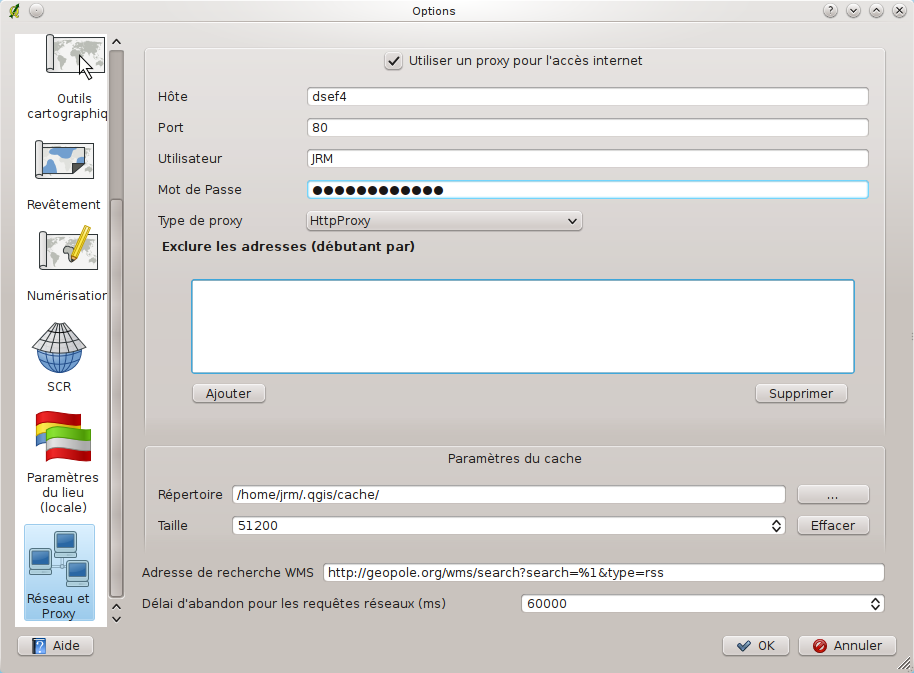
\includegraphics[clip=true, width=10cm]{proxy-settings}
   \caption{Proxy-settings in \qg \nixcaption}
   \label{fig:proxy-settings}
 
\end{figure}

\begin{Tip} \caption{\textsc{Using Proxies}}
Using proxies can sometimes be tricky. It is useful to 'trial and
error' the above proxy types and check if they succeed in your case.
\end{Tip}

You can modify the options according to your needs. Some of the changes may 
require a restart of QGIS before they will be effective.

\begin{itemize}
\item \nix{settings are saved in a texfile: \$HOME/.config/QuantumGIS/qgis.conf}
\item \osx{you can find your settings in: \$HOME/Library/Preferences/org.qgis.qgis.plist}
\item \win{settings are stored in the registry under:}
\begin{verbatim}
\\HKEY\CURRENT\USER\Software\QuantumGIS\qgis
\end{verbatim}
\end{itemize}


\section{Spatial Bookmarks}\label{sec:bookmarks}
\index{bookmarks}
\index{spatial bookmarks|\see{bookmarks}}

Spatial Bookmarks allow you to ``bookmark'' a geographic location and return to it later.

\subsection{Creating a Bookmark}
To create a bookmark:
\begin{enumerate}
\item Zoom or pan to the area of interest.
\item Select the menu option \mainmenuopt{View} > \dropmenuopt{New Bookmark} or press \keystroke{Ctrl-B}.
\item Enter a descriptive name for the bookmark (up to 255 characters).
\item Click \button{OK} to add the bookmark or \button{Cancel} to exit without adding the bookmark.
\end{enumerate}

Note that you can have multiple bookmarks with the same name.

\subsection{Working with Bookmarks}
To use or manage bookmarks, select the menu 
option \mainmenuopt{View} > \dropmenuopt{Show Bookmarks}.
The \dialog{Geospatial Bookmarks} dialog allows you to zoom to or delete a bookmark.
You can not edit the bookmark name or coordinates.

\subsection{Zooming to a Bookmark}
From the \dialog{Geospatial Bookmarks} dialog, select the desired bookmark by clicking on it, 
then click \button{Zoom To}.
You can also zoom to a bookmark by double-clicking on it.

\subsection{Deleting a Bookmark}
To delete a bookmark from the \dialog{Geospatial Bookmarks} dialog, click on it then click
 \button{Delete}.
Confirm your choice by clicking \button{Yes} or cancel the delete by clicking \button{No}.

\FloatBarrier

% vim:autoindent:set textwidth=78:
% !TeX root = user_guide.tex

\chapter{Arbeiten mit Vektordaten}
\label{label_workingvector}
\index{Vektorlayer|(}

% when the revision of a section has been finalized,
% comment out the following line:
% \updatedisclaimer

QGIS benutzt die OGR-Bibliothek, um Vektorformate zu lesen und zu schreiben,
\footnote{GRASS Vektor und PostgreSQL Support wird durch native Datenprovider 
Plugins bereitgestellt.} wie etwa das ESRI Shape,\index{Shapedateien}\
index{ESRI!Shapedateien}\index{SHP Dateien} MapInfo MIF (Austauschformat)
\index{MIF Dateien}\index{MapInfo!MIF Dateien} und MapInfo TAB 
(Natives Format).\index{TAB Dateien}\index{MapInfo!TAB Dateien}. Derzeit werden 
etwa 60 Vektorformate unterst�tzt. Eine komplette Liste finden Sie unter der 
URL: \url{http://www.gdal.org/ogr/ogr_formats.html}.

\textbf{Note}: Einige der aufgelisteten Formate k�nnen auf ihrem Rechner aus unterschiedlichen Gr�nden nicht unterst�tzt werden. Einige brauchen z.B. 
kommerzielle Bibliotheken oder die GDAL Installation auf Ihrem Rechner, wurde 
ohne die Unterst�tzung f�r das entsprechende Format erstellt. Nur Formate, die 
getestet wurden, k�nnen ausgew�hlt werden, wenn Sie eine Vektordatei in QGIS 
laden. Alle anderen werden angezeigt, wenn Sie *.* ausw�hlen.

Das Arbeiten mit GRASS GIS Vektorlayern bildet an manchen Stellen eine Ausnahme
und wird daher in Kapitel \ref{sec:grass} explizit beschrieben.

In diesem Abschnitt wird beispielhaft beschrieben, wie man mit ESRI Shapes,
PostGIS- und SpatiaLite-Layern arbeitet. Viele Funktionen in QGIS sind
unabh�ngig vom verwendeten Datenformat und verhalten sich daher identisch. Dies 
ist gewollt und bezieht sich u.a. auf Abfrage, Selektion, Beschriftung und 
Attributfunktionen.

\section{ESRI Shapes}
\index{Vektorlayer!ESRI Shapedateien}
\index{Shapedateien}
\index{ESRI!Shapedateien}
\index{SHP Dateien}

ESRI Shape ist das Standard Vektorformat in QGIS und wird durch die OGR Simple
Feature Library \url{http://www.gdal.org/ogr}\index{OGR} bereitgestellt.
Ein Shape besteht aus mindestens drei Dateien:\index{Shapedateien!Format}

\begin{itemize}[label=--]
\item .shp Datei (enth�lt die Geometrien)
\item .dbf Datei (enth�lt die Attribute im dBase-Format)
\item .shx Datei (enth�lt den r�umlichen Index)
\end{itemize}

Dar�berhinaus kann eine Datei mit .prj Endung existieren. Diese enth�lt
die Projektionsinformationen des Shapes. Es k�nnen noch weitere Dateien zu
einem Shape geh�ren. Details dazu finden sich in der technischen
Spezifikation unter \\
\url{http://www.esri.com/library/whitepapers/pdfs/shapefile.pdf}
\index{Shapedateien!Spezifikation}.

\minisec{Problem beim Laden eines Shapes mit .prj Datei}

Wenn Sie ein Shape mit \filename{.prj} Datei laden und QGIS ist nicht in 
der Lage, die Projektionsinformationen korrekt auszulesen, ist es notwendig 
das Koordinatenbezugsystem (KBS) manuell im \tab{Allgemein} Reiter des 
\dialog{Layereigenschaften} Dialog anzugeben. Hintergrund ist, dass 
\filename{.prj} Dateien oftmals nich die vollst�ndigen Projektionsparameter 
enthalten, so wie QGIS sie ben�tigt und auch im \dialog{KBS} Dialog anzeigt.

Aus diesem Grund, wenn Sie ein neues Shapefile mit QGIS erstellen, werde 
derzeit zwei unterschiedliche Projektionsdateien angelegt. Eine \filename{.prj} 
Datei, mit den unvollst�ndigen Projektionsparameters, wie sie z.B. von ESRI 
Software gelesen und erstellt wird, und eine \filename{.qpj} Datei, in der die 
vollst�ndigen Projektionsparameter anthalten sind. Wenn Sie dann ein Shape in 
laden, und QGIS findet eine \filename{.qpj} Datei, dann wird diese anstelle 
der \filename{.prj} Datei benutzt. \index{Shapedateien!Spezifikationen}

\subsection{Shape Layer laden}\label{sec:load_shapefile}

\begin{figure}[ht]
   \begin{center}
   \caption{Dialogfenster zum Laden OGR-unterst�tzter Layer \nixcaption}\label{fig:addvectorlayer}\smallskip
   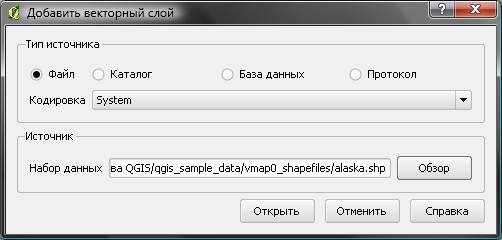
\includegraphics[clip=true, width=12cm]{addvectorlayerdialog}
\end{center}
\end{figure}


\includegraphics[width=0.7cm]{mActionAddNonDbLayer} Um ein Shape zu laden,
starten Sie QGIS und klicken auf das Icon
\toolbtntwo{mActionAddNonDbLayer}{Vektorlayer hinzuf�gen} in der
Werkzeugleiste\index{Shapedateien!�ffnen} oder mit der Taste 
\keystroke{Strg-Shift-V}. Mit demselben Tool k�nnen Sie auch alle anderen 
durch OGR unterst�tzten Formate laden.

W�hlen Sie aus den m�glichen Quelltypen \radiobuttonon{Datei} und klicken Sie
auf den Knopf \button{Durchsuchen}. Dadurch erscheint ein weiterer Dialog zum
�ffnen eines OGR-Vektorlayers (siehe Abbildung~\ref{fig:openshapefile}), mit
dessen Hilfe Sie in Ihrem Dateisystem navigieren und die entsprechenden zu
ladenden Dateien ausw�hlen k�nnen. Die Auswahlbox \selectstring{Dateien des
Typs}{\ldots} erm�glicht es, im Vorfeld ein Dateiformat auszuw�hlen. 

Au�erdem kann auch der Kodierungstyp f�r das Shape eingestellt werden, falls
dies notwendig ist.  

\begin{figure}[ht]
   \begin{center}
   \caption{Dialogfenster zum Auswahlen eines Vektorlayers \nixcaption}\label{fig:openshapefile}\smallskip
   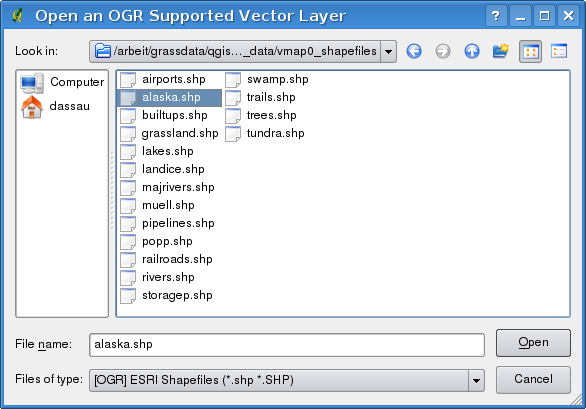
\includegraphics[clip=true, width=12cm]{shapefileopendialog}
\end{center} 
\end{figure}

Durch Auswahl eines Shapes und Anklicken des Knopfes \button{�ffnen} wird die
Datei in QGIS geladen. In Abbildung~\ref{fig:loadedshapefile} sehen Sie das Ergebnis,
nachdem die Beispieldatei \filename{alaska.shp} geladen wurde.

\begin{figure}[ht]
   \begin{center}
   \caption{QGIS mit einem geladenen Alaska Shape \nixcaption}\label{fig:loadedshapefile}\smallskip
   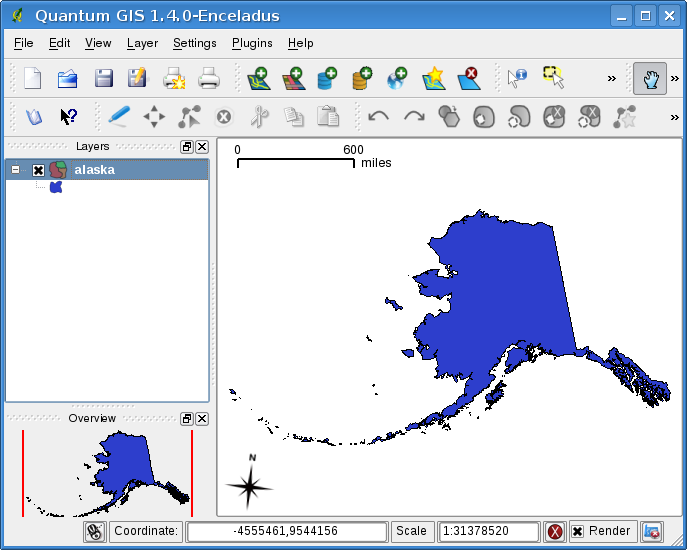
\includegraphics[clip=true, width=\textwidth]{shapefileloaded}
\end{center} 
\end{figure}

\begin{Tip}\caption{\textsc{Farben von Vektorlayern}}
Wenn Sie einen neuen Vektorlayer in QGIS laden, werden Farben
zuf�llig zugewiesen. Wenn Sie mehrere neue Vektorlayer laden, werden jeweils
unterschiedliche Farben zugewiesen.
\end{Tip}

Nach dem Laden k�nnen Sie mit den Navigationstools aus der Werkzeugleiste
beliebig zoomen oder den Layer verschieben. Um den
\dialog{Eigenschaften}-Dialog eines Vektorlayers zu �ffnen, doppelklicken Sie
auf den Layernamen in der Legende oder zeigen Sie mit der Maus auf den
Layernamen, dr�cken Sie die rechte Maustaste und w�hlen
\dropmenuopt{Eigenschaften}. Vergleichen Sie Abschnitt~\ref{sec:symbology}
f�r weitere Informationen zum Editieren der Eigenschaften von Vektorlayern.

\begin{Tip}\caption{\textsc{Layer und Projekte von externen Datentr�gern laden
unter OS X}}
Unter OS X werden externe Datentr�ger unter Datei \arrow �ffne Projekt
nicht gemeinsam mit den internen Festplatten angezeigt. Dies soll zuk�nftig
behoben werden. Solange k�nnen Sie '/Volumes' in das Eingabefenster
'Dateiname' eintragen und return dr�cken. Danach k�nnen Sie auch zu den
externen Datentr�gern bzw. Rechnern in einem Netzwerk browsen.
\end{Tip}
 
\subsection{Darstellungsgeschwindigkeit optimieren}

Um die Darstellungsgeschwindigkeit zu optimieren, kann ein r�umlicher Index
erstellt werden. Ein\index{R�umlicher Index!Shapedateien} r�umlicher Index
erh�ht die Geschwindigkeit beim Zoomen und Verschieben. R�umliche Indizes
haben in QGIS die Endung \filename{.qix}.

Benutzen Sie folgende Schritte zum Erstellen eines r�umlichen Index:

\begin{itemize}[label=--]
\item Laden Sie ein Shape
\item �ffnen Sie den \dialog{Eigenschaften}-Dialog des Vektorlayers, indem
Sie auf den Namen des Layers in der Legende doppelklicken oder mit der
rechten Maustaste \dropmenuopt{Eigenschaften} ausw�hlen. 
\item In dem Reiter \tab{Allgemein} klicken Sie auf den \button{Erstellen}-Knopf
im Bereich \button{R�umlichen Index erstellen}
\end{itemize}

\section{MapInfo Layer laden}
\index{Vektorlayer!MapInfo}

Um eine MapInfo Datei zu laden, klicken Sie auf das Icon
\toolbtntwo{mActionAddNonDbLayer}{Vektorlayer hinzuf�gen} in der
Werkzeugleiste oder dr�cken Sie die Taste \keystroke{Strg-Shift-V}. W�hlen Sie 
aus den m�glichen Quelltypen \radiobuttonon{Datei} und klicken Sie auf den Knopf
\button{Durchsuchen}. Definieren Sie unter \selectstring{Dateien des
Typs}{MapInfo (*.mif *.tab *.MIF *.TAB)} und w�hlen die gew�nschte Datei aus.

\subsection{ArcInfo Binary Coverage laden}
\index{Vektorlayer!ArcInfo Coverage}

Um ein ArcInfo Coverage zu laden, klicken Sie auf das Icon
\toolbtntwo{mActionAddNonDbLayer}{Vektorlayer hinzuf�gen} in der
Werkzeugleiste oder dr�cken Sie die Taste \keystroke{Strg-Shift-V}. W�hlen Sie 
aus den m�glichen Quelltypen \radiobuttonon{Verzeichnis}, w�hlen Sie als
\selectstring{Typ}{ArcInfo Binary Coverage} und klicken Sie auf den Knopf
\button{Durchsuchen}. W�hlen Sie nun den Ordner mit den ArcInfo Binary
Coverage Dateien aus, in der sich beispielweise folgende Dateien befinden
k�nnen:  

\begin{itemize}[label=--]
\item .lab - Attributlayer laden (Fl�chenattribute oder Punktdaten)
\item .cnt - Polygon-Centroid-Layer laden
\item .arc - Linienlayer laden
\item .pal - Polygonlayer laden
\end{itemize}

Klicken Sie auf \button{Ok}. Es �ffnet sich jetzt ein weiterer Dialog mit
einer Liste der vorhandenen Unterlayer, die sich in dem ausgew�hlten Ordner
befinden. W�hlen Sie die gew�nschten Layer aus und klicken Sie wieder auf
\button{Ok}, um diese in QGIS anzuzeigen.

Auf die gleiche Art und Weise k�nnen auch andere Verzeichnis-basierte
Vektorlayer geladen werden, wie etwa das U.K. National Transfer Format, das
raw TIGER Format des U.S. Census Bureau oder auch GRASS Vektorlayer. Letztere
werden normalerweise aber �ber das GRASS Plugin geladen (siehe
Kapitel~\ref{sec:grass}).

\section{PostGIS Layer laden}
\index{Vektorlayer!PostGIS}
\index{PostGIS!Layer}
\label{label_postgis} 

PostGIS-Ebenen sind in einer PostgreSQL Datenbank gespeichert. Der Vorteil
von PostGIS liegt in der F�higkeitkeit, r�umliche Indizes, Filterungen und
Abfragen bereitszustellen. Vektorfunktionen wie Selektieren und Abfragen
funktionieren besser als bei Ebenen, die durch die OGR-Bibliothek geladen
wurden.

\subsection{Erstellen einer PostGIS Anbindung}\index{PostgreSQL!Verbindung}\label{sec:postgis_stored}

Beim ersten Einbinden einer PostGIS-Datenbank muss eine Anbindung erstellt
und gespeichert werden.
Klicken Sie dazu auf das Icon \toolbtntwo{mActionAddLayer}{PostGIS-Layer
hinzuf�gen} in der Werkzeugleiste oder aus dem Men� \mainmenuopt{Layer}. 
Der \texttt{PostGIS Tabelle(n) hinzuf�gen}-Dialog erscheint daraufhin. Um
eine neue Anbindung zu erstellen, klicken Sie auf den Knopf \button{Neu}.
Sie k�nnen dazu auch auf das Icon \toolbtntwo{mActionAddNonDbLayer}{Vektorlayer
hinzuf�gen} klicken, und aus den m�glichen Quelltypen
\radiobuttonon{Datenbank} ausw�hlen und dann auf den Knopf \button{Neu}
dr�cken. Der Dialog \dialog{Neue PostGIS-Verbindung erzeugen} �ffnet sich,
und Sie k�nnen die notwendigen Parameter aus Tabelle
\ref{tab:postgis_connection_parms} eingeben und speichern.

\begin{table}[h]\index{PostgreSQL!Verbindungsparameter}
\centering
\caption{PostGIS Verbindungsparameter}\label{tab:postgis_connection_parms}\medskip
 \begin{tabular}{|l|p{5in}|}
\hline Name & Ein Name f�r die Verbindung. Kann derselbe wie f�r die
Datanbank sein \\
\hline Service & Service Parameter, der anstelle von Host / Port und potenziell 
auch Datenbank verwendet werden kann. Kann unter pg\_service.conf definiert werden. \\
\hline Host \index{PostgreSQL!Host} & Name des Datenbank-Hosts. Dies muss ein
aufl�sbarer Name f�r den HOST sein, genau wie beim Benutzen von telnet oder ping \\
\hline Port \index{PostgreSQL!Port}& Port Nummer der Datenbank auf dem
Server. Standard ist 5432.\\
\hline Datenbank \index{PostgreSQL!Datenbank} & Name der Datenbank  \\
\hline SSL Modus \index{PostgreSQL!SSL Modus}& Wie die SSL-Verbindung mit dem
Server festgelegt wird. Die Optionen sind:
\begin {itemize}
\item abschalten: Versuche nur eine Nicht-SSL-Verbindung.
\item erlauben: Versuche eine Nicht-SSL-Verbindung. Wenn das nicht
klappt, versuche eine SSL-Verbindung.
\item bevorzugen (the default): Versuche eine SSL-Verbindung. Wenn das nicht
klappt, versuche eine Nicht-SSL-Verbindung;
\item verlangen: Versuche nur eine SSL-Verbindung.
\end {itemize}
Bemerkung: Die Geschwindigkeit der Verbindung kann oftmals enorm gesteigert
werden, wenn die SSL-Verbindung abgeschaltet wird. \\
\hline Benutzername \index{PostgreSQL!Benutzername}& Benutzername, um sich bei
der Datenbank anzumelden \\
\hline Passwort \index{PostgreSQL!Passwort}& Passwort, um sich als
\filename{Benutzer} mit der Datenbank zu verbinden\\
\hline
\end{tabular}
\end{table}

Optional k�nnen noch die folgenden Kontrollk�stchen aktiviert werden:

\begin{itemize}[label=--]
\item \checkbox{Benutzernamen speichern}
\item \checkbox{Passwort speichern}
\item \checkbox{Nur in geometry\_columns nachschauen}
\item \checkbox{Nur im 'public' Schema nachschauen}
\item \checkbox{Auch geometrielose Tabellen anzeigen}
\item \checkbox{Gech�tzte Tabellenmetadaten nutzen}
\end{itemize}

Wenn alle Parameter eingetragen sind, kann die Verbindung getestet werden,
indem Sie auf den Knopf \button{Verbindung testen} 
dr�cken\index{PostgreSQL!Verbindung!Testen}. 

\begin{Tip}\caption{\textsc{QGIS Benutzereinstellungen und Sicherheit}}
\index{Einstellungen}\index{Sicherheit} 
Ihre Einstellungen f�r QGIS werden
abh�ngig von Ihrem Betriebssystem gespeichert. Unter \nix ist dies in Ihrem
Homeverzeichnis unter .qt/qgisrc. Unter \win ist es in der Registry. Abh�ngig
von Ihrer Arbeitsumgebung kann das Speichern von Passworten in den
QGIS-Einstellungen ein Sicherheitsrisiko darstellen.
\end{Tip}

\minisec{Laden eines Layers aus der PostGIS Datenbank}\index{PostgreSQL!Layer
laden}

Nachdem Sie eine oder mehrere Verbindungen definiert und gespeichert haben,
k�nnen Sie einzelne Ebenen aus PostGIS laden. Nat�rlich brauchen Sie dazu
Daten in PostgreSQL/PostGIS. Eine Beschreibung zum Import von Daten nach
PostgreSQL/PostGIS lesen Sie Abschnitt \ref{sec:loading_postgis_data}.

Um eine Ebene aus PostGIS zu laden, f�hren Sie folgende Schritte durch:

\begin{itemize}[label=--]
\item Wenn der \dialog{PostGIS Tabelle(n) hinzuf�gen}-Dialog noch nicht
ge�ffnet ist, klicken Sie auf den Knopf
\toolbtntwo{mActionAddLayer}{PostGIS-Layer hinzuf�gen} in der Werkzeugleiste
\item W�hlen Sie eine Verbindung aus dem Drop-Down Men� und klicken auf
\button{Verbinden}
\item W�hlen Sie \checkbox{Auch geometrielose Tabellen anzeigen} an oder ab.
\item Optional aktivieren Sie den Bereich \checkbox{Suchoptionen}, um eine 
Auswahl anzuzeigender Objekte zu treffen.
\item Suchen Sie einen Layer, den Sie laden m�chten
\item W�hlen Sie den Layer durch doppelklicken aus. Sie k�nnen mehrere Ebenen
ausw�hlen, indem Sie die \keystroke{Umschalt}-Taste beim Ausw�hlen gedr�ckt
halten. Weitere Informationen, z.B. zum Umgang mit dem PostgreSQL
Query-Builder finden Sie in Abschnitt~\ref{sec:query_builder}.
\item Klicken Sie auf den Knopf \button{Hinzuf�gen}, um den Layer zu laden.
\end{itemize}

\begin{Tip}\caption{\textsc{PostGIS-Layer}}
Normalwerweise ist ein PostGIS-Layer �ber einen Eintrag in der
geometry\_columns Tabelle definiert. Seit Version 0.9.0 ist QGIS in der Lage,
Layer zu laden, die keinen Eintrag in der geometry\_columns Tabelle
besitzen. Dies bezieht sich auf Tabellen und Views. Um einen 'spatial view' zu
definieren, brauchen Sie ein kraftvolles System, um die Daten zu
visualisieren. Beziehen Sie sich auf das PostgreSQL Handbuch, um weitere
Informationen �ber die Erstellung von Views zu erhalten.
\end{Tip}

\subsection{Einige Details zu PostGIS-Layern}\label{sec:postgis_details}
\index{PostgreSQL!Layerdetails}

Dieser Abschnitt enth�lt einige Details, wie QGIS auf PostgreSQL zugreift.
Meistens soll QGIS eine Liste mit ein paar Datenbanktabellen bereitstellen,
die bei Bedarf geladen werden k�nnen. Wenn Sie Probleme mit dem Laden von
Layern aus PostgreSQL haben, k�nnen die nun folgenden Informationen
vielleicht eine Hilfe sein, die Fehlermeldungen von QGIS besser zu verstehen
und eine L�sung zu finden, die PostgreSQL Tabellen- oder Viewdefinition
anzupassen, und somit den Layer laden zu k�nnen.

QGIS braucht eine Spalte in der PostgreSQL Tabelle, die als eindeutiger
Schl�ssel f�r den Layer genutzt werden kann. F�r Tabellen bedeutet dies, dass
die Tabelle normalerweise einen Prim�rschl�ssel braucht oder eine Spalte mit
eindeutiger Zuordnung. F�r QGIS muss diese Spalte au�erdem vom Typ int4 sein
(Integer mit 4 Bytes). Als Alternative kann auch die Spalte ctid als
Prim�rschl�ssel-Spalte verwendet werden. Wenn eine Tabelle diese
Voraussetzungen nicht erf�llt, wird die oid-Spalte genutzt. Die
Performanz steigt, wenn f�r die Spalte ein Index erstellt wurde (f�r
Prim�rschl�ssel wird in PostgreSQL automatisch ein Index erstellt).

Wenn der PostGIS-Layer ein View ist, gelten dieselben Anforderungen, aber
Views besitzen keinen Prim�rschl�ssel oder Spalten mit eindeutiger Zuordnung.
In diesem Fall wird QGIS versuchen, eine passende Spalte zu finden, die aus
der Tabellenspalte erstellt wurde. Dies geschieht, indem die View Definition
SQL-basiert durchsucht wird. Aber es gibt auch einige Aspekte der SQL, die
von QGIS ignoriert werden. Dies beinhaltet zum Beispiel die Verwendung von
Tabellen Aliases und Spalten, die durch SQL Funktionen generiert wurden. Wenn
so eine Prim�rschl�ssel Spalte nicht existiert, wird die Ebene nicht geladen.
In diesem Fall ist eine L�sung, den View anzupassen,
damit er eine entsprechende Spalte vom Typ int4 enth�lt, entweder mit einem
Prim�rschl�ssel oder eindeutiger Zuordnung und bevorzugt nat�rlich mit Index.

\subsection{Layer nach PostgreSQL/PostGIS importieren}\label{sec:loading_postgis_data}
\index{PostGIS!SPIT!Daten importieren}

\minisec{shp2pgsql}
Layer k�nnen auf unterschiedliche Art nach PostGIS importiert werden.
PostGIS selbst stellt ein Tool \filename{shp2pgsql} bereit, das genutzt
werden kann, um Shapes nach PostGIS zu importieren. Um ein Shape mit dem
Namen \filename{alaska.shp} in eine PostgreSQL/PostGIS Datenbank zu
importieren, wird folgendes Kommando benutzt:

\begin{verbatim} 
  shp2pgsql -s 2964 alaska.shp alaska_new | psql gis_data
\end{verbatim}

Dieser Befehl erzeugt eine neue Tabelle mit dem Namen \usertext{alaska\_new}
in der PostgreSQL/PostGIS Datenbank \usertext{gis\_data}. Die neue Ebene wird
die ID 2964 als 'spatial reference identifier' (SRID) tragen. Weitere
Informationen zu r�umlichen Referenzsystemen finden Sie in Abschnitt
\ref{label_projections}.

\begin{Tip}
\caption{\textsc{PostGIS-Layer exportieren}\index{PostGIS!Exportieren}}
Entsprechend dem Importtool \usertext{shp2pgsql} gibt es auch ein
Exporttool, um Daten von PostGIS ins Shape-Format zu exportieren:
\usertext{pgsql2shp}. Dieses Tool ist in der PostGIS-Installation enthalten.
\end{Tip}

\minisec{SPIT Plugin}

QGIS bietet ein Plugin mit dem Namen SPIT (Shapefile to PostGIS Import
Tool)\index{PostGIS!SPIT}. SPIT kann dazu
benutzt werden, gleichzeitig mehrere Shapes zu laden und bietet dabei auch
Support f�r Schemas. Um das Plugin zu benutzen, �ffnen Sie
\dropmenuopttwo{mActionShowPluginManager}{Plugins verwalten} im Men�
\mainmenuopt{Plugins}, w�hlen das \checkbox{SPIT} aus und dr�cken auf
\button{OK}. Das SPIT-Icon wird nun in der Plugin-Werkzeugleiste
angezeigt\index{PostGIS!SPIT!laden}.

Klicken Sie nun auf das \toolbtntwo{spiticon}{SPIT}-Icon in der
Werkzeugleiste, um den Dialog \dialog{Shapefile nach PostGIS Import Tool} zu
�ffnen. W�hlen Sie �ber den Knopf \button{Verbinden} eine PostGIS Datenbank
aus, definieren Sie ein paar Importparameter, wenn Sie m�chten. F�gen Sie 
dann mit dem Knopf \button{Hinzuf�gen} ein oder mehrere Shapes zu der Liste 
hinzu und klicken dann f�r den Import auf den Knopf \button{OK}. Der 
Fortschritt des Imports sowie Warnungen oder Fehlermeldungen werden f�r 
jedes Shape angezeigt.

\begin{Tip}\caption{\textsc{Shapes mit f�r PostgreSQL reservierten
Ausdr�cken importieren}}\index{PostGIS!SPIT!reservierte Ausdr�cke}
Wenn Sie ein Shape in der Liste zu importierender Daten haben,
welches Felder mit f�r PostgreSQL reservierten Ausdr�cken enth�lt, erscheint
ein Popup mit dem jeweiligen Status der Felder. Sie k�nnen die Namen der Felder
\index{PostGIS!SPIT!Spaltennamen editieren} dann vor dem Import editieren und
anpassen. Der Versuch die Datei ohne �nderung zu importieren, wird sehr
wahrscheinlich fehlschlagen.
\end{Tip}

\minisec{ogr2ogr}

Abgesehen von \filename{shp2pgsql} und \filename{SPIT} gibt es noch ein weiteres
Tool, um Daten nach PostGIS zu importieren: \filename{ogr2ogr}. Dieses Tool ist
Teil der GDAL-Installation. Um ein Shape nach PostGIS zu importieren, kann
folgendes Kommando verwendet werden:

\begin{verbatim}
  ogr2ogr -f "PostgreSQL" PG:"dbname=postgis host=myhost.de user=postgres \
  password=topsecret" alaska.shp
\end{verbatim}

Damit wird das Shape \filename{alaska.shp} vom Benutzer \usertext{postgres}
mit dem Passwort \usertext{topsecret} in die PostGIS Datenbank
\usertext{postgis} auf dem Server \usertext{myhost.de} importiert.

Wichtig ist, dass GDAL mit PostgreSQL-Support kompiliert sein muss, damit der
Import nach PostGIS m�glich ist. Dies kann mit folgendem Kommando getestet werden:

\begin{verbatim}
ogrinfo --formats | grep -i post
\end{verbatim}

Wenn Sie das PostgreSQL's Kommando \filename{COPY} anstatt der
Standardmethode \filename{INSERT INTO} verwenden m�chte, m�ssen Sie vorher
die folgende Variable exportieren (verifiziert unter \nix und \osx):

\begin{verbatim}
  export PG_USE_COPY=YES
\end{verbatim}

Der Befehl \filename{ogr2ogr} erstellt im Gegensatz zu \filename{shp2pgsl}
keinen r�umlichen Index. In diesem Fall m�ssen Sie ihn nachtr�glich manuell
erstellen mit dem SQL-Kommando \usertext{CREATE INDEX}. Die Schritte werden
im folgenden Kapitel~\ref{label_improve} n�her beschrieben.

\subsection{Geschwindigkeit optimieren} \label{label_improve}

Der Datentransfer von einer PostgreSQL/PostGIS Datenbank kann langsam sein,
besonders �ber ein Netzwerk. Die Geschwindigkeit kann optimiert werden, indem
f�r alle Ebenen in PostgreSQL ein r�umlicher Index\index{PostGIS!R�umlicher
Index} erstellt wird. PostGIS unterst�tzt das Erstellen eines GiST
(Generalized Search Tree) Index, um den Zugriff auf die Ebenen zu beschleunigen.

Die Syntax zur Erstellung eines GiST\footnote{Die GiST Index Informationen wurden
aus der PostGIS Dokumentation �bernommen unter:
\url{http://postgis.refractions.net}} Index ist:

\begin{verbatim}
    CREATE INDEX [indexname] ON [tablename] 
      USING GIST ( [geometryfield] GIST_GEOMETRY_OPS );
\end{verbatim}

Bedenken Sie, dass das Erstellen eines Index bei gro�en Datenmengen
zeitaufwendig ist. Nachdem der Index erstellt ist, sollte ein
\usertext{VACUUM ANALYZE} durchgef�hrt werden (vgl. PostGIS Dokumentation
\cite{PostGISweb}).

Im Folgenden sehen Sie ein Beispiel, um einen GiST-Index zu erstellen:

\begin{verbatim}
gsherman@madison:~/current$ psql gis_data
Welcome to psql 8.3.0, the PostgreSQL interactive terminal.

Type:  \copyright for distribution terms
        \h for help with SQL commands
        \? for help with psql commands
        \g or terminate with semicolon to execute query
        \q to quit

gis_data=# CREATE INDEX sidx_alaska_lakes ON alaska_lakes
gis_data-# USING GIST (the_geom GIST_GEOMETRY_OPS);
CREATE INDEX
gis_data=# VACUUM ANALYZE alaska_lakes;
VACUUM
gis_data=# \q
gsherman@madison:~/current$
\end{verbatim}

\subsection{Vektorlayer, die den L�ngengrad 180$^\circ$ �berschreiten}
\index{Vektorlayer!Datumsgrenze �berschreiten}

Viele GIS Applikationen stellen einen Vektorlayer, der �ber den L�ngengrad
\degrees{180} hinausgeht nicht zusammenh�ngend dar. So wird in QGIS der Layer
geteilt und man sieht im Kartenfenster zwei, weit voneinander entfernte
Teile, die eigentlich zusammen geh�ren. In Abbildung
\ref{fig:vector_not_wrapping} sollte z.B. der kleine Punkt in der linken Ecke des
Kartenfensters (Chatham Inseln) rechts neben Neuseeland angezeigt werden. 

\begin{figure}[ht]
   \begin{center}
   \caption{Falsche Darstellung eines Vektorlayer �ber dem L�ngengrad \degrees{180} \nixcaption}
   \label{fig:vector_not_wrapping}\smallskip
   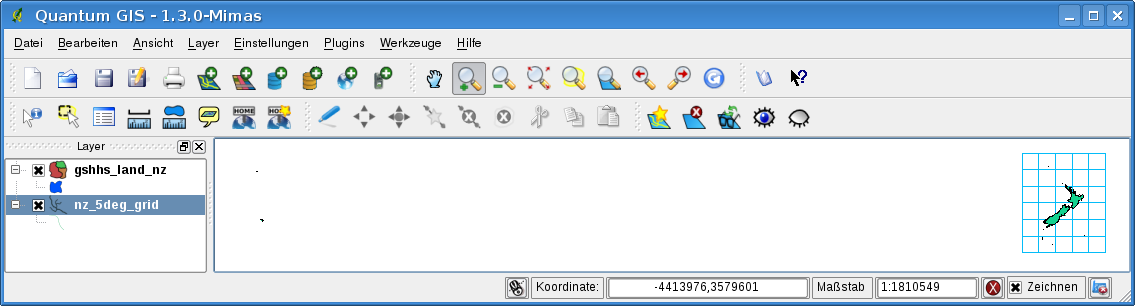
\includegraphics[clip=true, width=\textwidth]{vectorNotWrapping}
\end{center}
\end{figure}

Eine M�glichkeit, dies zu umgehen, bietet PostGIS und die Funktion
\textbf{ST\textunderscore Umschalt\textunderscore
Longitude}.\footnote{\url{http://postgis.refractions.net/documentation/manual-1.4/ST_Umschalt_Longitude.html}}
Die Funktion liest alle Objekte der Karte ein und wenn der L�ngengrad < \degrees{0}
ist, werden \degrees{360} hinzugez�hlt. Das Ergebnis ist eine \degrees{0} -
\degrees{360} Karte, die als Mittelpunkt den L�ngengrad \degrees{180}
verwendet.

\begin{figure}[ht]
   \begin{center}
   \caption{Vektorlayer �ber dem L�ngengrad \degrees{180} nach Anwendung der
PostGIS Funktion \nixcaption}
\label{fig:vector_wrapping}\smallskip
   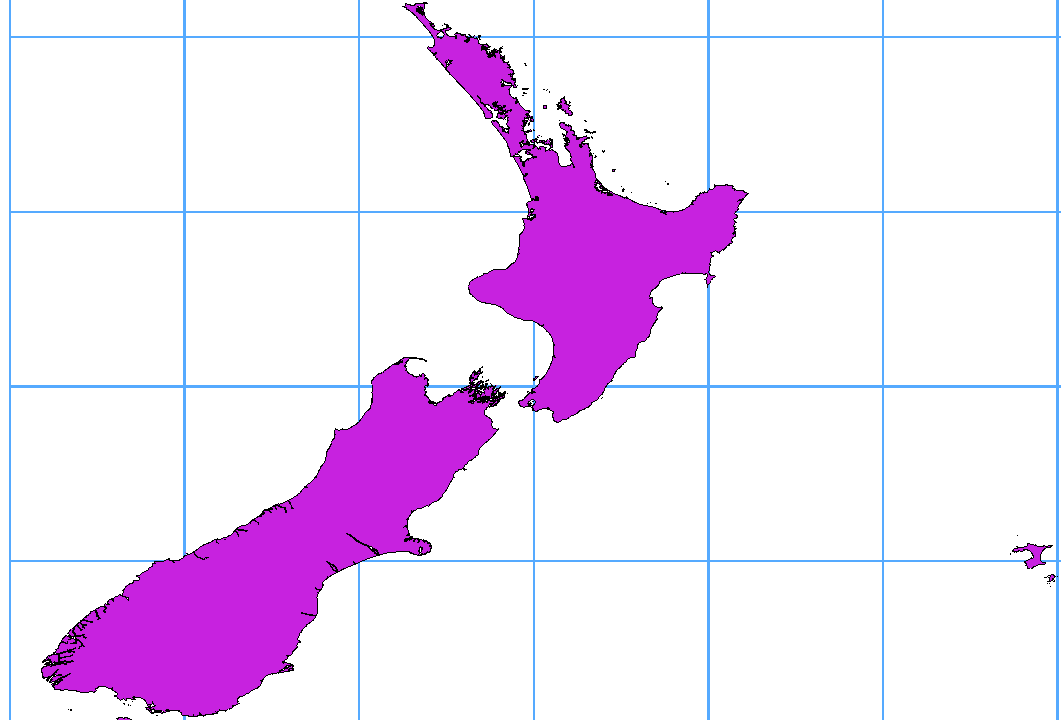
\includegraphics[clip=true, width=9cm]{vectorWrapping}
\end{center}
\end{figure}

\minisec{Beispielanwendung}

\begin{itemize}[label=--]
\item Importiere den Layer nach PostGIS (\ref{sec:loading_postgis_data}) z.B.
mit dem 'PostGIS Manager' oder dem 'SPIT' Plugin.
\item �ffnen Sie das PostGIS Kommandozeilenfenster und geben Sie folgendes
Kommando ein. In diesem Beispiel steht der Name 'TABELLE' f�r den
tats�chlichen Namen der PostGIS Tabelle.\\ 
\texttt{gis\_data=\# update TABELLE set the\_geom=ST\_Umschalt\_longitude(the\_geom);} 
\item Wenn alles geklappt hat, sehen Sie eine Best�tigung mit den Objekten,
die ver�ndert wurden. Danach k�nnen Sie den PostGIS Layer in QGIS als eine
zusammenh�ngende Karte laden (siehe Abbildung \ref{fig:vector_wrapping}).
\end{itemize}

\section{SpatiaLite Layer laden}
\index{SpatiaLite!Layereigenschaften}
\index{Vektorlayer!SpatiaLite}
\index{SpatiaLite!Layer}
\label{label_spatialite}


\includegraphics[width=0.7cm]{mActionAddSpatiaLiteLayer}
Wenn Sie das erste Mal einen Layer aus einer Spatialite Datenbank laden
m�chten, klicken Sie auf das Icon
\toolbtntwo{mActionAddSpatiaLiteLayer}{SpatiaLite Layer hinzuf�gen} in der
Werkzeugleiste oder indem Sie
\dropmenuopttwo{mActionAddSpatiaLiteLayer}{SpatiaLite Layer hinzuf�gen\ldots}
im Men� \mainmenuopt{Layer} ausw�hlen oder indem Sie die Taste \keystroke{L}
dr�cken.
Dies �ffnet einen Dialog, �ber den Sie entweder eine Verbindung zu einer
bereits in QGIS definierten SpatiaLite Datenbank ausw�hlen oder eine
neue Verbindung erstellen k�nnen. Um eine neue Verbindung zu erstellen,
klicken Sie auf den Knopf \button{Neu} und verwenden dann den Dateibrowser,
um eine entsprechende SpatiaLite Datenbank auszuw�hlen. Dabei handelt es sich
um eine Datei mit der Endung \filename{.sqlite}.

Wenn Sie einen Vektorlayer im SpatiaLite Format abspeichern wollen, w�hlen Sie 
den Layer in der Legende aus, benutzen Sie das Kontextmen� der rechten Maustaste 
und klicken Sie auf \dropmenuopt{Speichern als}. Geben Sie den Namen der Ausgabe an, 
w�hlen Sie sqlite als Format aus und das KBS. Danach f�gen Sie noch 'SPATIALITE=YES' 
in das Fenster 'Datenquelle'. Damit sagen Sie OGR, dass eine SpatiaLite Datenbank 
erstellt werden soll. Siehe \url{http://www.gdal.org/ogr/drv_sqlite.html}

\minisec{Einen neuen SpatiaLite Layer erzeugen}

Wenn Sie einen neuen SpatiaLite Layer erzeugen wollen, finden Sie in Kapitel 
\ref{sec:create spatialite} eine Anleitung.

\begin{Tip}\caption{\textsc{SpatiaLite Datenmanagement Plugin}}\index{SpatiaLite! Datenmanagement}. F�r das Managen von SpatiaLite Daten k�nnen Sie das 'Qspatialite' 
Plugin aus dem 'QGIS Contributed Repository' nehmen. Sie k�nnen es mit dem Python 
Plugin Installer installieren. Es bietet QGIS Integration (Import von QGIS Layern, 
Ansicht und Abfrage r�umlicher Tabellen), einen SQL-Editor mit Syntax-Highlighting 
und Auto-Vervollst�ndigung, einen SQL Query Builder f�r Komplexe Abfragen und 
weitere Funktionalit�ten.
\end{Tip}

\section{Vektorlayereigenschaften}\label{sec:vectorprops}
\index{Vektorlayer!Layereigenschaften}

\begin{figure}[H]
   \begin{center}
   \caption{Dialog zur Einstellung von Vektorlayereigenschaften
\nixcaption}\label{fig:vector_symbology}\smallskip
   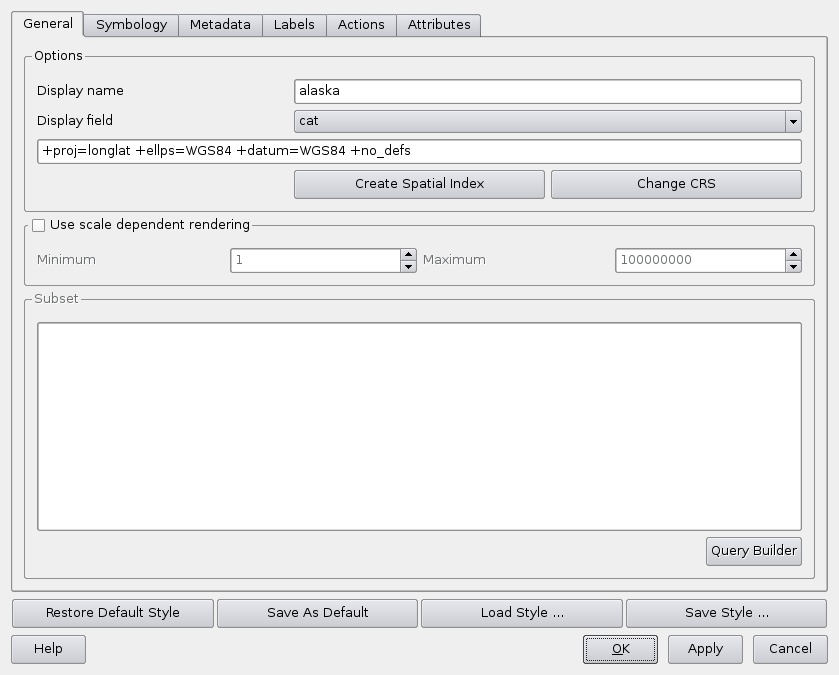
\includegraphics[clip=true, width=16cm]{vectorLayerSymbology}
\end{center}
\end{figure}

Der Dialog \dialog{Layereigenschaften} stellt Einstellungsm�glicheiten und
Informationen zu einem Vektorlayer, seiner Darstellung, Metadaten,
Beschriftungsoptionen, Aktionen und Attributen bereit. Wenn ein Vektorlayer
aus einer PostgreSQL/PostGIS Datenbank geladen wurde, k�nnen �ber den Dialog
\dialog{Layereigenschaften} auch SQL-Abfragen mit dem \dialog{Query Builder}
im Reiter \tab{Allgemein} angewendet werden, indem Sie auf den Knopf
\button{Abfrageerstellung} klicken. Ansonsten m�ssen Sie f�r
OGR-unterst�tzte Formate den \dialog{Query Builder} Dialog �ber den Knopf
\button{Erweiterte Suche} im Attributtabellen Fenster starten
(vgl. Kapitel~\ref{sec:query_builder}). Um den Dialog f�r die
Layereigenschaften zu �ffnen, doppelklicken Sie auf den Namen des Layers in
der Legende oder w�hlen mit der rechten Maustaste \dialog{Eigenschaften} aus.

\subsection{Stil}\label{sec:symbology}
\index{Vektorlayer!Stil}

Ab der \qg Version 1.4 wurde parallel eine neue Darstellung integriert, um 
die alte zu verbessern und letztlich auch abzul�sen. \qg 1.7 benutzt die 
neue Darstellung jetzt als Default-Einstellung. Ihnen stehen dadurch eine 
Vielzahl von Verbesserungen und neuen Funktionalit�ten zur Verf�gung.

Eine Beschreibung der alten Darstellung finden Sie in Abschnitt 
\ref{sec:oldsymbology}.

\subsection{Neue Darstellung - Symbology-NG}

In QGIS \CURRENT ist parallel zur oben beschriebenen Darstellung eine 
neue Darstellung integriert worden. Diese bietet eine Vielzahl von 
Verbesserungen und neuer Funktionalit�ten und wird in einer der zuk�nftigen 
QGIS Versionen die aktuelle Standarddarstellung abl�sen.

Um derzeit in die neue Darstellung zu wechseln, ist es notwendig, auf den 
Knopf \button{Neue Darstellung} im Reiter \tab{Stil} des 
\dialog{Layereigenschaften} Dialogs zu dr�cken. Sie k�nnen die neue 
Darstellung auch als Standard setzen im Reiter \tab{Stil} 
des Men�s \mainmenuopt{Einstellungen} \arrow \dropmenuopt{Optionen}. Aktivieren Sie 
dazu das Kontrollk�stchen \checkbox{Darstellung der n�chsten Generation 
verwenden}.

\minisec{Die neue Darstellung verstehen}

Es gibt drei verschiedene Symboltypen: Zeichensymbole (f�r Punkte), 
Liniensymbole (f�r Linien) und F�ll- und Randsymbole (f�r Polygone). 
Symbole k�nnen aus einer oder mehreren Symbolebenen bestehen. Sie k�nnen 
die Farbe eines Symbols festlegen, und diese gilt dann f�r alle weiteren 
Symbolebenen. Bei einigen Symbolen kann die Symbolfarbe gesperrt sein, 
bei diesen kann die Farbe dann nicht ge�ndert werden. Dies ist n�tzlich, 
wenn man die Farbe eines Multilayer-Symbols definiert.

\minisec{Vorhandene Typen von Symbolebenen}
\label{symboltypes}

\begin{itemize}[label=--]
\item Punktlayer
\begin{itemize}[label=--]
\item \textbf{Schriftmarkierung}: Darstellung mit einer definierten Schrift.
\item \textbf{Einfache Markierung}: Darstellung mit einem definierten Symbol.
\item \textbf{SVG Markierung}: Darstellen mit einem SVG-Bild.
\end{itemize}
\item Linienlayer
\begin{itemize}[label=--]
\item \textbf{Liniendekoration}: Hinzuf�gen einer Liniendekoration, z.B. Pfeil, um die Richtung der Linie darzustellen.
\item \textbf{Markierungslinie}: Darstellen einer Linie durch wiederholung eines Symbols.
\item \textbf{Einfache Linie}: Darstellen einer Linie (mit festgelegter Breite, Farbe und Stiftstil).
\end{itemize}
\item Linienlayer
\begin{itemize}[label=--]
\item \textbf{Zentrierte F�llung}: Darstellung eines Zentroids mit einem definierten Symbol.
\item \textbf{SVG-F�llung}: F�llen einer Fl�che mit einem SVG-Bild. 
\item \textbf{Einfache F�llung}: F�llen einer Fl�che (mit festgelegter Farbe, F�ll- und Randstil). 
\item \textbf{Rand: Liniendekoration}: Darstellen einer Randlinie durch Hinzuf�gen einer Liniendekoration.
\item \textbf{Rand: Markierungslinie}: Darstellen einer Randlinie durch wiederholung eines Symbols.
\item \textbf{Rand: Einfache Linie}: Darstellen einer Randlinie (mit festgelegter Breite, Farbe und Stiftstil).
\end{itemize}
\end{itemize}

\minisec{Farbverl�ufe}

Farbverl�ufe werden verwendet, um eine Spannweite von Farben zu definieren, die 
f�r die Darstellung verwendet werden sollen. Die Symbolfarbe wird entsprechend des 
definierten Farbverlaufs angewendet. Es gibt drei Typen: 

\begin{itemize}[label=--]
\item \textbf{Gradient}: Linearer Gradient von einer zu anderen Farben.
\item \textbf{Random}: Zuf�llig erstellte Farben aus einem festgelegten Farbraum.
\item \textbf{Farbbrauer}: Erstellen von Farbbereichen aus einem Farbschema und 
einer definierten Anzahl von Farbklassen.
\end{itemize}

Sie k�nnen neue Farbverl�ufe im Reiter \tab{Farbverlauf} des Stilmanagers definieren 
(siehe Kapitel \ref{subsec:stylemanager}), indem Sie auf \button{Hinzuf�gen} klicken 
und dann einen Farbverlauftyp ausw�hlen. 

\minisec{Stile}

Ein Stil gruppiert eine Reihe unterschiedlicher Symbole und Farbanstiege. 
Dadurch ist es m�glich, eigene, bevorzugte oder h�ufig benutzte Symbole 
festzulegen und abzuspeichern. Stile (Symbole und Farbanstiege) haben 
immer einen Namen, �ber den Sie gesucht werden k�nnen. Es gibt mindestens 
einen ver�nderbaren Standard-Stil in QGIS und Sie k�nnen weitere Stile hinzuf�gen. 

\minisec{Darstellungen}

�ber die Darstellung wird festgelegt, wie Objekte als Symbole angezeigt werden. 
Es gibt vier Arten der Darstellung: Einzelsymbol, Kategorisiert (in der alten 
Darstellung auch Eindeutiger Wert genannt), Abgestuft und Regelbasierend. Die Vorgabe 
Fortlaufende Farbe gibt es nicht, da es sich dabei um einen Spezialfall der 
kategorisierten Darstellung handelt. Die kategorisierte und abgestufte Darstellung 
wird erreicht, indem ein Symbol mit einem Farbanstieg definiert wird - die 
Farben der Symbole werden dann passend gesetzt. 

\subsection{Mit der neuen Darstellung arbeiten}

Der Dialog erm�glicht es, aus den vier Darstellungsarten auszuw�hlen: Einzelsymbol, Kategorisiert, Abgestuft und Regelbasierend. In 
Abh�ngigkeit von der ausgew�hlten Darstellungart bietet der Reiter 
\tab{Stil} unterschiedliche Optionen und Einstellungsm�glichkeiten, die 
im folgenden Abschnitt beschrieben werden. �ber die neue Darstellung k�nnen Sie 
auch den \button{Stilmanager} �ffnen (siehe Kapitel \ref{subsec:stylemanager}). 
Der Stilmanager erm�glicht es, neue Symbole zu erstellen und vorhandene zu editieren 
oder zu l�schen. 

\minisec{Einzelsymbol Darstellung}

Die Einzelsymbol Darstellung wird verwendet, um alle Objekte eines Vektorlayers 
mit einem, definierten Symbol darzustellen. Die Eigenschaften, die dabei im Reiter
\tab{Stil} festgelegt werden k�nnen, h�ngen teilweise vom Layertyp ab, 
aber alle Layertypen (Punkt, Linie und Polygon) nutzen folgende Strukturen. In der 
oberen linken Ecke des Reiters wird ein Preview des Symbols angezeigt, das dann 
auch dargestellt wird. 

Im unteren Bereich des Reiters, wird eine Liste bereits vorhandener Symbole 
angezeigt, die direkt ausgew�hlt werden k�nnen. Das aktuelle 
Symbol kann bearbeitet werden, in dem man auf den Knopf \button{�ndern} 
dr�ckt, woraufhin sich der Dialog \dialog{Symboleigenschaften} �ffnet. Oder Sie 
dr�cken auf den Knopf \button{�ndern} mit dem aktuellen Farbsymbol und k�nnen 
dann in einem Standard-Farbdialog eine neue Farbe definieren. 

Nachdem Sie alle notwendigen Anpassungen gemacht wurden, k�nnen Sie das neue 
Symbol mit den Knopf \button{Als Stil speichern} zu der Liste bereits 
vorhandener Symbole hinzuf�gen.  

\begin{figure}[h]
\centering
\caption{Optionen f�r die Darstellung von Einzelsymbolen \nixcaption}
   \subfloat[Eigenschaften von Punkt-Einzelsymbolen] {\label{subfig:singleNG1}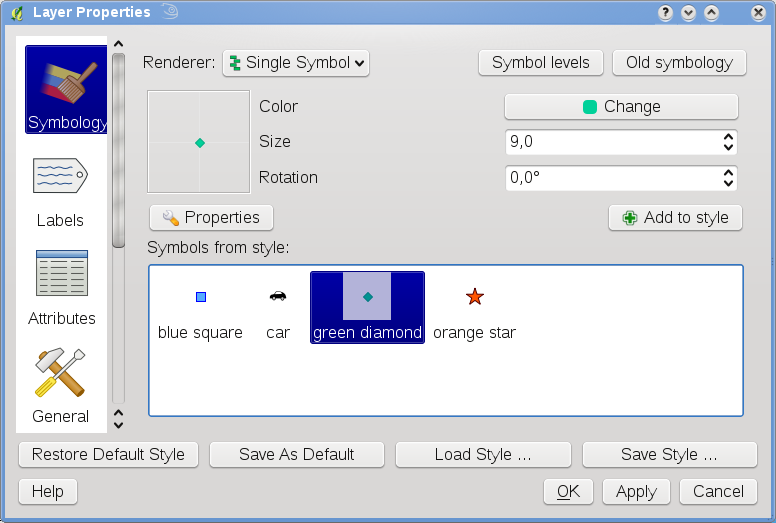
\includegraphics[clip=true, width=0.3\textwidth]{singlesymbol_ng_point}}\hspace{0.33cm}
   \subfloat[Eigenschaften von Linien-Einzelsymbolen] {\label{subfig:singleNG2}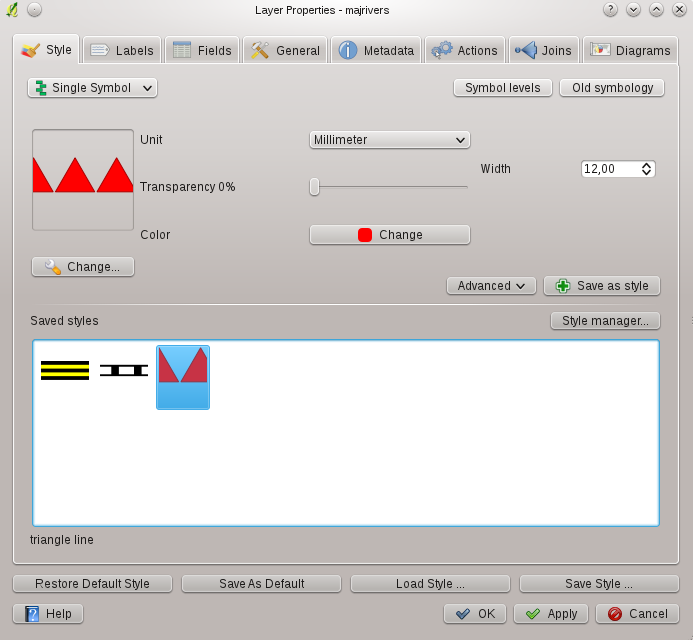
\includegraphics[clip=true, width=0.3\textwidth]{singlesymbol_ng_line}}\hspace{0.33cm}
   \subfloat[Eigenschaften von Polygon-Einzelsymbolen] {\label{subfig:singleNG3}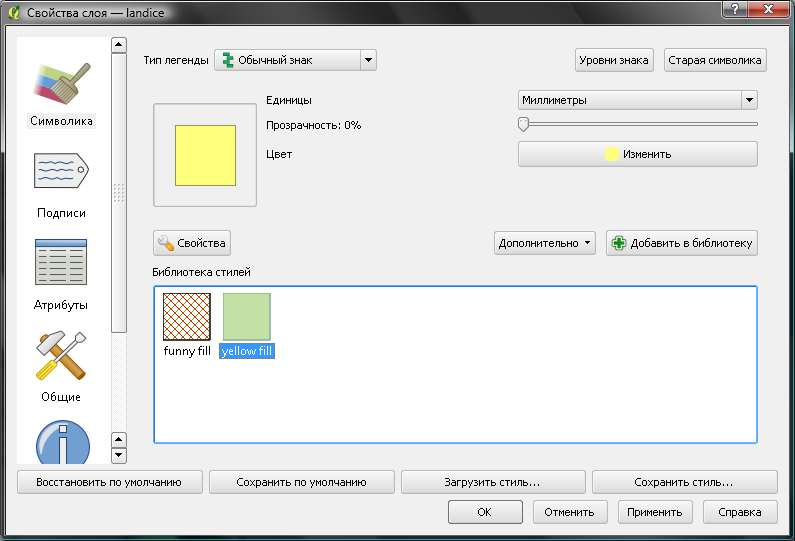
\includegraphics[clip=true, width=0.3\textwidth]{singlesymbol_ng_area}}
\end{figure}

\minisec{Kategorisierte Darstellung}

Die kategorisierte Darstellung wird verwendet, um alle Objekte eines Vektorlayers
mit einem, definierten Symbol darzustellen. Dabei reflektiert der Farbwert des 
Symbols den Wert eines Objektattributs. Im Reiter \tab{Stil} kann 
ausgew�hlt werden:

\begin{itemize}[label=--]
\item Das Attribut (�ber die Auswahl Spalte)
\item Das Symbol (�ber die Auswahl Symbol)
\item Die Farbe (�ber die Auswahl Farbanstieg)
\end{itemize}

Der Knopf \button{Erweitert} in der unteren rechten Ecke des Dialogs erm�glicht 
die Auswahl von Attributspalten f�r die Drehung und Gr��enskalierung.
Zur Veranschaulichung wird im unteren Teil des Reiters eine Liste mit allen 
Attributen und der jeweils verwendeten Symbolfarbe angezeigt. Das Beispiel in 
Abbildung \ref{fig:catsymNG} zeigt den Dialog Kategorisierte Darstellung f�r 
den Vektorlayer \filename{rivers} des QGIS-Beispieldatensatzes. 

\begin{figure}[ht]
   \begin{center}
   \caption{Optionen f�r die Darstellung von kategorisierter Symbole \nixcaption}\label{fig:catsymNG}\smallskip
   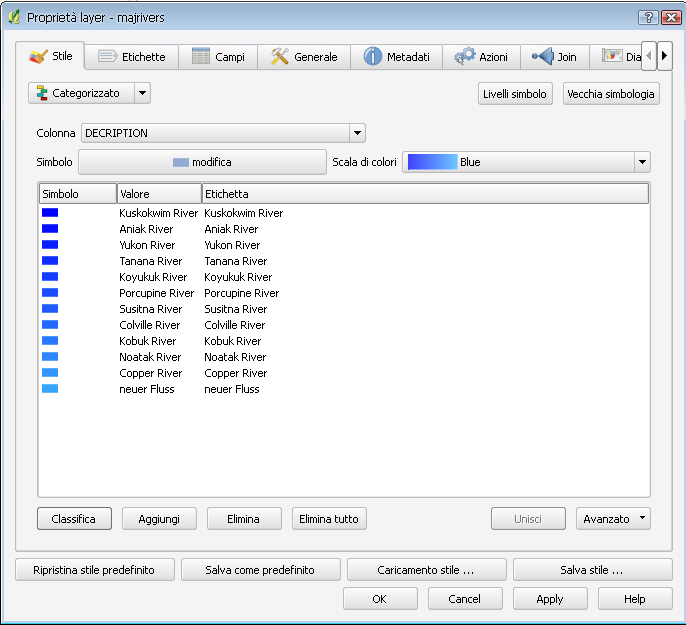
\includegraphics[clip=true, width=10cm]{categorysymbol_ng_line}
\end{center}
\end{figure}

Sie k�nnen einen individuellen Farbverlauf erstellen, indem Sie im Bereich 
Farbverlauf \dialog{Neuer Farbverlauf} ausw�hlen. Dadurch �ffnet sich ein 
neuer Dialog und Sie k�nnen ausw�hlen zwischen Gradient, Zuf�llig und Farbbrauer. 
Jede dieser Optionen erm�glicht dann, die Farbschritte festzulegen. Ein Beispiel 
finden Sie in Abbildung \ref{fig:ccrg}.


\begin{figure}[ht]
   \centering
   \caption{Beispiel eines individuellen Farbverlaufs mit mehreren Farbstufen \nixcaption}\label{fig:ccrg}
   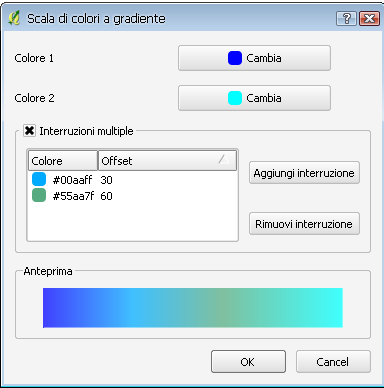
\includegraphics[clip=true, width=10cm]{customColorRampGradient}
\end{figure}

\minisec{Abgestufte Darstellung}

Die abgestufte Darstellung wird verwendet, um alle Objekte eines Vektorlayers
mit einem, definierten Symbol darzustellen, Dabei reflektiert der Farbwert die 
Klassifikation von Objektattributen innerhalb definierter Klassen.

Analog zur kategorisierten Darstellung erm�glicht der Reiter \tab{Stil} 
folgende Einstellungen:

\begin{itemize}[label=--]
\item Das Attribut (�ber die Auswahl Spalte)
\item Das Symbol (�ber die Auswahl Symbol)
\item Die Farbe (�ber die Auswahl Farbanstieg)
\end{itemize}

Zus�tzlich k�nnen Sie die Anzahl der Klassen und den Modus f�r die Klassifizierung 
festlegen. Im unteren Teil des Reiters wird eine Liste der Klassen, mit deren 
Darstellung, der Range und dem Label angezeigt. Die vohandenen Modi sind:
The available modes are:

\begin{itemize}
 \item Gleiches Intervall
 \item Quantile
 \item Nat�rliche Unterbrechungen (Jenks)
 \item Standardabweichung
 \item Sch�ne Unterbrechungen
\end{itemize}

Das Listenfeld im unteren Bereich des Reiters \tab{Stil} zeigt die 
festgelegten Werteklassen und -bereiche, Beschriftungen und Symbole, die dargestellt 
werden.

Das Beispiel in Abbildung \ref{fig:gradsymNG} zeigt den Dialog 
\dialog{Abgestufte Darstellung} f�r den Vektorlayer rivers des 
QGIS-Beispieldatensatzes.

\begin{figure}[ht]
   \begin{center}
   \caption{Optionen f�r die Darstellung abgestufter Symbole \nixcaption}\label{fig:gradsymNG}\smallskip
   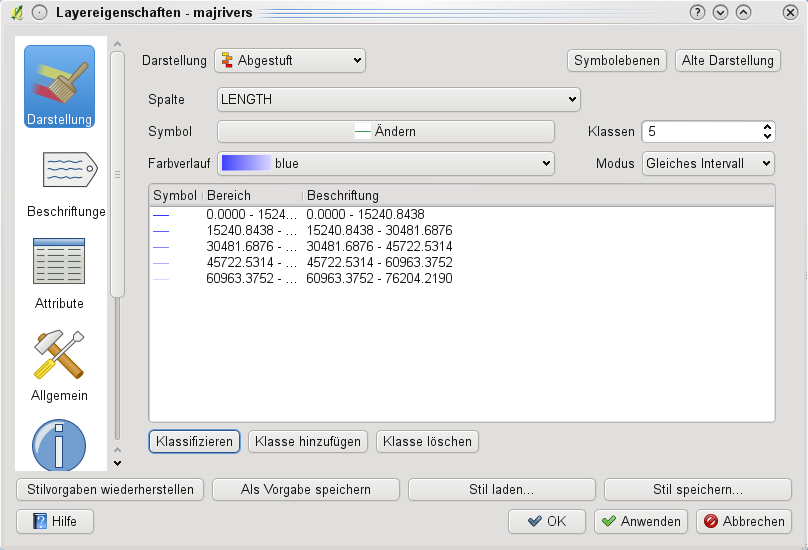
\includegraphics[clip=true, width=10cm]{graduatesymbol_ng_line}
\end{center}
\end{figure}

\minisec{Regelbasierende Darstellung}

Die regelbasierende Darstellung wird verwendet, um die Objekte eines Layers nach 
selbst festgelegten Regeln darstellen zu k�nnen, die dann die Zugeh�rigkeit zu 
einer bestimmten Klasse zeigt. Die Regeln basieren auf SQL-Abfragen. Sie k�nnen 
dazu auch den Abfrageeditor verwenden. Der Dialog erlaubt auch das gruppieren 
von Regeln durch Filter und Massstabsangaben. Ausserdem gibt es noch die M�glichkeit, 
die Kontrollk�stchen \checkbox{Symbolebenen aktivieren} und \checkbox{Nur erste 
passende Regel verwenden} auszuw�hlen. 

Das Beispiel in Abbildung~\ref{fig:rulesymNG} zeigt den Dialog der regelbasierenden 
Darstellung f�r den Layer 'rivers' des QGIS Beispieldatensatzes.

\begin{figure}[ht]
   \centering
   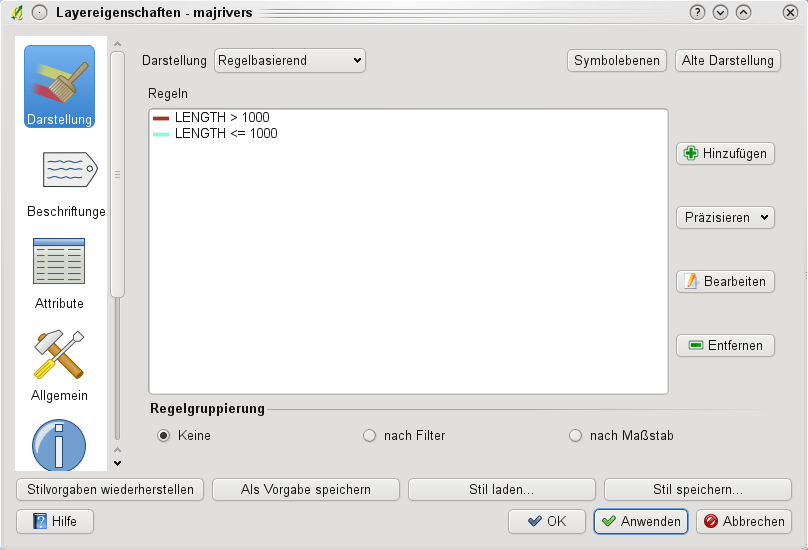
\includegraphics[clip=true, width=10cm]{rulesymbol_ng_line}
   \caption{Dialog f�r regelbasierende Darstellung \nixcaption}\label{fig:rulesymNG}
\end{figure}

\minisec{Punkt-Verschiebung}
\label{new_generation_sym}
\index{Vektorlayer!Punkt-Verschiebung}
\index{Punkt-Verschiebung}

F�r Punktlayer gibt es eine Darstellungsart, mit der es m�glich ist, s�mtliche 
Punkte eines Layers auch dann darzustellen, wenn sie sich teilweise an derselben Stelle 
befinden. Dies kann zum Beispiel bei Zeitrihen der Fall sein. Die Punkte werden dabei 
um ein Zentrumssymbol herum auf einem Versatzkreis angeordnet und dargestellt, 
siehe Abbildung~\ref{fig:poidissymNG}. Die Punkt-Verschiebung steht nur zur Verf�gung, 
wenn Sie das Kern-Plugin Verschiebungserweiterung geladen haben.

\begin{figure}[ht]
   \centering
   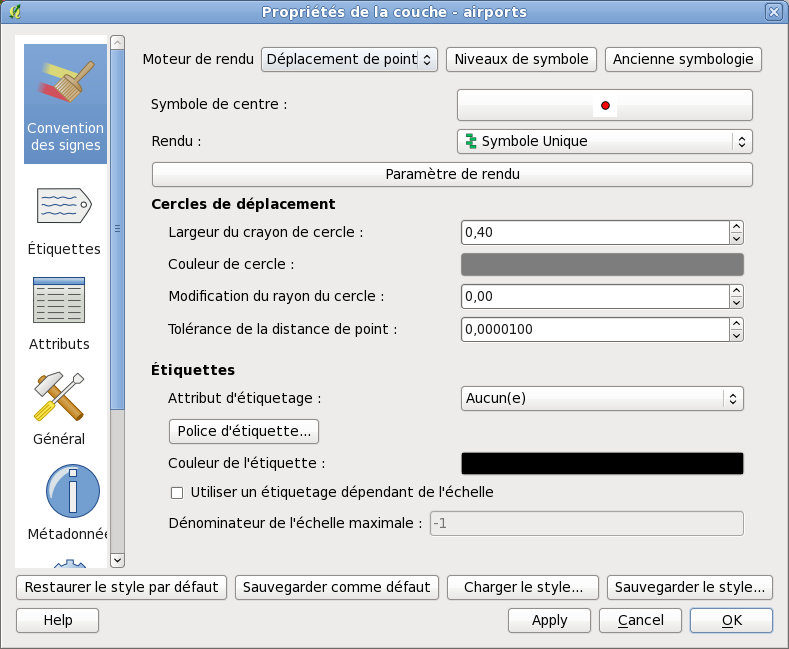
\includegraphics[clip=true, width=10cm]{poi_displacement}
   \caption{Dialog f�r Punkt-Verschiebung \nixcaption}\label{fig:poidissymNG}
\end{figure}

\minisec{Symboleigenschaften}

Der Dialog \dialog{Symboleigenschaften} erlaubt es, ein Symbol zu definieren. Im 
oberen linken Bereich befindet sich immer ein Preview des aktuellen Symbols. 
Darunter sind die Symbollayer aufgelistet, aus denen sich das Symbol zusammensetzt. 
Um den Dialog \dialog{Symboleigenschaften} zu �ffnen, dr�cken Sie den Knopf 
\dropmenuopttwo{mActionOptions}{Eigenschaften} im Reiter \tab{Symbology} des 
Dialogs \dialog{Layereigenschaften}.

Mit den Kontrollkn�pfen k�nnen Symbollayer hinzugef�gt oder entfernt werden, ihre 
Reihenfolge ver�ndert oder die Layerfarbe gesperrt werden. Im rechten Teil des 
Dialogs werden die Symbollayereigenschaften dargestellt. Am wichtigsten ist hier 
die Symbollayertyp Auswahl. Die Optionen sind abh�ngig vom Layertyp (Punkt, Linie 
Polygon). Eine Liste der vorhandenen Symbollayertypen finden Sie in Kapitel 
\ref{symboltypes}.


\begin{figure}[h]
\centering
\caption{Symboleigenschaften festlegen \nixcaption}
   \subfloat[Linie aus drei einfachen Linien] {\label{subfig:symprops1}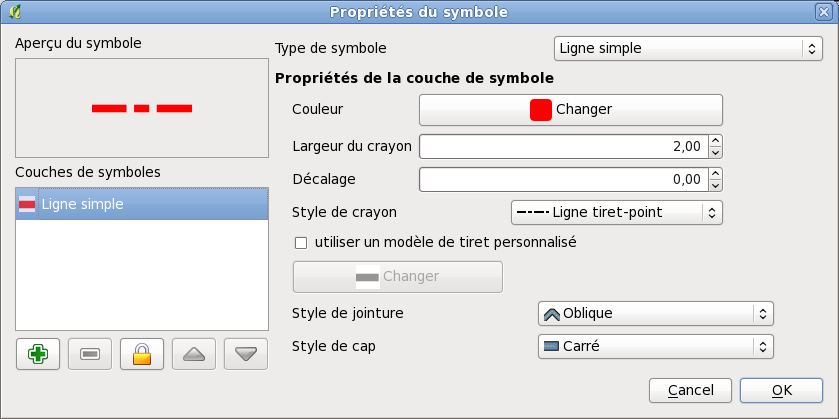
\includegraphics[clip=true, width=0.3\textwidth]{symbolproperties1}}\hspace{0.33cm}
   \subfloat[Symboleigenschaften f�r Punkte] {\label{subfig:symprops2}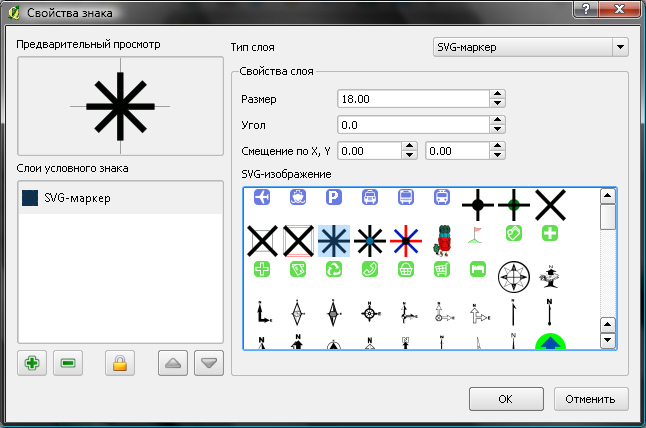
\includegraphics[clip=true, width=0.3\textwidth]{symbolproperties2}}\hspace{0.33cm}
   \subfloat[F�llstil f�r Polygone] {\label{subfig:symprops3}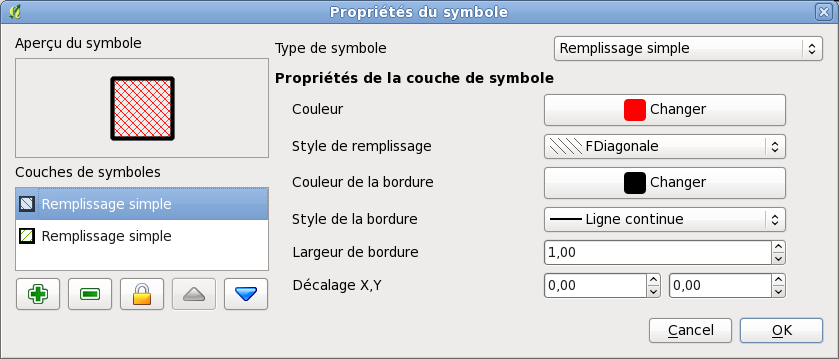
\includegraphics[clip=true, width=0.3\textwidth]{symbolproperties3}}
\end{figure}

\subsection{Stilmanager zum managen von Symbolen und Farbanstiegen}\label{subsec:stylemanager}

Der Stilmanager ist eine kleine Applikation, in der alle vohandenen Symbole 
und Farbanstiege aufgelistet werden. Es erm�glicht au�erdem, Symbole hinzuzuf�gen 
und/oder zu entfernen. Starten Sie den Stilmanager, indem Sie auf 
\mainmenuopt{Einstellungen} \arrow \dropmenuopt{Stilmanager} im Hauptmen� klicken.

\begin{figure}[ht]
   \begin{center}
   \caption{Stilmanager zum managen von Symbolen und Farbanstiegen \nixcaption}\label{fig:stylemanager}\smallskip
   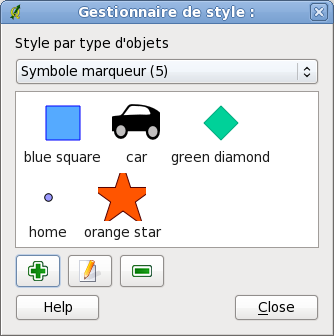
\includegraphics[clip=true, width=7cm]{stylemanager}
\end{center}
\end{figure}

\subsection{Alte Darstellung}\label{sec:oldsymbology}
\index{Vektorlayer!Alte Darstellung}

\textbf{Bemwerkung}: \qg 1.7 unterst�tzt weiterhin die Verwendung der alten 
Darstellung, auch wenn wir empfehlen, mit der neuen Darstellung zu arbeiten, 
siehe Kapitel \ref{sec:symbology}, da die alte Darstellung in einer der 
kommenden Versionen verschwinden wird.

Wenn Sie die alte Darstellung verwenden wollen, klicken Sie auf den Knopf 
\button{Alte Darstellung} im \tab{Stil} Reiter der \dialog{Layereigenschaften}.

Sie k�nnen auch einstellen, dass die alte Darstellung wieder der Standard ist, 
in dem Sie das Kontrollk�stchen \checkbox{Darstellung der n�chsten Generation verwenden} 
im Reiter \tab{Stil} im Men� \mainmenuopt{Einstellungen} \arrow 
\dropmenuopt{Optionen} deaktivieren. 

Die alte QGIS Darstellung unterst�tzt folgende Darstellungsarten:

\begin{description}
\item[Einfaches Symbol] - eine definierte Darstellung wird allen Objekten des
Layers zugewiesen.\index{Vektorlayer!Darstellung!Einfaches Symbol}
\item[Abgestuftes Symbol] - Objekten eines Layers wird in Abh�ngigkeit von
einer Attributspalte und einer definierten Anzahl von Klassen eine
Darstellung zugewiesen.\index{Vektorlayer!Darstellung!Abgestuftes Symbol}
\item[Fortlaufende Farbe] - Objekten eines Layers wird anhand von definierten,
numerischen Werten eine fortlaufende Farbe
zugewiesen.\index{Vektorlayer!Darstellung!Fortlaufende Farbe}
\item[Eindeutiger Wert] - eine definierte Darstellung wird jeder Objektklasse
eines Layers anhand einer definierten Attributspalte
zugewiesen.\index{Vektorlayer!Darstellung!Eindeutiger Wert}
\end{description}

Um die Darstellung f�r einen Layer zu �ndern, klicken Sie einfach doppelt auf 
den seinen Legendeneintrag, so dass der Dialog \dialog{Layereigenschaften} 
angezeigt wird. \index{Vektorlayer!Darstellung!Ver�ndern}

\begin{figure}[ht]
\centering
\caption{Darstellungsoptionen \nixcaption}
   \subfloat[Einfaches Symbol]{
   \label{subfig:single_symbol}
   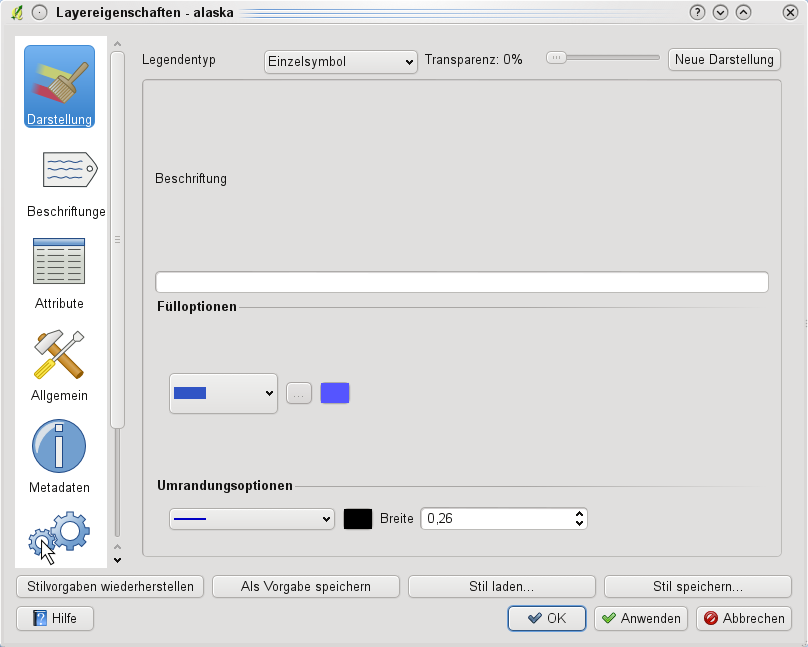
\includegraphics[clip=true, width=0.4\textwidth]{vectorClassifySingle}}
   \hspace{1cm}
   \subfloat[Abgestuftes Symbol]
   {\label{subfig:graduated_symbol}
   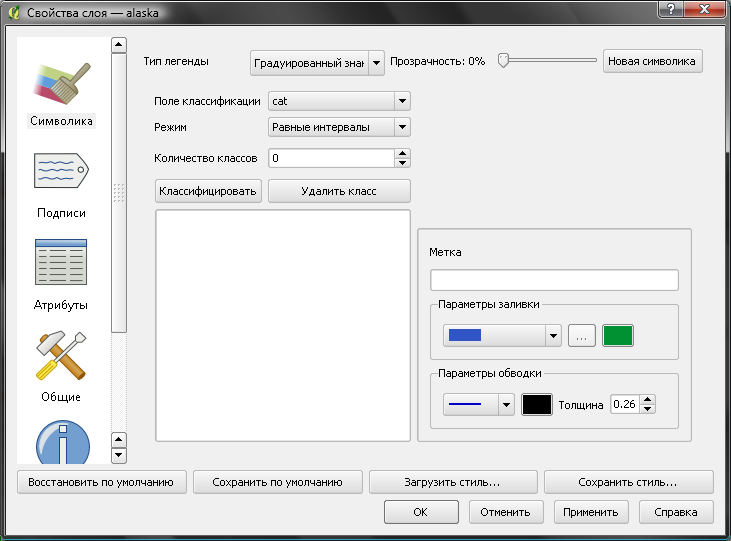
\includegraphics[clip=true, width=0.4\textwidth]{vectorClassifyGraduated}}
   \hspace{1cm}
   \subfloat[Fortlaufende Farbe]{
   \label{subfig:cont_color}
   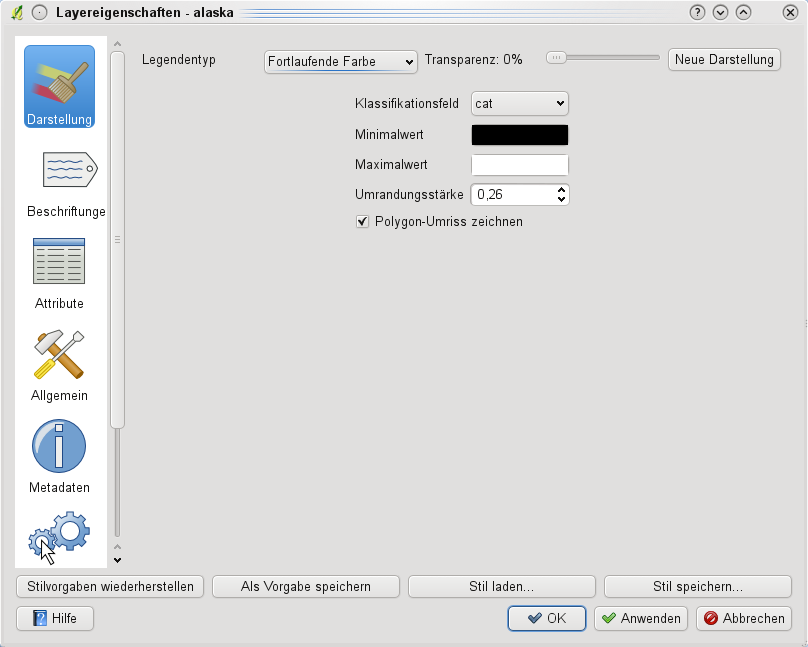
\includegraphics[clip=true, width=0.4\textwidth]{vectorClassifyContinous}}
   \hspace{1cm}
   \subfloat[Eindeutiger Wert]{
   \label{subfig:unique_val}
   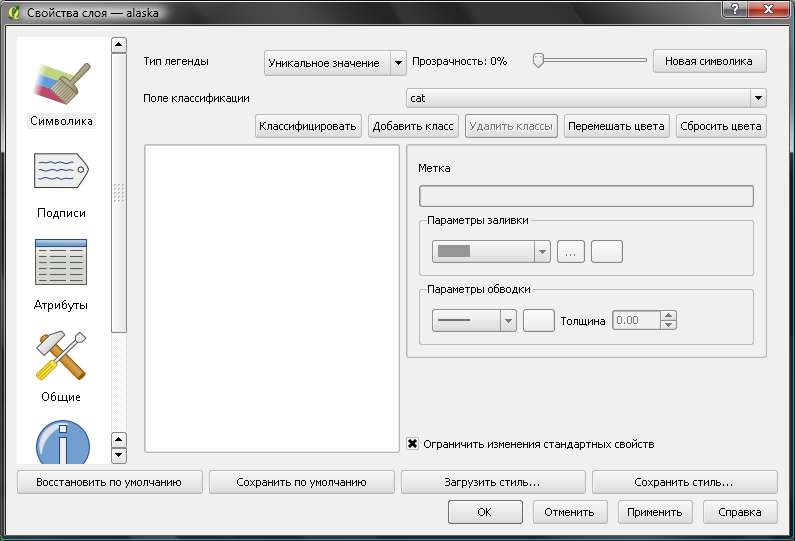
\includegraphics[clip=true, width=0.4\textwidth]{vectorClassifyUnique}}
\end{figure}

\minisec{Stiloption} \label{sec:style_options}
\index{Vektorlayer!Stiloptionen}

Innerhalb des Reiters \tab{Stil} k�nnen auch Stiloptionen f�r
Vektorlayer definiert werden. Abh�ngig vom ausgew�hlten Legendentyp k�nnen
Vektorobjekte auch klassifiziert dargestellt werden. Die folgenden
Stiloptionen stehen zur Verf�gung: 

\begin{description}
\item [F�lloptionen]
\begin{description}
 \item[F�llstil] - Definition des F�llstils von Polygonen. Neben Ausgef�llt
und Nicht gef�llt stehen zahlreiche Schraffurstile und die M�glichkeit eine
eigene Textur in Form eines Bildes zu laden. W�hlen Sie dazu
\selectstring{F�llstil}{? Texture}, dr�cken Sie auf den Knopf \browsebutton
und w�hlen Sie eine Bilddatei. Aktuell wird als Datenformat \filename{*.jpeg,
*.xpm, und *.png} unterst�tzt.
 \item[F�llfarbe] - Definition der F�llfarbe von Polygonen.
\end{description}
\begin{description}
\item [Umrandungsoptionen]
 \item[Umrandungsfarbe] - Definition der Farbe f�r Linien und Umrandunglinien
von Objekten
 \item[Umrandungsbreite] - Definition der Linienbreite f�r Linien und
Umrandunglinien von Objekten
\end{description}
\end{description}

Nachdem Sie die Darstellung f�r den Layer festgelegt haben, k�nnen Sie die
Definition als Datei mit der Endung \filename{*.qml} speichern. Dazu dr�cken
Sie auf den Knopf \button{Stil speichern \ldots} und entsprechend zum Laden
einer Stildefinition auf den Knopf \button{Stil laden \ldots}.

Wenn Sie m�chten, dass immer eine bestimmte Stildefinition verwendet wird, wenn
Sie einen Layer laden, klicken Sie auf den Knopf \button{Als Standard
speichern}. Wenn Sie die Darstellung des Layers ver�ndern, aber lieber wieder
zur abgespeicherten Standard-Stildefinition zur�ckkehren m�chten, dr�cken Sie
den Knopf \button{Standardstil wiederherstellen}.

\minisec{Vektor Transparenz}\label{sec:vect_transparency}
\index{Vektorlayer!Transparenz}

Innerhalb des Reiters \tab{Stil} kann auch die Transparenz f�r den
Layer festgelegt werden. Dazu verschieben Sie den Regler
\slider{Transparenz} wie in Abbildung~\ref{fig:vector_symbology} zu
sehen. Dies ist sehr n�tzlich, wenn Sie mehrere Vektorebenen miteinander
�berlagern m�chten.

\subsection{Beschriftungen}\index{Beschriftung}

Analog zur Darstellung, stellt \qg \CURRENT derzeit auch zwei Beschriftungen 
zur Verf�gung. Der Reiter \tab{Beschriftungen} enth�lt noch die alte 
Beschriftung. Die neue Beschriftung ist noch als Kern-Erweiterung implementiert, 
und wird die alte Beschriftung in einer der kommenden Versionen ersetzen.

Wir empfehlen die neue Beschriftung zu verwenden. Sie ist in Kapitel 
\ref{newlabel} beschrieben.

Mit der alten Beschriftungen k�nnen Sie Objekte beschriften und die
Anordnung, den Schriftstil, die Ausrichtung, Pufferung und Position der
Beschriftung festlegen. Als Beispiel stellen wir die Beschriftung der 
Karte lakes.shp des QGIS Beispieldatensatzes \filename{qgis\_example\_dataset} 
vor:

\begin{enumerate}
\item Laden der Shapes \filename{alaska.shp} und \filename{lakes.shp}
\item Zoomen Sie ein wenig in ein Gebiet mit ein paar Seen
\item Aktivieren die den \filename{lakes} Layer
\item �ffnen Sie den \dialog{Layereigenschaften} Dialog
\item Klicken Sie auf den \tab{Beschriftungen} Reiter
\item Aktivieren Sie die Checkbox \checkbox{Zeige Beschriftungen an}
\item W�hlen Sie als \selectstring{Beschreibungsfeld}{NAMES} aus der Attributtabelle
\item Geben Sie eine Beschriftungsvorgabe f�r Seen ein, die keine
Beschriftung im \guilabel{NAMES} Feld enthalten.
\item Wenn eine Spalte Attribute enth�lt, die �ber mehrere Zeilen gehen,
aktivieren Sie das Kontrollk�stchen \checkbox{Mehrzeilige Beschriftungen?}.
QGIS wird dann die Zeilenumbr�che entsprechend setzen. Dabei handelt es sich
um das \textbf{einfache} Zeichen \textbackslash n, (nicht zwei einzelne
Zeichen, wie ein Backslash \textbackslash gefolgt von dem Zeichen n). Um 
Zeilenumbr�che in ein Attributfeld einzuf�gen, konfigurieren Sie bitte 
das Bearbeitungselement f�r die Spalte auf Texteditor.
\item Klicken Sie auf \button{Anwenden}.
\end{enumerate}

Nun werden Beschriftungen angezeigt, aber sie sind wahrscheinlich noch zu
gro"s und schlecht plaziert bezogen auf die Objekte des Layers
\filename{lakes}. Klicken Sie auf den Knopf \button{Schrift}, �ndern Sie
Schriftart, -stil und -gr��e und dr�cken dann auf \button{OK}. �ndern Sie
entsprechend auf die \button{Farbe} der Beschriftung.

Um die Position der Beschriftungen zu �ndern f�hren Sie folgende Schritte
durch:

\begin{enumerate}
\item W�hlen Sie einen der Kn�pfe im Platzierungsfeld. In diesem Beispiel
klicken auf den Knopf \radiobuttonon{Rechts}.
\item Klicken Sie auf den Knopf \button{Anwenden}, um die Ver�nderungen
zu sehen und schlie�en Sie dann den Dialog.
\end{enumerate}

Nun sehen die Beschriftungen schon besser aus, aber Sie liegen noch ein wenig
zu nah an den Objekten. Dies k�nnen Sie �ndern, indem Sie auf Position
klicken und einen X- und Y-Offset einstellen. Mit einem X-Offset mit
dem Wert 5 sind die Beschriftungen wahrscheinlich schon besser lesbar.
Ansonsten passen Sie die Werte entsprechend an.

Die letzte Anpassung der Beschriftung ist das Puffern. Dies bedeutet, dass
die Beschriftung mit einem farblichen Puffer hinterlegt werdem, damit man sie
besser lesen kann. Um die Beschriftungen der Karte \filename{lakes.shp} zu
Puffern sind folgende Schritte notwendig:

\begin{enumerate}
\item Aktivieren Sie das Kontrollk�stchen \checkbox{Beschriftungen freistellen}.
\item W�hlen Sie eine Gr��e und eine Farbe
\item Klicken Sie auf \button{Anwenden}, um das Ergebnis zu betrachten.
\end{enumerate}

Wenn Sie mit dem Resultat noch nicht gl�cklich sind, ver�ndern Sie die
Einstellungen weiter, bis es Ihnen gef�llt und klicken Sie jeweils immer auf
den Knopf \button{Anwenden}, um es anzuschauen. Ein Puffer der Gr��e 2 gibt
normalerweise recht ansehnliche Ergebnisse. Sie k�nnen die Puffergr��e
�brigens auch in Karteneinheiten definieren, wenn Ihnen das besser gef�llt.

Als weitere Einstellungen im Reiter \tab{Beschriftungen} ist es m�glich, das
Erscheinungsbild der Beschriftungen anhand von Angaben aus der
Attributtabelle des Layers zu �ndern. �ber die Bereiche Datendefinierter
Stil, Datendefinierter Puffer und Datendefinierte Position k�nnen Sie alle
notwendigen Parameter anhand von Inhalten aus Attributspalten definieren.

Beachten Sie, dass es im unteren Bereich auch ein kleines
\classname{Vorschau}-Feld gibt, in dem alle �nderungen angezeigt werden.

\subsection{Neue Beschriftung}\label{newlabel}\index{Beschriftung!Neu}

Das neue \toolbtntwo{labeling}{Beschriftung} bietet eine verbesserte Beschriftung
f�r Vektorlayer (Punkte, Linien und Polygone) und ben�tigt nur wenige Parameter.
Dieses Plugin funktioniert auch bei On-The-Fly transformierten Layern und wird
in naher Zukunft die Standard-Beschriftung in QGIS abl�sen.

Um die neue Beschriftung zu nutzen, sind folgende Schritte notwendig:

\begin{enumerate}
  \item Starten Sie QGIS und laden Sie eine Vektor Punkt-, Linien- oder Polygonlayer.
  \item Aktivieren Sie den Layer in der Legende und klicken Sie dann auf das Icon 
  \toolbtntwo{labeling}{Beschriftung} in der Werkzeugleiste.
\end{enumerate}

\minisec{Punktlayer beschriften}

Als erstes m�ssen Sie das Kontrollk�stchen \checkbox{Diesen Layer beschriften}
aktivieren und eine Attributspalte angeben, deren Inhalt f�r die Beschriftung
verwendet werden soll. Danach k�nnen Sie die Platzierung, den Textstil, die
Priorit�t der Beschriftung und die Ma�stabsabh�ngige Darstellung festlegen. �ber
weitere Kontrollk�stchen k�nnen Sie noch angeben, ob alle Teile eine mehrteiligen
beschriftet werden sollen, ob Objekte ein Hindernis f�r die Beschriftung sein
sollen oder nicht (siehe Abbildung \ref{fig:pointlabel}).

\begin{figure}[ht]
\begin{center}
   \caption{Beschriftung von Vektor Punktlayern \nixcaption}\label{fig:pointlabel}\smallskip
   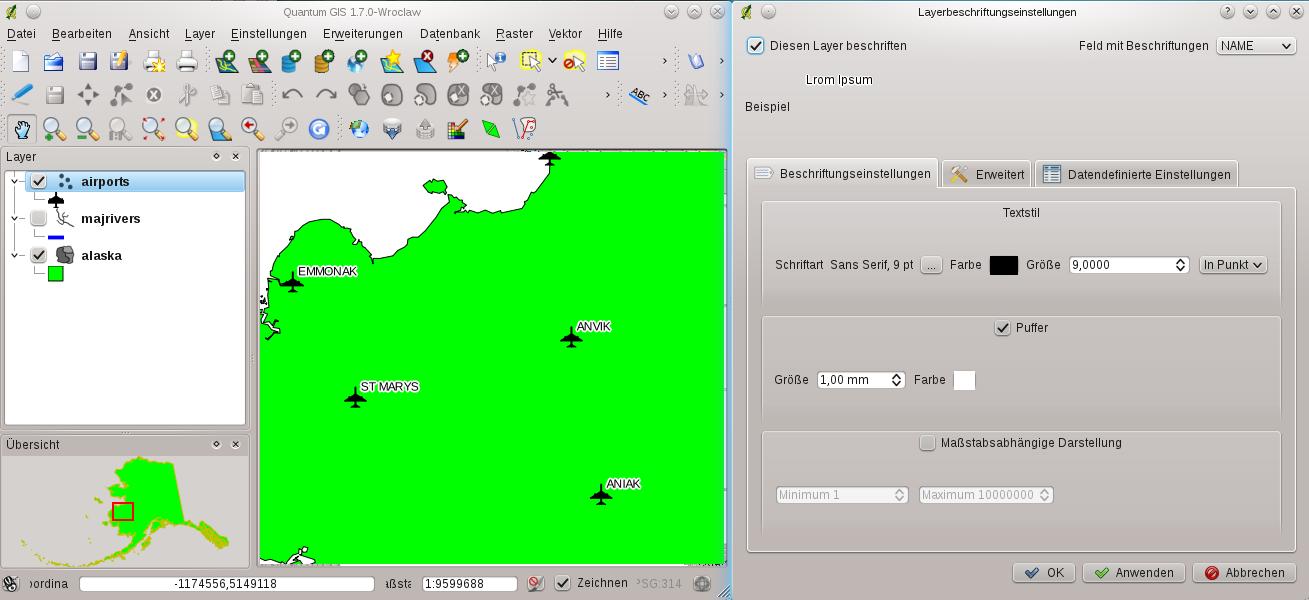
\includegraphics[clip=true, width=12cm]{label_points}
\end{center}
\end{figure}

\minisec{Linienlayer beschriften}

Als erstes m�ssen Sie das Kontrollk�stchen \checkbox{Diesen Layer beschriften}
aktivieren und eine Attributspalte angeben, deren Inhalt f�r die Beschriftung
verwendet werden soll. Danach k�nnen Sie die Platzierung, den Textstil, die
Priorit�t der Beschriftung und die Ma�stabsabh�ngige Darstellung festlegen. �ber
weitere Kontrollk�stchen k�nnen Sie noch angeben, ob alle Teile eine mehrteiligen
beschriftet werden sollen, ob sich anschlie�ende Linien verbunden werden sollen,
um doppelte Beschriftung zu vermeide und ob Objekte ein Hindernis f�r die
Beschriftung sein sollen oder nicht (siehe Abbildung \ref{fig:linelabel}).

\begin{figure}[ht]
\begin{center}
   \caption{Beschriftung von Vektor Linienlayern \nixcaption}\label{fig:linelabel}\smallskip
   \includegraphics[clip=true, width=12cm]{label_line}
\end{center}
\end{figure}

\minisec{Polygonlayer beschriften}

Als erstes m�ssen Sie das Kontrollk�stchen \checkbox{Diesen Layer beschriften}
aktivieren und eine Attributspalte angeben, deren Inhalt f�r die Beschriftung
verwendet werden soll. Danach k�nnen Sie die Platzierung, den Textstil, die
Priorit�t der Beschriftung und die Ma�stabsabh�ngige Darstellung festlegen. �ber
weitere Kontrollk�stchen k�nnen Sie noch angeben, ob alle Teile eine mehrteiligen
beschriftet werden sollen, ob Objekte ein Hindernis f�r die Beschriftung sein
sollen oder nicht (siehe Abbildung \ref{fig:arealabel}).

\begin{figure}[ht]
\begin{center}
   \caption{Beschriftung von Vektor Polygonlayern \nixcaption}\label{fig:arealabel}\smallskip
   \includegraphics[clip=true, width=12cm]{label_area}
\end{center}
\end{figure}

\minisec{Beschriftungseinstellungen �ndern}

Au�erdem k�nnen Sie auf den Knopf \button{Beschriftungseinstellungen} dr�cken und
eine Suchmethode f�r die optimale Beschriftung ausw�hlen, Zur Verf�gung steht Kette,
Popmusik Tabu, Popmusik Kette, Popmusic Tabu Kette und FALP.

\begin{figure}[ht]
\begin{center}
   \caption{�ndern der Beschriftungseinstellungen \nixcaption}\label{fig:labelengine}\smallskip
   \includegraphics[clip=true, width=7cm]{label_engine}
\end{center}
\end{figure}

Dazu k�nnen Sie noch ausw�hlen, ob alle Beschriftungskandidaten angezeigt werden
sollten (zur Fehlerbeseitigung) oder ob alle Beschriftungen dargestellt werden
sollen, also inklusive der kollidierenden.

\minisec{Schl�sselworte f�r Beschriftung in der Attributspalte}

Es gibt eine Reihe von Schl�sselworten, die verwendet werden k�nnen, um die 
Platzierung von Beschriftungen mittels einer Attributspalte festzulegen.

\begin{itemize}[label=--]
\item \textbf{F�r horizontale Ausrichtung}: left, center, right
\item \textbf{F�r vertikale Ausrichtung}: bottom, base, half, top
\item \textbf{Farben k�nnen mit SVG Angaben definiert werden}, z.B. \#ff0000
\item \textbf{f�r Fett, Unterstrichen, Durchgestrichen und Kursiv gilt}: 0 = false 1 = true
\end{itemize}

Eine Kombination von of Schl�sselworten funktioniert auch, z.B.: base right oder bottom left.

\subsection{Attribute}\index{Attribute}\label{label_attributes}

Innerhalb des Reiters \tab{Attribute} kann die Eingabe von Attributwerten f�r
den Layer beinflusst werden. Aktuell k�nnen nur PostGIS-Layer editiert
werden, da diese Funktion noch nicht durch GDAL/OGR unterst�tzt wird. Wenn
Sie auf den Knopf \toolbtntwo{mActionToggleEditing}{Bearbeitungsmodus
umschalten} klicken, k�nnen Sie f�r PostGIS Daten auch die Kn�pfe
\toolbtntwo{mActionNewAttribute}{Neue Attributspalte} und
\toolbtntwo{mActionDeleteAttribute}{L�sche Attributspalte} nutzen. Das
Hinzuf�gen einer neuen Attributspalte wird dabei nur unterst�tzt, wenn die
auf ihrem Rechner installierte GDAL Version >= 1.6 ist. Im GDAL/OGR Bugtracker 
befindet sich noch ein Patch (Ticket 2671), der darauf wartet eingef�gt zu 
werden, um eine Attributspalte zu l�schen. Solange k�nnen Sie das externe 
Python Plugin 'Table Manager' dazu verwenden.

\minisec{Feld zur Definition eines Bearbeitungselements f�r eine Attributspalte}

\begin{figure}[H]
   \begin{center}
   \caption{Dialog, um ein Bearbeitungselement f�r eine Attributspalte
auszuw�hlen \nixcaption}\label{fig:editwidget}\smallskip
   \includegraphics[clip=true, width=14cm]{editwidgetsdialog}
\end{center}
\end{figure}

Innerhalb des des Reiters \tab{Attribute} gibt es auch ein Feld
\usertext{Bearbeitungselement}. Dieses Feld kann verwendet werden, um Werte
oder Wertebereiche zu definieren, die w�hrend des Editierens einer bestimmten
Attributspalte erlaubt sind. Auf Grundlage der Eintr�ge werden
unterschiedliche Eingabefenster w�hrend des Editierens erstellt:

\begin{itemize}[label=--]
\item \textbf{Eingabezeile}: Eingabefeld f�r einfachen Text oder numerische Attribute.
Dies ist der Standard.
\item \textbf{Klassifikation}: Auswahlliste mit den Attributwerten, die im Reiter
\tab{Stil} als Legendentyp 'Eindeutiger Wert' f�r die Klassifikation
benutzt werden.
\item \textbf{Bereich}: Erlaubt die Eingabe von Werten eines gegebenen Bereichs sowie
der Schrittweite. Das Bearbeitungselement kann dabei entweder als Schieber
oder als Drehfeld dargestellt werden.
\item \textbf{Eindeutige Werte}: Der Benutzer kann einen Wert w�hlen, der bereits in
dem Attribut verwendet wird. Wenn \checkbox{�nderbar} ausgew�hlt wird, wird
eine Eingabezeile mit Autovervollst�ndigung angezeigt. Anderseits wird eine
Auswahlliste dargestellt.
\item \textbf{Dateiname}: Erm�glicht die Dateiauswahl durch einen Auswahldialog.
\item \textbf{Wertabbildung}: Es wird eine Auswahlliste mit vordefinierten Elementen
angezeigt. Die Eingabe im Feld Wert entspricht dabei dem Attribut, das
gespeichert wird. Der Eintrag im Feld Beschreibung wird in der Auswahlliste
angezeigt.
\item \textbf{Aufz�hlung}: Hier wird eine Auswahlliste mit Werten angezeigt, die als
Spaltentyp benutzt werden k�nnen. Der Datenprovider muss diese Funktion
unterst�tzen. Dies ist aktuell nur f�r Postgres als Datenprovider der Fall.
\item \textbf{Unver�nderbar}: In diesem Fall ist das Attribut unver�nderlich. Der
Benutzer kann es also nicht ver�ndern.
\item \textbf{Versteckt}: Eine versteckte Attributspalte ist f�r den Anwender unsichtbar. 
Der Inhalt wird ausgeblendet.
\item \textbf{Kontrollk�stchen}: Zeigt ein Kontrollk�stchen. Es kann festgelegt werden, 
welches Attribute bzw. welcher Wert eingetragen wird, wenn das Kontrollk�stchen 
aktiv oder inaktiv ist.
\item \textbf{Texteditor}: �ffnet ein Textfeld, in dem mehrzeiliger Text eingetragen werden kann.
\item \textbf{Kalender}: �ffnet ein Kalenderfenster, um ein Datum auszuw�hlen und in die 
Attributtabelle einzutragen. Der Spaltentyp muss String sein.
\end{itemize}

\subsection{Allgemein}\label{vectorgeneraltab}

Der Reiter \tab{Allgemein} im Dialog \dialog{Layereigenschaften} erm�glicht
es, den Anzeigenamen in der Legende zu ver�ndern, einen r�umlichen Index f�r
PostGIS- sowie OGR-Layer zu erstellen, das Koordinatenbezugssystem des Layers
zu definieren und einen Minimum- und Maximumwert f�r Ma"sstabsabh�ngiges
Zeichnen festzulegen. Zus�tzlich k�nnen Sie an dieser Stelle auch �ber den 
Knopf \button{IU zur Bearbeitung} ein User Interface einbinden, dass Sie selbst 
erstellen k�nnen mit den 'QT Creator IDE and Tools' Anwendungen von der URL 
\url{http://qt.nokia.com/products/developer-tools}. 

Der Knopf \button{Query Builder} erm�glicht es, SQL-Abfragen an die
Attributdaten des Layers zu richten. Dieser Knopf ist momentan nur bei
PostGIS Layern aktiv. Um den Query Builder auch auf Attributdaten von
OGR-Layern anwenden zu k�nnen, m�ssen Sie die Attributtabelle des
entsprechenden Layers �ffnen und dann auf den Knopf \button{Erweitert...}
dr�cken.

\subsection{Metadaten}

Der Reiter \tab{Metadaten} enth�lt allgemeine Informationen zu dem Layer
inklusive Angaben zu Datentyp, Datenquelle, Anzahl Objekte, Ausdehnung und
Editierm�glichkeiten. Sie finden auch Informationen zur r�umlichen Ausdehnung
und zum Koordinatenbezugssystem.

\subsection{Aktionen auf Basis von Attributen}\index{Aktionen}\label{label_actions}

QGIS bietet die M�glichkeit, Aktionen auf Basis von Attributen einer Ebene
durchzuf�hren. Dies kann f�r eine Vielzahl von Aktionen genutzt werden, z.B.
um ein Programm mit Abfragen aus der Attributdatenbank zu f�ttern oder
Ergebnisse einer Attributabfrage f�r ein statistisches Tool bereitzustellen.

Aktionen auf Basis von Attributen sind sinnvoll, wenn sie mit externen
Applikationen auf Ergebnisse einer oder mehrerer Attributabfragen von
Vektorlayern zugreifen m�chten. Ein Beispiel finden Sie im n�chsten Abschnitt.

\minisec{Aktionen definieren}\index{Aktionen!Definition}

Attribut-Aktionen werden im Dialog \dialog{Layereigenschaften} im Reiter
\texttt{Aktionen} definiert. Sie brauchen einen Namen f�r die Aktion und das
externe Programm, das w�hrend der Aktion gestartet werden soll. Sie k�nnen
ein oder mehrere Attributfelder einbinden. Alle Zeichen, die mit \% und dem
Namen eines Feldes beginnen, werden durch den Wert dieses Feldes ersetzt. Die
Spezialfelder \%\% \index{\%\%} werden ersetzt durch den Wert des Feldes, der
auf Basis von Abfrageergebnissen selektiert wird (vgl.
Abschnitt~\ref{label_usingactions}). Doppelte Anf�hrungsstriche k�nnen dazu
benutzt werden, um mehrere Worte als ein Ausdruck gruppiert zu �bergeben.
Doppelte Anf�hrungsstriche werden ignoriert, wenn davor ein Backslash steht.

Wenn in der Attributtabelle Spaltenamen auftreten, die eine Teilzeichenfolge
eines anderen Spaltenamen sind (z.B.: \usertext{Spalte1} and
\usertext{Spalte10}) sollten Sie diese Spaltenamen (und \%-Zeichen) in eckige
Klammern schreiben (z.B.: \usertext{[\%Spalte10]}. Dadurch wird verhindert,
dass die \usertext{[\%Spalte10]} Spalte interpretiert wird als
\usertext{[\%Spalte1]} und einer \usertext{0} am Ende. Die eckigen Klammern
werden von QGIS bei der Ausf�hrung entfernt. Wenn Sie m�chten, dass um den
Spaltennamen eine eckige Klammer steht, erg�nzen Sie den Ausdruck durch zwei
weitere eckige Klammern: \usertext{[[\%Spalte10]]}.

Das Dialogfenster \dialog{Abfrageergebnisse} enth�lt auch eine {\em
(abgeleitet)} Information in abh�ngigkeit vom Layertyp. Die hier angezeigten
Werte k�nnen auf �hnliche Weise eingebunden werden, wie Spalten aus der
Attributtabelle, indem vor den erfassten Wert ein \usertext{(abgeleitet).}
gestellt wird. Zum Beispiel: Ein Punktlayer zeigt Felder mit der
\usertext{X}- und \usertext{Y}-Koordinate. Diese k�nnen in der Aktion genutzt
werden mit dem Eintrag \usertext{\%(abgeleitet).X} and
\usertext{\%(abgeleitet).Y}. Diese abgeleiteten Aktionen k�nnen nur �ber den
Dialog \dialog{Abfrageergebnisse} angesprochen werden, nicht �ber
die \dialog{Attributtable}. 

Zur besseren Erl�uterung zwei Beispiele:\index{Aktionen!Beispiele}

\begin{verbatim}
    konqueror http://www.google.com/search?q=\%nam
    konqueror http://www.google.com/search?q=\%\%
\end{verbatim}

Im ersten Beispiel wird an den Webbrowser Konqueror eine Google URL
�bergeben mit dem Wert eines Feldes \usertext{nam} eines Vektorlayers.
Beachten Sie, dass sich das bei einer Aktion aufgerufene Programm im Pfad
befinden muss. Ansonsten m�ssen Sie den gesamten Pfad angeben:

\begin{verbatim}
/opt/kde3/bin/konqueror http://www.google.com/search?q=\%nam
\end{verbatim}

Das zweite Beispiel nutzt den Ausdruck \%\%, welcher unabh�ngig ist von einem
speziellen Feld. Beim Ausf�hren des Befehls wird der Ausdruck \%\% durch den
Wert des jeweils selektierten Feldes ersetzt.

\minisec{Aktionen anwenden}\index{Aktionen!anwenden}\label{label_usingactions}

Aktionen k�nnen entweder �ber den Dialog \dialog{Abfrageergebnisse} oder die
ge�ffnete \dialog{Attributtabelle} gestartet werden. Beide Dialoge sind per
Maus erreichbar �ber \toolbtntwo{mActionOpenTable}{Abfrageergebnisse} oder
\toolbtntwo{mActionOpenTable}{Attributtabelle �ffnen}.) Um eine Aktion
aufzurufen, klicken Sie mit der rechten Maustaste auf einen Eintrag in der
Attributtabelle und w�hlen die gew�nschte Aktion aus der Liste aus.

Wenn eine Aktion mit dem Ausdruck \%\% gestartet werden soll, klicken Sie mit
der rechten Maustaste auf einen Eintrag in der \dialog{Attributtabelle} oder im
Dialog \dialog{Abfrageergebnisse} und w�hlen die gew�nschte Aktion aus der
Liste aus.

In einem weiteren Beispiel soll gezeigt werden, wie Attributwerte aus eines
Vektorlayers abgefragt und in eine Textdatei mit Hilfe der Bash und des
\usertext{echo} Kommandos geschrieben werden (funktioniert also nur unter
\nix und evtl. \osx). Der Abfragelayer enth�lt die Felder Art
\usertext{taxon\_name}, Latitude \usertext{lat} und Longitude
\usertext{long}. Um eine r�umliche Abfrage eines Ortes zu erstellen und die
Werte der drei Felder in eine Textdatei zu schreiben, wird folgende Aktion
erstellt:

\begin{verbatim}
  bash -c "echo \"%taxon_name %lat %long\" >> /tmp/species_localities.txt"
\end{verbatim} 

Nachdem ein paar Orte auf dem Bildschirm ausgew�hlt wurden (diese erscheinen
gelb hinterlegt), starten wir die Aktion mit der rechten Maustaste �ber den
Dialog \dialog{Abfrageergebnisse} und k�nnen danach in der Textdatei die
Ergebnisse ansehen:

\begin{verbatim}
  Acacia mearnsii -34.0800000000 150.0800000000
  Acacia mearnsii -34.9000000000 150.1200000000
  Acacia mearnsii -35.2200000000 149.9300000000
  Acacia mearnsii -32.2700000000 150.4100000000
\end{verbatim} 

Als �bung erstellen wir eine Aktion, bei der Google nach dem Namen des
jeweiligen Sees in dem Layer \filename{lakes} sucht. Als erstes geben wir die
URL ein, die wir brauchen, um auf Basis eines Schl�sselwortes zu suchen. Das
ist einfach, in dem wir einfach auf der Google Webseite nach einem Begriff
suchen und die URL dann kopieren. Das Format, das wir brauchen ist:
\url{http://google.com/search?q=qgis}, wobei \usertext{qgis} das
Schl�sselwort ist, nach dem wir suchen wollen. Nun kann es weiter gehen:

\begin{itemize}[label=--]
\item Laden Sie den Layer \filename{lakes.shp}
\item �ffnen Sie die \dialog{Layereigenschaften} Dialog, indem Sie doppelt
auf den Layernamen \filename{lakes} in der Legende klicken oder w�hlen Sie
das Men� \dropmenuopt{Eigenschaften} mit der rechten Maustaste.
\item Klicken Sie auf den Reiter \tab{Aktionen}
\item Geben Sie einen Namen f�r die Aktion ein, z.B: \usertext{Google Search}
\item F�r diese Aktion ist es notwendig, den Namen des externen Programms
anzugeben, mit  dem wir das Ergebnis anzeigen lassen wollen. In unserem Fall
w�hlen wir Firefox als Webbrowser.
\item Hinter dem Namen des Programms geben wir die URL ein, die wir f�r die
Internetsuche benutzen wollen, aber ohne das Schl�sselwort:
\url{http://google.com/search?q=}
\item Der Text im Feld \guilabel{Aktion} sollte nun folgenderma�en aussehen:\\
\usertext{firefox http://google.com/search?q=}
\item Klicken Sie nun auf die Drop-Down Box mit den Spaltennamen der
Attributtabelle des Layers \filename{lakes}. Der Knopf ist gleich links neben
dem Knopf \usertext{Attribut einf�gen}.
\item W�hlen Sie die Attributspalte \selectstring{Spalte}{NAMES} und klicken auf
\button{Attribut einf�gen}.
\item Die Aktion sieht nun so aus:\\ \usertext{firefox
  http://google.com/search?q=\%NAMES}
\item Abschlie�end dr�cken Sie auf \button{Aktion hinzuf�gen}.
\end{itemize}

Damit ist die Aktion fertig f�r den Einsatz. Der gesamte Befehl der Aktion
sollte folgenderma�en aussehen:

\usertext{firefox \url{http://google.com/search?q=\%NAMES}}

Wir k�nnen die Aktion nun benutzen. Schlie�en Sie den \dialog{Eigenschaften}
Dialog und zoomen Sie in eine Bereich ihrer Wahl mit ein paar Seen. Stellen Sie
sicher, dass der Layer \filename{lakes} in der Legende aktiviert ist. Nun
identifizieren Sie einen See. In der Ergebnisanzeige sollte nun die Aktion
sichtbar sein:

\begin{figure}[H]
   \begin{center}
   \caption{Ausw�hlen eines Objektes mit einer Aktion \nixcaption}
   \label{fig:identify_action}\smallskip
   \includegraphics[clip=true, width=6cm]{action_identifyaction} 
\end{center}  
\end{figure}

Wenn wir nun auf das Wort \usertext{action} klicken, �ffnet sich der
Webbrowser Firefox und zeigt uns das Ergebnis der Internetrecherche z.B. nach
dem See Tustumena an \url{http://www.google.com/search?q=Tustumena}. Es ist
�brigens auch m�glich, weitere Attributspalten zu erg�nzen. Dazu f�gen Sie
einfach ein ``+''-Zeichen an das Ende der Aktion, w�hlen eine weitere
Attributspalte und klicken wieder auf den Knopf \texttt{Attribut einf�gen}.
In unserem Datensatz ist leider keine weitere sinnvolle Attributspalte
vorhanden, nach der man im Internet suchen k�nnte.

Sie k�nnen auch mehrere Aktionen f�r einen Layer definieren. Sie alle werden
dann bei der Abfrage von Objekten im Dialog \dialog{Abfrageergebnisse}
angezeigt und k�nnen ausgew�hlt und benutzt werden. 

Sie sehen, man kann sich eine Vielzahl interessanter Aktionen ausdenken. Wenn
Sie z.B. einen Punktlayer mit einzelnen Punkten haben, an denen Photos
geschossen wurden, dann k�nnen Sie eine Aktion erstellen, �ber die Sie dann
das entsprechende Photo anzeigen lassen k�nnen, wenn Sie auf den Punkt in der
Karte klicken. Man kann auch zu bestimmten Attributen webbasierte
Information ablegen (z.B. in einer HTML-Datei) und diese dann
�ber eine Aktion anzeigen lassen, etwa so wie in dem Google Beispiel.

\subsection{Verkn�pfungen}\label{sec:joins}
\index{Vektorlayer!Verkn�pfungen}

Der Reiter \tab{Verkn�pfungen} erm�glicht es, eine in QGIS geladene Attributtabelle 
mit einem Vektorlayer zu verkn�pfen. Im Dialog \dialog{Verkn�pfung hinzuf�gen} w�hlen 
Sie eine Attributtabelle als Layer aus, ein darin enthaltene Verkn�pfungsfeld und 
das dazu passende Zielfeld im Vektorlayer. QGIS erlaubt die Verkn�pfung mit 
Datenformaten, die von OGR und PostgreSQL unterst�tzt werden sowie ASCII Tabellen, 
die mit dem Plugin 'Textdatei als Layer importieren' gelesen wurden.

Zus�tzlich stehen noch folgende Funktionen zur Auswahl:

\begin{itemize}[label=--]
\item \checkbox{Verkn�pfung im Speicher cachen}
\item \checkbox{Index auf Feld erzeugen}
\end{itemize}

\subsection{Diagramme}\label{sec:diagram}
\index{Vektorlayer!Diagram Overlay}

Der Reiter \tab{Diagramme} erm�glicht es, ein Diagramm als Grafik �ber
einen Vektorlayer zu visualisieren (siehe Abbildung~\ref{fig:diagramtab}). 

\begin{figure}[ht]
   \begin{center}
   \caption{Vektor Layereigenschaften mit Diagramm �berlagerung \nixcaption}
   \label{fig:diagramtab}\smallskip
   \includegraphics[clip=true, width=13cm]{diagram_tab}
\end{center}
\end{figure}

Die aktuelle Implementierung des Moduls erm�glicht es, Kuchen- und Textdiagramme 
auf Basis von Attributspalten zu erstellen, und die Gr��e der Diagramme entsprechend 
einer Klassifikation linear zu skalieren. Die Anordnung der Diagramme findet in 
Abstimmung mit der neuen Beschriftung statt. Als Beispiel sollen auf dem Hintergrund 
des Layers \filename{alaska.shp} Kuchendiagramme mit Temperaturwerten gezeichnet werden. 
Die Werte daf�r entnehmen wir der Attributtabelle des Vektorlayers 
\filename{climate.shp}. Beide Layer sind Teil des QGIS Beispieldatensatzes 
(siehe Kapitel~\ref{label_sampledata}).   

\begin{enumerate}
\item Als erstes klicken Sie auf das Icon
\toolbtntwo{mActionAddOgrLayer}{Vektorlayer hinzuf�gen}, dann browsen Sie zum QGIS
Beispieldatensatz und laden die beiden Vektorlayer \filename{alaska.shp}
und \filename{climate.shp}.
\item Doppelklicken Sie auf den \filename{climate} Layer in der
Kartenlegende, um den Dialog \dialog{Layereigenschaften} zu starten.
\item Klicken Sie auf den Reiter \tab{Diagramme} und w�hlen Sie
\button{Kuchendiagramm} als Diagrammtyp.
\item Im Diagramm wollen wir die Werte von drei Attributspalten 
\filename{T\_F\_JAN, T\_F\_JUL} und \filename{T\_F\_MEAN} anzeigen. Als
erstes selektieren wir \filename{T\_F\_JAN} als Attribute und klicken auf
\button{Attribute hinzuf�gen}, dann \filename{T\_F\_JUL} und schlie�lich
\filename{T\_F\_MEAN}.
\item Zum linearen Skalieren der Diagrammgr��e definieren wir \filename{T\_F\_JUL}
als Klassifikationsattribut.
\item Nun klicken wir auf \button{Maximalwert suchen}, w�hlen den Wert 10 f�r
die Gr��e und die Gr��eneinheit und klicken auf \button{Anwenden}, um die
Diagramme in QGIS anzuzeigen.
\item Sie k�nnen nun die Gr��e weiter anpassen oder die Farben �ndern, 
indem Sie auf die Farbe des Attributs doppelklicken und dann eine entsprechende 
Farbe ausw�hlen. Abbildung~\ref{fig:climatediagram} gibt einen ersten Eindruck.
\item Abschlie�end klicken Sie \button{Ok}.
\end{enumerate}

\begin{figure}[ht]
   \begin{center}
   \caption{Kuchendiagramm mit Temperaturdaten vor dem Hintergrund des Alaska Layers \nixcaption}\label{fig:climatediagram}\smallskip
   \includegraphics[clip=true, width=13cm]{climate_diagram}
\end{center}
\end{figure}

\section{Editierfunktionen}\index{Editierfunktionen}

QGIS bietet einfache Editierfunktionen f�r Vektordaten. Bevor Sie
weiterlesen sollten Sie sich bewusst sein, dass derzeit nicht alle
Funktionen ausgereift sind. Bevor Sie also anfangen, Vektorlayer zu
editieren, sollten Sie die Daten sichern.

\textbf{Bemerkung}: Die Vorgehensweise zum Editieren von GRASS Vektorlayern
ist anders und wird in Kapitel~\ref{grass_digitising} beschrieben.

\begin{Tip}[h]\caption{\textsc{Zeitgleiches Editieren}}
Diese QGIS Version kontrolliert nicht, ob zwei Personen gleichzeitig
an einem Vektorlayer arbeiten. Die zuletzt schreibende Person gewinnt.
\end{Tip}

\subsection{Einstellen der Fangtoleranz und des Suchradius}

bevor wir damit beginnen k�nnen, Vektorgeometrien zu editieren, ist es sehr
wichtig die Fangtoleranz und den Suchradius f�r St�tzpunkte (Vertices)
festzulegen, um optimale Ergebnisse zu erzielen. 

\minisec{Fangtoleranz}

Die Fangtoleranz ist der Abstand, den QGIS verwendet, um beim digitalisieren den
n�chstgelegenen St�tzpunkt bzw. das n�chstgelegene Liniensegment zu suchen
und sich damit zu verbinden. Die Fangtoleranz beeinflusst alle Werkzeuge, die
mit einer Fangtoleranz arbeiten. Wenn Sie sich nicht innerhalb der definierten
Fangtoleranz befinden, wird der St�tzpunkt dort gesetzt, wo sich der
Mauszeiger gerade befindet, wenn Sie die Maustaste dr�cken, ohne darauf zu
achten, dass Linienz�ge und Fl�chen geschlossen sind. Es gibt zwei
M�glichkeiten, die Fangtoleranz einzustellen:

\begin{enumerate}
\item Ein allgemeiner, projektweiter Fangmodus kann im Men�
\mainmenuopt{Einstellungen} \arrow \dropmenuopttwo{mActionOptions}{Optionen}
eingestellt werden. (Unter Mac klicken Sie \mainmenuopt{QGIS} \arrow
\dropmenuopttwo{mActionOptions}{Optionen}). Im Reiter \tab{Digitalisierung}
k�nnen Sie ausw�hlen, ob sich der Fangmodus auf St�tzpunkte, Segmente oder
auf St�tzpunkte und Segmente beziehen soll. Sie k�nnen auch in Layereinheiten
definieren, ob die Fangtoleranz oder der Suchradius in Karteneinheiten oder
Pixeln berechnet werden soll. Die Einstellung Pixel hat dabei den Vorteil, dass die
Fangtoleranz nicht ver�ndert werden muss, wenn der Ma�stab ge�ndert wird, Sie
also hinein- oder herauszoomen. Wenn Sie mit den Alaska-Daten arbeiten
bezieht sich die Layereinheit auf \usertext{feet} und ein Wert von etwa 300ft
bei einem Ma�stab 1:10 000 sollte f�r die �bungen gut funktionieren.
\item Eine Layer-basierter Fangmodus kann festgelegt werden im Men�
\mainmenuopt{Einstellungen} \arrow \mainmenuopt{Fangoptionen}. F�r jeden in 
QGIS geladenen Vektorlayer kann Fangmodus und Fangtoleranz eingestellt, 
aktiviert oder deaktiviert werden (vgl. Abbildung~\ref{fig:snappingoptions}). 
Diese layerbasierte Einstellung �berschreibt die globalen Einstellungen, die 
Sie im Reiter \tab{Digitalisierung} unter \mainmenuopt{Einstellungen} \arrow 
\mainmenuopt{Optionen} definiert haben. Wenn Sie also einen Layer editieren
und auf die Geometrien eines anderen Layers snappen wollen, dann aktivieren
Sie die Fangoptionen nur f�r diesen Layer und setzen Sie die globale
Fangtoleranz auf einen kleineren Wert. Die Fangtoleranz wird nur auf
ausgew�hlte Layer angewendet, unabh�ngig von der globalen Fangtoleranz.
Vergewissern Sie sich daher, dass die Layer, auf die Sie snappen wollen, auch
im Dialog Fangoptionen ausgew�hlt sind.  
\end{enumerate}

\begin{figure}[H]
   \begin{center}
   \caption{Fangmodus und -toleranz der Vektorlayer einstellen \nixcaption}\label{fig:snappingoptions}\smallskip
   \includegraphics[clip=true, width=14cm]{editProjectSnapping} 
\end{center}  
\end{figure}

\minisec{Suchradius}

Der Suchradius ist die Distanz, mit der QGIS die n�chstgelegenen St�tzpunkte
zum Mauszeiger findet. Wenn der Mauszeiger sich nicht innerhalb des Suchradius
befindet, wird kein St�tzpunkt gefunden, solange Sie nicht wirklich
direkt auf einen treffen, um diesen z.B. zu verschieben, zu l�schen oder
anderweitig zu editieren. Beide Parameter, Fangtoleranz und Suchradius sind
in Layereinheiten zu definieren und es kann gut sein, dass Sie f�r ihre
Anspr�che ein wenig mit den Werten experimentieren m�ssen. Dies gilt
besonders, wenn es eine gro�e Anzahl von St�tzpunkten auf kleiner Fl�che
sind. 

Der Suchradius zum Editieren von St�tzpunkten kann eingestellt werden im
Reiter \tab{Digitalisierung} des Men�s \mainmenuopt{Einstellungen} \arrow
\dropmenuopttwo{mActionOptions}{Optionen}. Derselbe Ort, an dem auch die
Fangtoleranz und der Fangmodus definiert werden.  

\subsection{Zoomen und Karte verschieben}

Bevor Sie einen Layer editieren, sollten Sie in den Bereich hineinzoomen, den
Sie bearbeiten wollen. Dadurch vermeiden Sie lange Wartezeiten, bis alle
St�tzpunkte des Layers visualisiert werden.

Die Werkzeuge \toolbtntwo{mActionPan}{Karte verschieben} und
\toolbtntwo{mActionZoomIn}{Hineinzoomen}/\toolbtntwo{mActionZoomOut}{Herauszoomen},
k�nnen nicht nur �ber diese Icons verwendet werden. Die Navigation innerhalb
einer Karte kann auch mit dem Mausrad, den Bildtasten, der Leertaste und den
Pfeiltasten durchgef�hrt werden.

\minisec{Mit dem Mausrad im Kartenfenster zoomen und verschieben}

W�hrend des Digitalisierens k�nnen Sie auf das Mausrad dr�cken und dann
gleichzeitig das
Kartenfenster verschieben. Oder Sie k�nnen das Mausrad drehen, um im
Kartenfenster hinein- und hinauszuzoomen. Zum Zoomen platzieren Sie den
Mauszeiger auf einen Kartenbereich und drehen dann das Mausrad nach vorne
(weg von Ihnen) zum Hineinzoomen oder nach hinten (n�her an Sie heran) zum
Hinauszoomen bewegen. Die Position des Mauszeigers ist dabei das Zentrum des
Zoomvorgangs. Sie k�nnen das Zoomberhalten des Mausrades in dem Reiter
\tab{Kartenwerkzeuge} des Men�s \mainmenuopt{Einstellungen} \arrow
\dropmenuopt{Optionen} ver�ndern.

\minisec{Den Layer mit den Pfeiltasten im Kartenfenster verschieben}

Das Verschieben des Layers im Kartenfenster w�hrend des Digitalisierens ist
mit den Pfeiltasten m�glich. Plazieren Sie den Mauszeiger in das
Kartenfenster und dr�cken Sie rechte Pfeiltaste, um den Layer nach Osten zu
verschieben, die linke Pfeiltaste f�r Westen, die Pfeiltaste nach unten f�r
S�den und die Pfeiltaste nach oben f�r das Verschieben nach Norden.

Sie k�nnen auch die gedr�ckte Leer-Taste dazu verwenden, um den Layer im
Kartenfenster zu verschieben, wenn Sie mit dem Mauszeiger dar�bergehen. Die
Leer-Taste �bernimmt dabei die Aufgabe der linken Maustaste. Zum Hinein- und
Herauszoomen k�nnen Sie �brigens auch die \keystroke{BildHoch} und
\keystroke{BildRunter} Tasten verwenden, so wie Sie es ansonsten mit dem
Mausrad tun k�nnen.

All diese Funktionen erm�glichen es Ihnen, in einem Layer zu zoomen oder
diesen zu verschieben, ohne das Sie das Digitalisieren unterbrechen m�ssen.

\subsection{Topologisches Editieren}

Abgesehen von der Einstellung des Layer-basierten Fangmodus k�nnen im Men�
\mainmenuopt{Einstellungen} \arrow \mainmenuopt{Fangoptionen} auch topologische
Funktionen aktiviert werden. Hier k�nnen Sie allgemein 
\checkbox{Topologisches Editieren an} ausw�hlen und/oder f�r jeden Layer einzeln ein Kontrollk�stchen in der Spalte \checkbox{�berschneidung vermeiden} aktivieren.

\minisec{Erm�gliche topologisches Editieren}

Das Kontrollk�stchen \checkbox{Topologisches Editieren an} unterst�tzt das 
Editieren und Kontrollieren gemeinsamer Grenzlinien in Polygon-Layern. QGIS 
'erkennt' gemeinsame Fl�chengrenzen und beim Verschieben des St�tzpunktes 
einer Fl�che werden dann automatisch die anderen Fl�chengrenzen angepasst 
und mit verschoben.

\minisec{�berschneidung vermeiden}

Als zweite topologische Funktion gibt es ein Kontrollk�stchen in der Spalte
\checkbox{�berschneidung verm.}. Damit wird es vereinfacht,
angrenzende Polygone zu digitalisieren. Wenn bereits ein Polygon digitalisiert
wurde, kann das zweite auch mit einer �berlagerung des ersten Polygons
erstellt werden und QGIS schneidet dann die �berlagerungen weg, so dass die
Fl�chen exakt aneinander liegen. Der Vorteil ist, dass nicht alle St�tzpunkte
einer gemeinsamen Grenzlinie digitalisiert werden m�ssen.

\subsection{Einen vorhandenen Layer editieren}
\index{Vektorlayer!Editierfunktionen}
\index{Editierfunktionen!existierender Layer}
\label{sec:edit_existing_layer}

Standardm��ig l�dt QGIS Vektorlayer im 'read-only' Modus, um ungewolltes
Editieren zu verhindern. Ansonsten k�nnen aber alle Ebenen editiert werden,
wenn es der Datenanbieter erlaubt bzw. die Rechte entsprechend gesetzt sind.
Das Editieren von Vektorlayern ist am vielseitigsten bei PostgreSQL/PostGIS
Daten. 

Das Editieren von Vektorlayern in QGIS ist unterteilt in Digitalisierung und
erweiterte Digitalisierung, siehe Kapitel \ref{sec:advanced_edit}. Beide
Werkzeugleisten k�nnen �ber das Men� \mainmenuopt{Einstellungen} \arrow
\dropmenuopt{Werkzeugk�sten} aktiviert und deaktiviert werden. Mit der
Werkzeugleiste Digitalisierung k�nnen folgende Funktionen ausgef�hrt werden:

\begin{table}[h]\index{Vektorlayer!Grundlegende Editierwerkzeuge}
\centering
\caption{Funktionen der Werkzeugleiste Digitalisierung}
\label{tab:vector_editing}
\begin{tabular}{|l|p{6.9cm}|l|p{6.9cm}|}
\hline \textbf{Icon} & \textbf{Funktion} & \textbf{Icon} & \textbf{Funktion} \\
\hline \includegraphics[width=0.7cm]{mActionToggleEditing}
   & Bearbeitungsstatus umschalten
   & \includegraphics[width=0.7cm]{mActionCapturePoint}
   & Objekte Digitalisieren: Punkt hinzuf�gen \\
\hline \includegraphics[width=0.7cm]{mActionCaptureLine}
   & Objekte Digitalisieren: Linie hinzuf�gen
   & \includegraphics[width=0.7cm]{mActionCapturePolygon}
   & Objekte Digitalisieren: Polygon hinzuf�gen \\
\hline \includegraphics[width=0.7cm]{mActionMoveFeature}
   & Objekt verschieben
   & \includegraphics[width=0.7cm]{mActionNodeTool}
   & Knotenwerkzeug \\
\hline \includegraphics[width=0.7cm]{mActionDeleteSelected}
   & Ausgew�hltes l�schen
   & \includegraphics[width=0.7cm]{mActionEditCut}
   & Ausgew�hlte Objekte ausschneiden \\
\hline \includegraphics[width=0.7cm]{mActionEditCopy}
   & Objekte kopieren
   & \includegraphics[width=0.7cm]{mActionEditPaste} 
   & Objekte einf�gen \\
\hline \includegraphics[width=0.7cm]{mActionFileSave}
   & �nderungen speichern
   & & \\
\hline
\end{tabular}
\end{table}

\begin{Tip}[h]\caption{\textsc{Daten-Integrit�t}}
Bitte beachten Sie, Daten vor und w�hrend des Editierens regelm��ig
zu sichern, um bei Fehlern keine unn�tigen Verluste zu erleiden. Auch wenn
QGIS mittlerweile sehr stabil ist, was die Daten-Integrit�t betrifft, sollten
Sie sich nicht darauf verlassen
\end{Tip}

\begin{Tip}[ht]\caption{\textsc{Regelm��iges Sichern der Daten}}
Bitte speichern Sie ihre Arbeit regelm��ig mit dem Knopf
\toolbtntwo{mActionFileSave}{�nderungen Speichern}. Dadurch wird 
sichergestellt, dass die aktuellen �nderungen auch akzeptiert werden.
\end{Tip}

\begin{Tip}[h]\caption{\textsc{Zoomen zum letzten Editierstand}}
Vor dem Editieren eines Vektorlayers sollten Sie in den Bereich
zoomen, den Sie ver�ndern m�chten. Dadurch wird die zeitaufwendige
Darstellung s�mtlicher Knotenpunkte des Vektorlayers im Kartenfenster
verhindert.
\end{Tip}

\begin{Tip}[h]\caption{\textsc{St�tzpunktsymbol �ndern}}
QGIS erm�glicht es, das Symbol f�r die St�tzpunkte zu ver�ndern. Sie
k�nnen w�hlen zwischen einem Kreuz und einem halbtransparenten Kreis. Zum
�ndern gehen Sie in das Men� \mainmenuopt{Einstellungen} \arrow
\dropmenuopttwo{mActionOptions}{Optionen} und w�hlen im Reiter
\tab{Digitalisierung} das entsprechende Symbol. 
\end{Tip}

Vor jedem Editieren eines Vektorlayers muss dieser in der Legende ausgew�hlt
werden und die Option
\dropmenuopttwo{mActionToggleEditing}{Bearbeitungsstatus umschalten} in der
Werkzeugleiste aktiviert sein. Alternativ k�nnen Sie dazu auch mit der
rechten Maustaste auf den Namen des Layers in der Legende klicken und die
Option im Kontextmen� ausw�hlen. Sobald der Layer im Bearbeitungsstatus ist,
erscheinen die St�tzpunkte als das von Ihnen gew�hlte St�tzpunktsymbol und
zus�tzlich werden die Digitalisier-Tools in der Werkzeugleiste
aktiv.\index{Editierfunktionen!Icons}

\minisec{Objekte digitalisieren}
\index{Vektorlayer!Digitalisieren!Objekt}

Bevor Sie mit dem Digitalisieren von Objekten beginnen, benutzen Sie die Tools
\toolbtntwo{mActionPan}{Karte verschieben} und 
\toolbtntwo{mActionZoomIn}{Hineinzoomen}/\toolbtntwo{mActionZoomOut}{Hinauszoomen},
um sich dem Bereich zu n�hern, den Sie ver�ndern m�chten.

Danach k�nnen Sie mit den Icons \toolbtntwo{mActionCapturePoint}{Punkt
digitalisieren}, \toolbtntwo{mActionCaptureLine}{Linie digitalisieren} oder
\toolbtntwo{mActionCapturePolygon}{Polygon digitalisieren} in der
Werkzeugleiste den Mauszeiger in den Digitalisiermodus bringen.

F�r jedes Objekt wird erst die Geometrie digitalisiert und dann das Attribut
hinzugef�gt. Um eine Geometrie zu digitalisieren, klicken Sie mit der linken
Maustaste an eine gew�nschte Stelle im Kartenfenster, um den ersten Punkt zu
erstellen.

F�r Linien und Polygone klicken Sie f�r jeden weiteren Knotenpunkt wieder die
linke Maustaste. Zum Beenden klicken Sie irgendwo im Kartenfenster auf die
rechte Maustaste, um anzuzeigen, dass die Geometrie ihres Objektes fertig
gestellt ist. Dadurch wird das Attributfenster ge�ffnet und erm�glicht die
Attribute f�r das neue Objekt einzutragen. In Abbildung
\ref{fig:vector_digitising} ist ein Beispiel f�r einen fiktiven Fluss in
Alaska gezeigt. Im Reiter \tab{Digitalisierung} des Men�s \mainmenuopt{Einstellungen} 
\arrow \dropmenuopt{Optionen} k�nnen auch die Kontrollk�stchen \checkbox{Eingabe der 
Attributwerte bei der Erstellung neuer Objekte unterdr�cken} und 
\checkbox{Letzte Attributwerteingaben wiederverwenden} aktiviert werden.

\begin{figure}[ht]
   \begin{center}
   \caption{Eingabe von Attributen nach dem Digitalisieren eines neuen Objektes \nixcaption}\label{fig:vector_digitising}\smallskip
   \includegraphics[clip=true, width=8cm]{editDigitizing}
\end{center}  
\end{figure}

\begin{Tip}[h]\caption{\textsc{Datentyp der Attribute}}
QGIS kontrolliert beim Editieren von Shapes, ob die eingetragenen
Werte dem Datentyp der Attributspalte entspricht (z.B.: Zahl oder Text).
Ansonsten ist es nicht m�glich, im Dialog \dialog{Attributwert eingeben}
eine Zahl in eine Textspalte einzutragen, oder umgekehrt. Falls es dennoch
notwendig sein sollte, k�nnen Sie es nachtr�glich im Fenster der
\dialog{Attributtabelle} �ndern.
\end{Tip}

\minisec{Objekte verschieben}
\index{Vektorlayer!verschieben!Objekt}

Mit dem Werkzeug \toolbtntwo{mActionMoveFeature}{Objekte verschieben} k�nnen Sie
komplette Objekte verschieben.

\minisec{Knotenwerkzeug}
\index{Vektorlayer!Knotenwerkzeug}

F�r PostGIS und Shapedaten erm�glich das \toolbtntwo{mActionNodeTool}{Knotenwerkzeug}, 
die St�tzpunkte von Objekten zu manipulieren, �hlich wie ein CAD-Programm. Dazu
kann man mehrere St�tzpunkte gemeinsam selektieren, um sie dann zusammen zu
verschieben, zu l�schen oder hinzuzuf�gen. Das Knotenwerkzeug funktioniert
auch mit angeschalteter OTF-Projektion und unterst�tzt die Funktionen f�r
topologisches Editieren. Anders als die anderen Editierfunktionen, bleibt die
Auswahl f�r die Ver�nderungen des Objektes bestehen. Wenn das Knotenwerkzeug kein 
Objekt findet, wird eine Warnung angezeigt.

Sie sollten den Suchradius beim Digitalisieren �ber die Men�leiste unter
\mainmenuopt{Einstellungen} \arrow \dropmenuopttwo{mActionOptions}{Optionen} 
\arrow \tab{Digitalisierung} gr��er 0 einstellen. Ansonsten ist QGIS nicht in der
Lage, ein Objekt auszuw�hlen.

\minisec{Eine einfache �bung}

Beginnen Sie, indem Sie das \toolbtntwo{mActionNodeTool}{Knotenwerkzeug} aktivieren 
und dann ein Objekt selektieren. Rote Boxen erscheinen an jedem St�tzpunkt des 
Objektes. Nun sind folgende Funktionen vorhanden:

\begin{itemize}[label=--]
\item \textbf{St�tzpunkte ausw�hlen}: Das Ausw�hlen ist einfach.
Klicken Sie auf einen St�tzpunkt und die Farbe der Box wechselt nach
Blau. Sie k�nnen mehrere St�tzpunkte ausw�hlen, indem Sie die Tasten
\keystroke{Umschalt} gedr�ckt halten. Mit der Taste \keystroke{Strg} kann die
Auswahl umgekehrt werden (selektierte St�tzpunkte werden deselektiert, nicht
ausgw�hlte St�tzpunkte werden ausgew�hlt). Es ist auch m�glich, mehrere
St�tzpunkte auszuw�hlen, indem Sie ein Rechteck mit der Maus aufziehen. Alle
St�tzpunkte innerhalb des Rechtecks werden dann selektiert. Oder Sie klicken
auf eine Grenzlinie und beide angrenzenden St�tzpunkte werden selektiert.
\item \textbf{St�tzpunkte hinzuf�gen}: Dazu klicken Sie doppelt in die N�he
einer Grenzlinie und ein neuer St�tzpunkt erscheint. Beachten Sie, dass der
St�tzpunkt auf der Grenzlinie erscheint, und nicht an der Stelle, wo der
Mauspfeil ist.
\item \textbf{St�tzpunkte l�schen}: W�hlen Sie dazu St�tzpunkte aus, die
gel�scht werden sollen und klicken Sie dann auf die Taste
\keystroke{Entfernen}. Beachten Sie, dass eine Mindestanzahl St�tzpunkte f�r
den jeweiligen Objekttyp nicht gel�scht wird. Wenn Sie ein komplettes Objekt
l�schen wollen, nutzen Sie das entsprechende Werkzeug.
\item \textbf{St�tzpunkte verschieben}: W�hlen Sie alle St�tzpunkte aus, die
verschoben werden sollen. Alle ausgew�hlten St�tzpunkte werden in dieselbe
Richtung wie der Mauspfeil verschoben. Wenn eine Fangtolerazt eingestellt
ist, k�nnen die St�tzpunkte zu dem n�chstgelegenen St�tzpunkt oder Segment
snappen.
\end{itemize}

Jede Ver�nderung mit dem Knotenwerkzeug wird als einzelner Eintrag im Dialog 
\dialog{R�cknahme/Wiederholung} abgelegt und unterst�tz die topologischen 
Funktionen. Ausserdem wird On-The-Fly Reprojektion wird unterst�tzt und Sie 
k�nnen St�tzpunkte identifizieren, wenn Sie mit der Maus dr�berfahren.

\minisec{Objekte ausschneiden, kopieren und einf�gen}
\index{Vektorlayer!Objekte ausschneiden}
\index{Vektorlayer!Objekte kopieren}
\index{Vektorlayer!Objekte einf�gen}
\index{Editierfunktionen!Objekte ausschneiden}
\index{Editierfunktionen!Objekte kopieren}
\index{Editierfunktionen!Objekte einf�gen}

Ausgew�hlte Objekte k�nnen ausgeschnitten, kopiert und an andere Ebenen im
aktuellen QGIS-Projekt �bergeben (eingef�gt) werden, wenn sich der Ziellayer
auch im Editiermodus befindet, indem Sie nach Auswahl des Ziellayers auf den
Knopf \toolbtntwo{mActionToggleEditing}{Bearbeitungsstatus umschalten}
klicken.

Objekte k�nnen auch als Text an externe Applikationen �bergeben werden: Dabei
wird ein Objekt im .csv Format mit ihrer Geometrie im OGC Well-Known Text
(WKT) Format erzeugt.

In dieser QGIS Version k�nnen Textobjekte au�erhalb von QGIS nicht in eine
geladene Ebene eingef�gt werden. Aber wann macht es Sinn, Objekte zum
kopieren, auszuschneiden und einzuf�gen? Ein Beispiel ist, wenn Sie parallel
an mehreren Layern arbeiten und Objekte zwischen den Layern hin- und
herkopieren m�chten. Ein Szenario k�nnte sein, dass Sie einen neuen Layer
erstellen m�chten, in dem aber nur einige Objekte aus einem bereits
existierenden Layer verwendet werden sollen, wie etwa 5 Seen aus der Karte
lakes.shp, die insgesamt aber tausende Seen enth�lt.

Wir nutzen diese Idee und machen daraus ein kleines Anwendungsbeispiel:

\begin{enumerate}
\item Laden Sie den Layer, von dem Sie einige Objekte kopieren wollen
(Quelle)
\item Laden oder erstellen Sie einen Layer, in den die kopierten Objekte
eingef�gt werden sollen (Ziel)
\item Schalten Sie f�r den Ziel Layer den Bearbeitungsstatus ein
\item Stellen Sie die Quelle aktiv, indem Sie es in der Legende anklicken
\item Benutzen Sie das \toolbtntwo{mActionSelect}{W�hle Objekt aus} Werkzeug
und w�hlen ein paar Objekte in der Quelle aus
\item Klicken Sie auf das Icon \toolbtntwo{mActionEditCopy}{Objekte kopieren}
\item Stellen Sie das ``Ziel'' aktiv, indem Sie es in der Legende anklicken
\item Klicken Sie auf das Icon \toolbtntwo{mActionEditPaste}{Objekte
einf�gen}
\item Beenden Sie den Bearbeitungsstatus f�r beide Layer und speichern Sie
das
Ergebnis ab.
\end{enumerate}

Was passiert, wenn der Quell- und Ziellayer ein unterschiedliches Schema
enth�lt (Spaltennamen und -typen unterscheiden sich)? QGIS verwendet die
Eintr�ge, die gleich sind und ignoriert den Rest. Wenn es Ihnen egal ist, ob
die Attribute korrekt �bernommen werden, dann ist es egal, wie Sie die
Spaltennamen und -typen der Attributtabelle erstellen. Wenn auch die
Attributdaten korrekt �bernommen werden sollen, dann stellen Sie sicher, dass
auch die Spaltennamen und -typen beider layer zueinander passen.

\minisec{Ausgew�hlte Objekte l�schen}
\index{Vektorlayer!l�schen!Objekte}

Wenn Sie ein ganzes Polygon l�schen m�chten, selektieren Sie es erst mit dem
\toolbtntwo{mActionSelect}{W�hle Objekt aus} Werkzeug. Sie k�nnen dabei auch
mehrere Objekte gleichzeitig ausw�hlen. Wenn Sie die Objekte ausgew�hlt
haben, klicken Sie auf das Icon
\toolbtntwo{mActionDeleteSelected}{Ausgew�hltes l�schen}. 

Das Werkzeug \toolbtntwo{mActionEditCut}{Ausgew�hlte Objekte ausschneiden}
kann auch benutzt werden, um Objekte zu l�schen. Die Objekte werden gel�scht
aber zus�tzlich noch im ``spatial clipboard' abgelegt. In diesem Fall k�nnte
man dann den letzten Schritt, falls ein Fehler unterlaufen ist, wieder
r�ckg�ngig machen, indem wir auf das Werkzeug
\toolbtntwo{mActionEditPaste}{Objekte einf�gen} dr�cken. Ausschneiden,
kopieren und �bergeben von Objekten funktioniert mit den gerade ausgew�hlten
Objekten und k�nnen nach Bedarf kombiniert verwendet werden.

\begin{Tip}[h]\caption{\textsc{Deckungsgleichheit eingef�gter Objekte}}
Wenn der Quell- und Ziellayer die gleiche Projektion nutzen, hat das
�bergebene Objekt die identische Geometrie wie in dem Quelllayer. Wenn der
Quell- und Ziellayer eine unterschiedliche Projektion nutzen, kann das
�bergebene Objekt eine andere Geometrie wie in dem Quelllayer besitzen. Der
Grund liegt in auftretenden Rundungsabweichungen bei der Konvertierung
zwischen Projektionen.
\end{Tip}

\minisec{�nderungen speichern}
\index{editing!saving changes}

Solange sich ein Vektorlayer im Editiermodus befindet, werden alle �nderungen 
erstmal im Arbeitsspeicher des Rechners abgelegt. Dadurch werden sie nicht 
direkt auf den Datentr�ger bzw. in dem Layer gespeichert. Wenn Sie �nderungen 
an einem Layer speichern wollen, ohne den Editiermodus zu verlassen, klicken Sie 
auf den Knopf \toolbtntwo{mActionFileSave}{�nderungen speichern}. Ansonsten werden 
Sie auch gefragt, ob Sie Ver�nderungen speichern wollen, wenn Sie das Digitalisieren 
mit dem Knopf \toolbtntwo{mActionToggleEditing}{Bearbeitungsstatus 
�ndern} beenden. 

Wenn die �nderungen nicht gespeichert werden k�nnen (z.B. weil die Festplatte voll 
ist oder Attribute Werte aufweisen, die au�erhalb der Wertespanne liegen), bleiben 
die �nderungen erstmal im Arbeitsspeicher. Dies erlm�glicht es, �nderungen vorzunehmen und 
dann nochmals die Daten zu speichern.

\subsection{Erweiterte Digitalisierung}
\index{Vektorlayer!Erweiterte Digitalisierung}
\index{Erweiterte Digtalisierung!einen existierenden Layer}
\label{sec:advanced_edit}

\begin{table}[h]
\centering
\caption{Funktionen der Werkzeugleiste erweiterte Digitalisierung}\label{tab:advanced_editing}\medskip
\small
\begin{tabular}{|l|p{6.9cm}|l|p{6.9cm}|}
\hline \textbf{Icon} & \textbf{Funktion} & \textbf{Icon} & \textbf{Funktion} \\
\hline \includegraphics[width=0.7cm]{mActionUndo}
   & R�ckg�ngig 
   & \includegraphics[width=0.7cm]{mActionRedo}
   & Wiederholen \\
\hline \includegraphics[width=0.7cm]{mActionSimplify}
   & Objekt vereinfachen
   & \includegraphics[width=0.7cm]{mActionAddRing}
   & Ring hinzuf�gen\\
\hline \includegraphics[width=0.7cm]{mActionAddIsland}
   & Teil hinzuf�gen
   & \includegraphics[width=0.7cm]{mActionDeleteRing}
   & Ring l�schen \\
\hline \includegraphics[width=0.7cm]{mActionDeletePart}
   & Teil l�schen
   & \includegraphics[width=0.7cm]{mActionReshape}
   & Objekte �berarbeiten \\
\hline \includegraphics[width=0.7cm]{mActionSplitFeatures}
   & Objekte trennen
   & \includegraphics[width=0.7cm]{mActionMergeFeatures}
   & Gew�hlte Objekte verschmelzen \\
\hline \includegraphics[width=0.7cm]{mActionMergeFeatures}
   & Attribute gew�hlter Objekte vereinen 
   &\includegraphics[width=0.7cm]{mActionRotatePointSymbols}
   & Punktsymbole drehen \\
\hline
\end{tabular}
\end{table}

\minisec{R�ckg�ngig und Wiederholen}
\index{Vektorlayer!R�ckg�ngig}
\index{Vektorlayer!Wiederholen}

Die Werkzeuge \toolbtntwo{mActionUndo}{R�ckg�ngig} und
\toolbtntwo{mActionRedo}{Wiederholen} erm�glichen es, Arbeitsschritte der
Vektoreditierung r�ckg�ngig zu machen oder zu wiederholen. Im Dialog
\dialog{R�cknahme/Wiederholung} werden alle durchgef�hrten Operationen
angezeigt (siehe Abbildung~\ref{fig:vector_redoundo}). Dieser Dialog wird
nicht standardm��ig angezeigt. Klicken Sie dazu in einem freien Bereich der
Werkzeugleiste auf die rechte Maustaste und aktivieren dann das
Kontrollk�stchen \checkbox{R�cknahme/Wiederholung}. Die Funktion ist
�brigens immer aktiv, auch wenn der Dialog nicht angezeigt wird.

Wenn Sie auf die Funktion 'R�ckg�ngig' klicken, werden alle Geometrien und
Attribute auf den Status zur�ckgestellt, bevor die r�ckg�ngig gemachte
Operation stattgefunden hat. Ver�nderung, die an anderer Stelle, z.B. in
anderen Plugins durchgef�hrt wurden, k�nnen unspezifisch sein f�r die
unterschiedlichen Operationen - d.h. sie k�nnen r�ckg�ngig gemacht werden
oder aber einfach so bleiben.

Eine �nderung kann initialisiert werden, indem Sie auf die R�ckg�ngig oder
Wiederholen Kn�pfe oder direkt auf die Aktion klicken, die ver�ndert werden
soll. Eine andere M�glichkeit besteht darin, dass Sie auf die Icons 
\toolbtntwo{mActionUndo}{R�ckg�ngig} und
\toolbtntwo{mActionRedo}{Wiederholen} in der Werkzeugleiste erweiterte
Digitalisierung klicken. 

\begin{figure}[ht]
   \begin{center}
   \caption{Dialog, um Editierfunktionen zu wiederholen und r�ckg�ngig zu
machen \nixcaption}\label{fig:vector_redoundo}\smallskip
   \includegraphics[clip=true, width=14cm]{redo_undo}
\end{center}
\end{figure}

\minisec{Objekte vereinfachen}
\index{Vektorlayer!vereinfachen}

Das Werkzeug \toolbtntwo{mActionSimplify}{Objekte vereinfachen} erm�glicht
es, die Anzahl der St�tzpunkte eines Objektes zu veringern, solange sich die
Geometrie nicht ver�ndert. Sie m�ssen dazu eines oder mehrere Objekte
ausw�hlen. Dadurch werden diese von einem roten Gummiband umrandet und ein
Schieber erscheint. Wenn Sie die Stellung des Schiebers ver�ndern, k�nnen Sie
sehen, wie das Objekt vereinfacht wird. Durch einen Klick auf \button{OK} 
wird die neue Geometrie abgespeichert. Wenn ein Objekt nicht vereinfacht
werden kann (z.B. bei MultiPolygonen), erscheint ein Fenster mit einer 
entsprechenden Meldung.

\minisec{Ring hinzuf�gen}
\index{Vektorlayer!hinzuf�gen!Ring}

Sie k�nnen Ring-Polygone mit dem Werkzeug \toolbtntwo{mActionAddRing}{Ring
hinzuf�gen} erstellen. Das bedeutet, dass Sie innerhalb eines bestehenden
Polygons weitere Polygone digitalisieren k�nnen. Diese erscheinen dann als
'Loch', so dass nur der Zwischenraum des inneren und des �u�eren Polygons als
Ring-Polygon �brig bleibt.

\minisec{Teil hinzuf�gen}
\index{Vektorlayer!hinzuf�gen!Teil}

Mit dem Tool \toolbtntwo{mActionAddIsland}{Teil hinzuf�gen} k�nnen Sie ein
neues Polygons digitalisieren und einem zuvor selektierten Multipolygon
zuweisen. Das neue Teilpolygon muss ausserhalb des selektierten
Multipolygons digitalisiert werden.

\minisec{Ring l�schen}
\index{Vektorlayer!l�schen!Ring}

Das Werkzeug \toolbtntwo{mActionDeleteRing}{Ring l�schen} erm�glicht es,
Ringpolygone innerhalb eines existierenden Fl�che zu l�schen. Das Werkzeug
funktioniert nur mit Polygonlayern und kann f�r Polygon- und
Multipolygon-Objekte benutzt werden. Es findet keine Ver�nderung statt, wenn
es auf den �u�eren Ring eines Polygons angewendet wird. Bevor Sie die 
Vertices des Ringes selektieren, stellen Sie bitte die Fangtoleranz entsprechend 
ein.

\minisec{Teil l�schen}
\index{Vektorlayer!l�schen!Teil}

Mit dem \toolbtntwo{mActionDeletePart}{Teil l�schen} Werkzeug k�nnen Teile
eines Multi-Feature Objektes gel�scht werden (z.B. ein Polygon von einem
Multipolygon Objekt l�schen). Dabei wird der letzte Teil des Multi-Feature
Objektes nicht gel�scht. Das Werkzeug funktioniert mit alles Multi-Feature
Geometrien Punkte, Linien und Polygone. Bevor Sie die Vertices des Teils 
selektieren, stellen Sie bitte die Fangtoleranz entsprechend ein.

\minisec{Objekte �berarbeiten}
\index{Vektorlayer!�berarbeiten!Objekte}

Die Geometrien von Linien und Polygonen k�nnen mit dem Werkzeug
\toolbtntwo{mActionReshape}{Objekt �berarbeiten}. Dabei ersetzt die gezogene
Linie die originale Linie oder Fl�chenlinie eines Objektes von der ersten bis
zur zweiten �berschneidung. F�r Polygone kann dies manchmal zu unerw�nschten
Resultaten f�hren und ist vorwiegend sinnvoll, wenn man nur kleinere Teile
einer Fl�che ersetzen m�chte und nicht f�r eine vollst�ndige �berarbeitung.
Dabei ist es f�r die Vereinfachungslinie auch nicht erlaubt, mehrere
Polygongrenzen zu �berschneiden.

\textbf{Note}: Das Werkzeug 'Objekte �berarbeiten' kann den Startpunkt eines
Polygons oder einer geschlossenen Linie ver�ndern. Der Punkt, der doppelt
abgelegt ist, ist dadurch ver�ndert. Dies ist wahrscheinlich kein Problem f�r
die meisten GIS Applikationen, sollte aber beachtet werden.

\minisec{Objekte teilen}
\index{Vektorlayer!teilen!Objekte}

Objekte k�nnen mit dem Werkzeug \toolbtntwo{mActionSplitFeatures}{Objekt
teilen} geteilt werden. Zeichnen Sie dazu einfach eine Linie durch das Objekt, 
das Sie teilen wollen.

\minisec{Gew�hlte Objekte verschmelzen}
\index{Vektorlayer!verschmelzen!Objekte}

Das Werkzeug \toolbtntwo{mActionMergeFeatures}{Gew�hlte Objekte verschmelzen}
erlaubt es, Objekte die eine gemeinsame Grenzlinie und die gleichen Attribute
tragen zu verschmelzen.

\minisec{Attribute gew�hlter Objekte vereinen}
\index{Vektorlayer!verschmelzen!Attribute}

Das Werkzeug \toolbtntwo{mActionMergeFeatures}{Attribute gew�hlter Objekte vereinen}
erlaubt es, Attribute von Objekten, die eine gemeinsame Grenzlinie haben, zu 
vereinen ohne die Grenzlinie zu verschmelzen.

\minisec{Punktsymbole drehen}
\index{Vektorlayer!Punktsymbole!drehen}

%% FIXME: noch nicht mit neuer Darstellung m�glich
Das \toolbtntwo{mActionRotatePointSymbols}{Punktsymbole drehen} Werkzeug funktioniert 
in \qg 1.7 nur mit der alten Darstellung. Es erm�glicht, die gedrehte Darstellung von Punktsymbolen. Das Werkzeug ist aber nur aktiv, wenn Sie eine Attributspalte mit 
Drehwinkeln angelegt haben und diese im Reiter \tab{Stil} des Dialogs 
\dialog{Layereigenschaften} angegeben haben.

\begin{figure}[ht]
   \begin{center}
   \caption{Punktsymbole drehen \nixcaption}\label{fig:rotatepoint}\smallskip
   \includegraphics[clip=true, width=6cm]{rotatepointsymbol}
\end{center}
\end{figure}

Um die Drehung zu �ndern, w�hlen Sie einen Punkt im Kartenfenster aus und drehen 
diesen, indem Sie die linke Maustaste gedr�ckt halten. Ein roter Pfeil mit dem 
Drehwinkel wird dann angezeigt (siehe Abbildung~\ref{fig:rotatepoint}). Wenn Sie 
die linke Maustaste wieder loslassen, wird der neue Wert in der Attributtabelle 
aktualisiert.

\textbf{Bemerkung}: Wenn Sie zus�tzlich die \keystroke{Strg}-Taste gedr�ckt 
halten, findet die Drehung in 15 Grad Schritten statt.

\minisec{Fangtoleranz einstellen}
\index{Editierfunktionen!Fangtoleranz}

QGIS erm�glicht es, digitalisierte St�tzpunkte an andere St�tzpunkte
desselben Layers anzubinden. Dazu m�ssen Sie die Fangtoleranz im Men�
\mainmenuopt{Einstellungen} \arrow \dropmenuopttwo{mActionOptions}{Optionen} 
\arrow \tab{Digitalisierung} entsprechend einstellen. (Unter Mac ist es
\mainmenuopt{QGIS} \arrow \dropmenuopttwo{mActionOptions}{Optionen}). Beachten
Sie, dass der Wert als Layereinheit oder Pixelwert interpretiert wird.

\minisec{Editierte Layer speichern}
\index{Editierfunktionen!�nderungen speichern}

Wenn sich ein Vektorlayer im Editiermodus befindet, werden alle �nderungen im
Speicher von QGIS abgelegt. Sie werden also nicht direkt auf den Datentr�ger
oder die Festplatte geschrieben. Wenn Sie den Editierstatus oder QGIS selbst
beenden, werden Sie gefragt, ob sie die aktuellen �nderungen speichern
m�chten.

Wenn die �nderungen nicht gespeichert werden k�nnen (z.B.: weil die
Festplatte voll ist) bleiben diese 'im-memory' Status erhalten. Sie k�nnen somit
Ver�nderungen vornehmen und das Speichern erneut versuchen.

\subsection{Neuen Shape- oder SpatiaLite-Layer erstellen}
\label{sec:create_shape}
\index{Editierfunktionen!Neuen Vektorlayer erstellen}

QGIS kann derzeit noch keine 2,5D Objekte erstellen (z.B. Objekte mit X,Y,Z
Koordinaten). 

QGIS kann derzeit neue Shape- und SpatiaLite-Layer erstellen. Das Erstellen 
von 2,5D Objekten (z.B. Objekte mit X,Y,Z Koordinaten) ist im Moment noch nicht 
m�glich. In zuk�nftigen Versionen werden auch andere durch OGR oder PostgreSQL 
unterst�tzte Datenformate erstellt werden k�nnen.

Das Erstellen eines GRASS Vektorlayers ist mit dem GRASS-Plugin m�glich.
Weitere Information dazu finden Sie im Abschnitt
\ref{sec:creating_new_grass_vectors}.

\minisec{Eine neue Shapedatei erstellen}
\label{sec:create shape}
\index{Editierfunktionen!Neuen Shape Layer erstellen}

Um einen neuen Shapelayer zu erstellen, w�hlen Sie \button{Neu} \arrow 
\toolbtntwo{mActionNewVectorLayer}{Neuer Shapedatei Layer} aus dem Men�
\mainmenuopt{Layer}. Dadurch startet der Dialog \dialog{Neuer Vektorlayer}
(vgl. Abb. \ref{fig:newvectorlayer}). W�hlen Sie hier den Typ des neuen
Layers (Punkt, Linie oder Polygon) und das KBS (Koordinatenbezugsystem).

\begin{figure}[ht]
   \begin{center}
   \caption{Eine neue Shapedatei erstellen \nixcaption}\label{fig:newvectorlayer}\smallskip
   \includegraphics[clip=true, width=8cm]{editNewVector}
\end{center} 
\end{figure}

Um die Erstellung eines neuen Vektorlayers abzuschlie�en, erg�nzen Sie die
gew�nschten Attributfelder, indem Sie auf den Knopf \button{Hinzuf�gen}
klicken und den Namen und Datentyp angeben. Eine Defaultspalte 'ID' wird 
immer automatisch vorgegeben, kann aber bei Bedarf gel�scht werden. 

Es werden die Datentypen \selectstring{Type}{real}, \selectstring{Type}{integer} 
und \selectstring{Type}{string} unterst�tzt. Zus�tzlich kann entsprechend des
gew�hlten Datentyps auch die Breite und Genauigkeit der Spalteneintr�ge
festgelegt werden. Wenn dies getan ist, best�tigen Sie mit
\button{Ok} und geben einen Namen f�r den Vektorlayer ein. Die Endung
\filename{.shp} wird automatisch erg�nzt, der neue Layer wird automatisch
in die Kartenlegende eingef�gt und Sie k�nnen den Layer entsprechend dem
Kapitel \ref{sec:edit_existing_layer} editieren.

\minisec{Einen neuen SpatiaLite Layer erstellen}
\label{sec:create spatialite}
\index{Editierfunktionen!Neuen SpatiaLite Layer erstellen}

Um einen neuen SpatiaLite Layer zu erstellen, w�hlen Sie \button{Neu} \arrow
\toolbtntwo{mActionNewVectorLayer}{Neuer SpatiaLite Layer} aus dem Men�
\mainmenuopt{Layer}. Dadurch startet der Dialog \dialog{Neuer SpatiaLite Layer}
(vgl. Abb. \ref{fig:newspatialitelayer}).

\begin{figure}[ht]
   \centering
   \includegraphics[clip=true, width=8cm]{editNewSpatialite}
   \caption{Dialog zum Erstellen eines neuen SpatiaLite Layers \nixcaption}
   \label{fig:newspatialitelayer}
\end{figure}

Der erste Schritt besteht darin, eine bereits bestehende SpatiaLite Datenbank 
auszuw�hlen oder eine neue SpatiaLite Datenbank zu erstellen. Dies k�nnen Sie 
mit dem \browsebutton Knopf rechts vom Feld 'Datenbank' machen. Danach tragen 
Sie den Namen f�r den zu erstellenden SpatiaLite Layer, den Layertyp und die 
EPSG-SRID Nummer (f�r die Projektion) ein. Wenn erw�nscht, k�nnen Sie noch 
das Kontrollk�stchen \checkbox{automatisch inkrementierenden Prim�rschl�ssel 
erzeugen} ausw�hlen.   
 
Um die Attributtabelle des neuen SpatiaLite Layers festzulegen, geben Sie 
f�r die gew�nschten Spalten die Namen und den Datentyp an und klicken dann 
jeweils auf den Knopf \button{Der Attributliste hinzuf�gen}. Wenn alles 
korrekt eingegeben ist, dr�cken Sie auf \button{OK}. QGIS zeigt den neuen 
Layer dann automatisch in der Legende an und Sie k�nnen mit dem Editieren 
beginnen, wie in Kapitel \ref{sec:edit_existing_layer} beschrieben. 

Wenn Sie mehr als einen neuen SpatiaLite Layers erstellen wollen, k�nnen Sie 
auch auf den Knopf \button{Anwenden} statt auf \button{OK} dr�cken. Dadurch bleibt 
der Dialog ge�ffnet.

\subsection{Die Attributtabelle}
\label{sec:attribute table}
\index{Editieren!Attributtabelle}

Die Attributtabelle zeigt alle Objekte eines ausgew�hlten Layers. Jede Zeile
in der Attributtabelle representiert dabei ein Objekt des Layers mit seinen
Attributen, die in einzelne Spalten unterteilt sind. Die Eintr�ge der
Attributtabelle k�nnen durchsucht, selektiert, verschoben und ver�ndert
werden.

Um die Attributtabelle eines Vektorlayers zu �ffnen, machen Sie diesen in der
Kartenlegende aktiv. Danach w�hlen Sie
\dropmenuopttwo{mActionOpenTable}{Attributtabelle �ffnen} im Men�
\mainmenuopt{Layer}. Es ist auch m�glich, die Attributtabelle zu �ffnen,
indem Sie mit der rechten Maustaste auf den Namen des Layers in der
Kartenlegende klicken und dann 'Attributtabelle �ffnen' aus dem Men�
ausw�hlen. Die dritte und einfachste Variante besteht darin, direkt auf das Icon
\toolbtntwo{mActionOpenTable}{Attributtabelle �ffnen} in der Werkzeugleiste
zu klicken. Die Anzahl der Objekte wird im Kopf der Attributtabelle angezeigt, 
siehe Abbildung~\ref{fig:attributetable}. 

\begin{figure}[ht]
   \begin{center}
   \caption{Attributtabelle des Vektorlayers alaska.shp \nixcaption}\label{fig:attributetable}\smallskip
   \includegraphics[clip=true, width=12cm]{vectorAttributeTable}
\end{center}
\end{figure}

\minisec{Objekte einer Attributtabelle abfragen}

\textbf{Eine selektierte Zeile} in einer Attributtabelle repr�sentiert alle
Attribute eines Objektes in dem ausgew�hlten Layer. Die Attributtabelle zeigt
alle Ver�nderungen bei einer Abfrage in der Attributtabelle im Kartenfenster
und umgekehrt. Eine neue Abfrage in der Attributtabelle verursacht also eine
Ver�nderung der im Kartenfenster als ausgew�hlt dargestellten Objekte und
eine im Kartenfenster ge�nderte Auswahl von Objekten spiegelt sich durch eine
Ver�nderung der ausgw�hlten Zeilen in der Attributtabelle wider.

Zeilen k�nnen ausgew�hlt werden, indem Sie auf die Zeilennummer links neben
der Zeile klicken. Die Auswahl einer Zeile �ndert nicht die aktuelle Position
des Mauspfeils. \textbf{Mehrere Zeilen} k�nnen ausgew�hlt werden, indem die
\keystroke{Strg} Taste w�hrend der Auswahl gedr�ckt wird. Eine
\textbf{kontinuierliche Auswahl} ist m�glich, indem Sie bei der Selektion die
\keystroke{Umschalt} Taste gedr�ckt halten, w�hrend Sie die Zeilennummern
ausw�hlen. Alle Zeilen zwischen der aktuell ausgew�hlten Zeile und der
Mauspfeilposition werden dadurch selektiert.

Jede Spalte kann sortiert werden, indem Sie auf die Kopfzeile klicken. Ein
kleiner Pfeil zeigt die Sortierfolge an. Wenn er nach unten zeigt, werden die
Werte von oben nach unten absteigend angezeigt. Wenn der Pfeil nach oben
zeigt, werden die von oben nach unten aufsteigend angezeigt.

Um eine einfache
Abfrage nach Attributen einer Spalte durchzuf�hren, kann das \button{Suche
nach} Feld verwendet werden. W�hlen Sie zus�tzlich zu dem Attributwert noch
eine Spalte aus, in welche die Suche erfolgen soll. Danach klicken Sie auf
\button{Suchen}. Die Anzahl der gefundenen Attribute wird in der Statusleiste 
angezeigt. F�r komplexere Abfragen gibt es den Erweiterte Suche
\button{...} Knopf. Damit wird der Abfrageeditor gestartet, der in Kapitel
\ref{sec:query_builder} genauer beschrieben wird.

Um nur ausgew�hlte Eintr�ge anzuzeigen, aktivieren Sie das Kontrollk�stchen
\checkbox{Nur gew�hlte Datens�tze zeigen}. Damit nur ausgew�hlte Eintr�ge
durchsucht werden, aktivieren Sie das Kontrollk�stchen \checkbox{Nur
ausgew�hlte Datens�tze durchsuchen}. Die anderen Kn�pfe im unteren linken
Bereich der Attributtabelle bieten folgende Funktionen: 

\begin{itemize}[label=--]
\item \toolbtntwo{mActionOpenTable}{Auswahl l�schen} auch mit \keystroke{Strg-U}.
\item \toolbtntwo{mActionSelectedToTop}{Ausgew�hlte Objekte nach oben} auch mit \keystroke{Strg-T}.
\item \toolbtntwo{mActionInvertSelection}{Auswahl umkehren} auch mit \keystroke{Strg-S}.
\item \toolbtntwo{mActionCopySelected}{Ausgew�hlte Zeilen in die
Zwischenablage kopieren} auch mit \keystroke{Strg-C}
\item \toolbtntwo{mActionZoomToSelected}{Zu den selektierten Zeilen zoomen}
auch mit \keystroke{Strg-J}
\item \toolbtntwo{mActionToggleEditing}{Bearbeitungsmodus umschalten}, um
einen einzelnen Wert zu editieren und weitere Funktionen zu aktivieren auch mit \keystroke{Strg-E}.
\item \toolbtntwo{mActionDeleteSelected}{Gew�hlte Objekte l�schen} auch mit \keystroke{Strg-D}.
\item \toolbtntwo{mActionNewAttribute}{Neue Spalte} f�r PostGIS und OGR Layers ab 
GDAL Version >= 1.6. auch mit \keystroke{Strg-W}.
\item \toolbtntwo{mActionDeleteAttribute}{Spalte l�schen} derzeit nur f�r PostGIS Layers auch mit \keystroke{Strg-L}.
\item \toolbtntwo{mActionCalculateField}{Feldrechner �ffnen} auch mit \keystroke{Strg-I}.
\end{itemize}

\minisec{Ausgew�hlte Objekte als neuer Layer speichern}
\index{Editieren!Auswahl als neuen Layer speichern}

Ausgew�hlte Objekte k�nnen in jedem von OGR unterst�tzten Vektor-Format gespeichert 
werden und auch in ein anderes Koordinatensystem Bezugssystem (KBS) transformiert 
werden. �ffnen Sie einfach das rechte Maustaste-Men� des Layers und klicken Sie auf 
\dropmenuopt{Auswahl speichern als}. Dann definieren Sie den Namen der Ausgabedatei, 
das Format und KBS (siehe Abschnitt \ref{label_legend}). Sie k�nnen zus�tzlich auch 
OGR-Erzeugungsoptionen angeben.

\begin{Tip}[ht]\caption{\textsc{Attributdaten manipulieren}}
Momentan wird nur f�r PostGIS-Layer das Hinzuf�gen und L�schen von
Attributspalten unterst�tzt. In zuk�nftigen Version wird diese Funktion auch
f�r andere Daten unterst�tzt, da diese erst k�rzlich in GDAL/OGR > 1.6.0
implementiert wurde. Ohne jegliche Garantie kann als Notl�sung solange das
externe Python Plugin 'Table Manager' verwendet werden.
\end{Tip}

\minisec{Arbeiten mit nicht r�umlichen Attributtabellen}
\index{Editieren!Arbeiten mit nicht r�umlichen Tabellen}

QGIS erm�glicht es auch, 'nicht-r�umliche' Tabellen zu laden. Dies umfasst 
derzeit von OGR unterst�tzte Tabellenformate, Textdateien und PostgreSQL. Die 
Tabellen k�nnen zur Spaltenabfrage eingesetzt werden oder einfach zum 
allgemeinen Durchsuchen und bearbeitet mit Hilfe des Attributwerkzeuge. Beim 
Laden der Tabelle wird diese mit einem entsprechenden Icon im Legendenbereich 
angezeigt und kann dann z.B. mit dem \dropmenuopttwo{mActionOpenTable}{Attributtabelle �ffnen} 
Werkzeug wie jede Attributtabelle eines Layer editiert werden.

Als Beispiel k�nnen Sie Spalten einer 'nicht-r�umlichen' Tabelle verwenden, um 
Werte festzulegen, die w�hrend des Digitalisierens angegeben werden k�nnen Schauen 
Sie dazu auch in den Abschnitt \ref{label_attributes}.

\section{Abfrageeditor}\label{sec:query_builder}
\index{Abfrageeditor}

�ber den \button{Erweiterte Suche \dots} Knopf wird der Abfrageeditor
gestartet. Er erm�glicht es, mit
Hilfe von SQL-�hnlichen WHERE Abfragen eine Auswahl einer Attributtabelle zu
erstellen und die dazu geh�rigen Geometrien im Kartenfenster anzuzeigen. Er
kann f�r alle OGR-unterst�tzten Formate, GRASS- und PostGIS-Ebenen verwendet
werden. Wenn Sie beispielsweise einen Layer \filename{St�dte} haben, k�nnen
Sie alle St�dte mit einer \usertext{Einwohnerzahl > 100000} ausw�hlen und
anzeigen lassen. Abbildung \ref{fig:query_builder} zeigt eine
Beispielanwendung des Abfrageeditors mit einem PostGIS-Layer, dessen
Attribute in einer Postgres Datenbank abgelegt sind. Die Bereiche Felder,
Werte und Operatoren im Abfrageeditor helfen, die WHERE Abfrage in dem Feld
'SQL where clause' zu definieren. 

\begin{figure}[ht]
  \begin{center}
    \caption{Abfrageeditor \nixcaption}\label{fig:query_builder}\smallskip
    \includegraphics[clip=true, width=14cm]{queryBuilder}
  \end{center}  
\end{figure}

Das \textbf{Felderfenster} enth�lt eine Liste alle Attributspalten, die
durchsucht werden k�nnen. Um eine Spalte in das 'SQL where clause' Fenster
zu schreiben, doppelklicken Sie auf den Namen im Felderfenster. Allgemein
k�nnen Sie mehrere Felder, Werte oder Operatoren ausw�hlen. Oder Sie
schreiben die SQL-Abfrage direkt in das 'SQL where clause' Fenster.

Das \textbf{Wertefenster} enth�lt eine Liste aller Werte der im Feldfenster
ausgew�hlten Attributspalte. Um alle m�glichen Werte anzuzeigen, klicken Sie
auf den Knopf \button{Alle}\index{Abfrageeditor!Alle Werte anzeigen}. Um eine
Stichprobe aller Werte anzuzeigen, klicken Sie auf
\button{Stichprobe}\index{Abfrageeditor!Stihprobe anzeigen}. Um einen Wert in
das 'SQL where clause' Fenster zu schreiben, doppelklicken Sie auf den Namen
im Wertefenster.

Das \textbf{Operatorenfenster} enth�lt alle Operatoren, die bei der
Erstellungen des 'SQL where clause' genutzt werden k�nnen. Um einen
Operator hinzuzuf�gen, klicken Sie auf das entsprechende Icon. Relationale
Operatoren ( = , > , \dots), Text vergleichende Operatoren ( LIKE ) und
logische Operatoren ( AND , OR , \dots) stehen zur Verf�gung. 

Der Knopf \button{L�schen} l�scht den Eintrag im 'SQL where clause' Fenster.
Der Knopf \button{Testen} zeigt eine Nachricht, mit der Anzahl von Objekten,
die durch die aktuelle Abfrage gefunden werden. Der Knopf \button{OK}
schlie�t den Abfrageeditor und f�hrt die Abfrage durch. Mit dem Knopf
\button{Abbrechen} wird der Abfrageeditor geschlossen, ohne die aktuelle
Auswahl zu ver�ndern. 

\begin{Tip}\caption{\textsc{�ndern der
Layer-Definition}}\index{Abfrageeditor!Layer-Definition �ndern}
Sie k�nnen die Definition der Ebene �ndern nachdem sie geladen ist,
indem sie die SQL-Abfrage anders starten. Dazu �ffnen Sie den Dialog
\dialog{Layereigenschaften} durch Doppelklicken auf den Layernamen in der
Legende. Im Reiter \tab{Allgemein} befindet sich der Knopf \button{Erweiterte
Suche}. Weitere Informationen k�nnen Sie im Kapitel \ref{sec:vectorprops}
finden.
\end{Tip}

\minisec{Aufruf des Abfrageeditors f�r
PostGIS-Layer}\index{Abfrageeditor!starten}

Der Abfrageeditor funktioniert grunds�tzlich mit allen von QGIS unterst�tzen
Vektorformaten. Im oberen Beispiel haben Sie den Abfrageeditor dazu
verwendet, um eine Abfrage eines PostGIS-Layers durchzuf�hren. Dazu haben Sie
den \dialog{Layereigenschaften} Dialog des geladenen PostGIS-Layers ge�ffnet
und im Reiter \tab{Allgemein} auf den Knopf \button{Erweiterte Suche} geklickt. 

\minisec{Aufruf des Abfrageeditors f�r OGR- und GRASS-Layer}

Dieses Vorgehen funktioniert momentan aber nur f�r PostGIS-Layer. Um den
Abfrageeditor zu �ffnen, und einen geladene OGR- oder GRASS-Layer abzufragen,
�ffnen m�ssen Sie auf das Icon \toolbtntwo{mActionOpenTable}{Attributtabelle
�ffnen} in der Werkzeugleiste klicken und dann im Dialogfenster auf den Knopf
\button{Erweiterte Suche} dr�cken. Dadurch wird ebenfalls der Abfrageeditor
gestartet und erm�glicht Abfragen wie im obigen Abschnitt
\ref{sec:query_builder} f�r PostGIS beschrieben.

\section{Feldrechner}\label{sec:field_calculator}
\index{PostgreSQL!Feldrechner}
\index{PostGIS!Feldrechner}
\index{OGR!Feldrechner}
\index{Feldrechner!PostgreSQL}
\index{Feldrechner!PostGIS}
\index{Feldrechner!OGR}

Der \toolbtntwo{mActionCalculateField}{Feldrechner} Knopf in der Attributtabelle 
erm�glicht es, auf Basis von Attributwerten oder definierten Funktionen, z.B. 
L�ngen- oder Fl�chenberechnung neue Werte zu berechnen. Die Ergebnisse k�nnen 
in eine neue Attributspalte geschrieben werden oder bereits vorhandene 
Werte einer bestehenden Attributspalte zu �berschreiben. Das Erstellen neuer 
Attributspalten ist derzeit nur in PostGIS m�glich, oder wenn Sie eine GDAL Version 
>= 1.6.0 installiert haben. 

Erst m�ssen Sie den Vektorlayer in den Bearbeitungsmodus bringen. Dann 
k�nnen Sie auf das Feldrechner Icon klicken, um den Dialog zu �ffnen (siehe 
Abbildung \ref{fig:field_calculator}). Im Dialog m�ssen Sie zu Beginn ausw�hlen, 
ob Sie Werte in einer existierenden Spalte �berschreiben wollen, oder ob 
eine neue Attributspalte f�r die Ergebnisse erzeugt werden soll.

\begin{figure}[ht]
  \begin{center}
    \caption{Feldrechner \nixcaption}\label{fig:field_calculator}\smallskip
    \includegraphics[clip=true, width=11.5cm]{fieldcalculator}
  \end{center}
\end{figure}

Wenn Sie eine neue Attributspalte verwenden wollen, m�ssen Sie einen Namen 
daf�r angeben, den Ausgabefeldtyp (integer, real or string), die 
Ausgabefeldbreite und die Ausgabefeldgenauigkeit (Nachkommastellen). Wenn Sie 
z.B. als Ausgabefeldbreite 10 gew�hlt haben und eine Ausgabefeldgenauigkeit 
von 3, bedeutet es, dass sie 6 Zeichen vor dem Trennzeichen, das Trennzeichen und 
weitere 3 Nachkommastellen in der Spalte zur Verf�gung haben.

Die \textbf{Felder Liste} zeigt alle Attributspalten aus der Attributetabelle, 
die durchsucht werden k�nnen. Um eine Attributspalte in den Feldrechnerausdruck zu 
kopieren, klicken Sie einfach doppelt auf den Namen. Allgemein k�nnen Sie die 
verschiedenen Felder, Werte und Operatoren verwenden, um einen Feldrechnerausdruck 
zu erstellen, oder Sie tippen den Ausdruck direkt in das Fenster.

Die \textbf{Werte Liste} zeigt die Werte einer Attributspalte. Um alle Werte 
anzuzeigen, w�hlen Sie zuerst eine Attributspalte aus und klicken Sie dann auf 
den Knopf \button{Alle}\index{Feldrechner!Alle Werte anzeigen}. Um die 
Werteausschnitt aus der Attributtabelle anzuzeigen, klicken Sie auf den Knopf 
\button{Beispiel}\index{Feldrechner!Werteausschnitt anzeigen}. Das Vorgehen entspricht 
dem des Abfrageeditors. Um einen Wert in den Feldrechnerausdruck zu kopieren, 
klicken Sie einfach doppelt auf den Namen. 

Der \textbf{Operatoren Bereich} zeigt alle Operatoren, die derzeit zur Verf�gung 
stehen. Um einen Operator in den Feldrechnerausdruck zu kopieren, klicken Sie einfach 
auf den entsprechenden Knopf. Als Operatoren stehen mathematische Berechnungen 
( + , - , * \dots), trigonometrische Funktionen ( sin, cos, tan, \dots) und das 
Extrahieren geometrischer Informationen ( L�nge und Fl�che ) bereit. In Zukunft wird 
die Anzahl der Funktionen sicher noch erweitert werden.

Ein kurzes Beispiel soll zeigen, wie man mit dem Feldrechner arbeitet. Dabei soll 
die L�nge der Zugstrecken in dem Vektorlayer 'railroads' aus dem 
QGIS-Beispieldatensatz berechnet werden:

\begin{enumerate}
\item Laden Sie das Shape \filename{railroads.shp} in QGIS und �ffnen Sie die den 
Dialog f�r die \dialog{Attributtabelle}.
\item Klicken Sie auf den Knopf \toolbtntwo{mActionToggleEditing}{Bearbeitungsmodus 
umschalten} und �ffnen Sie dann den Dialog des 
\toolbtntwo{mActionCalculateField}{Feldrechners}.
\item Deaktivieren Sie das Kontrollk�stchen \checkbox{Vorhandenes Feld erneuern}, 
um den Bereich 'Neues Feld' zu aktivieren.
\item Setzen Sie 'laenge' als Ausgabefeldname, 'real' als Ausgabefeldtyp und 
definieren Sie die Ausgabefeldbreite mit 10 und die Ausgabefeldgenauogkeit mit 3.
\item Nun klicken Sie auf den Operator 'L�nge', um es als \$length in den 
Feldrechnerausdruck zu kopieren und dr�cken dann auf \button{Ok}.
\end{enumerate}

Um den Dialog des Feldrechners nicht zu �berladen, sind nicht alle Operatoren 
grafisch integriert. Sie finden alle in der folgenden Tabelle.

\begin{center}
{\setlength{\extrarowheight}{10pt}
\small
\begin{longtable}{|p{4cm}|p{10cm}|}
\hline \multicolumn{2}{|c|}{\textbf{Operatoren, die vom Feldrechner unterst�tzt werden}}\\
\hline \textbf{String}&\textbf{Literal string value}\\
\endfirsthead
\hline \textbf{String}&\textbf{Bezeichnung}\\
\endhead
\hline \multicolumn{2}{|r|}{{Siehe n�chste Seite}} \\ \hline
\endfoot
\endlastfoot
\hline NULL & null Wert \\
\hline sqrt(\textit{a}) & Quadratwurzel \\
\hline sin(\textit{a}) & Sinus von \textit{a} \\
\hline cos(\textit{a}) & Cosinus von \textit{b} \\
\hline tan(\textit{a}) & Tangens von \textit{a} \\
\hline asin(\textit{a}) & Arcussinus von \textit{a} \\
\hline acos(\textit{a}) & Arcuscosinus von \textit{a} \\
\hline atan(\textit{a}) & Arcustangens von \textit{a} \\
\hline to int(\textit{a}) & Konvertiere String \textit{a} nach Integer \\
\hline to real(\textit{a}) & Konvertiere String \textit{a} nach Real \\
\hline to string(\textit{a}) & Konvertiere Zahl \textit{a} nach String \\
\hline lower(\textit{a}) & Konvertiere String \textit{a} nach Kleingeschrieben \\
\hline upper(\textit{a}) & Konvertiere String \textit{a} nach Gro�geschrieben \\
\hline length(\textit{a}) & L�nge von String \textit{a} \\
\hline atan2(y,x) & Arcustangens von y/x mit den Vorzeichen der beiden Argumente, um das Ergebnis des Quadranten zu bestimmen. \\
\hline replace(\textit{a}, replacethis, withthat) & Ersetze \textit{replacethis} mit \textit{withthat} im String \textit{a} \\
\hline substr(\textit{a},from,len) & Zeichenl�nge von String \textit{a} beginnend mit from (erster zeichenindex ist 1) \\
\hline \textit{a} || \textit{b} & verkette Strings \textit{a} und \textit{b} \\
\hline \$rownum & Nummer der aktuellen Zeile \\
\hline \$area & Fl�che von Polygons \\
\hline \$perimeter & Durchmesser von Polygons \\
\hline \$length & L�nge von Linien \\
\hline \$id & Objekt ID \\
\hline \$x & x Koordinate eines Punktes \\
\hline \$y & y Koordinate eines Punktes \\
\hline \textit{a} $\wedge$ \textit{b} & \textit{a} angehoben um die Power von \textit{b} \\
\hline \textit{a} * \textit{b} & \textit{a} multipliziert mit \textit{b} \\
\hline \textit{a} / \textit{b} & \textit{a} dividiert durch \textit{b} \\
\hline \textit{a} + \textit{b} & \textit{a} plus \textit{b} \\
\hline \textit{a} - \textit{b} & \textit{a} minus \textit{b} \\
\hline + \textit{a} & Positives Zeichen \\
\hline - \textit{a} & Negativer Wert von \textit{a} \\
\hline 
\caption{Operatoren, die vom Feldrechner unterst�tzt werden}\\
\end{longtable}}
\end{center}

%  !TeX  root  =  user_guide.tex
% % \section{Working with Raster Data}\label{label_raster}
\chapter{Travailler sur des données raster}\label{label_raster}
\index{couches raster|(}

% when the revision of a section has been finalized, 
% comment out the following line:
%\updatedisclaimer

% This Section describes how to visualize and set raster layer properties.
% \qg supports a number of different raster formats. Currently tested formats
% include:\index{raster layers!data formats}
Cette section explique comment visualiser et définir les propriétés d'une couche raster. \qg gère différents formats raster. Aujourd'hui les formats testés
incluent :\index{couches raster!formats de données}
\begin{itemize}[label=--]
\item Arc/Info Binary Grid
\item Arc/Info ASCII Grid
\item Raster GRASS
\item GeoTIFF
\item JPEG
\item Spatial Data Transfer Standard Grids (avec quelques limitations)
\item DEM ASCII de l'USGS
\item Erdas Imagine
\end{itemize}

% Because the raster implementation in \qg is based on the GDAL library, other
% raster formats implemented in GDAL are also likely to work - if in doubt try 
% to open a sample and see if it is supported. You find more details about GDAL 
% supported formats in Appendix \ref{appdx_gdal}
% \index{raster layers!GDAL implementation} or at 
% \url{http://www.gdal.org/formats_list.html}. If you want to load GRASS raster 
% data, please refer to Section~\ref{sec:load_grassdata}.
Puisque l'implémentation du raster dans \qg est basée sur la bibliothèque
GDAL, les autres formats raster implémentés dans GDAL fonctionnent aussi
probablement — dans le doute, essayez d'ouvrir un fichier test et voyez s'il est
géré. Vous trouverez plus d'information sur les formats gérés par GDAL  en
appendice \ref{appdx_gdal} \index{couches raster!implémentation de GDAL} ou sur
\url{http://www.gdal.org/formats_list.html}. Si vous désirez charger des
données raster GRASS, référez-vous à la section~\ref{sec:load_grassdata}.

% \section{What is raster data?}\label{label_whatsraster}
\section{Que sont les données raster ?}\label{label_whatsraster}
\index{couches raster !définition}

% Raster data in GIS are matrices of discrete cells that represent features on,
% above or below the earth's surface. Each cell in the raster grid is the same
% size, and cells are usually rectangular (in \qg they will always be
% rectangular). Typical raster datasets include remote sensing data such as
% aerial photography or satellite imagery and modelled data such as an elevation
% matrix.
Les données raster dans les SIG sont des matrices de cellules discrètes qui
représentent des objets, au-dessus ou en dessous de la surface de la Terre.
Chaque cellule dans la grille raster est de la même taille et les cellules sont
généralement rectangulaires (dans \qg elles seront toujours rectangulaires).
Un jeu de données raster typique incluent les données des capteurs distants
telles que les photographies aériennes ou les images de satellites et les
données modélisées telles que les matrices d'élévation.

% Unlike vector data, raster data typically do not have an associated database
% record for each cell. They are geocoded by its pixel resolution and the x/y 
% coordinate of a corner pixel of the raster layer. This allows \qg to
% position the cata correctly in the map canvas.
Contrairement aux données vecteurs, les données raster n'ont typiquement pas de
base de données d'enregistrement associée. Elles sont géocodées par leur
résolution de pixel et leurs coordonnées x/y du coin du pixel de la couche
raster. Cela permet à \qg de positionner les données correctement dans la zone
de la carte.

% \qg makes use of georeference information inside the raster layer (e.g.
% GeoTiff) or in an appropriate world file to properly display the
% data.\index{raster layers!georeferenced}
\qg utilise les informations de géoréférencement dans les couches raster (par
exemple GeoTiff) ou dans un fichier world approprié pour afficher correctement
les données.\index{couches raster!géoréférencer}

% \section{Loading raster data in \qg}\label{label_loadraster}
\section{Charger des données raster dans \qg}\label{label_loadraster}

% Raster layers are loaded either by clicking on the 
% \toolbtntwo{mActionAddRasterLayer}{Load Raster} icon or by selecting the 
% \mainmenuopt{View}>\dropmenuopttwo{mActionAddRasterLayer}{Add Raster Layer} 
% menu option. More than one layer can be loaded at the same time by holding
% down the \keystroke{Control} or \keystroke{Shift} key and clicking on multiple
% items in the dialog \dialog{Open a GDAL Supported Raster Data
% Source}.\index{raster layers!loading}
Les couches raster sont chargées soit en cliquant sur l'icône
\toolbtntwo{mActionAddRasterLayer}{Charger une couche raster} soit en
sélectionnant l'option du menu
\mainmenuopt{Couches}>\dropmenuopttwo{mActionAddRasterLayer}{Ajouter une
couche raster}. Plus d'une couche peut être chargée en même temps en appuyant
sur la touche \keystroke{Control} ou \keystroke{Shift} et en cliquant sur de
plusieurs couches dans la boîte de dialogue\\ \dialog{Ouvrez des sources de
données raster gérées par GDAL}.\index{couches raster!charger}

% Once a raster layer is loaded in the map legend you can click on the layer
% name with the right mouse button to select and activate layer specific
% features or to open a dialog to set raster properties for the layer.
Une fois la couche raster chargée dans la légende de la carte vous pouvez
cliquer sur le nom de la couche avec le bouton droit de la souris pour
sélectionner et activer des paramètres spécifiques à la couche ou pour ouvrir
une boîte de dialogue pour définir des propriétés du raster pour la couche.

% \minisec{Right mouse button menu for raster layers}
\minisec{Menu du bouton droit de la souris pour les couches raster}

\begin{itemize}[label=--]
% \item \dropmenuopt{Zoom to layer extent}
% \item \dropmenuopt{Zoom to best scale (100\%)}
% \item \dropmenuopt{Show in overview}
% \item \dropmenuopt{Remove}
% \item \dropmenuopt{Properties}
% \item \dropmenuopt{Rename}
% \item \dropmenuopt{Add Group}
% \item \dropmenuopt{Expand all}
% \item \dropmenuopt{Collapse all}
% \item \dropmenuopt{Show file groups}
\item \dropmenuopt{Zoom sur l'étendue de la couche}
\item \dropmenuopt{Zoom à la meilleur échelle (100\%)}
\item \dropmenuopt{L'affiche dans l'aperçu}
\item \dropmenuopt{Supprimer}
\item \dropmenuopt{Propriétés}
\item \dropmenuopt{Renommer}
\item \dropmenuopt{Ajouter un groupe}
\item \dropmenuopt{Tout éténdre }
\item \dropmenuopt{Tout diminuer}
\item \dropmenuopt{Afficher les groupes du fichier}
\end{itemize}

% \section{Raster Properties Dialog}\label{label_rasterprop}
\section{Boîte de dialogue de propriétés des Raster}\label{label_rasterprop}

% To view and set the properties for a raster layer, double click 
% on the layer name in the map legend or right click on the layer name and
% choose \dropmenuopt{Properties} from the context menu:\index{raster
% layers!context menu} Figure \ref{fig:raster_properties} shows the
% \dialog{Raster Layer Properties} dialog. There are several tabs on the
% dialog: 
Pour voir et définir les propriétés d'une couche raster, double-cliquez sur le nom de la couche dans la légende de la carte ou cliquez droit sur le nom de la couche et choisissez\\ \dropmenuopt{Propriétés} du menu
contextuel:\index{couche raster!menu contextuel}  Figure
\ref{fig:raster_properties} montre la boîte de dialogue\\ \dialog{Propriétés
de la couche raster}. Il y a plusieurs onglets dans cette fenêtre :

\begin{itemize}[label=--]
%  \item \tab{Symbology}
%  \item \tab{Transparency}
%  \item \tab{Colormap}
%  \item \tab{General}
%  \item \tab{Metadata}
%  \item \tab{Pyramids}
%  \item \tab{Histogram}
 \item \tab{Sémiologie}
 \item \tab{Transparence}
 \item \tab{Palette de couleur}
 \item \tab{Général}
 \item \tab{Méta-données}
 \item \tab{Pyramides}
 \item \tab{Histograme}
\end{itemize}

\begin{figure}[htb]
  \begin{center}
%    \caption{Raster Layers Properties Dialog
% \nixcaption}\label{fig:raster_properties}\smallskip
   
   \includegraphics[clip=true, width=10cm]{rasterPropertiesDialog}
   \caption{boîte de dialogue des propriétés des couches raster
\nixcaption}\label{fig:raster_properties}
\end{center}
\end{figure}

\subsection{Onglet sémiologie}\label{label_sombology}

% \qg can render raster layers in two different ways :\index{raster
% layers!supported channels}
\qg peut afficher des couches raster de deux manières différentes
:\index{couches layers!canaux gérés}

\begin{description}
% \item Single band - one band of the image will be rendered as gray or in 
% pseudocolors.
\item[Bande simple :] une bande de l'image sera affichée en nuance de gris ou en pseudocouleurs.
% \item Three band color - three bands from the image will be rendered, each 
% band representing the red, green or blue component that will be used to
% create a color image.
\item[Trois bandes de couleurs :] trois bandes de l'image seront affichées,
chaque bande représentant le composant rouge, vert ou bleu qui sera utilisé pour créer une image de couleur.
\end{description}

% Within both rendertypes you can invert the color output using the 
% \checkbox{Invert color map} checkbox.
Pour les deux types de rendu, vous pouvez inverser la sortie couleur en
utilisant la case à cocher \checkbox{Inverser la carte de couleur}

% \minisec{Single Band Rendering}
\minisec{Rendu des bandes simples}

% This selection offers you two possibilites to choose. At first you can
% select which band you like to use for rendering (if the dataset has more than 
% one band).
Ce choix vous permet deux possibilités : vous pouvez d'abord sélectionner
quelle bande vous voulez utiliser pour le rendu (si le jeu de données a plus
d'une bande).

% The second option offers a selection of available colortables for rendering.
La seconde option vous offre une sélection des tables de couleurs disponibles
pour le rendu.

% The following settings are available through the dropdownbox
% \selectstring{color map}{Grayscale}, where grayscale is the default setting.
Les paramètres suivants sont disponibles à travers la liste déroulante\\
\selectstring{carte de couleur}{Niveau de gris}, où niveau de gris est le 
paramètre par défaut.

% Also available are
Sont aussi disponible :
\begin{itemize}[label=--]
% \item Pseudocolor
\item Pseudo-couleur
% \item Freak Out
\item Pseudo-couleur psychédélique
% \item Colormap
\item Palette de couleurs
\end{itemize}

% When selecting the entry \selectstring{color map}{Colormap}, the tab
% \tab{Colormap} becomes available. See more on that at chapter
% \ref{label_colormaptab}.
Quand vous sélectionnez \selectstring{couleurs indexées}{Palette de couleurs}, l'onglet
\tab{Couleurs indexées} est disponible. Plus d'informations dans le chapitre
\ref{label_colormaptab}.

% \qg can restrict the data displayed to only show cells whose values are
% within a given number of standard deviations of the mean for the
% layer.\index{raster layers!standard deviation} This is useful when you have
% one or two cells with abnormally high values in a raster grid that are having
% a negative impact on the rendering of the raster. This option is only
% available for pseudocolor images.
\qg peut restreindre les données affichées pour afficher seulement les
cellules dont la valeur sont dans un nombre donné de déviations standards de la moyenne pour la couche.\index{couches raster!déviation standard} Cela est utile quand vous avez une ou deux cellules avec des valeurs anormalement hautes dans une grille raster qui ont un impact négatif sur le rendu du raster. Cette option est seulement disponible pour les images en pseudo-couleur.

% \minisec{Three band color}
\minisec{Couleur à trois bandes}

% This selection offers you a wide range of options to modify the appereance
% of your rasterlayer. For example you could switch color-bands from the
% standard RGB-order to something else.
Cette sélection vous offre un large choix d'options pour modifier l'apparence de votre couche raster. Par exemple, vous pouvez passer les bandes de couleurs d'un ordre standard RVB à un autre.

% Also scaling of colors are available.
L'échantillonnage des couleurs est également disponible.

% \begin{Tip}\caption{\textsc{Viewing a Single Band of a Multiband Raster}}
\begin{Tip}\caption{\textsc{Visualiser une seule bande d'un raster multibande}}
% \qgistip{If you want to view a single band (for example Red) of a multiband
% image, you might think you would set the Green and Blue bands to ``Not
% Set''. But this is not the correct way. To display the Red band, 
% set the image type to grayscale, then select Red as the band to use for Gray.
Si vous désirez visualiser une seule bande (par exemple la bande rouge)
d'une image multibande, vous pouvez penser que vous pourriez définir les bandes Vertes et Bleue à \og Non définie\fg. Mais ce n'est pas la manière correcte. Pour afficher la bande Rouge définissez le type d'image à nuance de gris, puis sélectionnez Rouge comme bande à utiliser pour le Gris.
\end{Tip} 

% \subsection{Transparency Tab} \label{rastertab:transparency}
\subsection{Onglet transparence} \label{rastertab:transparency}

% \qg has the ability to display each raster layer at varying transparency
% levels.\index{raster layers!transparency} Use the transparency slider to
% indicate to what extent the underlying layers (if any) should be visible
% though the current raster layer. This is very useful, if you like to overlay
% more than one rasterlayer, e.g. a shaded relief-map overlayed by a classified
% rastermap. This will make the look of the map more three dimensional.
\qg a la possibilité d'afficher chaque raster à des niveaux de transparence
différents.\index{couches raster!transparence} Utiliser la barre coulissante de transparence pour indiquer à quel niveau de transparence les couches sous-jacentes (s'il y en a) pourront être visible à travers cette couche raster. Cela est très utile, si vous désirez superposer plus d'une couche raster, par exemple une carte des reliefs ombrés superposée par une carte raster classifiée. Cela rendra la carte encore plus proche de la 3\ieme dimension.

% Additionally you can enter a rastervalue, which should be treated as
% {\em NODATA}.
De plus, vous pouvez entrer une valeur raster qui pourra être traitée comme {\em NODATA}

% An even more flexible way to customize the transparency can be done in the
% \guiheading{Custom transparency options} section.
% The transparency of every pixel can be set in this tab.
Un moyen encore plus flexible pour personnaliser la transparence est possible dans la section \guiheading{Options de transparence personnalisée}.
La transparence de chaque pixel peut être définie dans cet onglet.

% As an example we want to set the water of our example rasterfile
% \filename{landcover.tif} to a transparency of 20\%. The following steps
% are neccessary:
Par exemple, nous voulons définir l'eau de notre fichier raster d'exemple
\filename{landcover.tif} à une transparence de 20\%. Les étapes suivantes sont nécessaires :
\begin{enumerate}
%  \item  Load the rasterfile \filename{landcover}
\item Chargez le fichier raster \filename{landcover}
%  \item Open the \dialog{properties} dialog by double-clicking on the
%  rasterfile-name in the legend or by right-clicking and choosing
%  \dropmenuopt{Properties} from the popup meun.
 \item Ouvrez la boîte de dialogue \dialog{propriétés} en double-cliquant sur le nom du raster dans la légende ou avec un clic droit et en choisissant
\dropmenuopt{Propriétées} du menu contextuel.
%  \item select the \tab{Transparency} tab
 \item Sélectionnez l'onglet \tab{Transparence}.
% \item \label{enum:add} Click the \toolbtntwo{mActionNewAttribute}{Add values
% manually} button. A new row will appear in the pixel-list.
  \item \label{enum:add} Cliquez sur le bouton
\toolbtntwo{mActionNewAttribute}{Ajouter des valeurs manuellement}. Une nouvelle ligne apparait dans la liste des pixels.
%  \item \label{enum:transp} enter the the raster-value (we use 0 here) and
% adjust the  transparency to 20\%
 \item \label{enum:transp} Entrez la valeur du raster (nous utilisons 0 ici)
et ajustez la transparence à 20\%.
%  \item press the \button{Apply} button and have a look at the map
 \item Pressez le bouton \button{Appliquer} et regardez la carte.
\end{enumerate}

% You can repeat the steps \ref{enum:add} and \ref{enum:transp} to adjust
% more values with custom transparency.
Vous pouvez répéter les étapes \ref{enum:add} et \ref{enum:transp} pour ajuster d'autres valeurs avec une transparence personnalisée. 

% As you can see this is quite easy set custom transparency, but it can be
% quite a lot of work. Therefor you can use the button
% \toolbtntwo{mActionFileSave}{Export to file} to save your transparency-list to
% a file. The button \toolbtntwo{mActionAddRasterLayer}{Import from file} loads
% your transparency-settings and applies them to the current rasterlayer.
Comme vous pouvez le voir, il est assez facile de définir une transparence
personnalisée, mais cela peut prendre un peu de temps. Par conséquent, vous pouvez utiliser le bouton\\ \toolbtntwo{mActionFileSave}{Exporter dans un fichier} pour sauver vos paramètres  de transparence dans un fichier. Le bouton \toolbtntwo{mActionAddRasterLayer}{Importer à partir d'un fichier} charge vos paramètres de transparence et les applique à la couche raster actuelle.

% \subsection{Colormap} \label{label_colormaptab}
 \subsection{Palette de couleurs} \label{label_colormaptab}
% FIXME: Write me

% The \tab{Colormap} tab is only available, when you have selected a
% single-band-rendering within the tab \tab{Symbology} (see chapt.
% \ref{label_sombology}).
L'onglet \tab{Palette de couleurs} est seulement disponible quand vous avez sélectionné un rendu sur une seule bande dans l'onglet \tab{Sémiologie} (voir chapitre \ref{label_sombology}).

% Three ways of color interpolation are available:
Trois manières de faire une interpolation de couleur sont disponibles :
\begin{itemize}[label=--]
% \item Discrete
\item discrète ;
% \item Linear
\item liénaire ;
% \item Exact
\item exacte.
\end{itemize}

% The button \button{Add Entry} adds a color to the individual color-table.
% Double-Clicking on the value-column lets you inserting a specific value.
% Double clicking on the color-column opens the dialog \dialog{Select
% color} where you can select a color to apply on that value.
Le bouton \button{Ajouter une entrée} ajoute une couleur à la table de couleur individuelle. Double-cliquez sur la colonne valeur vous permet d'insérer une valeur spécifique. Double-cliquez sur la colonne couleur ouvre une boîte de dialogue \dialog{Sélectionner une couleur}  où vous pouvez sélectionner une couleur à appliquer sur cette valeur.

% Alternativly you can click on the button \toolbtntwo{mActionNewAttribute}{Load
% colormap from Band} , which tries to load the table from the band (if it has
% any).
Alternativement, vous pouvez cliquer sur le bouton\\
\toolbtntwo{mActionNewAttribute}{charger une Palette de couleurs à partir de bandes}  qui tente de charger la table à partir d'une bande (si celle-ci en a une).

% The block \guiheading{Generate new color map} allows you to create newly
% categorized colormaps. You only need to select the \selectnumber{number of
% classes}{15} you need and press the button \button{Classify}. Currently
% only one \selectstring{Classification mode}{Equal Interval} is
% supported\index{raster layer!classify}.
Le bloc \guiheading{Générer une nouvelle palette de couleurs} vous permet de créer de nouvelles palettes de couleurs par catégorie. Vous avez seulement besoin de sélectionner le\\ \selectnumber{nombre de classes}{15} dont vous avez besoin et d'appuyez sur le bouton \button{Classifier}. Actuellement seul un \selectstring{mode de classification}{intervalles égaux} est géré \index{couches raster!classifier}.

% \subsection{General Tab}\label{label_generaltab}
\subsection{Onglet général}\label{label_generaltab}

% The \tab{General} tab displays basic information about the selected raster,
% including the layer source and  display name in the legend (which can be
% modified). This tab also shows a thumbnail of the layer, its legend symbol,
% and the palette.\index{raster layers!properties}
L'onglet \tab{Général} affiche des informations basiques sur le raster
sélectionné, incluant la source de la couche et le nom affiché dans la légende (qui peut être modifié). Cet onglet montre aussi un aperçu de la couche, le symbole de la légende, et la palette.\index{couches raster!propriétés}

% Additionally scale-dependent visability can be set in this tab. You need to
% check the checkbox and set an appropriate scale where your data will be
% displayed in the map canvas.
De plus, la visibilité en fonction de l'échelle peut être définie dans cet
onglet. Vous devez activer la case à cocher et définir une échelle appropriée à laquelle vos données seront affichées dans la fenêtre de la carte.

% Also the spatial reference system is printed here as a PROJ.4-string. This can
% be modified by hitting the \button{Change} button.
Le système de référence spatial est également affiché ici comme chaîne PROJ.4. Cela peut être modifié en cliquant sur le bouton \button{Changer}.

% \subsection{Metadata Tab}\label{label_metatab}
\subsection{Onglet méta-données}\label{label_metatab}

% The \tab{Metadata} tab displays a wealth of information about the raster
% layer, including statistics about each band in the current raster layer.
% Statistics are gathered on a 'need to know' basis, so it may well be that a
% given layers statistics have not yet been collected.\index{raster
% layers!metadata}
L'onglet \tab{Méta-données} affiche toute la richesse d'information sur la
couche raster, dont les statistiques sur chaque bande dans la couche raster actuelle. Les statistiques sont recueillies sur l'idée de la \og nécessité de savoir\fg, de sorte qu'il est possible qu'une couche n'ait pas de statistique collectée.\index{couches raster!méta-données} 

% This tab is mainly for information. You cannot change any values printed
% inside this tab. To update the statistics you need to change to tab
% \tab{Histogram} and press the button \button{Refresh} on the bottom right,
% see ch. \ref{label_histogram}.
Cet onglet est principalement pour informations. Vous ne pouvez pas modifier les valeurs qui y sont affichées. Pour mettre à jour les statistiques vous devez aller dans l'onglet \tab{Histogramme} et pressez le bouton
\button{rafraîchir} en bas à droite, voir chapitre \ref{label_histogram}.

% \subsection{Pyramids Tab}\label{raster_pyramids}
\subsection{Onglet pyramides}\label{raster_pyramids}

% Large resolution raster layers can slow navigation in \qg. By creating lower
% resolution copies of the data (pyramids), performance can be considerably
% improved as \qg selects the most suitable resolution to use depending on the
% level of zoom.
Les couches raster à haute résolution peuvent ralentir la navigation dans \qg. En créant des copies de plus basse résolution des données (pyramides), les performances peuvent être considérablement améliorées puisque \qg sélectionne la résolution la plus pertinente à utiliser en fonction du niveau de zoom.

% \index{raster layers!pyramids}
\index{couches raster!pyramides}
% \index{raster layers!resolution pyramids}
\index{couches raster!résolution des pyramides}

% You must have write access in the directory where the original data is stored
% to build pyramids. \\
Vous devez avoir accès en écriture dans le répertoire où les données
originelles sont stockées pour construire les pyramides. \\
% Several resampling methods can be used to calculate the pyramides:
Plusieurs méthodes de reéchantillonage peuvent être utilisées pour calculer les pyramides :
\begin{itemize}[label=--]
% \item Average
\item moyen
% \item Nearest Neighbour
\item plus proche voisin.
\end{itemize}

% When checking the checkbox \checkbox{Build pyramids internally if
% possible} \qg tries to build pyramids internally.
Quand la case \checkbox{construire les pyramides en interne si possible} est cochée, \qg tente de construire les pyramides au sein même du fichier image.

% Please note that building pyramids may alter the original data file and once
% created they cannot be removed. If you wish to preserve a 'non-pyramided'
% version of your raster, make a backup copy prior to building pyramids.
S'il vous plait notez que construire des pyramides peut altérer les fichiers
données originaux et une fois créé ils ne peuvent plus être supprimé. Si vous désirez préserver une version \og sans pyramide\fg de vos raster, réalisez une copie de sauvegarde avant de les construire.

% \subsection{Histogram Tab}\label{label_histogram}
\subsection{Onglet histograme}\label{label_histogram}

% The \tab{Histogram} tab allows you to view the distribution\index{raster
% layers!histogram} of the bands or colors in your raster. You must first
% generate the raster statistics by clicking the \button{Refresh} button. You
% can choose which bands to display by selecting them in the list box at the
% bottom left of the tab. Two different chart types are allowed: 
L'onglet \tab{Histogramme}  vous permet de visualiser la distribution
\index{couches raster!histogramme} des bandes ou des couleurs dans votre raster. Vous devez d'abord générer les statistiques du raster en cliquant le bouton \button{Rafraichir}. Vous pouvez choisir quelles bandes à afficher en les sélectionnant dans la liste déroulante en bas à gauche de l'onglet. Deux types de graphiques différents sont permis :

\begin{itemize}[label=--]
% \item Bar chart
\item graphique en barres ;
% \item Line graph
\item graphique linéaire.
\end{itemize}

% You can define the number of chart columns to use and decide wether you want 
% to \checkbox{Allow approximation} or display \checkbox{out of range} values 
% Once you view the histogram, you'll notice that the band statistics have been
% populated on the \tab{metadata} tab.\index{raster layers!metadata)}
Vous pouvez définir le nombre de colonnes du graphique à utiliser et décider si vous voulez \checkbox{Permettre l'approximation} ou afficher les valeurs \checkbox{en dehors du domaine}. Une fois que vous avez vu l'histogramme, vous remarquerez que les statistiques des bandes ont été remplies dans l'onglet \tab{méta-données}.\index{couches raster!méta-données}

% \begin{Tip}\caption{\textsc{Gathering Raster Statistics}}
\begin{Tip}\caption{\textsc{Regroupement des statistiques raster}}
% \qgistip{To gather statistics for a layer, select pseudocolor rendering and
% click the \button{Apply} button. Gathering statistics for a layer can be time
% consuming. Please be patient while \qg examines your
% data!\index{raster layers!statistics}
Rassembler des statistiques pour une couche, sélectionnez un rendu en pseudo-couleur et cliquez sur le bouton \button{Appliquer}. Regrouper des statistiques pour une couche peut prendre du temps. Soyez patient pendant que \qg examine  vos données !\index{couches raster!statistiques}
\end{Tip}

%  !TeX  root  =  user_guide.tex
\chapter{Working with OGC Data}\label{working_with_ogc}

% when the revision of a section has been finalized,
% comment out the following line:
%\updatedisclaimer

QGIS supports WMS and WFS as data sources. WMS-support is native; WFS and WFS-T is
implemented as a plugin.

\section{What is OGC Data}\index{OGC!introduction}

The Open Geospatial Consortium (OGC), is an international organization with more than 300
commercial, governmental, nonprofit and research organisations worldwide. Its members
develop and implement standards for geospatial content and services, GIS data processing
and exchange.

Describing a basic data model for geographic features an increasing number of specifications
are developed to serve specific needs for interoperable location and geospatial technology,
including GIS. Further information can be found under \url{http://www.opengeospatial.org/}.

Important OGC specifications are:

\begin{itemize}[label=--]
\item \textbf{WMS} - Web Map Service
\item \textbf{WFS} - Web Feature Service
\item \textbf{WCS} - Web Coverage Service
\item \textbf{CAT} - Web Catalog Service
\item \textbf{SFS} - Simple Features for SQL
\item \textbf{GML} - Geography Markup Language
\end{itemize}

OGC services are increasingly being used to exchange geospatial data between
different GIS implementations and data stores.  QGIS can now deal with three of the
above specifications, being SFS (through support of the PostgreSQL / PostGIS
data provider, see Section \ref{label_postgis}), WFS and WMS as a client.

\section{WMS Client}\label{sec:ogc-wms}\index{WMS!client}\index{OGC!WMS!client}\index{rasters!WMS}

\subsection{Overview of WMS Support}\label{sec:ogc-wms-about}\index{WMS!client!about}

QGIS currently can act as a WMS client that understands WMS 1.1, 1.1.1 and 1.3
servers.  It has particularly been tested against publicly accessible servers
such as DEMIS and JPL OnEarth.

WMS servers act upon requests by the client (e.g. QGIS) for a raster map with
a given extent, set of layers, symbolisation style, and transparency.  The WMS
server then consults its local data sources, rasterizes the map, and sends
it back to the client in a raster format.  For QGIS this would typically
be JPEG or PNG.

WMS is generically a REST (Representational State Transfer) service rather than
a fully-blown Web Service.  As such, you can actually take the URLs generated by
QGIS and use them in a web browser to retrieve the same images that QGIS uses
internally.  This can be useful for troubleshooting, as there are
several brands of WMS servers in the market and they all have their own
interpretation of the WMS standard.

WMS layers can be added quite simply, as long as you know the URL to access
the WMS server, you have a serviceable connection to that server, and the
server understands HTTP as the data transport mechanism.

\subsection{Selecting WMS Servers}\label{sec:ogc-wms-servers}\index{WMS!remote server!selection}

The first time you use the WMS feature, there are no servers defined. You
can begin by clicking the \toolbtntwo{mActionAddWmsLayer}{Add WMS layer} 
button inside the toolbar, or through the \mainmenuopt{Layer} 
\arrow \dropmenuopttwo{mActionAddWmsLayer}{Add WMS Layer...} menu.

The dialog \dialog{Add Layer(s) from a Server} for adding layers from the 
WMS server pops up. Fortunately you can
add some servers to play with by clicking the \button{Add default servers}
button. This will add at least three WMS servers for you to use, including the NASA (JPL)
WMS server. To define a new WMS server in the \tab{Layers},
select \button{New}. Then enter the parameters to connect to your desired
WMS server, as listed in table \ref{tab:wms_connection_parms}:

\begin{table}[ht]\index{WMS!client!connection parameters}
\centering
 \begin{tabular}{|l|p{11cm}|}
\hline Name & A name for this connection.  This name will be used in the
 Server Connections drop-down box so that you can distinguish it from
 other WMS Servers. \\
\hline URL \index{WMS!URL} & URL of the server providing the data.
 This must be a resolvable host name; the same format as you would use
 to open a telnet connection or ping a host. \\
\hline Username \index{WMS!authentification} & Username to access a
secured WMS-server. This parameter is optional \\
\hline Password & Password for a basic authentificated WMS-server. This
parameter is optional.\\
\hline
\end{tabular}
\caption{WMS Connection Parameters}\label{tab:wms_connection_parms}
\end{table}

If you need to set up a proxy-server to be able to receive WMS-services
from the internet, you can add your proxy-server in the options.
Choose menu \mainmenuopt{Settings} \arrow \dropmenuopttwo{mActionOptions}{Options}
and click on the \tab{Network \& Proxy} tab. There you can add your proxy-settings
and enable them by setting the \checkbox{Use proxy for web access}.
Make sure that you select the correct proxy-type from the
\dropmenuopt{Proxy type} dropdown menu.

Once the new WMS Server connection has been created, it will be
preserved for future QGIS sessions.

\begin{Tip}[ht]\caption{\textsc{On WMS Server URLs}}
Be sure, when entering in the WMS server URL, that you have
the base URL.  For example, you shouldn't have fragments such as
\usertext{request=GetCapabilities} or \usertext{version=1.0.0}
in your URL.\index{WMS!remote server!URL}
\end{Tip}

\subsection{Loading WMS Layers}\label{sec:ogc-wms-layers}\index{WMS!client!layers}

Once you have successfully filled in your parameters you can select the
\button{Connect}
button to retrieve the capabilities of the selected server.  This includes the Image encoding,
Layers, Layer Styles and Projections.  Since this
is a network operation, the speed of the response depends on the quality of your network
connection to the WMS server. While downloading data from the WMS server, the download progress
is visualized in the left bottom of the WMS Plugin dialog.

Your screen should now look a bit like Figure \ref{fig:connection_wms}, which shows the
response provided by the NASA JPL OnEarth WMS server.

\begin{figure}[ht]
  \centering
  \includegraphics[clip=true,width=0.6\textwidth]{connection_wms}
  \caption{Dialog for adding a WMS server, showing its available layers \nixcaption}\label{fig:connection_wms}
\end{figure}

\minisec{Image Encoding}

The \tab{Image encoding} section now lists the formats that are supported by both
the client and server.  Choose one depending on your image accuracy requirements.

\begin{Tip}[ht]\caption{\textsc{Image Encoding}}
You will typically find that a WMS server offers you the choice
of JPEG or PNG image encoding.  JPEG is a lossy compression format,
whereas PNG faithfully reproduces the raw raster data.

Use JPEG if you expect the WMS data to be photographic in nature and/or you don't
mind some loss in picture quality.  This trade-off typically reduces by 5 times
the data transfer requirement compared to PNG.

Use PNG if you want precise representations of the original data, and you don't mind
the increased data transfer requirements.
\index{WMS!image encoding}
\end{Tip}

\minisec{Options}

The\tab{Options} section provides a text-field where you can add a name
for the WMS-layer. This name will be presented in the legend after loading
the layer.

If the OnlineRessource-URL from the GetCapabilities-document is different
from the given URL inside the connection-parameters, QGIS will ask you
which URL it should use. Depending on your answer QGIS will check the
checkboxes for yourself based on your answere. This can also be tweaked with a
\checkbox{Ignore GetMap URL} checkbox and a
\checkbox{Ignore GetFeatureInfo URL} checkbox separately, also later on.


\minisec{Layers} \label{ogc-wms-layers}

The \tab{Layers} tab lists the layers available from the selected
WMS server.  You may notice that some layers are expandible, this means
that the layer can be displayed in a choice of image styles.

You can select several layers at once, but only one image style per layer.
When several layers are selected, they will be combined at the WMS Server
and transmitted to QGIS in one go.

\begin{Tip}[ht]\caption{\textsc{WMS Layer Ordering}}
In this version of QGIS, WMS layers rendered by a server are overlaid
in the order listed in the Layers section, from top to bottom of the list.
If you want to change the overlay order, you can use the \tab{Layer Order} tab.
\index{WMS!remote server!layer ordering}
\end{Tip}

\minisec{Transparency}\label{ogc-wms-transparency}

In this version of QGIS, the transparency setting is hard-coded to
be always on, where available.

\begin{Tip}[ht]\caption{\textsc{WMS Layer Transparency}}
The availability of WMS image transparency depends on
the image encoding used:  PNG and GIF support transparency,
whilst JPEG leaves it unsupported.
\index{WMS!layer transparency}
\end{Tip}

\minisec{Coordinate Reference System}
\index{WMS!CRS}
\index{WMS!coordinate reference system}
\index{OGC!CRS}
\index{OGC!coordinate reference system}
\index{Projections!WMS}
\index{Projections!CRS}
\index{Projections!coordinate reference system}
\index{CRS}
\index{coordinate reference system}
\index{SRS}
\index{Projections!SRS}

A Coordinate Reference System (CRS) is the OGC terminology for a QGIS Projection.

Each WMS Layer can be presented in multiple CRSs, depending
on the capability of the WMS server.  You may notice that the \textsl{x} changes in
the \textsl{Coordinate Reference System (x available)} header as you
select and deselect layers from the \tab{Layers} section.

To choose a CRS, select \button{Change...} and a screen similar to
Figure \ref{fig:projections} in Section \ref{label_projstart} will appear.
The main difference with the WMS version of the screen is that only
those CRSs supported by the WMS Server will be shown.


\begin{Tip}[ht]\caption{\textsc{WMS Projections}}
For best results, make the WMS layer the first layer
you add to your project.  This allows the project
projection to inherit the CRS you used to render the WMS layer.
On-the-fly projection (see Section \ref{sec:projection-specifying})
can then be used to fit any subsequent
vector layers to the project projection.
In this version of QGIS, if you add a WMS layer later, and give it a different
CRS to the current project projection, unpredictable
results can occur.
\end{Tip}

%
% server-search tab.
%
\subsection{Server-Search}
\label{sec:serversearch}
\index{WMS!serversearch}
\index{WMS!search}
\index{OGC!search}

Within QGIS you can search for WMS-servers. Figure \ref{fig:searchtab} shows
the newly created \tab{search}-tab with the \dialog{Add Layer(s) from a
Server}-dialog.

\begin{figure}[ht]
  \centering
  \includegraphics[clip=true,width=0.6\textwidth]{wms_server-search}
  	\caption{Dialog for searching WMS servers after some keywords \nixcaption}\label{fig:searchtab}
\end{figure}

As you can see it is possible to enter a search-string in the textfield an
hit the \button{Search} button.

After a short while the search result will be populated into the tab below
the textfield.

Browse the result list and inspect your searchresults within the table. To
visualize the results, select an table entry, press the \button{Add
selected row to WMS-list} button and change back to the \tab{server} tab.

QGIS automatically has updated your server list and the selected
searchresult is already enabled in the list of saved WMS-servers.

You only need to request the list of layers by clicking the
\button{Connect} button.

This option is quite handy when you want to search maps by specific
keywords.

Basically this option is a frontend to the API of
\url{http://geopole.org}.

%
% Layer Order
%
\subsection{Layer Order} \label{sec:layerorder}
\index{WMS!layerorder}

Within the tab \tab{Layer Order} you can select the drawing-order of the
selected layers. This comes handy when you have selected a list of layers from a
WMS-server and wanted to change the drawing-order of particular layers.

Just select the layer you want to change and press the up or down-button
above the layerlist.

%
% Tilesets
%
\subsection{Tilesets}\label{sec:tilesets}
\index{WMS!tileset}
\index{WMS!WMS-C}

When using WMS-C (Cached WMS) Services like
\url{http://labs.metacarta.com/wms-c/Basic.py} you are able to browse
through the \tab{tiles}-tab given by the server. Additional information like
tilesize, formats and supported CRS are listed in this table.

In combination with this feature you can use the tile scale slider from
the \mainmenuopt{View} \arrow \dropmenuopt{tile scale slider}, which gives you
the available scales from the tileserver with nice slider docked in.

%
% Identify
%
\subsection{Using the Identify Tool}\label{sec:ogc-wms-identify}
\index{WMS!identify}
\index{identify!WMS}
\index{WMS!GetFeatureInfo}

Once you have added a WMS server,
and if any layer from a WMS server is queryable, you can then use
the \toolbtntwo{mActionIdentify}{Identify} tool to select a pixel on the map canvas.
A query is made to the WMS server for each selection made.

The results of the query are returned in plain text.
The formatting of this text is dependent on the particular
WMS server used.

\subsubsection{Viewing Properties}\label{sec:ogc-wms-properties}\index{WMS!properties}
\index{rasters!properties}

Once you have added a WMS server, you can view its properties
by right-clicking on it in the legend, and selecting
\button{Properties}.


\minisec{Metadata Tab}\label{sec:ogc-wms-properties-metadata}
\index{rasters!metadata}
\index{WMS!metadata}
\index{WMS!capabilites}

The \tab{Metadata} tab displays a wealth of information about the WMS server,
generally collected from the Capabilities statement returned from
that server.

Many definitions can be gleaned by reading the WMS
standards \cite{OGCWMS010101web}, \cite{OGCWMS010300web}, but
here are a few handy definitions:

\begin{itemize}[label=--]
\item \textbf{Server Properties}

\begin{itemize}[label=--]
\item \textbf{WMS Version}      - The WMS version supported by the server.

\item \textbf{Image Formats}    - The list of MIME-types the server can respond with when
                                  drawing the map.  QGIS supports whatever formats
                                  the underlying Qt libraries were built with, which
                                  is typically at least \texttt{image/png}
                                  and \texttt{image/jpeg}.

\item \textbf{Identity Formats} - The list of MIME-types the server can respond with when
                                  you use the Identify tool.  Currently QGIS supports
                                  the \texttt{text-plain} type.

\end{itemize}

\item \textbf{Layer Properties}

\begin{itemize}[label=--]
\item \textbf{Selected}         - Whether or not this layer was selected when its                                                                        server was added to this project.

\item \textbf{Visible}          - Whether or not this layer is selected as visible
                                  in the legend.  (Not yet used in this version of QGIS.)

\item \textbf{Can Identify}     - Whether or not this layer will return any results
                                  when the Identify tool is used on it.

\item \textbf{Can be Transparent} - Whether or not this layer can be rendered with transparency.
                                    This version of
                                    QGIS will always use transparency if this is \textsl{Yes}
                                    and the image encoding supports transparency
% BM: doesn't seem to work?
%                                    (see Section
%                                    \ref{ogc-wms-transparency}
%                                    ).
                                    .

\item \textbf{Can Zoom In}      - Whether or not this layer can be zoomed in by the server.  This version
                                  of QGIS assumes all WMS layers have this set to \textsl{Yes}.
                                  Deficient layers may be rendered strangely.

\item \textbf{Cascade Count}    - WMS servers can act as a proxy to other WMS servers to get
                                  the raster data for a layer.  This entry shows how
                                  many times the request for this layer is forwarded to peer
                                  WMS servers for a result.

\item \textbf{Fixed Width}, \textbf{Fixed Height}
                                - Whether or not this layer has fixed source pixel dimensions.
                                  This version
                                  of QGIS assumes all WMS layers have this set to nothing.
                                  Deficient layers may be rendered strangely.

\item \textbf{WGS 84 Bounding Box} - The bounding box of the layer, in WGS 84 coordinates.
                                     Some WMS servers do not set this correctly (e.g. UTM
                                     coordinates are used instead).  If this is the case,
                                     then the initial view of this layer may be rendered
                                     with a very ``zoomed-out'' appearance by QGIS.
                                     The WMS webmaster should be informed of this error,
                                     which they may know as the WMS XML elements
                                     \texttt{LatLonBoundingBox},
                                     \texttt{EX\_GeographicBoundingBox} or
                                     the CRS:84 \texttt{BoundingBox}.

\item \textbf{Available in CRS} - The projections that this layer can be rendered in by
                                  the WMS server.  These are listed in the WMS-native format.

\item \textbf{Available in style} - The image styles that this layer can be rendered in by
                                    the WMS server.

\end{itemize}

\end{itemize}


\subsection{WMS Client Limitations}\label{sec:ogc-wms-limits}\index{WMS!client!limits}

Not all possible WMS Client functionality had been included in this version of QGIS.
Some of the more notable exceptions follow:

\minisec{Editing WMS Layer Settings}
\index{WMS!layer settings!editing}

Once you've completed the \toolbtntwo{mActionAddWmsLayer}{Add WMS layer}
procedure, there is no ability to change the settings.

A workaround is to delete the layer completely and start again.

\minisec{WMS Servers Requiring Authentication}
\index{WMS!remote server!authentication}
\index{WMS!remote server!basic authentification}

Currently public accessible and secured WMS-services are supported.
The secured WMS-servers can be accessed by public authentification. You
can add the (optional) credentials when you add a WMS-server. See section
\ref{sec:ogc-wms-servers} for details.

\begin{Tip}[ht]\caption{\textsc{Accessing secured OGC-layers}}
If you need to access secured layers with other secured methods
than basic authentification, you could use InteProxy as
a transparent proxy, which does supports several authentification methods.
More information can be found at the InteProxy-manual found on the website
\url{http://inteproxy.wald.intevation.org}.
\index{WMS!secured layers!}\index{OGC!Authentication}
\end{Tip}


%
% WMS-server
%

\section{WMS Server}\label{sec:ogc-wmsserver}
\index{WMS!server}

QGIS mapserver is an open source WMS 1.3 implementation which, in addition,
implements advanced cartographic features for thematic mapping. The QGIS
mapserver is a FastCGI/CGI (Common Gateway Interface) application written in
C++ that works together with a webserver (e.g. Apache, Lighttpd). 


It uses QGIS as backend for the GIS logic and for map rendering. Furthermore the 
Qt library is used for graphics and for platform independent 
C++ programming. In contrast to other WMS software, the QGIS mapserver uses 
cartographic rules in SLD/SE as a configuration language, both for the server 
configuration and for the user-defined cartographic rules. 

Moreover, the QGIS mapserver project provides the “Publish to Web” plugin, a 
plugin for QGIS desktop which exports the current layers and symbology as a 
web project for QGIS mapserver (containing cartographic visualisation rules 
expressed in SLD).

As QGIS desktop and QGIS mapserver use the same visualization libraries, the
maps that are published on the web look the same as in desktop GIS. The 
Publish to Web plugin currently supports basic symbolization, with more complex 
cartographic visualisation rules introduced manually. As the configuration is 
performed with the SLD standard and its documented extensions, there is only 
one standardised language to learn, which greatly simplifies the complexity 
of creating maps for the Web.

Further information is available at: \\
\url{http://karlinapp.ethz.ch/qgis\_wms/} \\
\url{http://www.qgis.org/wiki/QGIS\_mapserver\_tutorial} \\
\url{http://linfiniti.com/2010/08/qgis-mapserver-a-wms-server-for-the-masses/}



%
% WFS-client
%
\section{WFS and WFS-T Client}\label{sec:ogc-wfs}
\index{WFS!WFS-T}
\index{WFS!Transactional}

In QGIS, a WFS layer behaves pretty much like any other vector layer. You
can identify and select features and view the attribute table. Since QGIS 1.6 
editing (WFS-T) is also supported, if the server provides this feature. To start 
the WFS plugin you need to open \mainmenuopt{Plugins} \arrow 
\dropmenuopttwo{mActionShowPluginManager}{Plugin Manager...}, activate the 
\checkbox{WFS plugin} checkbox and click \button{OK}.

A new \toolbtntwo{mIconAddWfsLayer}{Add WFS Layer} icon appears next
to the WMS icon. Click on it to open the dialog. In general adding a WFS
layer is very similar to the procedure used with WMS. The difference is
there are no default servers defined, so we have to add our own.

\subsubsection{Loading a WFS Layer}

As an example we use the DM Solutions WFS server and display a layer. The URL is:
\begin{verbatim}
http://www2.dmsolutions.ca/cgi-bin/mswfs_gmap
\end{verbatim}

\begin{enumerate}
  \item Make sure the WFS plugin is loaded; if not, open the Plugin Manager and load it
  \item Click on the
  \toolbtntwo{mIconAddWfsLayer}{Add WFS Layer}
  tool on the plugins toolbar
  \item Click on \button{New}
  \item Enter \inputtext{Name}{DM Solutions} as the name
  \item Enter the URL (see previous page)
  \item Click \button{OK}
  \item Choose \selectstring{Server Connections}{DM Solutions} from the drop-down box
  \item Click \button{Connect}
  \item Wait for the list of layers to be populated
  \item Click on the \clicklistitem{Parks} layer
  \item Click \button{Ok} to add the layer to the map
  \item Wait patiently for the features to appear
\end{enumerate}

Note that the WFS-plugin also recognizes the proxy-settings you have set
in your preferences.

\begin{figure}[ht]
  \centering
  	\includegraphics[clip=true,width=0.45\textwidth]{connection_wfs}
  	\caption{Adding a WFS layer \nixcaption}\label{fig:wfs_dmsolutions}
\end{figure}

Without using the checkbox \checkbox{Only request features overlapping the
current view extent} QGIS fetches all features from the WFS-server. If you
only want to have a small selection based on your extent, zoom to the area
of interest, request the WFS-layer again and make sure you have checked
the checkbox mentioned above. Basically this addes the BBOX-parameter with
the values from you current extent to the WFS-query. This is extremly
usefull when you only want to request \textbf{some} features from a huge
WFS-dataset.

You'll notice the download progress is visualized in the left bottom of the 
QGIS main window. Once the layer is loaded, you can identify and select a 
province or two and view the attribute table.

Remember this plugin works best with MapServer WFS servers. It still
could be, that you might experience random behavior
and crashes. You can look forward to improvements in a future version of the plugin.

This means that only WFS 1.0.0 is supported. At this point there have not
been many test against WFS versions implemented in other WFS-servers.
If you encounter problems with any other WFS-server, please do not
hesitate to contacting the development team. Please refer to Section
\ref{label_helpsupport} for further information about the mailinglists.

\begin{Tip}[htb]\caption{\textsc{Finding WFS Servers}}
You can find additional WFS servers by using Google or your
favorite search engine. There are a number of lists with public URLs, some
of them maintained and some not.
\index{WFS!remote server!}
\end{Tip}

\begin{Tip}[htb]\caption{\textsc{Accessing secure WFS Servers}}
Within the dialog \dialog{Create a new WFS-connection} QGIS does not support
authenficated WFS-connections yet. Within one of the next releases we expect
to also support authenticated WFS-servers. Meanwhile you could use InteProxy
(\url{http://inteproxy.wald.intevation.org}) for accessing authenticated
WFS-servers.
\index{WFS!authenticate remote server!}
\index{WFS!secured WFS server!}
\end{Tip}

\FloatBarrier

%  !TeX  root  =  user_guide.tex

\chapter{Работа с проекциями}\label{label_projections}
\index{Projections!working with}

% when the revision of a section has been finalized,
% comment out the following line:
%\updatedisclaimer

В QGIS реализована возможность работы с проекциями. Проекция может быть
установлена как глобально "--- её параметры будут применены к любому
векторному слою, не содержащему информации о проекции, так и в
отдельности для проекта. Кроме того, существует возможность создания
собственных проекций, а также реализована поддержка перепроецирования <<на
лету>>. Все эти функции позволяют корректно отображать одновременно несколько
слоёв, находящихся в различных проекциях.

\section{Обзор поддержки проекций}\label{label_projoverview}

QGIS поддерживат порядка 2700 известных проекций. Описание каждой из них
хранится в специальной базе данных SQLite, устанавливаемой одновременно
с QGIS. Непосредственная работа с ней не предусмотрена, поскольку данная
процедура может привести к полному отказу поддержки проекций. Описание
собственных проекций хранится отдельно, в пользовательской базе данных.
За информацией об управлении собственными проекциями обратитесь к
Разделу~\ref{sec:customprojections}.

Все проекции в QGIS основаны на базе идентификаторов EPSG\index{EPSG} и
в значительной степени абстрагированы от таблицы spatial\_references в
PostGIS\index{PostGIS} версии 1.x. EPSG-коды хранятся в базе данных и
могут быть использованы для определения проекции.

Для корректной работы перепроецирования <<на лету>> слой должен содержать
информацию о проекции, в которой хранятся данные, либо она должна быть
определена самостоятельно на уровне слоя или проекта. Для слоёв PostGIS
QGIS использует идентификатор проекции, определяемый в момент создания
слоя. Для данных, хранящихся в форматах, поддерживаемых OGR, информация
о проекции должна быть представлена в соответствующем файле, структура которого
определяется форматом. В случае shape-файлов "--- это файл, содержащий описание
проекции в Well Known Text (WKT)\index{WKT} формате и имеющий такое же имя,
что и shape-файл, и расширение *.prj. Например, для файла \filename{alaska.shp}
файлом описания проекции будет \filename{alaska.prj}.

Всякий раз, когда происходит выбор новой проекции, используемые единицы
слоя автоматически изменяются, что можно увидеть, перейдя во вкладку
\tab{Общие} диалогового окна \dropmenuopttwo{mActionOptions}{Свойства
проекта}, открываемого по нажатию кнопки \mainmenuopt{Редактировать} (Gnome,
OSX) или \mainmenuopt{Настройки} (KDE, Windows).

\section{Выбор проекции}
\index{Projections!specifying}
\label{sec:projection-specifying}

QGIS больше не поддерживает установку проекции карты в проекцию
первого загруженного слоя. При загрузке в проект слоёв, не содержащих
информации о проекции, необходимо иметь возможность контролировать и
определять проекции таких слоёв. Проекции могут быть установлены глобально
или на уровне проекта. Для выполнения этой операции перейдите во вкладку
\tab{Система координат} окна, открываемого через \mainmenuopt{Редактирование}
\arrow \dropmenuopttwo{mActionOptions}{Параметры} (Gnome, OSX) или
\mainmenuopt{Установки} \arrow \dropmenuopttwo{mActionOptions}{Параметры} (KDE,
Windows). Смотри Рисунок~\ref{fig:crsdialog}.

\begin{itemize}[label=--]
\item \checkbox{Запрашивать систему координат}
\item \checkbox{Использовать значение по умолчанию для данного проекта}
\item \checkbox{Использовать нижеприведённую глобальную систему координат}
\end{itemize}

В QGIS по умолчанию задана глобальная проекция \texttt{proj=longlat +ellps=WGS84
+datum=WGS84 +no\_defs}, однако её в любой момент можно изменить и уже новое
значение будет использовано в последующих сессиях.

\begin{figure}[ht]
   \centering
   \includegraphics[clip=true, width=12cm]{crsdialog}
   \caption{Вкладка <<Система координат>> диалогового окна <<Параметры>> \nixcaption}\label{fig:crsdialog}
\end{figure}

Если необходимо задать проекцию для слоя, в котором информация о ней
отсутствует, то это можно сделать во вкладке \tab{Общие} окна свойств растрового
(\ref{label_generaltab}) или векторного (\ref{vectorgeneraltab}) слоя. Если
слой уже содержит информацию о проекции, то вкладка будет выглядеть как показано
на Рисунке~\ref{fig:vector_symbology}.

\section{Перепроецирование <<на лету>>}\label{label_projstart}

Перепроецирование <<на лету>> по умолчанию отключено и в принципе доступно
только для векторных слоёв. Для его активации откройте диалоговое окно
\dropmenuopttwo{mActionOptions}{Свойства проекта}, перейдите во вкладку
\tab{Система координат} и отметьте пункт \\
\checkbox{Включить преобразование координат <<на лету>>}. Существует два
способа доступа к указанной вкладке:

\begin{enumerate}
\item Выберите пункт \dropmenuopttwo{mActionOptions}{Свойства проекта} меню
\mainmenuopt{Редактирование} (Gnome, OSX) или \mainmenuopt{Установки} (KDE,
Windows).
\item Нажмите кнопку \toolbtntwo{mIconProjectionDisabled}{Преобразование
координат}, расположенную в правом нижнем углу строки состояния.
\end{enumerate}

Если имеется загруженный в проект слой и вы желаете включить перепроецирование
<<на лету>>, то откройте вкладку \tab{Система координат} диалогового окна
\dialog{Свойства проекта}, выберите проекцию для загруженного слоя и
отметьте пункт \\
\checkbox{Включить преобразование координат <<на лету>>}. Иконка
\toolbtntwo{mIconProjectionEnabled}{Преобразование координат} изменит вид
на зелёную галку и все последующие загружаемые слои будут автоматически
перепроецироваться в выбранную проекцию.

Вкладка \tab{Система координат} диалогового окна \dialog{Свойства проекта}
содержит пять важных компонентов, показанных на Рисунке~\ref{fig:projections} и
описанных ниже.

\begin{figure}[ht]
   \centering
   \includegraphics[clip=true, width=10cm]{projectionDialog}
   \caption{Диалоговое окно выбора проекции \nixcaption}\label{fig:projections}
\end{figure}

\begin{enumerate}
\item \textbf{Включить преобразование координат <<на лету>>}\index{Projections!enabling}
"--- данный пункт используется для включения или отключения преобразования
координат <<на лету>>. Если он отключен, то каждый слой отрисовывается в
соответствии с проекцией, указанной в источнике данных. Если включен, то
координаты слоя перепроецируются в проекцию карты.
\item \textbf{Система координат} "--- список проекций, поддерживаемых QGIS,
включая Географические, Прямоугольные и Пользовательские. Для выбора проекции
выделите её имя в списке, предварительно развернув нужный узел. Текущая
проекция выделена цветом.
\item \textbf{Proj4} "--- текстовое представление проекции в формате
Proj4. Данный текст доступен только для чтения и используется в
качестве справочной информации.
\item \textbf{Поиск} "--- если вам известен EPSG-код, идентификатор или имя
проекции, то можно воспользоваться поиском. Введите идентификатор и нажмите
кнопку \button{Найти}. Отметьте пункт \\
\checkbox{Скрыть устарвшие системы координат}, чтобы показывать только
используемые в настоящее время валидные проекции.
\item \textbf{Недавно использованные системы координат} "--- если имеются
определённые наиболее часто используемые в проектах проекции, то они будут
доступны в таблице, расположенной в нижней части вкладки \tab{Система координат}.
\end{enumerate}

\begin{Tip}
\caption{\textsc{Диалоговое окно Свойства проекта}}
Если открыть \dialog{Свойства проекта} из меню \mainmenuopt{Редактирование}
(Gnome, OSX) или \mainmenuopt{Установки} (KDE, Windows), то для доступа к
настройкам проекций нужно перейти во вкладку \tab{Система координат}. Если
же воспользоваться кнопкой
\toolbtntwo{mIconProjectionEnabled}{Преобразование координат}, то
вкладка \tab{Система координат} откроется автоматически.
\end{Tip}

\section{Определение собственной проекции}\label{sec:customprojections}
\index{Projections!custom}

Если вы не нашли нужной проекции, то можно определить собственную. Для этого
выберите пункт \\
\dropmenuopttwo{mIconNew}{Ввод системы координат} меню
\mainmenuopt{Редактированиеt} (Gnome, OSX) или \mainmenuopt{Установки} (KDE,
Windows). Пользовательские проекции хранятся в пользовательской базе
данных. Помимо собственных проекций эта база содержит пространственные
закладки и прочую информаци.

\begin{figure}[ht]
   \centering
   \includegraphics[clip=true, width=8cm]{customProjectionDialog}
   \caption{Диалоговое окно ввода пользовательской проекции
   \nixcaption}\label{fig:customprojections}
\end{figure}

Для создания собственной проекции необходимо хорошо разбираться в синтаксисе
библиотеки поддержки картографических проекций Proj.4. Рекомендуется
ознакомиться с документом Cartographic Projection Procedures for
the UNIX Environment "--- A User's Manual by Gerald I. Evenden, U.S.
Geological Survey Open-File Report 90-284, 1990
(доступный по адресу \url{ftp://ftp.remotesensing.org/proj/OF90-284.pdf}).
Данное руководство описывает использование \usertext{proj.4} и связанных
утилит коммандной строки. Картографичские параметры, используемые в
\usertext{proj.4}, описаны в руководстве и совпадают с используемыми в QGIS.

В диалоговом окне \dialog{Определение пользовательской системы координат}
требуется всего два параметра для определения собственной проекции.
\begin{enumerate}
\item имя проекции
\item картографические параметры в формате PROJ.4.
\end{enumerate}
Для создания новой системы координат нажмите кнопку
\toolbtntwo{mIconNew}{Ввод}, укажите имя и введите необходимые параметры. После
чего созданную проекцию можно сохранить путём нажатия кнопки
\toolbtntwo{mActionFileSave}{Сохранить}.

Отметим, что значение поля \guilabel{Параметры} создаваемой проекции должно
начинаться со строки \usertext{+proj=}-block.

Создаваемую проекцию можно проверить.
Для этог вставьте параметры создаваемой проекции в поле
\guilabel{Параметры} раздела \guiheading{Проверка}. Затем введите значения
широты и долготы WGS 84 в поля \guilabel{Север} и \guilabel{Восток}
соответственно. Нажмите кнопку \button{Рассчитать} и сравните результат
с известными значениями вашей проекции.

\FloatBarrier

\section{GRASS}\label{sec:grass}\index{GRASS}

GRASS GIS \cite{GRASSweb} ist ein komplettes hybrides GI-System, das QGIS mit
seinen Funktionalit�ten erweitern kann:

\begin{itemize}
\item \includegraphics[width=0.7cm]{add_grass_vector} F�ge GRASS Vektorebene hinzu
\item \includegraphics[width=0.7cm]{add_grass_raster} F�ge GRASS Rasterebene
hinzu
\item \includegraphics[width=0.7cm]{grass_tools} GRASS Werkzeugkasten
\item \includegraphics[width=0.7cm]{grass_edit} Vektrorebenen bearbeiten
\item \includegraphics[width=0.7cm]{grass_region_edit} Aktuelle GRASS-Region
ver�ndern
\end{itemize}

\subsection{QGIS mit GRASS-Unterst�tzung starten}\label{sec:starting_grass}
\index{GRASS!starting QGIS}

Wenn Sie GRASS-Funktionalit�ten in QGIS nutzen wollen, muss das GRASS-Plugin
mit dem Plugin-Manager geladen weden.
Nach dem Laden des Plugins k�nnen Sie sofort mit dem Laden von GRASS Vektor-
und Rasterebenen beginnen. Nutzern Sie dazu die neuen Kn�pfe in der
GRASS-Werkzeugleiste.

Wenn Sie den GRASS-Werkzeugkasten benutzen m�chten, m�ssen Sie ein Mapset als
Arbeitsmapset angeben, in dem QGIS resultierende Datens�tze abspeichern kann.

\subsection{GRASS-Daten laden}\label{sec:load_grassdata}\index{GRASS!loading data}

Wenn das GRASS-Plugin geladen ist, k�nnen Sie Vektor- und Rasterdaten mit den
entsprechenden Kn�pfen in der Werkzeugleiste laden.

\begin{Tip}\caption{\textsc{Laden von GRASS-Daten}}
\qgistip{Sollten Sie wider Erwarten Probleme beim Laden von GRASS-Daten haben
(z.B. beendet sich QGIS unvorhergesehen), dann �berpr�fen Sie bitte, ob das
GRASS-Plugin korrekt geladen ist (siehe Abschnitt \ref{sec:starting_grass}).
}
\end{Tip} 

\subsection{Vektordatenmodell}\label{label_vectmodel}\index{GRASS!vector data
model}

F�r das Arbeiten mit GRASS-Vektordaten ist es wichtig, das Datenmodell von
GRASS-Vektoren zu kennen\index{GRASS!digitizing}.
GRASS nutzt ein topologisches Datenmodell.\index{GRASS!topology}
Das bedeutet, dass Fl�chen nicht als geschlossene Polygone vorhanden sind,
sondern als ein oder mehrere Umrandungen (Boundaries). Eine Umrandung
(Boundary) zwischen zwei aneinander grenzenden Fl�chen ist nur einmal
digitalisiert worden; beide Fl�chen teilen sich diese Umrandung.
Umrandungen d�rfen keine L�cken haben.
Eine Fl�che besteht also aus einer Umrandung und einem Zentroid, der diese
Fl�che als ein sog. Labelpunkt mit einer Attributtabelle verkn�pft.

Neben den Umrandungen und Zentroiden kann eine Vektorkarte selbstverst�ndlich
auch Punkte und Linien enthalten. Alle diese Geometrieelemente k�nnen
innerhalb ein und dem selben Datensatz enthalten sein. Sie werden in
unterschiedlichen 'Layern' innerhalb von QGIS dargestellt.

Es ist m�glich, mehrere 'Layer' in einem Vektordatensatz zu speichern.
Beispielsweise k�nnen Felder, W�lder und Seen in einem Vektordatensatz
gespeichert werden. Angrenzende Seen, Felder und W�lder teilen sich dann die
gleiche Umrandung, jedoch haben sie separate Attributtabellen.
Dar�ber hinaus k�nnen Sie auch Attribute f�r die Umrandungen vergeben, falls
eine Umrandung gleichzeitg einen Weg darstellt. In diesem Fall k�nnte auch die
Umrandung eine separate Attributtabelle haben.

Der 'Layer' eines jeden Objektes wird in GRASS als 'layer' bezeichnet.
'Layer' bezeichnet eine Nummer, wenn mehr als ein Layer im Datensatz enthalten
ist; beim obigen Beispiel w�ren es 3 Layer (Felder, W�lder und Seen).
Derzeit werden nur Nummern als Layername unterst�tzt, in kommenden
GRASS-Versionen werden auch Namen m�glich sein.

Attribute k�nnen in externen Datenbanktabellen abgelegt werden, beispielsweise
DBF, PostgreSQL, MySQL, SQLITE3, etc.\index{GRASS!attribute storage}

Die Attribute in den Tabellen werden �ber ein sog. 'Kategoriefeld' an die
Geometrien des Datensatzes geh�ngt.\index{GRASS!attribute linkage} 
Die 'Kategorie' (oder key, ID, etc) ist eine Ganzzahl, �ber die eine
Verkn�pfung zwischen den Geometrien und den Spalten  in der Datenbanktabelle
hergestellt wird.

\begin{Tip}\caption{\textsc{Das GRASS-Vektordatenmodell lernen}}
\qgistip{
Der beste Weg, etwas �ber das GRASS Vektordatenmodell zu erfahren, ist das
Studieren eines der vielen verf�gbaren GRASS-Tutorien, wo dieses Thema
vertieft behandelt wird.
Unter \url{http://grass.itc.it/gdp/manuals.php} sind eine F�lle von weiteren
Informationsquellen in unterschiedlichen Sprachen vorhanden.
}
\end{Tip} 

\subsection{Digitalisier- und Bearbeitungswerkzeuge}\index{GRASS!digitizing tools}
\label{grass_digitising}

%\includegraphics[width=0.7cm]{grass_edit} 
Die Digitalisierwerkzeuge f�r GRASS-Vektorebenen werden �ber den Knopf
\textsl{Bearbeiten von GRASS-Vektorebenen} in der GRASS-Werkzeugleiste
gestarten.
Stellen Sie sicher, dass die zu bearbeitende Ebene geladen und ausgew�hlt ist,
bevor Sie auf den Editier-Knopf dr�cken.
Falls Sie einen neuen Vektordatensatz erzeugen wollen, benutzen Sie den
Men�eintrag unter {\em Plugins->GRASS->Neuen Vektordatensatz erzeugen}.

Abbildung \ref{fig:grass_edit} zeigt den Editierdialog, der erscheint, wenn
Sie den entsprechenden Knopf dr�cken.

\begin{figure}[h]
   \begin{center}
   \caption{GRASS Editerdialog}\label{fig:grass_edit}\smallskip
   \includegraphics[clip=true, width=13cm]{grassedit}
\end{center}  
\end{figure}

Die Funktionalit�t und Einstellungsm�glichkeiten werden im folgenden Abschnitt
beschrieben.

\subsubsection{Werkzeugleiste}\label{label_grasstoolbar}

Tabelle \ref{tab:grass_tools} listet die Digitalisierwerkzeuge des
GRASS-Plugins auf. Sie sind in der Werkzeugleiste des Editierdialogs
implementiert.

\begin{table}[h]\index{GRASS!digitizing tools}
\centering
\caption{GRASS Editierwerkzeuge}\label{tab:grass_tools}\medskip
 \begin{tabular}{|l|l|p{4in}|}
 \hline \textbf{Icon} & \textbf{Werkzeug} & \textbf{Zweck} \\
\hline \includegraphics[width=0.7cm]{grass_new_point} & Neuer Punkt&
Digitalisiert neuen Punkt \\
\hline \includegraphics[width=0.7cm]{grass_new_line} & Neue Linie &
Digitalisiert neue Linie (zum Beenden ein anderes Werkzeug w�hlen) \\
\hline \includegraphics[width=0.7cm]{grass_new_boundary} & Neue Umrandung &
Digitalisiert eine neue Umrandung (Boundary) (zum Beenden ein anderes Werkzeug
w�hlen)\\
\hline \includegraphics[width=0.7cm]{grass_new_centroid} & Neuer Zentroid &
Digitalisiert einen neuen Zentroid (Labelpunkt f�r eine existierende Fl�che)\\
\hline \includegraphics[width=0.7cm]{grass_move_vertex} & Verschiebe
St�tzpunkt &
W�hlt einen St�tzpunkt einer exisiterenden Linie oder Umrandung und setzt diesen
an eine neue Position \\
\hline \includegraphics[width=0.7cm]{grass_add_vertex} & F�ge St�tzpunkt hinzu &
F�gt einen St�tzpunkt zu einer exisitierenden Linie hinzu\\
\hline \includegraphics[width=0.7cm]{grass_delete_vertex} & L�scht St�tzpunkt
& L�scht einen St�tzpunkt von einer existierenden Linie (Best�tigung der
Auswahl durch einen weiteren Klick n�tig.)\\
\hline \includegraphics[width=0.7cm]{grass_move_line} & Verschiebe Linie &
W�hlt existierende Linie und verschiebt sie an eine neue Position\\
\hline \includegraphics[width=0.7cm]{grass_split_line} & teile Linie & Teilt
eine existierende Linie in zwei Teile \\
\hline \includegraphics[width=0.7cm]{grass_delete_line} & L�sche Linie &
L�scht eine existierende Linie (Best�tigung der Auswahl durch einen 
weiteren Klick n�tig.)\\
\hline \includegraphics[width=0.7cm]{grass_edit_attributes} & Editiere
Attribute & Editiert Attribute eines existierenden Objekts (Beachten Sie,
dass ein Objekt mehrere Feature repr�sentieren kann, siehe oben)\\
\hline \includegraphics[width=0.7cm]{grass_close_edit} & Beenden & Beendet die
Bearbeitung (und aktualisiert die Topolgie anschlie�end).\\
\hline
\end{tabular}
\end{table}

\subsubsection{Kategorie-Reiter}\index{GRASS!category settings}

In diesem Reiter k�nnen Sie einstellen, in welcher Weise Kategoriewerte neuen
Objekten oder neue Kategoriewerte vorhandenen Objekten zugewiesen werden sollen.

\begin{itemize}
\item Modus: Welcher Kategoriewert soll der Geometrie zugewiesen werden
\begin{itemize}
\item N�chste nicht benutzte - der n�chste Kategoriewert, der noch nicht im
Vektordatensatz benutzt wird.
\item Manualer Eintrag  - Manuellen Eintrag der Kategoriewerte im
'Kategorie'-Eingabgefeld vornehmen.
\item Keine Kategorie - digitalisiere Geometrie ohne Angabe eines
Kategoriewertes
\end{itemize}
\item Kategoriewert - eine Nummer (ID), die dem digitalisierten Objekt
zugewiesen wird
\item layer - Objektidentifikation (der Attributtabelle)
\end{itemize}

\begin{Tip}\caption{\textsc{Erzeugen von weiteren 'Layern' mit QGIS}}
\qgistip{Wenn Sie weitere 'Layer' ihrem Datensatz hinzuf�gen wollen, so k�nnen
Sie einfach eine neue Zahl in das 'Layer'-Feld eintippen und im Anschluss
Return dr�cken. Im Reiter 'Tabelle' k�nnen Sie nun eine neue Attributtabelle
erstellen und mit diesem neuen 'Layer' verbinden.
}
\end{Tip}

\subsubsection{Einstellungsreiter}\label{label_settingtab}\index{GRASS!snapping
tolerance}

Dieser Reiter erlaubt Ihnen das Setzen des Suchradius in
Bildschirmpixeln. Dies ist der Schwellenwert in Pixeln, innerhalb dessen neue
Punkte oder Linien an vorhandene Knoten gesnappt werden. Dies hilft, Spalten
oder �bersch�sse zwischen Umrandungen zu vermeiden. Der Standardwert ist auf
10 Pixel eingestellt.

\subsubsection{Symbologiereiter}\index{GRASS!symbology settings}

Dieser Reiter erlaubt die Farbeinstellungen f�r die verschiedenen 
Geometrietypen und ihren Topologiestatus (z.B. offene/geschlossene Fl�che).

\subsubsection{Tabellenreiter} \index{GRASS!table editing}

Dieser Reiter gibt Informationen �ber die Attributtabelle des aktuellen
'Layers'. In diesem Reiter k�nnen Sie die Datenbankverbindung des aktuellen
'Layers' hinzuf�gen, modifizieren oder eine neue Tabelle erstellen.

\begin{Tip}\caption{\textsc{GRASS Schreibberechtigung}}\index{GRASS!edit
permissions}
\qgistip{Um einen Datensatz zu editieren, m�ssen Sie der Besitzer des
aktuellen GRASS-Mapsets sein. Es ist nicht m�glich, Karten aus einem Mapset zu
editieren, das Ihnen nicht 'geh�rt', auch wenn Sie auf Dateisystemebene die
Schreibrechte haben.
}
\end{Tip} 

\subsection{Regionswerkzeug}\index{GRASS!region}

\includegraphics[width=0.7cm]{grass_region_edit} 
Die aktuelle Region (Projektausdehnung) ist in GRASS sehr wichtig f�r alle
Rastermodule. Alle neu erzeugten Rasterdaten haben n�mlich die Ausdehnung und
Aufl�sung der aktuellen Region, egal wie gro� die Standard-Region definiert ist.
Die Region ist in der Datei \$LOCATION/\$MAPSET/WIND gespeichert, und
definiert Nord-, S�d-, Ost- und Westausdehnung sowie Anzahl der Spalten, Anzahl
der Reihen und die horizontale und vertikale r�umliche Pixelaufl�sung.

Es ist auch m�glich, die Region mit einem Schalter aus und ein zu schalten.
Benutzen Sie dazu den Knopf \textsl{Zeige aktuelle GRASS-Region}\index{GRASS!region!display}

Um die aktuelle GRASS-Region zu �ndern, benutzen Sie den Knopf
\textsl{Aktuelle GRASS-Region editieren}.
Dort haben Sie die M�glichkeit, die Region zu ver�ndern sowie das Aussehen der
Regionsdarstellung. Wenn der Dialog sichtbar ist, k�nnen Sie die Region neben
der einfachen Koordinateneingabe auch interaktiv mit der Maus im Kartenbild
ver�ndern. Die Koordinaten werden dann automatisch angepasst, sobald Sie den
Dialog schlie�en.\index{GRASS!region!editing}

% Both tools are available only if QGIS has the GRASS-plugin enabled. 
% was started from a GRASS 
% shell or if the GISRC environment variable pointing to a
% valid GISRC file was set (i.e. only if you are running 
% GRASS within your mapset).

\subsection{GRASS Werkzeugkasten}\index{GRASS!toolbox}

\includegraphics[width=0.7cm]{grass_tools} 
Der GRASS Werkzeugkasten stellt QGIS analytische Funktionen direkt aus GRASS
bereit. Um den Werkzeugkasten zu nutzen, m�ssen Sie ein beschreibbares Mapset
ge�ffnet haben. Andernfalls ist der Knopf ausgegraut.
Dies ist n�tig, da der Werkzeugkasten meistens weitere Datens�tze erzeugt, die
folglich in ein beschreibbares Mapset abgelegt werden m�ssen.

Falls Sie QGIS aus einer laufenden GRASS-Sitzung heraus gestartet haben, wird
das aktuelle Mapset genutzt, da Sie ja daf�r Schreibberechtigung besitzen.

Eine weitere Option besteht darin, dass Sie ein schreibbares Mapset �ber das
Menu \textsl{Plugins}->\textsl{GRASS}->\textsl{�ffne Mapset} ausw�hlen.
 
Falls Sie einen ausgegrauten GRASS Werkzeugkasten in der Men�leiste vorfinden,
stellen Sie sicher, dass Sie ein beschreibbares Mapset ge�ffnet haben bzw.
�ffnen Sie ein solches.

Dar�ber hinaus stellt Ihnen der Werkzeugkasten auch einen Datenbrowser f�r
Ihre GRASS-Daten in der aktuellen Location zur Verf�gung.


\subsubsection{Die Module im Werkzeugkasten} \index{GRASS!toolbox!modules}

Der Werkzeugkasten bringt bereits eine kleine Auswahl aus GRASS-Modulen mit,
die innerhalb von QGIS benutzt werden k�nnen. Sie sind thematisch in Bl�cken
organisiert. Diese Themengruppen k�nnen selber ver�ndert, angepasst und
gel�scht werden. Vgl. dazu Abschnitt \ref{sec:toolbox-customizing}.

Wenn Sie auf ein Modul klicken, �ffnet sich ein weiterer Reiter in der
Werkzeugleiste. Dieser Modulreiter hat weitere drei Unterreiter:
\begin{enumerate}
\item Optionen
\item Ergebnis
\item Handbuch
\end{enumerate}

\minisec{Optionen}

Dieser Reiter stellt Ihnen in vereinfachter Form die unbedingt n�tigen
Eingabeparameter zur Verf�gung, die das Modul zum Laufen ben�tigt.
Bitte beachten Sie, dass diese Eingabefelder extra so einfach wie m�glich
gehalten wurden, um die Struktur klar zu halten. Falls Sie alle vom Modul
unterst�tzten Parameter ben�tigen, nutzen Sie die GRASS-Eingabeshell, in der Sie
das Modul ebenfalls aufrufen k�nnen.

\minisec{Ergebnis}

Dieser Reiter stellt die Ausgabe des Moduls w�hrend des Laufens dar.
Nachdem Sie den Knopf 'Los' gedr�ckt haben, wird auf diesen Reiter gewechselt
und Sie sehen die Statusausgaben des Moduls.
Wenn alles funktioniert hat, sehen Sie den Ausgabetext \texttt{Successfully
finished}.

\minisec{Handbuch}

Dieser Reiter enth�lt die Hilfeseite zu jedem GRASS-Modul. Falls Sie tiefere
Informationen zum gew�hlten Modul ben�tigten, schauen Sie in diese Hilfeseite.
Dabei werden Sie feststellen, dass viele Module mehr Parameter haben, als im
Reiter {\em Optionen} zu sehen sind. Das ist korrekt so, und auch so gewollt.
Um die GUI m�glichst einfach zu halten, sind nur die n�tigsten Optionen in den
Reiter {\em Optionen} �bernommen worden.
Nat�rlich stehen Ihnen alle Optionen des Moduls direkt in der
GRASS-Eingabeshell zur Verf�gung.

\begin{Tip}\caption{\textsc{Ergebniss direkt anzeigen lassen}}\index{GRASS!display results}
\qgistip{Wollen Sie Ihre Ergenisse direkt in der Kartenansicht ansehen, nutzen
Sie den Knopf {\em Ergebnis ansehen} am Ende des Modulreiters.
}
\end{Tip} 


\subsubsection{GRASS Datei-Browser} \index{GRASS!toolbox!Browser}

Eine sch�ne Funktion ist der erst k�rzlich in QGIS \CURRENT hinzugef�gte GRASS
Datei-Browse.
In Abbildung \ref{subfig:grass_browser} sehen Sie die aktuelle Location mit
ihren enthaltenen Mapsets.

In der linken H�lfte des Datei-Browsers k�nnen Sie sich alle in der Location
enthaltenden Mapsets anschauen.

In der rechten H�lfte des Fensters sehen Sie weitere Metainformationen zum
ausgew�hlten Datensatz wie beispielsweise Aufl�sung, BoundingBox,
Datenquelle, bei Vektordaten die Attributtabelle, \dots

Die Werkzeugleiste im Browser stellt Ihnen die folgenden Werkzeuge f�r den
ausgew�hlten Datensatz zur Verf�gung:
\begin{itemize}
\item \includegraphics[width=0.7cm]{grass_add_map} F�ge Datensatz zur Karte hinzu
\item \includegraphics[width=0.7cm]{grass_copy_map} Kopiere ausgew�hlte Karte
\item \includegraphics[width=0.7cm]{grass_rename_map} Benenne ausgew�hlte Karte
um
\item \includegraphics[width=0.7cm]{grass_delete_map} L�sche ausgew�hlte Karte
\item \includegraphics[width=0.7cm]{grass_set_region} Setze die Region auf die
Ausdehnung der ausgew�hlten Karte
\item \includegraphics[width=0.7cm]{grass_refresh} Erneuer die Ansicht des
Browsers
\end{itemize}

Der 'Umbenennen' und 'L�schen'-Knopf steht Ihnen nur in Ihrem aktuellen Mapset
zur Verf�gung. Die anderen Werkzeuge funktinionieren auch in den anderen
Mapsets.

% Picture from the GRASS-Browser here:
\begin{figure}[h]
\centering
	\caption{GRASS Werkzeugkasten}
   \subfigure[GRASS Datei-Browser im Werkzeugkasten]{\label{subfig:grass_browser}\includegraphics[clip=true, width=0.4\textwidth]{grassbrowser}}\goodgap
   \subfigure[GRASS-Eingabeshell im Werkzeugkasten]{\label{subfig:grass_shell}\includegraphics[clip=true, width=0.4\textwidth]{grassshell}}
\end{figure}

\subsubsection{Anpassen der Module} \index{GRASS!toolbox!customize}
\label{sec:toolbox-customizing}

Nahezu alle GRASS-Module k�nnen in den GRASS-Werkzeugkasten integriert werden.
Eine XML-Schnittstelle wertet die sehr einfachen XML-Dateien, die die Module
beschreiben, aus und �bernimmt die Oberfl�chendarstellung.

% TODO: migrating the content of this wiki-page into the manual?
Eine kurze Einf�hrung zur Integration weiterer Module kann im QGIS-WIKI unter
der folgenden URL gefunden werden: \url{http://wiki.qgis.org/qgiswiki/Adding_New_Tools_to_the_GRASS_Toolbox}.

Beispielhaft ist hier die XML-Datei zum Modul \texttt{v.buffer} (v.buffer.qgm)
dargestellt:
\begin{verbatim}
<?xml version="1.0" encoding="UTF-8"?>
<!DOCTYPE qgisgrassmodule SYSTEM "http://mrcc.com/qgisgrassmodule.dtd">

<qgisgrassmodule label="Vector buffer" module="v.buffer">
        <option key="input" typeoption="type" layeroption="layer" />
        <option key="buffer"/>
        <option key="output" />
</qgisgrassmodule>
\end{verbatim}

Der XML-Auswerter liest diese Definition und erstellt einen neuen Reiter im
Werkzeugkasten, wenn Sie das Modul ausw�hlen: 
\begin{figure}[h]
\centering
\caption{Das neu integrierte Modul nach der Auswertung der XML-Datei}\label{fig:buffer-module}
\includegraphics[clip=true, width=0.3\textwidth]{vbuffer}
\end{figure}

\subsection{Neue GRASS-Vektoren erzeugen}\label{sec:creating_new_grass_vectors}\index{GRASS!Creating new vectors|see{editing!creating a new layer}}

Mit dieser Version von QGIS k�nnen Sie sehr einfach neue Vektordatens�tze mit
GRASS erzeugen.

W�hlen Sie im Men� \textsl{Plugins->GRASS->Neue Ebene erstellen} aus,
geben Sie einen Namen f�r den Datensatz ein starten Sie mit der
Digitalisierung.
Falls der gew�nschte Men�eintrag ausgegraut ist, �berpr�fen Sie, ob Sie in dem
ausgew�hlten Mapset schreiben d�rfen. Falls Sie vergessen haben, wie
das geht, schauen Sie in Abschnitt \ref{sec:load_grassdata} nach.

Da GRASS alle Geometrietypen in einem Datensatz verwalten kann, ist es nicht
n�tig, einen Geometrietyp zu w�hlen. Dies ist nur bei Shapedateien n�tig (vgl.
Abschn. \ref{sec:create shape}).

Einige Hinweise zum Digitalisieren:
\begin{itemize}
\item Stellen Sie sicher, dass eine Attributtabelle mit den ben�tigten
Attributspalten enthalten ist, bevor Sie mit der Digitalisierung starten.
W�hlen Sie dazu den 'Tabellen'-Reiter im Digitalisierdialog.
\item Wenn Sie einen Polygondatensatz erzeugen wollen, erw�gen Sie evtl.,  den
Modus auf \textsl{No category} zu stellen, denn die Umrandungen der Fl�chen
ben�tigen in der Regel keinen Eintrag in der Attributtabelle. Wenn Sie alle
Umrandungen digitalisiert haben, stellen Sie den Modus wieder auf \textsl{Next
not used}  und starten Sie mit der Digitalisierung der Zentroiden, �ber die 
die Informationen zu jeder Fl�che mit der Attributtabelle verkn�pft werden.
\end{itemize}

%\section{The GRASS Toolbar}
%The GRASS toolbar is displayed when the GRASS plugin is loaded using the
% Plugin Manager (see Section \ref{sec:managing_plugins}, \textsl{Managing
% Plugins}). Figure  shows the toolbar with each function annotated.

% vim:autoindent:set textwidth=78:

\section{Print Composer}\label{label_printcomposer}

% when the revision of a section has been finalized, 
% comment out the following line:
% \updatedisclaimer

The print composer provides growing layout and printing
capabilities. It allows you to add elements such as the QGIS map canvas, 
legend, scalebar, images, and text labels. You can size, group 
align and position each element and adjust the properties to create your
layout. The layout can be printed or exported to image formats, Postscript,
PDF or to SVG \footnote{Export to SVG supported, but it is not working
properly with some recent QT4 versions. You should try and
check individual on your system} and you can save the layout as template and
load it again in another session. See a list of tools in
table~\ref{tab:printcomposer_tools}:

\begin{table}[h]\index{Print composer!tools}
\centering
\caption{Print Composer Tools}\label{tab:printcomposer_tools}\medskip
 \begin{tabular}{|l|p{6.9cm}|l|p{6.9cm}|}
 \hline \textbf{Icon} & \textbf{Purpose} & \textbf{Icon} &
 \textbf{Purpose} \\
 \hline \includegraphics[width=0.7cm]{mActionFolder}
 & Load from template &
 \includegraphics[width=0.7cm]{mActionFileSaveAs} & Save as template \\
 \hline \includegraphics[width=0.7cm]{mActionExportMapServer}
 & Export to an image format &
 \includegraphics[width=0.7cm]{mActionSaveAsPDF} & Export as PDF \\
 \hline \includegraphics[width=0.7cm]{mActionSaveAsSVG} & Export print
 composition to SVG & & \\
 \hline \includegraphics[width=0.7cm]{mActionFilePrint} & Print or 
 export as Postscript &
 \includegraphics[width=0.7cm]{mActionZoomFullExtent} & Zoom to
 full extend \\
 \hline \includegraphics[width=0.7cm]{mActionZoomIn} & Zoom in &
 \includegraphics[width=0.7cm]{mActionZoomOut} & Zoom out \\
 \hline \includegraphics[width=0.7cm]{mActionDraw} & Refresh 
 view &
 \includegraphics[width=0.7cm]{mActionAddMap} & Add 
 new map from QGIS map canvas \\
 \hline \includegraphics[width=0.7cm]{mActionSaveMapAsImage} & Add Image to 
 print composition &
 \includegraphics[width=0.7cm]{mActionLabel} & Add label to print composition \\
 \hline \includegraphics[width=0.7cm]{mActionAddLegend} & Add new legend to 
 print composition & 
 \includegraphics[width=0.7cm]{mActionScaleBar} & Add new scalebar to print
 composition\\
 \hline \includegraphics[width=0.7cm]{mActionSelectPan} & Select/Move item in 
 print composition &
 \includegraphics[width=0.7cm]{mActionMoveItemContent} & Move content within
 an item \\
 \hline \includegraphics[width=0.7cm]{mActionGroupItems} & Group items of 
 print composition & 
 \includegraphics[width=0.7cm]{mActionUngroupItems} & Ungroup items of print 
 composition \\
 \hline \includegraphics[width=0.7cm]{mActionRaiseItems} & Raise selected
 items  &
 \includegraphics[width=0.7cm]{mActionLowerItems} & Lower selected items \\
 \hline \includegraphics[width=0.7cm]{mActionMoveItemsToTop} & Move selected
 items to top & 
 \includegraphics[width=0.7cm]{mActionMoveItemsToBottom} & Move selected
 items to bottom \\
 \hline \includegraphics[width=0.7cm]{mActionAlignLeft} & Align selected 
 items left &
 \includegraphics[width=0.7cm]{mActionAlignRight} & Align selected items 
 right \\
 \hline \includegraphics[width=0.7cm]{mActionAlignHCenter} & Align selected 
 items center &
 \includegraphics[width=0.7cm]{mActionAlignVCenter} & Align selected items
 center vertical \\
 \hline \includegraphics[width=0.7cm]{mActionAlignTop} & Align selected
 items top &
 \includegraphics[width=0.7cm]{mActionAlignBottom} & Align selected
 items bottom \\
\hline
\end{tabular}
\end{table}

To access the print composer, click on the \toolbtntwo{mActionFilePrint}{Print}
button in the toolbar or choose \mainmenuopt{File} > \dropmenuopttwo{mActionFilePrint}{Print Composer}.

\subsection{Using Print Composer}\label{label_useprintcomposer} 

Before you start to work with the print composer, you need to load some 
raster and vector layers in the QGIS map canvas and adapt their properties 
to suite your own convinience. After everything is rendered and symbolized to 
your liking you click the \toolbtntwo{mActionFilePrint}{Print Composer} icon.

\begin{figure}[ht]
   \begin{center}
   \caption{Print Composer \nixcaption}\label{fig:print_composer_blank}\smallskip
   \includegraphics[clip=true, width=\textwidth]{print_composer_blank}
\end{center}  
\end{figure}

Opening the print composer provides you with a blank canvas to which you can 
add the current QGIS map canvas, legend, scalebar, images and text. Figure
\ref{fig:print_composer_blank} shows the initial view of the print composer 
with an activated \checkbox{Snap to grid} modus but before any elements are
added. The print composer provides two tabs:

\begin{itemize}
\item The \tab{General} tab allows you to set paper size, orientation, the
print quality for the output file in dpi and to activate snapping to a grid
of a defined resolution. Please note, the \checkbox{Snap to grid} feature
only works, if you define a grid resolution > 0. Furthermore you can also
activate the \checkbox{Print as raster} checkbox. This means all elements
will be rastered before printing or saving as Postscript of PDF.
\item The \tab{Item} tab displays the properties for the selected map element. 
Click the \toolbtntwo{mActionSelectPan}{Select/Move item} 
icon to select an element (e.g. legend, scalebar or label) on the canvas. 
Then click the Item tab and customize the settings for the selected 
element.
\end{itemize}

You can add multiple elements to the composer. It is also possible to have 
more than one map view or legend or scalebar in the print composer canvas. 
Each element has its own properties and in the case of the map, its own 
extent.

\subsubsection{Adding a current QGIS map canvas to the Print Composer}

To add the QGIS map canvas, click on the \toolbtntwo{mActionAddMap}{Add new map 
from QGIS map canvas} button in the print composer toolbar and drag a 
rectangle on the composer canvas with the left mouse button to add the map. 
You will see an empty box with a \textit{"Map will be printed here"} message.
To display the current map, you can choose between three different modes in
the map \tab{Item} tab:

\begin{itemize}
\item \selectstring{Preview}{Rectangle} is the default setting. It only
displays an empty box with a message \textit{"Map will be printed here"}. 
\item \selectstring{Preview}{Cache} renders the map in the current screen
resolution. If case you zoom in or out the composer window, the map is not
rendered again but the image will be scaled.
\item \selectstring{Preview}{Render} means, that if you zoom in or out the
composer window, the map will be rendered again, but for space reasons, only
up to a maximum resolution.
\end{itemize}

\begin{figure}[ht]
\centering
\caption{Print Composer map item tab content \nixcaption}\label{fig:print_composer_map_item}
   \subfigure[Width, height and extend dialog] {\label{subfig:print_composer_map_item1}\includegraphics[clip=true, width=0.4\textwidth]{print_composer_map_item1}}\goodgap
   \subfigure[Properties dialog] {\label{subfig:print_composer_map_item2}\includegraphics[clip=true, width=0.4\textwidth]{print_composer_map_item2}}
\end{figure}

You can resize the map later by clicking on the
\toolbtntwo{mActionSelectPan}{Select/Move item} button, selecting the
element, and dragging one of the blue handles in the corner of the map. With
the map selected, you can now adapt more properties in the map \tab{Item}
tab. Resize the map item specifying the width and height or the scale. Define
the map extend using Y and X min/max values or clicking the \button{set to
map canvas extend} button. Update the map preview and select, whether to see
a preview from cache or an empty rectangle with a \textit{"Map will be
printed here"} message. Define colors and outline width for the element
frame, set a background color and opacity for the map canvas. And you can
also select or unselect to display an element frame with the \checkbox{frame}
checkbox (see Figure~\ref{fig:print_composer_map_item}). If you change the
view on the QGIS map canvas by zooming or panning or changing vector or
raster properties, you can update the print composer view selecting the map
element in the print composer and clicking the \button{Update Preview} button
in the map \tab{Item} tab (see Figure~\ref{fig:print_composer_map_item}). 

To move layers within the map element select the map element, click 
the \toolbtntwo{mActionMoveItemContent}{Move item content} icon 
and move the layers within the map element frame with the left mouse button.
After you found the right place for an element, you can lock the element
position within the print composer canvas. Select the map element and click
on the right mouse button to \toolbtntwo{mIconLock}{lock} the element
position and again to unlock the element.

\subsubsection{Navigation tools}

For map navigation the print composer provides 4 general tools:

\begin{itemize}
\item \toolbtntwo{mActionZoomOut}{Zoom in},
\item \toolbtntwo{mActionZoomOut}{Zoom out},
\item \toolbtntwo{mActionZoomFullExtent}{Zoom to full extend} and
\item \toolbtntwo{mActionDraw}{Refresh the view}, if you find the view in an
inconsistent state.
\end{itemize}


\subsubsection{Adding other elements to the Print Composer} 

Besides adding a current QGIS map canvas to the Print Composer, it is also possible 
to add, position, move and customize legend, scalebar, images and label elements.

\minisec{Label and images}

To add a label or an image, click the \toolbtntwo{mActionLabel}{Add label} or 
\toolbtntwo{mActionSaveMapAsImage}{Add image} icon, place the element with
the left mouse button on the print composer canvas and position and customize
their appearance in the \tab{Item} tab. 

\begin{figure}[ht]
\centering
\caption{Customize print composer label and images \nixcaption}\label{fig:print_composer_tab2}
   \subfigure[label item tab] {\label{subfig:print_composer_label_item}\includegraphics[clip=true, width=0.4\textwidth]{print_composer_label_item}}\goodgap
   \subfigure[image item tab] {\label{subfig:print_composer_image_item}\includegraphics[clip=true, width=0.4\textwidth]{print_composer_image_item}}
\end{figure}

\minisec{Legend and scalebar}

To add a map legend or a scalebar, click the \toolbtntwo{mActionAddLegend}{Add new legend} or 
\toolbtntwo{mActionScaleBar}{Add new scalebar} icon, place the element with the left 
mouse button on the print composer canvas and position and customize their appearance in the \tab{Item} tab.

\begin{figure}[ht]
\centering
\caption{Customize print composer legend and scalebar \nixcaption}\label{fig:print_composer_tab1}
   \subfigure[legend item tab] {\label{subfig:print_composer_legend_item}\includegraphics[clip=true, width=0.4\textwidth]{print_composer_legend_item}}\goodgap
   \subfigure[scalebar item tab] {\label{subfig:print_composer_scalebar_item}\includegraphics[clip=true, width=0.4\textwidth]{print_composer_scalebar_item}}
\end{figure}

\subsubsection{Raise, lower and align elements}

Raise or lower functionalities for elements are inside the
\toolbtntwo{mActionRaiseItems}{Raise selected items} pulldown menu. Choose an
element on the print composer canvas and select the matching functionality to
raise or lower the selected element compared to the other elements (see
table~\ref{tab:printcomposer_tools}). 

There are several alignment functionalities available within the
\toolbtntwo{mActionAlignLeft}{Align selected items} pulldown menu (see
table~\ref{tab:printcomposer_tools}). To use an alignment functionality , you
first select some elements and then click on the matching alignment icon. All
selected will then be aligned within to their common bounding box.       

\subsubsection{Creating Output}

Figure \ref{fig:print_composer_complete} shows the print composer with an example 
print layout including each type of map element described in the sections above.

\begin{figure}[h]
   \begin{center}
   \caption{Print Composer with map view, legend, scalebar, and text added \nixcaption}
   \label{fig:print_composer_complete}\smallskip
   \includegraphics[clip=true, width=\textwidth]{print_composer_complete}
\end{center}  
\end{figure}

The print composer allows you to create several output formats and it is possible to 
define the resolution (print quality) and paper size:

\begin{itemize}
\item The \toolbtntwo{mActionFilePrint}{Print} icon allows to print the layout 
to a connected printer or a Postscript file depending on installed printer 
drivers.
\item The \toolbtntwo{mActionExportMapServer}{Export as image} icon exports the 
composer canvas in several image formats such as PNG, BPM, TIF, JPG, \dots
\item The \toolbtntwo{mActionSaveAsPDF}{Export as PDF} saves the defined
print composer canvas directly as a PDF.
\item The \toolbtntwo{mActionSaveAsSVG}{Export as SVG} icon saves the print 
composer canvas as a SVG (Scalable Vector Graphic). \textbf{Note:} Currently the 
SVG output is very basic. This is not a QGIS problem, but a problem of the underlaying 
Qt library. This will hopefully be sorted out in future versions.
\end{itemize}

\subsubsection{Saving and loading a print composer layout}

With the \toolbtntwo{mActionFileSaveAs}{Save as template} and
\toolbtntwo{mActionFolder}{Load from template} icons you can save the current
state of a print composer session as a  *.qpt template and load the template
again in another session.


%first the general intro to plugins
%then each individual plugin can have a section
%in the plugins chapter
% vim: set textwidth=78 autoindent:

\section{QGIS Plugins}\label{sec:plugins}\index{Plugins}

% when the revision of a section has been finalized, 
% comment out the following line:
%\updatedisclaimer

QGIS wurde mit einer Plugin-Architektur geplant. Dies erlaubt das einfache
Einf�gen weiterer Features/Funktionalit�ten in das Programm. Viele der
Funktionalit�ten in QGIS sind bereits als \textbf{Kern-} oder
\textbf{externe} Plugins implementiert.\index{Plugins!Typen}

\begin{itemize}
\item \textbf{Kern-Plugins} werden durch das QGIS Development Team gewartet
und sind automatisch Teil jeder QGIS Distribution. Sie sind entweder in C++
oder in Python geschrieben. Weitere Informationen zu Kern-Plugins finden sich
in Kapitel~\ref{sec:core_plugins}.
\item \textbf{Externe Plugins} sind derzeit alle in Python geschrieben. Sie
sind in externen Repositories abgelegt und werden durch die jeweiligen
Autoren gewartet und betreut. Sie k�nnen in QGIS mit Hilfe des Kern-Plugins
\filename{Plugin Installer} integriert werden. Weitere Informationen zu
externen Plugins finden sich in Kapitel~\ref{sec:external_plugins}.
\end{itemize}

\subsection{Plugins verwalten}\label{sec:managing_plugins}
\index{Plugins!verwalten} 

Das Verwalten von Plugins bedeutet ma�geblich das Laden und Entladen von
Erweiterungen mit dem \filename{Plugin Manager}. Externe Plugins m�ssen
zuerst mit dem \filename{Plugin Installer} aus dem jeweiligen Repository
eines Servers integriert werden. 

\subsubsection{Kern-Plugins laden}\label{sec:load_core_plugin}\index{Plugins!laden} 

Das Laden eines Kern-Plugins geschieht �ber das Men� \mainmenuopt{Plugins} >
\dropmenuopttwo{mActionShowPluginManager}{Plugins verwalten}.

\begin{figure}[ht]
   \begin{center}
   \caption{Plugin Manager \nixcaption}\label{fig:pluginmanager}\smallskip
   \includegraphics[clip=true, width=14cm]{pluginmanager}
\end{center}
\end{figure}

Der \filename{Plugin Manager} listet alle vorhandenen Plugins und ihren
Status (geladen oder nicht geladen). Alle vorhandenen meint in diesem
Zusammenhang alle Kern-Plugins und alle externen Plugins, die mit Hilfe des
\filename{Plugin Installer} Plugins integriert wurden (siehe
Kapitel~\ref{sec:external_plugins}). Abbildung~\ref{fig:pluginmanager} zeigt
den \dialog{Plugin Manager} Dialog. Geladene Plugins werden sich von QGIS
'gemerkt' und beim n�chsten Starten der Anwendung erneut geladen.

\begin{Tip}\caption{\textsc{Abst�rzende Plugins}}\index{Plugins!Abst�rze}
\qgistip{Falls QGIS w�hrend des Startens abst�rzt, kann der Grund ein
kaputtes Plugin sein. Um erstmal kein Plugin zu laden, k�nnen Sie auch die
gespeicherten Einstellungen direkt editieren (vgl. Abschnitt
\ref{subsec:gui_options}). Finden Sie dazu den Block der Plugins und �ndern
Sie alle Werte auf 'false'; dann wird das entsprechende Plugin nicht mehr
geladen.
\nix {Um z.B. das Plugin "'Getrennter Text"' nicht automatisch beim Starten
zu laden, sollte der Eintrag in der Datei
\filename{\$HOME/.config/QuantumGIS/qgis.conf} folgenderma�en aussehen:
\usertext{Add Delimited Text Layer=false}.}
Tun Sie dies nun f�r alle Plugins, die im Block "'Plugins"' stehen. Danach
k�nnen Sie QGIS starten und vom \dialog{Plugin Manager} Diaolg aus jedes
einzelne Plugin laden und herausfinden, welches das Probleme machende Plugin
ist.
}
\end{Tip}

\subsubsection{Externe Plugins laden}\label{sec:load_external_plugin}\index{Externe Plugins!laden} 

Um externe Plugins in QGIS integrieren zu k�nnen, m�ssen Sie zuerst das
Kern-Plugin \filename{Plugin Installer} laden, wie in
Kapitel~\ref{sec:load_core_plugin} beschrieben. Danach k�nnen Sie das externe
Plugin in zwei Schritten laden: 

\begin{enumerate}
\item Laden Sie mit dem \filename{Plugin Installer} das externe Plugin von
dem Repository eines Servers (siehe
Kapitel~\ref{sec:python_plugin_installer}). Das externe Plugin ist nun in
QGIS integriert.
\item Laden Sie nun das externe Plugin mit dem \filename{Plugin Manager}.
\end{enumerate}

\subsubsection{Plugin Installer verwenden}\index{Plugins!Installieren}\label{sec:python_plugin_installer}
\index{Plugins!Python Plugin Installer}\index{Plugins!aktualisieren}

\begin{figure}[ht]
   \begin{center}
   \caption{Externe Python Plugins installieren \nixcaption}
\label{fig:plugininstaller}\smallskip
   \includegraphics[clip=true, width=14cm]{plugininstaller}
\end{center}
\end{figure}

Um ein externes Plugin herunterzuladen und zu installieren, klicken Sie auf
das Men� \mainmenuopt{Plugins} > \dropmenuopttwo{plugin_installer}{Python
Plugins herunterladen}. Der \dialog{Plugin Installer} Dialog �ffnet sich mit
dem Reiter \tab{Plugins} (siehe Abbildung~\ref{fig:plugininstaller}). Sie
sehen nun eine Liste aller in den eingebundenen Repositories vorhandenen
Python Plugins sowie die bereits auf dem Rechner installierten. Jedes Plugin
kann dabei folgenden Status haben:
\begin{itemize}
\item \textbf{nicht installiert} - Das Plugin ist auf einem gerade
eingebundenen Repository vorhanden, aber bisher nicht installiert. Um es zu
installieren, selektieren Sie es ung klicken dann auf den Knopf
\button{Plugin installieren}.
\item \textbf{neu} - Der Status entspricht dem obigen, jedoch erscheint
dieses Plugin erstmalig.
\item \textbf{installiert} - Das Plugin ist installiert. Wenn es gleichzeitig
auf noch in einem eingebundenen Repository vorhanden ist, ist der Knopf
\button{Plugin erneut installieren} aktiviert. Falls die installierte Version
des Plugins neuer ist, als die im Repository, erscheint stattdessen der Knopf
\button{Plugin downgraden}.
\item \textbf{aktualisierbar} - Das Plugin ist installiert, aber es gibt eine
aktuellere Version in einem eingebundenen Repository. Der Knopf
\button{Plugin sktualisieren} erscheint.
\item \textbf{ung�ltig} - Das Plugin ist installiert, funktioniert aber
nicht. Der Grund hierf�r ist dann in der Beschreibung des Plugins nachzulesen.
\end{itemize}

\minisec{Plugins Reiter}

Um ein externes Plugin zu installieren, w�hlen Sie es aus der Liste aus und
klicken Sie dann auf den Knopf \button{Plugin installieren}. Das Plugin wird
nun in einem eigenen Verzeichnis installiert. Unter \nix ist das im
Verzeichnis \filename{\$HOME/.qgis/python/plugins}, und damit nur sichtbar
f�r den Benutzer, der es auch installiert hat. 
%FIXME 
% nur f�r das Handbuch rausgenommen
%Eine Liste spezifischer Ordner
%anderer Betriebssysteme finden Sie in Kapitel~\ref{subsec:pyfoursteps}. 
Wenn die Installation erfolgreich war, wird eine Best�tigung angezeigt. Danach
k�nnen Sie im Men� \mainmenuopt{Plugins} >
\dropmenuopttwo{mActionShowPluginManager}{Plugins verwalten} das neue externe
Plugin selektieren und laden.  

Wenn die Installation fehlschl�gt, wird der Grund angezeigt. Die h�ufigsten
Fehler treten durch eine fehlende Internetverbindung oder fehlende Python
Module auf dem Rechner auf. Im ersten Fall kann es sein, dass Sie einfach
ein wenig warten m�ssen. Im letzteren Fall sollten Sie die fehlenden Python
Module installieren, und dann nochmals versuchen, das Plugin zu installieren.
\nix{F�r Linux sind die notwendigen Module meist in fertigen
Installationspaketen �ber den Paketmanager installierbar}. \win{F�r die
Installation unter MS Windows sollten Sie die Modul Webseiten aufsuchen}.
Falls Sie Proxy-Einstellungen verwenden, sollten Sie diese unter
\mainmenuopt{Einstellungen} > \dropmenuopttwo{mActionOptions}{Optionen} im
Reiter \tab{Proxy} eintragen. 

Der Knopf \button{Gew�hltes Plugin deinstallieren} ist nur aktiv, wenn das
ausgew�hlte Plugin installiert und kein Kern-Plugin ist. Falls Sie ein Update
eines Kern-Plugins installiert haben, k�nnen Sie dieses wieder mit dem Knopf
\button{Gew�hltes Plugin deinstallieren} l�schen und damit die vorherige
Version des QGIS Paketes wieder herstellen. Diese kann dann jedoch
nicht deinstalliert werden.

\minisec{Repositorys Reiter}

Der zweite Reiter \tab{Repositorys} zeigt eine Liste von Plugin Repositories.
Als Standard ist nur das QGIS Official Repository vorhanden, aber Sie k�nnen
weitere Benutzer Repositories erg�nzen, indem Sie auf den Knopf \button{Plugin
Repositories hinzuf�gen} dr�cken. Diese Repositories enthalten eine Vielzahl
von mehr oder weniger n�tzlichen Plugins. Bitte beachten Sie, dass diese
Plugins nicht durch das QGIS Development Team gewartet werden und daher keine
Verantwortung f�r die Sicherheit und Zuverl�ssigkeit �bernommen werden kann.
Desweiteren k�nnen Sie die Repository-Liste auch manuell mit den Kn�pfen
\button{Hinzuf�gen}, \button{Bearbeiten} und \button{L�schen} managen.

Das Kontrollk�stchen \checkbox{Beim Start nach Aktualisierungen suchen}
erlaubt es, nach Updates und neuen externen Plugins zu suchen. Wenn es
aktiviert ist, durchsucht QGIS dazu alle gelisteten und aktivierten
Repositories. Wenn ein neues Plugin oder ein Update f�r ein bereits
installiertes Plugin gefunden wird, erscheint ein ausw�hlbarer Hinweis in der
Statusleiste. Wenn das Kontrollk�stchen deaktiviert ist, wird nach neuen
Plugins oder Updates nur gesucht, wenn der Dialog der \dialog{Plugin
Installer} gestartet wird.    

Falls Sie Probleme mit der Internetverbindung haben, kann es sein, dass die
Meldung \textit{Suche nach neuen Plugins...} w�hrend der gesamten QGIS
Sitzung ge�ffnet bleibt und dabei einen Programmabsturz verursachen kann.
Deaktivieren Sie in diesem Fall bitte das Kontrollk�stchen \checkbox{Beim
Start nach Aktualisierungen suchen}.

\subsubsection{Datenprovider}\index{Datenprovider}

Datenprovider sind 'spezielle' Plugins, welche die Verbindung zur Datenquelle
erstellen. Standardm��ig unterst�tzt QGIS Postgis-Layer und disk-basierte
Datenquellen, die von der Bibliothek GDAL/OGR unterst�tzt werden (siehe
Anhang~\ref{appdx_ogr}). Ein Datenprovider Plugin erweitert QGIS beim Nutzen von
anderen Datenquellen.

Datenprovider Plugins werden automatisch beim Starten im System registriert.
Sie werden nicht durch den Pluginmanager verwaltet, werden jedoch im
Hintergrund benutzt, wenn ein entsprechender Datenlayer in QGIS angezeigt
werden soll.


% vim: set textwidth=78 autoindent:
% !TeX root = user_guide.tex

\chapter{Kern-Plugins verwenden}
\label{sec:core_plugins}
\index{Plugins!Kern-Plugins}

% when the revision of a Kapitel has been finalized, 
% comment out the following line:
% \updatedisclaimer


{\setlength{\extrarowheight}{15pt}
\small
\begin{longtable}{|p{1.2cm}|p{3.8cm}|p{7.5cm}|p{3cm}|}
\caption{26 QGIS Kern-Plugins}\label{tab:core_plugins} \\
\hline
 \textbf{Icon} & \textbf{Plugin} & \textbf{Beschreibung} & \textbf{Handbuch Referenz}\\
\endfirsthead
\hline
\textbf{Icon} & \textbf{Plugin} & \textbf{Beschreibung} & \textbf{Handbuch Referenz}\\
\endhead
\hline
\includegraphics[width=0.6cm]{delimited_text}
 & Textdatei als Layer importieren \index{plugins!delimited text} 
 & L�dt und stellt Textdateien in CSV-Format dar, die X- und Y-Koordinaten haben &  Kapitel \ref{label_dltext} \\ 
\hline
\includegraphics[width=0.6cm]{coordinate_capture}
 & Koordinaten aufnehmen \index{plugins!coordinate capture}& Koordinaten in anderem KBS verfolgen & Kapitel \ref{coordcapt} \\
\hline 
\includegraphics[width=0.6cm]{copyright_label}
 & Copyright Label \index{plugins!copyright}& Zeichnet Urheberrechtsinformationen & Kapitel \ref{copyrightlabel} \\
\hline
\includegraphics[width=0.6cm]{plugin}
 & Diagramm �berlagerung \index{plugins!diagram}& Erweiterung, um Diagramme auf Vektorlayer zu setzen & Kapitel \ref{sec:diagram}\\
\hline
\includegraphics[width=0.6cm]{plugin}
 & Verschiebungserweiterung \index{plugins!point displacement}& Erg�nzt neue Darstellung, die Punkte automatisch verschiebt, wenn sie die gleiche Position haben & Kapitel 
\ref{new_generation_sym}\\
\hline
\includegraphics[width=0.6cm]{dxf2shp_converter}
 & DXF2Shape Konverter \index{plugins!DXF2Shape}& Wandelt vom DXF- ins Shapeformat um & Kapitel \ref{dxf2shape}\\
\hline
\includegraphics[width=0.6cm]{plugin}
 & eVis & Ein Ereignisvisualisierungswerkzeug - Bilder anzeigen, die Vektorobjekten zugeordnet sind & Kapitel \ref{sec:evis}\\
\hline
\includegraphics[width=0.6cm, height=0.6cm]{ftoolslogo}
 & fTools \index{plugins!ftools}& Werkzeuge f�r Vektoranalyse und Management & Kapitel \ref{sec:ftools}\\
\hline
\includegraphics[width=0.6cm]{gps_importer}
 & GPS Werkzeuge \index{plugins!gps}& Werkzeuge zum Laden und Importieren von GPS-Daten & Kapitel \ref{label_plugingps}\\
\hline
\includegraphics[width=0.6cm]{grass}
 & GRASS \index{plugin!grass toolbox} & Einbinden von GRASS Daten und Modulen & Kapitel \ref{sec:grass}\\
\hline
\includegraphics[width=0.6cm, height=0.6cm]{raster-info}
 & GDALTools \index{plugins!gdaltools} & Integration von GDAL Tools in QGIS & Kapitel 
\ref{label_plugingdaltools}\\
\hline
\includegraphics[width=0.6cm]{georeferencer}
 & GDAL Georeferenzierung \index{plugin!georeferencer} & Rasterkarten mif GDAL georeferenzieren & Kapitel \ref{sec:georef}\\
\hline
\includegraphics[width=0.6cm]{interpolation}
& Interpolationserweiterung \index{plugins!Interpolation}& St�tzpunktinterpolation von Vektorlayern & Kapitel \ref{sec:interpol}\\
\hline
\includegraphics[width=0.6cm]{mapserver_export}
& MapServer Export \index{plugins!MapServer Export}& Exportieren einer QGIS Projektdatei in einem Mapfile & Kapitel \ref{sec:mapserver_export} \\
\hline
\includegraphics[width=0.6cm]{north_arrow}
& Nordpfeil \index{plugins!north arrow}& Stelle einen Nordpfeil auf der Karte dar & Kapitel \ref{northarrow}\\
\hline
\includegraphics[width=0.6cm]{offline_editing_copy}
 & Offline Editing & Offline-Bearbeitung und Datensynchronisation & Kapitel \ref{sec:offlinedit}\\
\hline
\includegraphics[width=0.6cm]{osm_load}
 & OpenStreetMap & Darstellen und Editieren von OpenStreetMap Daten & Kapitel \ref{plugins_osm}\\
\hline
\includegraphics[width=0.6cm]{oracle_raster}
 & Oracle-Spatial-Georaster \index{plugins!georaster}& Auf OracleSpatial-GeoRaster zugreifen & Kapitel \ref{sec:oracleraster}\\
\hline
\includegraphics[width=0.6cm]{plugin_installer}
 & Plugin Installer \index{plugins!Plugin Installer} & Herunterladen und Installieren von Python Erweiterungen & Kapitel \ref{sec:python_plugin_installer}\\
\hline
\includegraphics[width=0.6cm]{raster_terrain}
& Rastergel�ndeanalyse \index{plugins!Raster Terrain Modelling}& Erweiterung zur rasterbasierten Gel�ndeanalyse & Kapitel \ref{sec:rasterrain}\\
\hline
\includegraphics[width=0.6cm]{plugin}
 & Stra�engraph Erweiterung \index{plugins!road graph} & L�sen des K�rzeste Wege Problems & Kapitel \ref{sec:roadgraph} \\
\hline
\includegraphics[width=0.6cm]{spiticon}
 & SPIT \index{plugins!spit} & Importieren von Shapefiles nach Postgres/PostGIS & Kapitel \ref{sec:loading_postgis_data} \\
 \hline
\includegraphics[width=0.6cm]{plugin}
 & SQL-Anywhere \index{plugins!SQL anywhere} &  Speichert Vektorlayer in einer SQL-Anywhere Datenbank & Kapitel \ref{sec:sqlanywhere} \\
 \hline
\includegraphics[width=0.6cm]{scale_bar}
 & Ma�stab \index{plugins!scalebar}& Zeichnet einen Ma�stab & Kapitel \ref{scalebar} \\
\hline
\includegraphics[width=0.6cm]{spatialquery}
 & R�umliche Abfrage & R�umliche Abfrage von Vektorlayern & Kapitel \ref{sec:spatial_query} \\
\hline
\includegraphics[width=0.6cm]{mIconAddWfsLayer}
 & WFS-Erweiterung & F�gt einen WFS-LAyer zur Kartendarstellung hinzu & Kapitel \ref{sec:ogc-wfs} \\
\hline
\end{longtable}}




\subsection{Using the Delimited Text Plugin}\label{label_dltext}    

The Delimited Text plugin allows you to load a delimited text file as a layer in QGIS. 
    
\subsubsection{Requirements}

To view a delimited text file as layer, the text file must contain:

\begin{enumerate}      
\item A delimited header row of field names. This must be the first line in the text file.
\item The header row must contain an X and Y field. These fields can have any name.
\item The x and y coordinates must be specified as a number. The coordinate system is not important.
\end{enumerate}

An example of a valid text file might look like this:

\begin{verbatim} 
name|latdec|longdec|cell|
196 mile creek|61.89806|-150.0775|tyonek d-1 ne|
197 1/2 mile creek|61.89472|-150.09972|tyonek d-1 ne|
a b mountain|59.52889|-135.28333|skagway c-1 sw|
apw dam number 2|60.53|-145.75167|cordova c-5 sw|
apw reservoir|60.53167|-145.75333|cordova c-5 sw|
apw reservoir|60.53|-145.75167|cordova c-5 sw|
aaron creek|56.37861|-131.96556|bradfield canal b-6|
aaron island|58.43778|-134.81944|juneau b-3 ne|
aats bay|55.905|-134.24639|craig d-7|
\end{verbatim}


Some items of note about the text file are:

\begin{enumerate}        
\item  The example text file uses \mbox{$|$} as delimiter. Any character can be used to delimit the fields.
\item The first row is the header row. It contains the fields name, latdec, longdec and cell.
\item No quotes ({\tt{}"{}}) are used to delimit text fields.
\item The x coordinates are contained in the {\em longdec} field.
\item The y coordinates are contained in the {\em latdec} field.
\end{enumerate}

\subsubsection{Using the Plugin}
To use the plugin you must have QGIS running and use the Plugin Manager to load the plugin:

Start QGIS, then open the Plugin Manager by choosing \mainmenuopt{Plugins} > \dropmenuopttwo{mActionShowPluginManager}{Plugin Manager...}
\index{plugins!manager}
The Plugin Manager displays a list of available plugins.
Those that are already loaded have a check mark to the left of their name.
Click on the checkbox to the left of the \checkbox{Add Delimited Text Layer} plugin and click Ok to load it as described in Section \ref{sec:managing_plugins}.


A new toolbar icon is now present:
\includegraphics[width=0.7cm]{delimited_text}
Click on the icon \toolbtntwo{delimited_text}{Add Delimited Text Layer} to open the Delimited Text dialog as shown in Figure
\ref{fig:delim_text_plugin_dialog}.

%\begin{figure}[ht]
%   \begin{center}
%   \caption{Delimited Text
%Dialog}\label{fig:delim_text_plugin_dialog}\smallskip
%\includegraphics[clip=true, width=8cm]{dialog}            
%   \end{center}  
%\end{figure}

First select the file to import by clicking on the \browsebutton .
Select the desired text file from the file dialog.
Once the file is selected, the plugin attempts to parse the file using the last used delimiter, in this case \mbox{$|$} (see Figure \ref{fig:delim_text_file_selected}).

%\begin{figure}[ht]
%   \begin{center}
%   \caption{File Selected}\label{fig:delim_text_file_selected}\smallskip
%\includegraphics[clip=true, width=8cm]{file_selected}   
%   \end{center}  
%\end{figure}
  
In this case the delimiter \mbox{$|$} is not correct for the file.
The file is actually tab delimited.
Note that the X and Y field drop down boxes do not contain valid field names.

%\begin{figure}[ht]
%   \begin{center}
%   \caption{Fields Parsed from Text
%File}\label{fig:delim_text_file_selected2}\smallskip  
%\includegraphics[clip=true, width=8cm]{file_selected2}
%   \end{center}  
%\end{figure}

To properly parse the file, change the delimiter to tab using \mbox{$\backslash$}t (this is a regular expression for the tab character).
After changing the delimiter, click \button{Parse}.
The drop down boxes now contain the fields properly parsed as shown in Figure
\ref{fig:delim_text_file_selected2}.

%\begin{figure}[ht]
%   \begin{center}
%   \caption{Selecting the X and Y
%Fields}\label{fig:delim_text_file_selected3}\smallskip
%\includegraphics[clip=true, width=8cm]{file_selected3}
%   \end{center}  
%\end{figure}

Choose the X and Y fields from the drop down boxes and enter a Layer name as shown in Figure \ref{fig:delim_text_file_selected3}.
To add the layer to the map, click {\em Add Layer}. The delimited text file now behaves as any other map layer in QGIS.
% vim: set textwidth=78 autoindent:

\subsection{Koordinaten abgreifen Plugin}\index{Plugins!Koordinaten abgreifen}

% when the revision of a section has been finalized, 
% comment out the following line:
% \updatedisclaimer

Das Plugin \toolbtntwo{coordinate_capture}{Koordinaten abgreifen} ist einfach
zu bedienen und erlaubt es, mit der linken Maustaste Koordinaten f�r zwei
ausgew�hlte Koordinatenbezugssysteme (KBS) im Kartenfenster abzufragen. 

\begin{figure}[ht]
   \begin{center}
   \caption{Koordinaten abgreifen Dialog \nixcaption}\label{fig:coordinate_capture_dialog}\smallskip
   \includegraphics[clip=true, width=8cm]{coordinate_capture_dialog}
\end{center}  
\end{figure}

\begin{enumerate}
  \item Starten Sie QGIS, w�hlen Sie
\dropmenuopttwo{mActionOptions}{Projekteinstellungen} im Men�
\mainmenuopt{Einstellungen} und klicken Sie auf den Reiter
\tab{Benutzerkoordinatenreferenzsystem}. Alternativ klicken Sie das
\toolbtntwo{mIconProjectionDisabled}{KBS Status} Icon in der unteren rechten
Ecke der Statusleiste.
  \item Aktivieren Sie das Kontrollk�stchen
\checkbox{On-the-Fly-KBS-Transformation aktivieren} und w�hlen Sie ein KBS
Ihrer Wahl (siehe dazu auch Kapitel~\ref{label_projections}).
  \item Laden Sie nun das Koordinaten abgreifen Plugin (vgl.
Kapitel~\ref{sec:load_core_plugin}) und klicken das
\toolbtntwo{coordinate_capture}{Koordinaten abgreifen} Icon. Der Dialog
wie in Abbildung~\ref{fig:coordinate_capture_dialog} erscheint.
  \item Klicken Sie nun auf das Icon \toolbtntwo{geographic}{Klicken Sie, um
das KBS zur Koordinatenanzeige auszuw�hlen} und w�hlen Sie anderes
Koordinatenbezugsystem (KBS) als eben.
  \item Sie k�nnen nun auf einen Punkt im Kartenfenster klicken und das
Plugin zeigt ihnen die Koordinaten f�r diesen Punkt in beiden zuvor gew�hlten
KBS an (siehe Abbildung~\ref{fig:coordinate_capture_dialog}).
  \item Um die Mausverfolgungs-Funktion zu starten, klicken Sie auf das Icon
\toolbtntwo{tracking}{Mausverfolgung}.
  \item Sie k�nnen die ausgew�hlten Koordinaten auch in die Zwischenablage
kopieren.
\end{enumerate}

\newpage



\subsection{Using the Decorations Plugins}

% when the revision of a section has been finalized, 
% comment out the following line:
\updatedisclaimer

The ``Decoration'' plugins include the following:

\begin{itemize}
\item Copyright Label Plugin
\item North Arrow Plugin
\item Scale Bar Plugin
\end{itemize}
 
These ``decorate'' the map by adding cartographic elements. 

\subsubsection{Copyright Label Plugin}

%\begin{figure}[ht]
%   \begin{center}
%   \caption{Copyright Label Plugin}\label{fig:copyright}\smallskip
%   \includegraphics[clip=true, width=8cm]{copyright}
%\end{center}  
%\end{figure}

The title of this plugin is a bit misleading - you can add any random text to the map.

\begin{enumerate}
\item Make sure the plugin is loaded
\item Click on \mainmenuopt{Plugins} > \dropmenuopt{Decorations} > \dropmenuopttwo{copyright_label}{Copyright Label} or use the \toolbtntwo{copyright_label}{Copyright Label} button from the Toolbar.
\item Enter the text you want to place on the map. You can use HTML as
  shown in the example
\item Choose the placement of the label from the \selectstring{Placement}{Bottom Right} drop-down box
\item Make sure the \checkbox{Enable Copyright Label} checkbox is checked
\item Click \button{OK} 
\end{enumerate}

In the example above, the first line is in bold, the second (created using
\textless br\textgreater) contains a copyright symbol, followed by our company name in
italics.

\subsubsection{North Arrow Plugin}

The North Arrow plugin places a simple north arrow on the map canvas. At
present there is only one style available. You can adjust the angle of the
arrow or let QGIS set the direction automatically. If you choose to let
QGIS determine the direction, it makes its best guess as to how the arrow
should be oriented.

For placement of the arrow you have four options, corresponding to the four 
corners of the map canvas.

%\begin{figure}[ht]
%   \begin{center}
%   \caption{North Arrow Plugin}\label{fig:north_arrow}\smallskip
%   \includegraphics[clip=true, width=8cm]{north_arrow}
%\end{center}  
%\end{figure}

\subsubsection{Scale Bar Plugin}
The Scale Bar plugin adds a simple scale bar to the map canvas. You
control the style and placement, as well as the labeling of the bar. 

QGIS only supports displaying the scale in the same units as your map frame. So
if the units of your layers are in meters, you can't create a scale bar in
feet. Likewise if you are using decimal degrees, you can't create a scale
bar to display distance in meters.

To add a scale bar:

\begin{enumerate}
\item Click on \mainmenuopt{Plugins} > \dropmenuopt{Decorations} > \dropmenuopttwo{scale_bar}{Scale Bar} or use the \toolbtntwo{scale_bar}{Scale Bar} button from the Toolbar.
\item Choose the placement from the \selectstring{Placement}{Bottom Left} drop-down list
\item Choose the style from the \selectstring{Scale bar style}{Tick Down} list
\item Select the color for the bar \selectcolor{Color of bar}{black} or use the default black color
\item Set the size of the bar and its label \selectnumber{Size of bar}{30 degrees}
\item Make sure the \checkbox{Enable scale bar} checkbox is checked
\item Optionally choose to automatically snap to a round number when the
  canvas is resized \checkbox{Automatically snap to round number on resize}
\item Click \button{OK} 
\end{enumerate} 

%\begin{figure}[ht]
%   \begin{center}
%   \caption{Scale Bar Plugin}\label{fig:scale_bar}\smallskip
%   \includegraphics[clip=true, width=8cm]{scale_bar}
%\end{center}  
%\end{figure}
% vim: set textwidth=78 autoindent:

\subsection{Dxf2Shp Converter Plugin}
\subsection{Extension de conversion Dxf2Shp}

% when the revision of a section has been finalized, 
% comment out the following line:
%\updatedisclaimer

% The dxf2shape converter plugin allows to convert vector data from DXF to Shapefile 
% format. It is very simple to handle and provides following functionality as 
% shown in Figure \ref{fig:dxf2shape_dialog}.
L'extension de conversion Dxf2Shp permet de convertir des données vectorielles du format DXF au format shapefile (SHP).
Très facile à utiliser, elle présente les fonctionnalités présentées dans la Figure \ref{fig:dxf2shape_dialog}).

% \begin{itemize}
% \item \textbf{Input DXF file}: Enter path to the DXF file to be converted
% \item \textbf{Output Shp file}: Enter desired name of the shape file to be created
% \item \textbf{Output file type}: specifies the type of the output Shapefile. Currently supported is polyline, polygone and point.
% \item \textbf{Export text labels}: If you enable this checkbox, an additional Shapefile points layer will be created, and the associated dbf table will contain information about the "TEXT" fields found in the dxf file, and the text strings themselves.
% \end{itemize}
\begin{itemize}
\item \textbf{Fichier DXF} : Entrez l'adresse du fichier DXF à convertir.
\item \textbf{Fichier SHP de sortie}: Entrez le nom souhaité du fichier shape à créer.
\item \textbf{Type de fichier de sortie}: Spécifiez le type du fichier shape. Les formats implémentés pour le moment sont polyligne, polygone et point.
\item \textbf{Exporter les étiquettes} : Si vous cochez cette case, une couche supplémentaire sera créée (points), et la table dbf associée contiendra des informations à propos des champs "TEXT" trouvés dans le fichier DXF, et les chaînes de caractères elles-mêmes.
\end{itemize}

% \begin{figure}[ht]
   % \begin{center}
   % \caption{Dxf2Shape Converter Plugin \nixcaption}\label{fig:dxf2shape_dialog}\smallskip
   % \includegraphics[clip=true, width=13cm]{dxf2shape_dialog}
% \end{center}  
% \end{figure}
\begin{figure}[ht]
   \begin{center}
   \caption{Le convertisseur Dxf2Shp\nixcaption}\label{fig:dxf2shape_dialog}\smallskip
   \includegraphics[clip=true, width=13cm]{dxf2shape_dialog}
\end{center}  
\end{figure}

% \begin{enumerate}
  % \item Start QGIS, load the Dxf2Shape plugin in the Plugin Manager (see Section 
  % \ref{sec:load_core_plugin}) and click on the \toolbtntwo{dxf2shp_converter}{Dxf2Shape Converter} 
  % icon which appears in the QGIS toolbar menu. The Dxf2Shape plugin dialog appears as shown in Figure \ref{fig:dxf2shape_dialog}.
  % \item Enter input DXF file, a name for the output Shapefile and the Shapefile type.
  % \item Enable the \checkbox{Export text labels} checkbox, if you want to create an extra point layer with labels.
  % \item Click \button{Ok}. 
% \end{enumerate}
\begin{enumerate}
  \item Démarrez QGIS, chargez l'extension Dxf2Shp dans le gestionnaire d'extensions (voir la Section 
  \ref{sec:load_core_plugin}) et cliquez sur l'icône \toolbtntwo{dxf2shp_converter}{Convertisseur Dxf2Shp} 
  qui apparait dans les barres d'outils de QGIS. La boîte de dialogue de l'extension Dxf2Shp apparaît, comme indiqué dans la Figure 
  \ref{fig:dxf2shape_dialog}.
  \item Entrez le fichier d'origine DXF, choisissez un nom pour le fichier SHP de sortie et le type de fichier shape.
  \item Cochez la case \checkbox{Exporter les étiquettes}, si vous souhaitez créer une couche supplémentaire comprenant les étiquettes.
  \item Cliquez sur \button{Ok}. 
\end{enumerate}

\newpage
% vim: set textwidth=78 autoindent:
% !TeX root = user_guide.tex

\section{Georeferenzier Plugin}
\label{sec:georef}
\index{Plugins!Georeferenzierer}

% when the revision of a chapter has been finalized, 
% comment out the following line:
\updatedisclaimer

Das Plugin \toolbtntwo{georeferencer}{Georeferenzierer} erlaubt die
Erstellung von Worldfiles f�r existierende Rasterlayer und das entzerren 
von Rasterlayern in ein neues GeoTiff. Es erm�glicht damit das georeferenzieren 
von Rasterdaten in geographische und projizierte Koordinatensysteme oder die 
Transformation des Rasters in ein neues Koordinatensystem. Der Ansatz besteht
darin, Bezugspunkte auf der Rasterkarte zu finden, denen eindeutige Koordinaten 
zugewiesen werden k�nnen.

\minisec{Funktionalit�ten}

\begin{table}[h]\index{Georeferenzierer!Funktionalit�ten}
\begin{tabular}{|m{1cm}|m{6cm}|m{1cm}|m{6cm}|}
 \hline \textbf{Icon} & \textbf{Funktion} & \textbf{Icon} &
 \textbf{Funktion} \\
 \hline \includegraphics[width=0.7cm]{mActionAddRasterLayer} & Raster �ffnen &
 \includegraphics[width=0.7cm]{mActionStartGeoref} & Georeferenzierung beginnen \\
 \hline \includegraphics[width=0.7cm]{mActionGDALScript} & GDAL Skript erzeugen &
 \includegraphics[width=0.7cm]{mActionFileOpen} & GCP Punkte laden \\
 \hline \includegraphics[width=0.7cm]{mActionFileSave} & GCP Punkte speichern als &
 \includegraphics[width=0.7cm]{mActionOptions} & Transformationseinstellungen \\
 \hline \includegraphics[width=0.7cm]{mActionCapturePoint} & Punkt hinzuf�gen &
 \includegraphics[width=0.7cm]{mActionDeleteSelected} & Punkt l�schen \\
 \hline \includegraphics[width=0.7cm]{mActionMoveFeature} & GCP-Punkt verschieben &
 \includegraphics[width=0.7cm]{mActionPan} & Verschieben \\
 \hline \includegraphics[width=0.7cm]{mActionZoomIn} & Hineinzoomen &
 \includegraphics[width=0.7cm]{mActionZoomOut} & Herauszoomen \\
 \hline \includegraphics[width=0.7cm]{mActionZoomToLayer} & Auf den Layer zoomen &
 \includegraphics[width=0.7cm]{mActionZoomLast} & Zoom zur�ck \\
 \hline \includegraphics[width=0.7cm]{mActionZoomNext} & Zoom vor &
 \includegraphics[width=0.7cm]{mActionLinkGeorefToQGis} & Georeferenzierung mit QGIS verbinden \\
 \hline \includegraphics[width=0.7cm]{mActionLinkQGisToGeoref} & QGIS mit Georeferenzierung 
 verbinden & & \\
\hline
\end{tabular}
\caption{Georeferenzierfunktionen}\label{tab:georeferencer_tools}
\end{table}

\minisec{Wie benutzt man den Georeferenzierer}

Es gibt zwei M�glichkeiten, um X und Y Koordinaten einer Rohkarte oder die Koordinaten 
(mmmm.mm) einer projizierten Karte an ausgew�hlten Punkten eines Bildes zu georeferenzieren. 

\begin{enumerate}
\item Manchmal findet man auf dem zu georeferenzierenden Bild selbst kleine Kreuze, 
mit (oft auch am Bildrand) angeschriebenen Koordinaten. In diesem Fall kann man die 
entsprechenden Koordinaten f�r die Georeferenzierung manuell zuweisen.
\item Man kann auch bereits georeferenzierte Raster- oder Vektorlayer verwenden, wenn 
sich darin �bereinstimmende Objekte befinden und die Projektion der Zielprojektion 
des zu georeferenzierenden Bildes entspricht. In diesem Fall k�nnen die Koordinaten 
durch das Anklicken von Referenzpunkten in dem bereits georeferenzierten Layer im 
Kartenfenster Koordinaten zugewiesen werden.
\end{enumerate}

Die allgemeine Vorgehensweise besteht normalerweise darin, dass man eine Reihe von 
Punkten auf dem zu georeferenzierenden Bild ausw�hlt, diesen die entsprechenden 
Koordinaten der Zielprojektion zuweist und dann eine passende Transformationsmethode 
ausw�hlt. Entsprechend der Eingabeparameter erstellt das Plugin dann entweder einen 
Worldfile f�r das Bild oder erzeugt eine entzerrte Version des Bildes als GeoTiff. 
Allgemein gilt, je mehr Punkte gesetzt werden, desto besser ist das Resultat.

Als ersten Schritt starten Sie QGIS, laden das Georeferenzier Plugin
(siehe Kapitel~\ref{sec:load_core_plugin}) und klicken dann auf das Icon
\toolbtntwo{georeferencer}{Georeferenzierer} in der Werkzeugleiste. Daraufhin
erscheint der Dialog, wie in Abbildung~\ref{fig:georefplugin} zu sehen.

In diesem Beispiel soll ein Worldfile f�r eine topografische Karte aus der
Gegend S�d-Dakotas erstellt werden, welche zu dem GRASS Spearfish-Datensatz
passt. Diese Karte kann sp�ter zusammen mit den erstellten Daten in
der GRASS spearfish60 Location dargestellt werden. Die topopgrafische Karte
steht unter folgender Adresse zum Download bereit.
\url{http://grass.osgeo.org/sampledata/spearfish\_toposheet.tar.gz}

Falls Sie nicht wissen, wie Sie die spearfish60 Location in QGIS integrieren 
und mit Hilfe des GRASS Plugins verwenden k�nnen, finden Sie im 
Abschnitt~\ref{sec:grass} weitere Informationen.

\begin{figure}[ht]
\begin{center}
  \caption{Das Georeferenzier Plugin \nixcaption}\label{fig:georefplugin}
  \includegraphics[clip=true,width=0.9\textwidth]{georefplugin}
\end{center}
\end{figure}

\minisec{Eingabe von Bezugspunkten (Ground Control Points (GCP))}
\label{georeferencer_entering}

Mit dem Knopf \toolbtntwo{mActionCapturePoint}{Addiere Punkt} k�nnen Sie nun
damit beginnen dem Rasterbild Bezugspunkte und die dazugeh�rigen Koordinaten
hinzuzuf�gen (siehe Abbildung~\ref{fig:choose_points}). Aus diesen
Punktkoordinaten errechnet das
Plugin sp�ter die entsprechenden Worldfile Parameter. Je mehr Bezugspunkte
Sie erstellen, desto genauer wird in der Regel das Ergebnis. F�r die Angabe
der n�tigen Punktkoordinaten stehen Ihnen zwei unterschiedliche
Vorgehensweisen zur Verf�gung.

\begin{enumerate}
\item Um einen Rasterlayer zu georeferenzieren muss er mit dem Knopf 
\includegraphics[width=0.7cm]{mActionAddRasterLayer} geladen werden. Der 
Layer erscheint dann im Hauptfenster des Plugins. An dieser Stelle k�nnen 
Sie bereits damit beginnen, Referenzpunkte festzulegen.
\item Mit dem Knopf \toolbtntwo{mActionCapturePoint}{Punkt hinzuf�gen}
k�nnen Sie nun damit beginnen, dem Rasterbild Bezugspunkte und die dazugeh�rigen 
Koordinaten hinzuzuf�gen (siehe Abbildung~\ref{fig:choose_points}).
F�r die Angabe der n�tigen Punktkoordinaten stehen Ihnen zwei unterschiedliche
Vorgehensweisen zur Verf�gung.
\begin{enumerate}
\item Sie klicken auf einen Punkt in der Rasterkarte und geben die X- und
Y-Koordinaten ein.
\item Sie klicken auf einen Punkt in der Rasterkarte und w�hlen den Knopf
\button{aus Karte}, um die X- und Y-Koordinaten mit Hilfe einer
georeferenzierten, in QGIS geladenen Karte hinzuzuf�gen.
\item Mit dem \includegraphics[width=0.7cm]{mActionMoveFeature} Icon, 
k�nnen Sie GCPs in beiden Fenstern verschieben, wenn sie an der falschen Stelle 
liegen sollten. 
\end{enumerate}
\item Geben Sie weitere Bezugspunkte an. Sie sollten mindestens 4 Punkte festlegen, 
und je mehr Punkte Sie gut verteilt angeben, desto besser wird normalerweise das 
Ergebnis. 
\end{enumerate}

\begin{figure}[ht]
\begin{center}
  \caption{Bezugspunkte zu einem Rasterbild hinzuf�gen \nixcaption}
  \label{fig:choose_points}
  \includegraphics[clip=true,width=0.6\textwidth]{choose_points}
\end{center}
\end{figure}

Wie Sie in Abbildung~\ref{fig:choose_points} sehen k�nnen, stellt Ihnen der
Georeferenzierdialog auch Icons zum Vergr��ern/Verkleinern, zum Verschieben,
sowie zum Hinzuf�gen und L�schen von Bezugspunkten zur Verf�gung.

Die gesetzten Bezugspunkte werden zusammen mit dem Rasterbild als Textdatei
mit der Endung \filename{.points} gespeichert. Dies erlaubt uns, bei Bedarf
das Georeferenzier Plugin wieder zu �ffnen und neue Punkte hinzuzuf�gen oder 
bestehende Punkte zu l�schen, um dadurch das Ergebnis zu verbessern. Die 
\filename{.points} Datei enth�lt Werte als mapX, mapY, pixelX und pixelY. Sie 
k�nnen die Kn�pfe \includegraphics[width=0.7cm]{mActionFileOpen} 'GCP Punkte 
laden' und \includegraphics[width=0.7cm]{mActionFileSave} 'GCP Punkte speichern' 
verwenden, um die Dateien zu verwalten. 
Innerhalb der GCP-Tabelle k�nnen Sie auf einen Spaltenkopf klicken und dadurch 
den Inhalt sortieren. Die GCP-Liste wird dabei automatisch aktualisiert.

\minisec{Festlegen der Transformationseinstellungen}
\label{georeferencer_transformation}

Nachdem Sie in dem Bild eine ausreichende Anzahl an Punkten gesetzt haben,
gilt es nun, die Transformationseinstellungen f�r die Georeferenzierung zu 
definieren.

\begin{figure}[ht]
\centering
  \includegraphics[clip=true,width=8cm]{transformation_settings}
  \caption{Festlegen der Transformationseinstellungen f�r die Georeferenzierung \nixcaption}
  \label{fig:georef_transform}
\end{figure}

\minisec{Auswahl des Transformationstyps}\label{georeferencer_transformation}

Abh�ngig davon, wieviele Bezugspunkte Sie gesetzt haben, stehen unterschiedliche 
Transformationstypen zur Verf�gung. Der zu w�hlende Transformationstyp ist au�erdem 
vom Typ und der Qualit�t der Eingangsdaten, sowie der Anzahl geometrischer 
St�rungen, die in dem Ergebnis auftreten k�nnen. 

In QGIS \CURRENT stehen folgende Algorithmen zur Auswahl:

\begin{itemize}[label=--]
\item \textbf{Linear}: Der lineare (affine) Algorithmus wird verwendet, um
einen Worldfile zu
erstellen. Er unterscheidet sich von den anderen Algorithmen, da tats�chlich
keine Transformation stattfindet. F�r verzerrte Daten, z.B. gescannte Karten
werden die Ergebnisse wahrscheinlich nicht ausreichen.
\item \textbf{Helmert}: Die Helmert Transformation f�hrt eine einfache
Skalierung und Rotation der Daten durch.
\item \textbf{Polynomial 1, 2 und 3}: Die Polynomial Algorithmen stellen die
am h�ufigsten verwendeten
Algorithmen zur Georeferenzierung dar. Sie unterscheiden sich anhand des
Entzerrungsgrades, der verwendet wird, damit die Bezugspunkte der zu
georeferenzierenden Karte mit den Bezugspunkten der Zielkarte genau
zueinander passen. Am h�ufigsten wird der Polynomial 2 Algorithmus verwendet,
der auch entzerrt. Die Polynomial 1 (Affine) Transformation bewahrt
Kollinearit�t und erlaubt die Skalierung, �bersetzung und Rotation des Layers.
\item \textbf{Thin Plate-Spline (TPS)}: Der Thin Plate-Spline (TPS)
Algorithmus stellt eine moderne Methode zur
Georeferenzierung dar und erm�glicht eine lokale Entzerrung der Daten. Die
Anwendung ist besonders dann sinnvoll, wenn die Ausgangsdaten eine schlechte
Qualit�t haben.
\end{itemize}

\minisec{Festlegen der Resampling Methode}

Die verwendete Resampling Methode wird wahrscheinlich von den Eingabedaten 
und dem Ziel der �bung abh�ngig sein. Wenn die Bildstatistik nicht ver�ndert 
werden soll, w�hlen Sie wahrscheinlich die N�chster Nachbar Methode, wo 
hingegen die Kubische Methode ein eher weicheres Ergebnis ergibt. Insgesamt 
k�nnen Sie zwischen 5 Methoden ausw�hlen.    

\begin{enumerate}
\item N�chster Nachbar
\item Linear
\item Kubisch
\item Kubisches Spline
\item Lanczos
\end{enumerate}

\minisec{Festlegen der Transformationseinstellungen}

Es gibt mehrere Optionen, die f�r die Ausgabe der Georeferenzierung festgelegt 
werden m�ssen. 

\begin{itemize}[label=--]
\item Das Kontrollk�stchen \checkbox{World-Datei erzeugen} ist nur ausw�hlbar, 
wenn Sie sich f�r die Lineare Transformation entscheiden. Dies bedeutet n�mlich, 
dass der Rasterlayer selbst nicht entzerrt wird. Stattdessen wird lediglich eine 
World-Datei geschrieben, �ber den der Rasterlayer referenziert wird.
\item F�r alle anderen Transformationstypen m�ssen Sie ein \textbf{Ausgaberaster} 
angeben. Als Standard wird eine Datei mit dem Namen [filename]\_modified in 
demselben Ordner, indem sich auch die Ausgangsdatei befindet geschrieben.
\item Als n�chsten Schritt m�ssen Sie das \textbf{Ziel KBS} (Koordinatenbezugsystem) 
f�r die Ergebnisdatei angeben (siehe auch Kapitel~\ref{label_projections}).
\item Wenn Sie w�nschen, k�nnen Sie auch eine \textbf{PDF-Karte} und einen 
\textbf{PDF-Bericht} erzeugen. Der Bericht enth�lt Informationen zu den 
verwendeten Transformationsparametern, ein Bild der Abweichungen und eine Liste 
aller GCPs und ihrer RMS-Fehler.
\item Desweiteren k�nnen Sie das Kontrollk�stchen \checkbox{Zielaufl�sung} aktivieren 
und eine Pixelaufl�sung f�r das Ausgaberaster festlegen. Standard ist der Wert 1.
\item Das Kontrollk�stchen \checkbox{Falls n�tig 0 f�r Transparenz verwenden} sollten 
Sie aktivieren, wenn es Pixel in dem Ausgaberaster mit dem Wert 0 gibt, die transparent 
dargestellt werden sollen. In unserem Beispiel w�ren alle weissen Fl�chen transparent.
\item Abschlie�end k�nnen Sie noch das Kontrollk�stchen \checkbox{Wenn fertig in QGIS 
laden} anw�hlen. Dadurch wird die Ausgabe automatisch in das Kartenfenster geladen, 
nachdem die Georeferenzierung abgeschlossen ist.
\end{itemize}

\minisec{Rastereigenschaften anziegen und anpassen}

Wenn Sie auf den Knopf \dialog{Rastereigenschaften} im Men� 
\dropmenuopt{Einstellungen} klicken, �ffnet sich ein Dialog, um die 
Rastereigenschaften des zu referenzierenden Layers zu ver�ndern.

\minisec{Den Georeferenzierer konfigurieren}

\begin{itemize}[label=--]
\item Sie k�nnen festlegen, ob GCP-Koordiniaten und/oder -IDs angezeigt werden.
\item Als Einheit f�r die Abweichungen kann Pixel oder Karteneinheit gew�hlt 
werden.
\item F�r den PDF-Bericht k�nnen Sie einen linken und rechten Rand festlegen 
und f�r die PDF-Karte das Papierformat.
\item Schlie�lich k�nnen Sie noch das Kontrollk�stchen 
\checkbox{Georeferenzierungsfenster docken} aktivieren. Dadurch werden die 
Fenster gleichm��ig �ber den Bildschirm verteilt ge�ffnet. 
\end{itemize}

\minisec{Starten der Georeferenzierung}\label{georeferencer_running}

Nachdem alle Referenzpunkte gesetzt wurden und die Transformationseinstellungen 
definiert sind, klicken Sie auf den Knopf 
\includegraphics[width=0.7cm]{mActionStartGeoref} 'Georeferenzierung beginnen', 
um den neuen Rasterlayer zu erzeugen.

\FloatBarrier


%  !TeX  root  =  user_guide.tex

\section{Быстрая печать}\label{quickprint}

% when the revision of a section has been finalized,
% comment out the following line:
% \updatedisclaimer

Модуль \toolbtntwo{quick_print}{Быстрая печать} позволяет быстро, с
минимальными усилиями экспортировать текущую карту в формат PDF. Необходимо
задать только заголовок карты, имя карты и размер страницы
(см. Рисунок~\ref{fig:quickprint}). Если нужен больший контроль над
результатом, пожалуйста, используйте Компоновщик карты, описанный в
Разделе~\ref{label_printcomposer}.

\begin{figure}[ht]
   \centering
   \includegraphics[clip=true, width=6cm]{quick_print_dialog}
   \caption{Модуль Быстрой печати \wincaption}\label{fig:quickprint}
\end{figure}

\begin{figure}[ht]
   \centering
   \includegraphics[clip=true, width=9cm]{quick_print_result}
   \caption{Результат работы Модуля Быстрой печати при использовании демонстрационного
   набора данных alaska и размера страницы DIN A4 \wincaption}\label{fig:quickprint_result}
\end{figure}

\FloatBarrier

\subsection{Usar el complemento GPS}\label{label_plugingps}

\subsubsection{¿Qué es GPS?}\label{whatsgps}

GPS, el Sistema de Posicionamiento Global, es un sistema basado en satélites que permite a cualquiera con un receptor GPS conocer su posición exacta en cualquier parte del mundo. Se usa como ayuda en navegación, por ejemplo para aviones, en barcos y por excursionistas. El receptor GPS utiliza la señal de los satélites para calcular su latitud, longitud y (en ocasiones) altura. La mayoría de los receptores tiene también la capacidad de guardar localizaciones (conocidas como \emph{waypoints}), secuencias de localizaciones que forman una \emph{ruta} planeada y un registro de recorridos o \emph{track} de los movimientos del receptor a lo largo del tiempo. Waypoints, rutas y tracks son los tres tipos de elementos básicos en los datos de GPS. QGIS muestra los waypoints en capas de puntos, mientras que las rutas y tracks se muestran en capas de líneas.

\subsubsection{Cargar datos GPS de un archivo}\label{label_loadgps}

Existen docenas de formatos de archivo diferentes para guardar datos de GPS. El formato utilizado por QGIS se llama GPX (GPS eXchange format-Formato de intercambio GPS), que es un formato estándar de intercambio que puede almacenar cualquier número de waypoints, rutas y tracks en el mismo archivo.

\includegraphics[width=0.7cm]{icon} Para cargar un archivo GPX necesita usar el complemento \emph{Herramientas GPS}. Cuando se carga este complemento aparece un botón con un pequeño dispositivo GPS de mano en la barra de herramientas (el dispositivo se parece un poco a un teléfono móvil). Pulsando en este botón se abrirá el diálogo \emph{Herramientas GPS} (vea la Figura \ref{figure GPX loader}).

\begin{figure}[ht]
   \begin{center}
\caption{\label{figure GPX loader}La ventana del diálogo \emph{Herramientas GPS}}
\includegraphics[clip=true, width=16cm]{loadgpx}
\end{center}
\end{figure}

Utilice el botón {[}Explorar...{]} para seleccionar el archivo GPX y luego use las casillas de verificación para seleccionar el tipo de objeto espacial que quiere cargar de ese archivo GPX. Cada tipo de objeto espacial se cargará en una capa diferente cuando pulse Aceptar.

\subsubsection{GPSBabel}

Puesto que QGIS utiliza archivos GPX, necesita una forma de convertir otros formatos de archivo de GPS a GPX. Esto lo puede hacer para muchos formatos usando el programa libre GPSBabel, que está disponible en \url{http://www.gpsbabel.org}. Este programa también puede transferir datos de GPS entre su equipo y un dispositivo GPS. QGIS utiliza GPSBabel para hacer estas cosas, por lo que se recomienda que lo instale. Sin embargo, si solamente quiere cargar datos de GPS desde archivos GPX no lo necesitará. La versión 1.2.3 de GPSBabel se sabe que funciona con QGIS, pero debería poder usar versiones posteriores sin problemas.


\subsubsection{Importar datos de GPS}

Para importar datos de GPS de un archivo que no sea GPX se usa la herramienta  \emph{Importar otro archivo} del diálogo \emph{Herramientas GPS}. Aquí seleccione el archivo que quiera importar, el tipo de objeto espacial que quiera importar de él, dónde quiere guardar el archivo convertido a GPX y cuál debe ser el nombre de la nueva capa.

Cuando seleccione el archivo a importar también debe seleccionar el formato
del archivo usando el menú del diálogo de selección de archivo (vea la figura
\ref{figure importdialog}). No todos los formatos soportan los tres tipos de
objetos espaciales, por lo que para muchos formatos sólo podrá seleccionar uno o 
dos tipos.

\begin{figure}[ht]
   \begin{center}
\caption{\label{figure importdialog}Diálogo de selección de archivo de la herramienta de importación}
\includegraphics[clip=true, width=12cm]{importdialog}
   \end{center}
\end{figure}

\subsubsection{Descargar datos de GPS desde un dispositivo}

QGIS puede usar GPSBabel para descargar datos desde un receptor GPS
directamente a capas vectoriales. Para ello utilice la herramienta \emph{Descargar desde GPS} (vea la Figura \ref{figure_download}), donde se selecciona el tipo de dispositivo GPS, el puerto al que está conectado, 
el tipo de objeto espacial que quiere descargar, el archivo GPX donde se deben
guardar los datos y el nombre de la nueva capa.

\begin{figure}[ht]
   \begin{center}
\caption{\label{figure_download}La herramienta descargar}
\includegraphics[clip=true, width=16cm]{download}
   \end{center}
\end{figure}


El tipo de dispositivo que seleccione en el menú de receptores GPS determina la forma en la que GPSBabel
intenta comunicarse con él. Si no funciona ninguno de los tipos de dispositivo con su receptor GPS puede crear un nuevo tipo (vea la sección
\ref{sec:Defining-new-device}).

El puerto es un nombre de archivo u otro nombre que utilice su sistema operativo
como referencia del puerto físico de su ordenador al que
está conectado el dispositivo GPS. En Linux esto es algo como /dev/ttyS0
o /dev/ttyS1 y en Windows es COM1 o COM2.

Cuando pulse Aceptar los datos se descargarán desde el receptor y aparecerán como una capa en QGIS.

\subsubsection{Cargar datos de GPS a un dispositivo}

También puede cargar datos directamente desde una capa vectorial de QGIS a
un dispositivo GPS, usando la herramienta \emph{Cargar a GPS}. La capa debe ser una capa GPX.
Para hacer esto simplemente seleccione la capa que quiera cargar, el tipo de su
dispositivo GPS y el puerto al que esté conectado. Igual que con la herramienta descargar, 
puede especificar nuevos tipos de dispositivo si el suyo no está en la lista.

Esta herramienta es muy útil junto con las capacidades de edición de capas 
vectoriales de QGIS. Puede cargar una mapa, crear algunos waypoints y rutas y
luego cargarlos y usarlos en su dispositivo GPS.

\subsubsection{\label{sec:Defining-new-device}Definir nuevos tipos de dispositivo}

Existen numerosos tipos distintos de receptores GPS. Los desarrolladores de
QGIS no puede probarlos todos, por lo que si tiene uno que no funciona con 
ninguno de los tipos listados en las herramientas de descarga y carga puede 
definir su propio tipo. Esto se hace usando el \emph{editor de receptores GPS}, 
que puede iniciar pulsando el botón \emph{Editar receptores} en las
ventanas de descarga o carga.

Para definir un receptor nuevo simplemente pulse el botón \emph{Nuevo receptor},
introduzca un nombre, una orden de descarga y una orden de carga para su dispositivo 
y pulse el botón \emph{Actualizar receptor}. El nombre, que puede ser cualquier cadena, aparecerá en la lista
de receptores en las ventanas de carga y descarga.

La orden de descarga es la que se usa para descargar datos desde un 
receptor a un archivo GPX. Probablemente será una orden de GPSBabel, pero
puede usar cualquier otro programa de línea de órdenes que pueda crear un 
archivo GPX. QGIS sustituirá las palabras clave \emph{\%type}, \emph{\%in} y
\emph{\%out} cuando ejecute la orden.

\emph{\%type} se sustituirá por {}``-w'' si está descargando waypoints, por {}``-r''
 si está descargando rutas y por {}``-t'' si está descargando tracks. Estas son opciones
 de línea de órdenes que le dicen a GPSBabel qué tipos de objetos espaciales descargar.

\emph{\%in} se sustituirá por el nombre del puerto que elija en la ventana de
descarga y \emph{\%out} se sustituirá por el nombre que elija para el archivo
GPX en el que se guardarán los datos descargados. Así, si crea un tipo de 
dispositivo con la orden de descarga {}``gpsbabel
\%type -i garmin -o gpx \%in \%out'' (esta es en realidad la orden de descarga 
para el tipo de receptor predefinido {}``Garmin serie'') y lo usa para descargar 
waypoints del puerto {}``/dev/ttyS0'' al archivo {}``output.gpx'', QGIS sustituirá 
las palabras clave y ejecutará la orden {}``gpsbabel -w -i garmin -o gpx /dev/ttyS0 output.gpx''.

La orden de carga es la que se usa para cargar datos al receptor. Se utilizan 
las mismas palabras clave, pero \emph{\%in} ahora se sustituye por el nombre del 
archivo GPX de la capa que se está cargando y \emph{\%out} se sustituye por el nombre 
del puerto. Puede aprender más sobre GPSBabel y sus opciones de línea de órdenes en 
\url{http://www.gpsbabel.org}

Una vez que haya creado un tipo de receptor nuevo, aparacerá en la lista de dispositivos de las herramientas de descarga y carga.
%  !TeX  root  =  user_guide.tex 

\section{fTools Plugin}\label{sec:ftools}

% when the revision of a section has been finalized, 
% comment out the following line:

The goal of the fTools python plugin is to provide a one-stop resource for
many common vector-based GIS tasks, without the need for additional software, 
libraries, or complex workarounds. It provides a growing suite of spatial 
data management and analysis functions that are both fast and functional. 

fTools is now automatically installed and enabled in new versions of QGIS, and as with all plugins, it can 
be disabled and enabled using the Plugin Manager (See Section \ref{sec:managing_plugins}).
When enabled, the fTools plugin adds a \mainmenuopt{Vector} menu to QGIS, providing functions ranging from 
Analysis and Research Tools to Geometry and Geoprocessing Tools, as well as several useful Data Management Tools.

\minisec{fTools functions}\label{ftool_functions}

Tables \ref{tab:ftool_analysis} through \ref{tab:fTool_data_management} list the 
functions available via the fTools plugin, along with a brief description of 
each function. For further information on an individual fTools function, please 
click the \dropmenuopt{fTools Information} menu item in the \mainmenuopt{Vector} menu.

\begin{table}[ht]\index{Analysis tools}
\centering
\caption{fTools Analysis tools}\label{tab:ftool_analysis}\medskip
 \begin{tabular}{|p{0.3in}|p{1.2in}|p{4.7in}|}
 \hline \multicolumn{3}{|c|}{\textbf{Analysis tools available via the fTools plugin}} \\
 \hline \textbf{Icon} & \textbf{Tool} & \textbf{Purpose} \\
 \hline \includegraphics[width=0.7cm]{matrix} & Distance Matrix &
Measure distances between two point layers, and output results as a) Square
distance matrix, b) Linear distance matrix, or c) Summary of distances. Can
limit distances to the k nearest features. \\ 
 \hline \includegraphics[width=0.7cm]{sum_lines} & Sum line length & Calculate
the total sum of line lengths for each polygon of a polygon vector layer. \\
 \hline \includegraphics[width=0.7cm]{sum_points} & Points in polygon & Count
the number of points that occur in each polygon of an input polygon vector
layer. \\
 \hline \includegraphics[width=0.7cm]{unique} & List unique values & List
all unique values in an input vector layer field. \\
 \hline \includegraphics[width=0.7cm]{basic_statistics} & Basic statistic & Compute
basic statistics (mean, std dev, N, sum, CV) on an input field. \\ 
 \hline \includegraphics[width=0.7cm]{neighbour} & Nearest Neighbor analysis
& Compute nearest neighbour statistics to assess the level of clustering in a
point vector layer. \\
 \hline \includegraphics[width=0.7cm]{mean} & Mean coordinate(s) &
Compute either the normal or weighted mean center of an entire vector layer,
or multiple features based on a unique ID field. \\ 
 \hline \includegraphics[width=0.7cm]{intersections} & Line intersections &
Locate intersections between lines, and output results as a point shapefile.
Useful for locating road or stream intersections, ignores line intersections
with length > 0. \\
 \hline
\end{tabular}
\end{table}

\begin{table}[ht]\index{Research tools}
\centering
\caption{fTools Research tools}\label{tab:ftool_research}\medskip
 \begin{tabular}{|p{0.3in}|p{1.3in}|p{4.6in}|}
 \hline \multicolumn{3}{|c|}{\textbf{Research tools available via the fTools plugin}} \\
 \hline \textbf{Icon} & \textbf{Tool} & \textbf{Purpose} \\
 \hline \includegraphics[width=0.7cm]{random_selection} & Random selection & Randomly 
select n number of features, or n percentage of features \\
 \hline \includegraphics[width=0.7cm]{sub_selection} & Random selection within 
subsets & Randomly select features within subsets based on a unique ID field. \\
 \hline \includegraphics[width=0.7cm]{random_points} & Random points & Generate 
pseudo-random points over a given input layer. \\
 \hline \includegraphics[width=0.7cm]{regular_points} & Regular points & Generate 
a regular grid of points over a specified region and export them as a point shapefile. \\
 \hline \includegraphics[width=0.7cm]{vector_grid} & Vector grid & Generate a 
line or polygon grid based on user specified grid spacing. \\
 \hline \includegraphics[width=0.7cm]{select_location} & Select by location & 
Select features based on their location relative to another layer to form a 
new selection, or add or subtract from the current selection. \\
\hline \includegraphics[width=0.7cm]{layer_extent} & Polygon from layer extent & 
Create a single rectangular polygon layer from the extent of an input raster or vector layer. \\
 \hline
\end{tabular}
\end{table}

\begin{table}[ht]\index{Geoprocessing tools}
\centering
\caption{fTools Geoprocessing tools}\label{tab:ftool_geoprocessing}\medskip
 \begin{tabular}{|p{0.3in}|p{0.8in}|p{5.1in}|}
 \hline \multicolumn{3}{|c|}{\textbf{Geoprocessing tools available via the fTools plugin}} \\
 \hline \textbf{Icon} & \textbf{Tool} & \textbf{Purpose} \\
 \hline \includegraphics[width=0.7cm]{convex_hull} & Convex hull(s) & Create 
minimum convex hull(s) for an input layer, or based on an ID field. \\
 \hline \includegraphics[width=0.7cm]{buffer} & Buffer(s) & Create 
buffer(s) around features based on distance, or distance field. \\
 \hline \includegraphics[width=0.7cm]{intersect} & Intersect & Overlay 
layers such that output contains areas where both layers intersect. \\
 \hline \includegraphics[width=0.7cm]{union} & Union & Overlay layers such 
that output contains intersecting and non-intersecting areas. \\
 \hline \includegraphics[width=0.7cm]{sym_difference} & Symetrical difference & 
Overlay layers such that output contains those areas of the input and 
difference layers that do not intersect. \\
 \hline \includegraphics[width=0.7cm]{clip} & Clip & Overlay layers such 
that output contains areas that intersect the clip layer. \\
 \hline \includegraphics[width=0.7cm]{difference} & Difference & Overlay layers 
such that output contains areas not intersecting the clip layer. \\
 \hline \includegraphics[width=0.7cm]{dissolve} & Dissolve & Merge features 
based on input field. All features with indentical input values are combined 
to form one single feature. \\
 \hline
\end{tabular}
\end{table}

\begin{table}[ht]\index{Geometry tools}
\centering
\caption{fTools Geometry tools}\label{tab:ftool_geometry}\medskip
 \begin{tabular}{|p{0.3in}|p{1.2in}|p{4.8in}|}
 \hline \multicolumn{3}{|c|}{\textbf{Geometry tools available via the fTools plugin}} \\
 \hline \textbf{Icon} & \textbf{Tool} & \textbf{Purpose} \\
 \hline \includegraphics[width=0.7cm]{check_geometry} & Check geometry & 
Check polygons for intersections, closed-holes, and fix node ordering. \\
 \hline \includegraphics[width=0.7cm]{export_geometry} & Export/Add geometry 
columns & Add vector layer geometry info to point (XCOORD, YCOORD), 
line (LENGTH), or polygon (AREA, PERIMETER) layer. \\
 \hline \includegraphics[width=0.7cm]{centroids} & Polygon centroids & 
Calculate the true centroids for each polygon in an input polygon layer. \\
 \hline \includegraphics[width=0.7cm]{delaunay} & Delaunay triangulation & 
Calculate and output (as polygons) the delaunay triangulation of an input point vector layer. \\
 \hline \includegraphics[width=0.7cm]{simplify} & Simplify geometry & 
Generalise lines or polygons with a modified Douglas-Peucker algorithm. \\
 \hline \includegraphics[width=0.7cm]{multi_to_single} & Multipart to 
singleparts & Convert multipart features to multiple singlepart features. 
Creates simple polygons and lines. \\
 \hline \includegraphics[width=0.7cm]{single_to_multi} & Singleparts to 
multipart & Merge multiple features to a single multipart feature based 
on a unique ID field. \\
 \hline \includegraphics[width=0.7cm]{to_lines} & Polygons to lines 
& Convert polygons to lines, multipart polygons to multiple singlepart lines. \\
 \hline \includegraphics[width=0.7cm]{extract_nodes} & Extract nodes & 
Extract nodes from line and polygon layers and output them as points. \\
 \hline
\end{tabular}
\end{table}

\begin{table}[ht]\index{Data management tools}
\centering
\caption{fTools Data management tools}\label{tab:fTool_data_management}\medskip
 \begin{tabular}{|p{0.3in}|p{1.3in}|p{4.6in}|}
 \hline \multicolumn{3}{|c|}{\textbf{Data management tools available via the fTools plugin}} \\
 \hline \textbf{Icon} & \textbf{Tool} & \textbf{Purpose} \\
 \hline \includegraphics[width=0.7cm]{export_projection} & Export to projection & 
Project features to new CRS and export as new shapefile. \\
 \hline \includegraphics[width=0.7cm]{define_projection} & Define projection & 
Specify the CRS for shapefiles whose CRS has not been defined. \\
 \hline \includegraphics[width=0.7cm]{join_attributes} & Join attributes & Join 
additional attributes to vector layer attribute table and output results 
to a new shapefile. Additional attributes can be from a vector layer or 
stand-alone dbf table. \\
 \hline \includegraphics[width=0.7cm]{join_location} & Join attributes by 
location & Join additional attributes to vector layer based on spatial 
relationship. Attributes from one vector layer are appended to the attribute 
table of another layer and exported as a shapefile \\
 \hline \includegraphics[width=0.7cm]{split_layer} & Split vector layer & 
Split input layer into multiple separate layers based on input field. \\
 \hline
\end{tabular}
\end{table}




%  !TeX  root  =  user_guide.tex

\section{Interpolation Plugin}\label{sec:interpol}

% when the revision of a section has been finalized, 
% comment out the following line:
%\updatedisclaimer

The Interplation plugin can be used to generate a TIN or IDW interpolation of a 
point vector layer. It is very simple to handle and provides an intiuitive graphical 
user interface for creating interpolated raster layers (See Figure \ref{fig:interpolation_dialog}).
The plugin requires the following parameters to be specified before running:

\begin{itemize}[label=--]
\item \textbf{Input vector layer}: Specify the input point vector layer(s) from a list of loaded
point layers. If several layers are specified, then data from all layers is used for
interpolation. Note: It is possible to insert lines or polygons as constraints for the
triangulation, by specifying either ``structure lines'' or ``break lines'' in the
\dropmenuopt{Type} dropdown menu.
\item \textbf{Interpolation attribute}: Select attribute column to be used for interpolation or 
enable the \checkbox{Use Z-Coordinate} checkbox to use the layers stored Z values.
\item \textbf{Interpolation Method}: Select interpolation method. This can be either \selectstring{Triangulated Irregular 
Network (TIN)}{\ldots} or \selectstring{Inverse Distance Weighted (IDW)}{\ldots}.
\item \textbf{Number of columns/rows}: Specify the number row and colums for the output raster file.
\item \textbf{Output file}: Specify a name for the output raster file.
\end{itemize}

\begin{figure}[ht]
   \centering
   \includegraphics[clip=true, width=14cm]{interpolate_dialog}
   \caption{Interpolation Plugin \nixcaption}\label{fig:interpolation_dialog}
\end{figure}

\minisec{Using the plugin}\label{interpolation_usage}

\begin{enumerate}
  \item Start QGIS and load an point vector layer (e.g., \filename{elevp.csv}). 
  \item Load the Interpolation plugin in the Plugin Manager (see Section 
  \ref{sec:load_core_plugin}) and click on the \toolbtntwo{interpolation}{Interpolation} 
  icon which appears in the QGIS toolbar menu. The Interpolation plugin dialog appears as 
  shown in Figure \ref{fig:interpolation_dialog}.
  \item Select an input layer (e.g., \selectstring{elevp}{\ldots}) and column (e.g. \filename{ELEV}) for 
  interpolation.
  \item Select an interpolation method (e.g. \selectstring{Triangular interpolation}{\ldots}), and specify a cellsize of 5000 as well as the raster output filename (e.g., \filename{elevation\_tin}).
  \item Click \button{Ok}.
  \item For the current example, double click \filename{elevation\_tin} in the layer list to open the Raster Layer Properties 
  dialog and select \selectstring{Pseudocolor}{\ldots} as Color Map in the \tab{Symbology} tab. Or you 
  can define a new color table as described in Section \ref{label_rasterprop}.
\end{enumerate}

In Figure \ref{fig:interpolation_idw} you see the TIN interpolation result with a 998 cols x 812 rows (5 km) resolution for the \filename{elevp.csv} data visualized using the Pseudocolor color table. The processing only takes a few minutes, and covers the northern part of Alaska.

\begin{figure}[ht]
   \centering
   \includegraphics[clip=true, width=10cm]{interpolate_tin}
   \caption{Interpolation of elevp data using TIN method \nixcaption}\label{fig:interpolation_idw}
\end{figure}

\FloatBarrier

% vim: set textwidth=78 autoindent:

\subsection{Plugin MapServer Export}\label{sec:mapserver_export}

% when the revision of a section has been finalized, 
% comment out the following line:
%\updatedisclaimer

Si può usare QGIS per "comporre" la propria mappa aggiungendo e arrangiando i layer, simbolizzandoli, personalizzando i colori, e infine creando un map file per Mapserver. Per usare il plugin MapServer Export bisogna aver installato Python >= 2.4 nel proprio sistema e aver compilato QGIS con il supporto per esso. Tutti i pacchetti binari includono il supporto python.

Il plugin MapServer Export in QGIS \CURRENT è un plugin Python, il che significa che viene caricato automaticamente nel  \filename{Gestore dei Plugin} come plugin core 
(see Section~\ref{sec:core_plugins}).

\subsubsection{Creare il file Progetto}

Il Plugin MapServer Export opera su un progetto QGIS salvato e 
\textbf{non} sui contenuti correnti della finestra aperta e della sua legenda. Questo ha generato confusione per molta gente.  Come descritto più avanti, prima di cominciare ad utilizzare il Plugin MapServer Expor, è necessario predisporre i layer vettoriali e raster che si vuole usare in MapServer e salvare queste impostazioni nel file progetto QGIS

\begin{figure}[ht]
\begin{center}
  \caption{predisporre i layer vettoriali e raster in un file progetto QGIS \nixcaption}
  \label{fig:mapserver_export_qgs}\smallskip
  \includegraphics[clip=true, width=12cm]{mapserver_export_qgis}
\end{center}
\end{figure}

In questo esempio vengono mostrati i quattro passi per arrivare ad essere pronti a creare il map file in MapServer. Vengono usati file vettoriali e raster dal dataset campione di QGIS \ref{label_sampledata}.

\begin{enumerate}
\item Aggiungere il layer raster \filename{landcover.tif} premendo il tasto 
\toolbtntwo{mActionAddRasterLayer}{Aggiungere Layer Raster}.
\item Aggiungere i file Shape \filename{lakes.shp, majrivers.shp} e 
\filename{airports.shp} dal dataset campionei QGIS premendo il tasto 
\toolbtntwo{mActionAddNonDbLayer}{Aggiungere Layer Vettoriale} .
\item Cambiare i colri e simbilizzare i dati a piacere (vedere la Figura~\ref{fig:mapserver_export_qgs})
\item Salvare un nuovo progetto chiamato \filename{mapserverproject.qgs} usando 
\mainmenuopt{File} > \dropmenuopttwo{mActionFileSave}{Salva progetto}.
\end{enumerate} 

\subsubsection{Creazione del Map File}

Lo strumento \filename{msexport} per esportare un file progetto QGIS in un file mappa MapServer è installato nella directory binaria QGIS e può essere usato indipendentemente da QGIS. Da QGIs bisogna prima caricare il plugin MapServer Export con il QGIS Plugin Manager. 
Selezionare \mainmenuopt{Plugins} > \dropmenuopt{Gestione Plugins...} per aprire il QGIS Plugin manager, 
scegliere il plugin MapServer Export e premere \button{OK}. Ora avviare la finestra di dialogo 
\toolbtntwo{mapserver_export}{MapServer Export} (vedere 
Figura~\ref{fig:mapserver_export_dialog}) premendo il tasto nel menu strumenti.

\begin{figure}[ht]
\begin{center}
  \caption{Finestra di dialogo MapServer Export \nixcaption}
  \label{fig:mapserver_export_dialog}\smallskip
  \includegraphics[clip=true, width=10cm]{mapserver_export_dialog}
\end{center}
\end{figure}

\begin{description}
\item [File mappa] \mbox{}\\
Scegliere un nome per il file mappa da creare. si può usare il tasto a destra per scegliere per la directory dove si vuole che il file venga creato. 
\item [File progetto QGIS] \mbox{}\\
Introdurre il percorso completo per il file progetto QGIS (.qgs) che si vuole esportare. Si può usare il tasto a destra per cercare il file progetto QGIS.
\item [Nome mappa] \mbox{}\\
Un nome per la mappa. Questo nome è prefissato a tutte le immagini generate dal mapserver.
\item [Larghezza mappa] \mbox{}\\
Larghezza dell'immagine in output in pixel.
\item [Altezza della mappa] \mbox{}\\
Altezza dell'immagine in output in pixel.
\item [Unità della mappa] \mbox{}\\
Unità di misura usate per l'output.
\item [Tipo di immagine] \mbox{}\\
Formato dell'immagine in output generata da MapServer.
\item [Modello web] \mbox{}\\
Percorso completo al file modello di Mapserver che sarà usato con il file mappa.
\item [Intestazione web] \mbox{}\\
Percorso completo al file intestazione di Mapserver che sarà usato con il file mappa.
\item [Piede pagina web] \mbox{}\\
Percorso completo al file piede pagina di Mapserver che sarà usato con il file mappa.
\end{description}

Soltanto gli input \filename{File Mappa} e \filename{file progetto QGIS} sono richiesti per creare un file maoppa, tuttavia ci si può ritrovare con un file mappa non funzionante, a seconda di quale è l'uso che se ne vuole fare. Anche se QGIS è capace di creare un file mappa da un file progetto, può essere necessario qualche aggiustamento per raggiungere il risultato desiderato. Proviamo comunque a creare il file mappa usando il file progetto 
\filename{mapserverproject.qgs} appena creato 
(vedere Figura~\ref{fig:mapserver_export_dialog}):

\begin{enumerate}
  \item Aprire il Plugin MapServer Export premendo il tasto
  \toolbtntwo{mapserver_export}{MapServer Export}.
  \item Introdurre il nome \filename{qgisproject.map} per il nuovo file mappa.
  \item Selezionare il file progetto QGIS \filename{mapserverproject.qgs} appena salvato.
  \item Introdurre un nome \filename{MyMap} per la mappa.
  \item Introdurre \filename{600} per la larghezza e \filename{400} per l'altezza.
  \item I layer sono in metri, quindi si cambiano le unità a metri.
  \item Scegliere "png" come tipo d'immagine.
  \item Premere \button{OK} per generare il nuovo file mappa \filename{qgisproject.map}. 
  QGIS mostrerà il risultato.
\end{enumerate}

Si può visualizzare il file mappa con qualsiasi editore o visualizzatore di testo. Se si apre il file, si noterà che lo strumento d'esportazione aggiunge i metadati necessari per abilitare la mappa per WMS. 

\subsubsection{Testare il Fle Mappa}

Si può testare il risultato fin qui ottenuto usando lo strumento \filename{shp2img} per creare un'immagine dal file mappa. L'utilità \filename{shp2img} è parte di MapServer e FWTools. 
Per creare un'immagine dalla mappa:

\begin{itemize}
\item Aprire una finestra terminale
\item Se la mappa on è stata salvata nella directory Home, cambiare alla cartelle in cui è stata salvata
\item Lanciare \filename{shp2img -m qgisproject.map -o mapserver\_test.png} e mostrare l'immagine 
\end{itemize}
 
Questo crea un PNG con tutti i layer inclusi nel file progetto QGIS. 
In aggiunta, l'estensione del PNG sarà la stessa di quando si è salvato il progetto. Come si vede in Figura~\ref{fig:mapserver_export_test}, tutte le informazioni eccetto i simboli degli aeroporti sono incluse.

\begin{figure}[ht]
\begin{center}
  \caption{Test PNG creato con shp2img con tutti i layer MapServer Export \nixcaption}
  \label{fig:mapserver_export_test}\smallskip
  \includegraphics[clip=true, width=12cm]{mapserver_export_test}
\end{center}
\end{figure}

Se si prevede di usare il file mappa per rechieste WMS, probabilmente non sarà necessario alcun adattamento. Se invece si prevede di usarlo con un modello di mappatura o un'interfaccia personalizzata, potrebbe essere necessario un po' di lavoro. Per vedere come è facile passare da QGIS alle mappe di servizio sul web, vedere il flash video di 5 minuti di
Christopher Schmidt. Egli usa QGIS versione 0.8, ma è comunque utile.
\footnote{\url{http://openlayers.org/presentations/mappingyourdata/}}

% vim: set textwidth=78 autoindent:

%\subsection{OGR Converter Plugin}
\subsection{Extension OGR pour la conversion}
% when the revision of a section has been finalized, 
% comment out the following line:
%\updatedisclaimer

%The OGR layer converter plugin allows to convert vector data from one OGR-supported 
%vector format to another OGR-supported vector format. It is very simple to handle and 
%provides functionalities as shown in Figure \ref{fig:ogrconverter_dialog}. The 
%supported formats can vary according to the installed GDAL/OGR package.
L'extension de conversion de couche OGR vous permet de convertir des données vecteurs d'un format supporté par la librairie OGR
vers un autre format supporté par la librairie OGR. Il est très simple à manipuler et vous donne accès à des fonctionnalités
comme montré sur la Figure \ref{fig:ogrconverter_dialog}. Les formats supportés peuvent varier en fonction de la version GDAL/OGR installée.


\begin{itemize}
%\item \textbf{Source Format/Datset/Layer}: Enter OGR format and path to the vector file to be converted
\item \textbf{Source Format/Datset/Layer}: Choississez le format OGR et donnez le chemin vers le fichier à convertir
%\item \textbf{Target Format/Datset/Layer}: Enter OGR format and path to the vector output file
\item \textbf{Target Format/Datset/Layer}: Choississez le format OGR de sortie ainsi que l'emplacement du fichier de sortie
\end{itemize}

\begin{figure}[ht]
   \begin{center}
   %\caption{OGR Layer Converter Plugin \nixcaption}\label{fig:ogrconverter_dialog}\smallskip
   \caption{Convertisseur de couche OGR \nixcaption}\label{fig:ogrconverter_dialog}\smallskip
   \includegraphics[clip=true, width=9cm]{ogrconverter_dialog}
\end{center}  
\end{figure}

\begin{enumerate}
  %\item Start QGIS, load the OGR converter plugin in the Plugin Manager (see Section 
  \item Démarrez QGIS, chargez le convertisseur OGR dans le gestionnaire de plugin (see Section 
  %\ref{sec:load_core_plugin}) and click on the \toolbtntwo{ogr_converter}{OGR Layer Converter} 
  \ref{sec:load_core_plugin}) et cliquez sur le bouton \toolbtntwo{ogr_converter}{OGR Layer Converter}
  %icon which appears in the QGIS toolbar menu. The OGR Layer Converter plugin dialog appears as shown in Figure \ref{fig:ogrconverter_dialog}.
  qui se trouve dans la barre de menu QGIS. La boite de dialogue convertisseur OGR apparait comme sur la figure \ref{fig:ogrconverter_dialog}.
  %\item Select the OGR-supported format \selectstring{ESRI Shapefile}{\ldots} and the path to the vector input file \filename{alaska.shp} in the Source area.
  \item Sélectionnez le format OGR \selectstring{ESRI Shapefile}{\ldots} et le chemin vers le fichier d'entrée \filename{alaska.shp} dans la partie Source de la boite de dialogue.
  %\item Select the OGR-supported format \selectstring{GML}{\ldots} and define a path and the vector output filename \filename{alaska.gml} in the Target area.
  \item Sélectionnez le format OGR \selectstring{GML}{\ldots} et donnez le chemin ainsi que le nom du fichier de sortie \filename{alaska.gml} dans la partie Cible de la boite de dialogue.
  %\item Click \button{Ok}.
  \item Cliquez sur \button{Ok}.
\end{enumerate}

\newpage
% vim: set textwidth=78 autoindent:

\subsection{Oracle GeoRaster Plugin}

% when the revision of a section has been finalized, 
% comment out the following line:
% \updatedisclaimer

Oracle Datenbanken mit Oracle Spatial Erweiterung erm�glichen es, Rasterlayer
als SDO\_GEORASTER Objekte zu speichern. In QGIS existiert das
\toolbtntwo{oracle_raster}{Oracle GeoRaster Plugin}. Es basiert auf der GDAL
Bibliothek und setzt voraus, dass eine entsprechende Oracle Datenbank auf
ihrem Rechner l�uft. Obwohl Oracle keine freie Software ist, stellen Sie ihre
Software f�r Entwickler und zu Testzwecken kostenlos zur Verf�gung. Ein
einfaches Beispiel, wie man �ber GDAL ein Raster in eine Oracle Datenbank
laden kann sieht folgenderma�en aus:   

\begin{verbatim} 
$ gdal_translate -of georaster input_file.tif geor:scott/tiger@orcl
\end{verbatim}

Das Raster wird in diesem Beispiel in die Standard GDAL\_IMPORT Tabelle als
Spalte mit dem Namen RASTER geladen.

\subsubsection{Mit der Datenbank verbinden}

Als erstes muss das Oracle GeoRaster Plugin mit dem Plugin Manager geladen
werden (siehe Kapitel~\ref{sec:load_core_plugin}). Wenn Sie zum ersten Mal
ein GeoRaster in QGIS laden wollen, m�ssen Sie zuvor eine Verbindung zu der
Oracle Datenbank erstellen, in der sich die Daten befinden. Hierzu klicken
Sie auf das \toolbtntwo{oracle_raster}{Oracle Spatial GeoRaster w�hlen} Icon
in der Werkzeugleiste. In dem Dialog klicken Sie auf \button{Neu} und geben
dann die notwendigen Verbindungsparameter ein (siehe Abbildung
\ref{fig:oracle_create}) :  

\begin{itemize}
\item \textbf{Name}: Geben Sie einen Namen f�r die Datenbankverbindung an.
\item \textbf{Datenbankinstanz}: Geben Sie den Namen der Datenbank an, mit
der Sie sich verbinden wollen.
\item \textbf{Benutzername}: Geben Sie den Benutzernamen an, mit dem Sie auf
die Datenbank zugreifen wollen.
\item \textbf{Passwort}: Das Passwort f�r den Benutzernamen, um auf die
Datenbank zuzugreifen.
\end{itemize}

\begin{figure}[ht]
   \begin{center}
   \caption{Dialog zum Erstellen einer Oracle Anbindung \nixcaption}\label{fig:oracle_create}\smallskip
   \includegraphics[clip=true, width=9cm]{oracle_create_dialog}
\end{center}
\end{figure}

Zur�ck im Hauptfenster des Oracle Spatial GeoRaster Plugins (siehe
Abbildung~\ref{fig:oracle_select}), w�hlen Sie die Dropdown Liste, um die
neue Verbindung auszuw�hlen und klicken dann auf \button{Verbinden}, um die
Verbindung herzustellen. Sie k�nnen die Verbindung auch nochmals
\button{Bearbeiten} und Ver�nderungen vornehmen oder mit dem Knopf
\button{L�schen}, die Verbindung aus der Dropdown Liste entfernen.

\subsubsection{Ein GeoRaster ausw�hlen}

Wenn die Verbindung zur Datenbank steht, werden im Fenster 'Unterdaten' die
Namen aller Tabellen in Form eines GDAL 'subdataset' Namen angezeigt, in
denen GeoRaster Spalten vorliegen.

W�hlen Sie einen der 'subdatasets' und klicken dann auf \button{W�hlen}, um
den Tabellennamen auszuw�hlen. Daraufhin erscheint eine weitere Liste mit den
GeoRaster Spalten, die sich in der Tabelle befinden. Dies ist normalerweise
eine kurze Liste, da es eher selten vorkommt, dass mehr als ein oder zwei
GeoRaster Spalten in einer Tabelle abgelegt sind. 

W�hlen Sie wieder einen der 'subdatasets' und klicken auf \button{W�hlen}, um
eine Tabellen/Spalten Kombination auszusuchen. Der Dialog zeigt nun als
Zeilen, die GeoRaster Objekte enthalten. Beachten Sie, dass in der Liste der
'subdatasets' nun die Rasterdatentabelle und Raster Id Paare angezeigt
werden. 

Es ist �brigens zu jeder Zeit m�glich, die Auswahl zu editieren, um so direkt
zu einem bereits bekannten GeoRaster oder zur�ck zum Anfang zu gelangen.    

\begin{figure}[ht]
   \begin{center}
   \caption{Dialog zum Ausw�hlen eines Oracle GeoRasters \nixcaption}\label{fig:oracle_select}\smallskip
   \includegraphics[clip=true, width=9cm]{oracle_select_dialog}
\end{center}
\end{figure}

Der Auswahlbereich kann auch dazu verwendet werden, um eine Where-Abfrage am
Ende der Identifikation hinzuzuf�gen, z.B.:
\filename{``geor:scott/tiger@orcl,gdal\_import,raster,geoid=''}. Weitere
Informationen finden Sie unter der URL
\url{http://www.gdal.org/frmt_georaster.html}.

\subsubsection{Ein GeoRaster laden}

Schlie�lich, wenn Sie aus der Liste der 'subdatasets' die Rasterdatentabelle
und Raster Id Paare ausgew�hlt haben, wird das entsprechenden GeoRaster in
QGIS geladen.

Der Dialog zum Ausw�hlen eines Oracle GeoRasters kann nun geschlossen werden.
Beim n�chsten Aufruf wird die Verbindung wieder angezeigt mit derselben Liste
vorhandener 'subdatasets', so dass es einfach ist, weitere GeoRasters zu
laden.

\textbf{Bemerkung:} GeoRaster, die mit Pyramiden abgelegt sind, werden in
QGIS wesentlich schneller visualisiert. Die Pyramiden m�ssen aber im Vorfeld
und au�erhalb von QGIS mit Oracle PL/SQL oder gdaladdo erstellt werden.

Beispiel zum Erstellen von Pyramiden mit gdaladdo:

\begin{verbatim}
gdaladdo georaster:scott/tiger@orcl,georaster\_table,georaster,georid=6 -r 
nearest 2 4 6 8 16 32
\end{verbatim}

Beispiel zum Erstellen von Pyramiden mit PL/SQL: 

\begin{verbatim}
$ sqlplus scott/tiger
SQL> DECLARE
    gr sdo_georaster;
BEGIN
    SELECT image INTO gr FROM cities WHERE id = 1 FOR UPDATE;
    sdo_geor.generatePyramid(gr, 'rLevel=5, resampling=NN');
    UPDATE cities SET image = gr WHERE id = 1;
    COMMIT;
END;
/
\end{verbatim}


%  !TeX  root  =  user_guide.tex

\chapter{Другие модули ядра}

% when the revision of a section has been finalized,
% comment out the following line:
% \updatedisclaimer

Остальные модули ядра перечислены в таблице~\ref{tab:other_core} и
сопровождаются ссылками на разделы Руководства, описывающие их использование.

\begin{table}[H]
\centering
 \begin{tabular}{|l|l|p{8cm}|}
\hline \textbf{Иконка} & \textbf{Модуль} & \textbf{Раздел руководства}\\
\hline
\includegraphics[width=0.6cm]{diagram_overlay}
 & Наложение диаграмм \index{модули!диаграмма}& Раздел \ref{sec:diagram}\\
\hline
\includegraphics[width=0.6cm]{grass}
 & GRASS \index{модули!инструменты GRASS} & Раздел \ref{sec:grass} и Приложение \ref{appdx_grass_toolbox_modules}\\
 \hline
\includegraphics[width=0.6cm]{plugin_installer}
 & Менеждер модулей \index{модули!Plugin Installer} & Раздел \ref{sec:python_plugin_installer}\\
\hline
\includegraphics[width=0.6cm]{spiticon}
 & SPIT \index{модули!SPIT}& Раздел \ref{sec:loading_postgis_data} \\
 \hline
\includegraphics[width=0.6cm]{mIconAddWfsLayer}
 & WFS & Раздел \ref{sec:ogc-wfs} \\
\hline
\end{tabular}
\caption{Другие модули ядра}\label{tab:other_core}
\end{table}

% vim: set textwidth=78 autoindent:
% !TeX root = user_guide.tex

\chapter{Externe Python Plugins verwenden}\label{sec:external_plugins}
\index{Plugins!Externe Plugins}

% when the revision of a chapter has been finalized, 
% comment out the following line:
% \updatedisclaimer

Externe QGIS Plugins sind in der Sprache Python geschrieben. Sie sind auf
einem Server entweder im sogenannten 'Official' oder 'User contributed'
Repository abgelegt. Dar�berhinaus gibt es noch zahlreiche, weitere externe
Repositories, die von den jeweiligen Autoren gepflegt werden. 

Tabelle \ref{tab:external_plugins} zeigt
eine Liste der aktuellen Plugins im 'Official' Repository mit einer kurzen
Beschreibung. Eine detailierte Dokumentation zur Anwendung, die notwendige
QGIS Version, Heimatseite des Plugins, Autoren und weitere wichtige
Informationen werden mit dem jeweiligen Plugin bereitgestellt und sind nicht
Teil dieses Handbuches. \footnote{Auch Updates von Kern-Plugins k�nnen im
'Official' Repository bereitgestellt werden.}
\footnote{Python Plugin Installer, fTools und Mapserver Export sind auch
Python Plugins. Sie sind gleichzeitig aber auch Teil des QGIS Quellcodes und
damit automatisch wie ein Kern-Plugin im Plugin Manager ausw�hlbar (siehe
Kapitel~\ref{sec:load_external_plugin}).}

%% FIXME: URL zum Download

Eine aktuelle Liste der moderierten externen Plugins finden Sie auch im QGIS
Official Repository unter der URL:
\url{http://www.qgis.org/de/herunterladen/plugins-de.html}, sowie �ber den
Python Plugin Installer im Men� \dropmenuopttwo{plugin_installer}{Python
Plugins herunterladen} in QGIS selbst. 

\begin{table}[H]
\centering
\caption{Externe QGIS Python Plugins im Official Repository}
\label{tab:external_plugins}\medskip
\small
 \begin{tabular}{|l|l|p{8cm}|}
\hline \textbf{Icon} & \textbf{Externes Plugin} & \textbf{Beschreibung}\\
\hline
\includegraphics[width=0.7cm]{zoom2point_icon}
 & Zoom To Point \index{Plugins!Zoom To Point} & Zoomt zu einer Koordinate,
die im Dialog angegeben wurde. Ein Zoom-Level kann zur Kontrolle des
Kartenausschnitts angegeben werden. \\
\hline
\includegraphics[width=0.7cm]{plugin_installer}
& Plugin Installer \index{Plugins!Python Plugin Installer} & Der aktuelle
Python Plugin Installer. \\
\hline
\end{tabular}
\end{table}

Weitere Informationen zur Installation von externen Python Plugins finden Sie
in Kapitel~\ref{sec:load_external_plugin}.

\begin{Tip} \caption{\textsc{Weitere externe Plugin Repositorys hinzuf�gen}}
Um ein 'User contributed' oder Anwender-Repository hinzuzuf�gen, �ffnen
Sie den Plugin Installer im Men� \mainmenuopt{Plugins} >
\dropmenuopttwo{plugin_installer}{Python Plugins herunterladen}. Nun wechseln
Sie in den Reiter \tab{Repositorys} und klicken auf den Knopf \button{Plugin
Repositorys hinzuf�gen}. Sie k�nnen bereits hinzugef�gte Plugin Repositorys
auch deaktivieren oder ganz aus der Liste l�schen.
\end{Tip}

\FloatBarrier

%%  !TeX  root  =  user_guide.tex 

\section{fTools Plugin}\label{sec:ftools}

% when the revision of a section has been finalized, 
% comment out the following line:

The goal of the fTools python plugin is to provide a one-stop resource for
many common vector-based GIS tasks, without the need for additional software, 
libraries, or complex workarounds. It provides a growing suite of spatial 
data management and analysis functions that are both fast and functional. 

fTools is now automatically installed and enabled in new versions of QGIS, and as with all plugins, it can 
be disabled and enabled using the Plugin Manager (See Section \ref{sec:managing_plugins}).
When enabled, the fTools plugin adds a \mainmenuopt{Vector} menu to QGIS, providing functions ranging from 
Analysis and Research Tools to Geometry and Geoprocessing Tools, as well as several useful Data Management Tools.

\minisec{fTools functions}\label{ftool_functions}

Tables \ref{tab:ftool_analysis} through \ref{tab:fTool_data_management} list the 
functions available via the fTools plugin, along with a brief description of 
each function. For further information on an individual fTools function, please 
click the \dropmenuopt{fTools Information} menu item in the \mainmenuopt{Vector} menu.

\begin{table}[ht]\index{Analysis tools}
\centering
\caption{fTools Analysis tools}\label{tab:ftool_analysis}\medskip
 \begin{tabular}{|p{0.3in}|p{1.2in}|p{4.7in}|}
 \hline \multicolumn{3}{|c|}{\textbf{Analysis tools available via the fTools plugin}} \\
 \hline \textbf{Icon} & \textbf{Tool} & \textbf{Purpose} \\
 \hline \includegraphics[width=0.7cm]{matrix} & Distance Matrix &
Measure distances between two point layers, and output results as a) Square
distance matrix, b) Linear distance matrix, or c) Summary of distances. Can
limit distances to the k nearest features. \\ 
 \hline \includegraphics[width=0.7cm]{sum_lines} & Sum line length & Calculate
the total sum of line lengths for each polygon of a polygon vector layer. \\
 \hline \includegraphics[width=0.7cm]{sum_points} & Points in polygon & Count
the number of points that occur in each polygon of an input polygon vector
layer. \\
 \hline \includegraphics[width=0.7cm]{unique} & List unique values & List
all unique values in an input vector layer field. \\
 \hline \includegraphics[width=0.7cm]{basic_statistics} & Basic statistic & Compute
basic statistics (mean, std dev, N, sum, CV) on an input field. \\ 
 \hline \includegraphics[width=0.7cm]{neighbour} & Nearest Neighbor analysis
& Compute nearest neighbour statistics to assess the level of clustering in a
point vector layer. \\
 \hline \includegraphics[width=0.7cm]{mean} & Mean coordinate(s) &
Compute either the normal or weighted mean center of an entire vector layer,
or multiple features based on a unique ID field. \\ 
 \hline \includegraphics[width=0.7cm]{intersections} & Line intersections &
Locate intersections between lines, and output results as a point shapefile.
Useful for locating road or stream intersections, ignores line intersections
with length > 0. \\
 \hline
\end{tabular}
\end{table}

\begin{table}[ht]\index{Research tools}
\centering
\caption{fTools Research tools}\label{tab:ftool_research}\medskip
 \begin{tabular}{|p{0.3in}|p{1.3in}|p{4.6in}|}
 \hline \multicolumn{3}{|c|}{\textbf{Research tools available via the fTools plugin}} \\
 \hline \textbf{Icon} & \textbf{Tool} & \textbf{Purpose} \\
 \hline \includegraphics[width=0.7cm]{random_selection} & Random selection & Randomly 
select n number of features, or n percentage of features \\
 \hline \includegraphics[width=0.7cm]{sub_selection} & Random selection within 
subsets & Randomly select features within subsets based on a unique ID field. \\
 \hline \includegraphics[width=0.7cm]{random_points} & Random points & Generate 
pseudo-random points over a given input layer. \\
 \hline \includegraphics[width=0.7cm]{regular_points} & Regular points & Generate 
a regular grid of points over a specified region and export them as a point shapefile. \\
 \hline \includegraphics[width=0.7cm]{vector_grid} & Vector grid & Generate a 
line or polygon grid based on user specified grid spacing. \\
 \hline \includegraphics[width=0.7cm]{select_location} & Select by location & 
Select features based on their location relative to another layer to form a 
new selection, or add or subtract from the current selection. \\
\hline \includegraphics[width=0.7cm]{layer_extent} & Polygon from layer extent & 
Create a single rectangular polygon layer from the extent of an input raster or vector layer. \\
 \hline
\end{tabular}
\end{table}

\begin{table}[ht]\index{Geoprocessing tools}
\centering
\caption{fTools Geoprocessing tools}\label{tab:ftool_geoprocessing}\medskip
 \begin{tabular}{|p{0.3in}|p{0.8in}|p{5.1in}|}
 \hline \multicolumn{3}{|c|}{\textbf{Geoprocessing tools available via the fTools plugin}} \\
 \hline \textbf{Icon} & \textbf{Tool} & \textbf{Purpose} \\
 \hline \includegraphics[width=0.7cm]{convex_hull} & Convex hull(s) & Create 
minimum convex hull(s) for an input layer, or based on an ID field. \\
 \hline \includegraphics[width=0.7cm]{buffer} & Buffer(s) & Create 
buffer(s) around features based on distance, or distance field. \\
 \hline \includegraphics[width=0.7cm]{intersect} & Intersect & Overlay 
layers such that output contains areas where both layers intersect. \\
 \hline \includegraphics[width=0.7cm]{union} & Union & Overlay layers such 
that output contains intersecting and non-intersecting areas. \\
 \hline \includegraphics[width=0.7cm]{sym_difference} & Symetrical difference & 
Overlay layers such that output contains those areas of the input and 
difference layers that do not intersect. \\
 \hline \includegraphics[width=0.7cm]{clip} & Clip & Overlay layers such 
that output contains areas that intersect the clip layer. \\
 \hline \includegraphics[width=0.7cm]{difference} & Difference & Overlay layers 
such that output contains areas not intersecting the clip layer. \\
 \hline \includegraphics[width=0.7cm]{dissolve} & Dissolve & Merge features 
based on input field. All features with indentical input values are combined 
to form one single feature. \\
 \hline
\end{tabular}
\end{table}

\begin{table}[ht]\index{Geometry tools}
\centering
\caption{fTools Geometry tools}\label{tab:ftool_geometry}\medskip
 \begin{tabular}{|p{0.3in}|p{1.2in}|p{4.8in}|}
 \hline \multicolumn{3}{|c|}{\textbf{Geometry tools available via the fTools plugin}} \\
 \hline \textbf{Icon} & \textbf{Tool} & \textbf{Purpose} \\
 \hline \includegraphics[width=0.7cm]{check_geometry} & Check geometry & 
Check polygons for intersections, closed-holes, and fix node ordering. \\
 \hline \includegraphics[width=0.7cm]{export_geometry} & Export/Add geometry 
columns & Add vector layer geometry info to point (XCOORD, YCOORD), 
line (LENGTH), or polygon (AREA, PERIMETER) layer. \\
 \hline \includegraphics[width=0.7cm]{centroids} & Polygon centroids & 
Calculate the true centroids for each polygon in an input polygon layer. \\
 \hline \includegraphics[width=0.7cm]{delaunay} & Delaunay triangulation & 
Calculate and output (as polygons) the delaunay triangulation of an input point vector layer. \\
 \hline \includegraphics[width=0.7cm]{simplify} & Simplify geometry & 
Generalise lines or polygons with a modified Douglas-Peucker algorithm. \\
 \hline \includegraphics[width=0.7cm]{multi_to_single} & Multipart to 
singleparts & Convert multipart features to multiple singlepart features. 
Creates simple polygons and lines. \\
 \hline \includegraphics[width=0.7cm]{single_to_multi} & Singleparts to 
multipart & Merge multiple features to a single multipart feature based 
on a unique ID field. \\
 \hline \includegraphics[width=0.7cm]{to_lines} & Polygons to lines 
& Convert polygons to lines, multipart polygons to multiple singlepart lines. \\
 \hline \includegraphics[width=0.7cm]{extract_nodes} & Extract nodes & 
Extract nodes from line and polygon layers and output them as points. \\
 \hline
\end{tabular}
\end{table}

\begin{table}[ht]\index{Data management tools}
\centering
\caption{fTools Data management tools}\label{tab:fTool_data_management}\medskip
 \begin{tabular}{|p{0.3in}|p{1.3in}|p{4.6in}|}
 \hline \multicolumn{3}{|c|}{\textbf{Data management tools available via the fTools plugin}} \\
 \hline \textbf{Icon} & \textbf{Tool} & \textbf{Purpose} \\
 \hline \includegraphics[width=0.7cm]{export_projection} & Export to projection & 
Project features to new CRS and export as new shapefile. \\
 \hline \includegraphics[width=0.7cm]{define_projection} & Define projection & 
Specify the CRS for shapefiles whose CRS has not been defined. \\
 \hline \includegraphics[width=0.7cm]{join_attributes} & Join attributes & Join 
additional attributes to vector layer attribute table and output results 
to a new shapefile. Additional attributes can be from a vector layer or 
stand-alone dbf table. \\
 \hline \includegraphics[width=0.7cm]{join_location} & Join attributes by 
location & Join additional attributes to vector layer based on spatial 
relationship. Attributes from one vector layer are appended to the attribute 
table of another layer and exported as a shapefile \\
 \hline \includegraphics[width=0.7cm]{split_layer} & Split vector layer & 
Split input layer into multiple separate layers based on input field. \\
 \hline
\end{tabular}
\end{table}




%\subsection{Table Manager Plugin}\label{sec:ftools}

% when the revision of a section has been finalized, 
% comment out the following line:
\updatedisclaimer

This plugin provides tools for managing attribute tables. It provides the 
possibility of managing attribute fields directly from QGIS. At the moment 
this includes to insert, delete, move and clone fields and save the results 
as new shapefile. This plugin does not yet write anything to the original 
table. All changes are exported to a new shapefile layer for safety reasons.

\minisec{Install the Table Manager Plugin}

To use the functionalities in QGIS, you must install the Table Manager python 
plugin with the \mainmenuopt{Fetch Python Plugins} Installer (see Section 
\ref{sec:load_external_plugin}). Then select and load it with the Plugin Manager. 
Therefore click the menu \mainmenuopt{Plugins} > 
\mainmenuopt{Manage Plugins}, select \dropmenuopt{Table Manager} and click 
\button{OK}. A new \toolbtntwo{tableManagerIcon}{Table Manager} icon occurs 
in the toolbar. icon appears in the toolbar menu.






%%  !TeX  root  =  user_guide.tex 
\section{Extension d'Algèbre raster}\label{sec:ftools}

\minisec{Installation de l'extension d'algèbre raster}

Pour utiliser ces fonctionalités dans QGIS, vous devez installer l'extension python Algèbre Raster. vous devez installer l'extension via le \mainmenuopt{Gestionnaire d'extensions python} (voir la section \ref{sec:load_external_plugin}). Sélectionnez le menu \mainmenuopt{Extensions} > \mainmenuopt{Gestionnaire d'extensions}, select\\ \dropmenuopt{Algèbre Raster} et cliquez sur \button{OK}. Un nouvel icône \toolbtntwo{tableManagerIcon}{Algèbre Raster} apparaît dans la barre d'outils.

%end of plugin docs
% \section{Help and Support}\label{label_helpsupport}
\section{Aide et support}\label{label_helpsupport}

% when the revision of a section has been finalized, 
% comment out the following line:
% \updatedisclaimer

\subsection{Mailinglists}
% QGIS is under active development and as such it won't always work like
% you expect it to. The preferred way to get help is by joining the qgis-users
% mailing list.
QGIS est en cours de développement par conséquent il ne fonctionne pas toujours
comme attendu. La manière préférée d'obtenir de l'aide est de rejoindre la
liste de diffusion qgis-users.

\minisec{qgis-users}
% Your questions will reach a broader audience and answers will
% benefit others. You can subscribe to the qgis-users mailing list by visiting
% the following URL: \\
% \url{http://lists.osgeo.org/mailman/listinfo/qgis-user}
Vos questions atteindront une audience plus large et les réponses bénéficieront
à tous. Vous pouvez rejoindre la liste de diffusion qgis-users en allant sur la
page suivante : \\
\url{http://lists.osgeo.org/mailman/listinfo/qgis-user}

\minisec{qgis-developer}
% If you are a developer facing problems of a more technical nature, you may
% want to join the qgis-developer mailing list here:\\
% \url{http://lists.osgeo.org/mailman/listinfo/qgis-developer}
Si vous êtes un développeur et que vous faites face à un problème plus
technique, vous pourrez préférer rejoindre la liste de diffusion qgis-developer
ici :\\
\url{http://lists.osgeo.org/mailman/listinfo/qgis-developer}

\minisec{qgis-commit}
% Each time a commit is made to the QGIS code repository an email is posted to
% this list. If you want to be up to date with every change to the current code
% base, you can subscribe to this list at:\\
% \url{http://lists.osgeo.org/mailman/listinfo/qgis-commit}
À chaque fois qu'un commit est réalisé sur le dépôt du code de QGIS un email
est envoyé à cette liste. Si vous voulez être à jour de chaque changement au
code en cours, vous pouvez vous inscrire à cette liste :\\
\url{http://lists.osgeo.org/mailman/listinfo/qgis-commit}

\minisec{qgis-trac}
% This list provides email notification related to project management,
% including bug reports, tasks, and feature requests. You can subscribe to this
% list at:\\
% \url{http://lists.osgeo.org/mailman/listinfo/qgis-trac}
Cette liste fournit une notification par mail liée à la gestion du projet,
incluant les rapports de bugs, tâches, et demande de fonctionnalités. Vous
pouvez vous inscrire à cette liste ici :\\
\url{http://lists.osgeo.org/mailman/listinfo/qgis-trac}

\minisec{qgis-community-team}
% This list deals with topics like documentation, context help, user-guide,
% online experience including web sites, blog, mailing lists, forums, and
% translation efforts. If you like to work on the user-guide as well, this list
% is a good starting point to ask your questions. You can subscribe to this
% list at:\\
% \url{http://lists.osgeo.org/mailman/listinfo/qgis-community-team}
Cette liste reçoit les mails des thématiques lié à la documentation, au
contexte d'aide, au guide utilisateur, à ce qui est lié à Internet donc les
sites, listes de diffusion, forums et efforts de traduction. Si vous voulez
travailler sur le guide utilisateur, cette liste est un bon point de départ
pour poser vos questions. Vous pouvez vous inscrire à cette liste ici :\\
\url{http://lists.osgeo.org/mailman/listinfo/qgis-community-team}

\minisec{qgis-release-team}
% This list deals with topics like the release process, packaging binaries for
% various OS and announcing new releases to the world at large. You can
% subscribe to this list at:\\
% \url{http://lists.osgeo.org/mailman/listinfo/qgis-release-team}
Cette liste reçoit les mails des thématiques comme les procédures de
publication de version, paquetage binaire pour différents systèmes et annonce
des nouvelles versions à un monde plus large. Vous pouvez vous inscrire à cette
liste ici :\\
\url{http://lists.osgeo.org/mailman/listinfo/qgis-release-team}

\minisec{qgis-psc}
% This list is used to discuss Steering Committee issues related to overall
% management and direction of Quantum GIS. You can subscribe to this list at:\\
% \url{http://lists.osgeo.org/mailman/listinfo/qgis-psc}
Cette liste est utilisée pour discuter des problèmes du Comité de Pilotage lié à
l'ensemble de la gestion et de la direction de Quantum GIS. Vous pouvez vous
inscrire à cette liste ici :\\
\url{http://lists.osgeo.org/mailman/listinfo/qgis-psc}

% You are welcome to subscribe to any of the lists. Please remember to
% contribute to the list by answering questions and sharing your experiences.
% Note that the qgis-commit and qgis-trac are designed for notification only
% and not meant for user postings.
Vous êtes invité à vous inscrire à ces listes. S'il vous plait, souvenez-vous de
contribuer à la liste en répondant à des questions et en partageant vos
expériences. Remarquez que les listes qgis-commit et qgis-trac ont été
configurées pour notification seulement et n'acceptent pas de mail
d'utilisateurs.

\subsection{IRC}
% We also maintain a presence on IRC - visit us by joining the \#qgis channel on
% \url{irc.freenode.net}. Please wait around for a response to your question as
% many folks on the channel are doing other things and it may take a while for
% them to notice your question. Commercial support for QGIS is also available.
% Check the website \url{http://qgis.org/content/view/90/91} for more
% information.
Nous maintenons une présence sur IRC - rejoignez-nous sur le canal \#qgis sur
\url{irc.freenode.net}. S'il vous plait, patientez pour obtenir une réponse
puisque la plupart des personnes font autre chose et cela peut leur prendre un
peu de temps pour remarquer votre question. Un support commercial pour QGIS est
disponible. Regardez la page du site \url{http://qgis.org/content/view/90/91}
pour plus d'informations.

% If you missed a discussion on IRC, not a problem! We log all discussion so you
% can easily catch up. Just go to \url{http://logs.qgis.org} and read the
% IRC-logs.
Si vous ratez une discussion sur IRC, pas de problème ! Nous loguons toutes les
discussions afin que vous puisiez facilement les suivre. Allez simplement sur
\url{http://logs.qgis.org} et lisez les logs IRC.

\subsection{BugTracker}
% While the qgis-users mailing list is useful for general 'how do I do xyz in
% QGIS' type questions, you may wish to notify us about bugs in QGIS. You can
% submit bug reports using the QGIS bug tracker at
% \url{https://trac.osgeo.org/qgis/}. When creating a new ticket for a bug,
% please provide an email address where we can request additional information.
Bien que la liste de diffusion utilisateur est utile pour des questions
générales du type 'Comment je réalise xyz dans QGIS ?', vous pouvez vouloir
nous avertir de bugs dans QGIS. Vous pouvez soumettre un rapport de bug en
utilisant le tracker de bug sur \url{https://trac.osgeo.org/qgis/}. Lors de la
création d'un ticket pour un bug, fournissez s'il vous plait une adresse mail
valide où nous pouvons vous demander des informations supplémentaires.

% Please bear in mind that your bug may not always enjoy the priority you might
% hope for (depending on its severity). Some bugs may require significant
% developer effort to remedy and the manpower is not always available for this.
Garder en mémoire que votre bug peut ne pas avoir la priorité à laquelle vous
vous attendiez (cela dépendra de sa sévérité). Certains bugs peuvent nécessiter du
travail supplémentaire de la part des développeurs pour y remédier et la personne
compétente n'est pas forcément disponible.

% Feature requests can be submitted as well using the same ticket system as for
% bugs. Please make sure to select the type \usertext{enhancement}.
Les demandes de fonctionnalité peuvent être soumises également en utilisant le
même système de ticket que pour les bugs. Assurez-vous de sélectionner le type
\usertext{enhancement}.

% If you have found a bug and fixed it yourself you can submit this patch also.
% Again, the lovely trac ticketsystem at \url{https://trac.osgeo.org/qgis/} has
% this type as well. Select \usertext{patch} from the type-menu. Someone of the 
% developers will review it and apply it to QGIS. \\
Si vous avez trouvé un bug et l'avez corrigé vous même, vous pouvez
aussi soumettre un patch. Encore, le superbe système de ticket Trac sur
\url{https://trac.osgeo.org/qgis/} a également ce type. Sélectionnez
\usertext{patch} dans le menu type. Un des développeurs le vérifiera et
l'appliquera à QGIS.\\
% Please don't be alarmed if your patch is not applied straight away -
% developers may be tied up with other committments.
Ne vous alarmez pas si votre correctif n'est pas appliqué directement - les
développeurs peuvent être occupés sur d'autres commits.

% unused, since community.qgis.org seems to be lost. (SH)
% There is also a community site for QGIS where we encourage QGIS users to share
% their experiences and provide case studies about how they are using QGIS. The
% community site is available at: http://community.qgis.org 

\subsection{Blog}
% The QGIS-community also runs a weblog (BLOG) at \url{http://blog.qgis.org} 
% which has some interesting articles for users and developers as well. 
% You are invited to contribute to the blog after registering yourself!
La communauté QGIS tient également un weblog (BLOG) sur
\url{http://blog.qgis.org} qui publie d'intéressants articles à la fois pour les
utilisateurs et les développeurs. Vous êtes invités à contribuer au blog après
vous être enregistrés.

\subsection{Wiki}
% Lastly, we maintain a WIKI web site at \url{http://wiki.qgis.org} where you 
% can find a variety of useful information relating to QGIS development, 
% release plans, links to download sites, message translation-hints and so
% on. Check it out, there are some goodies inside!
Enfin, nous maintenons un site web wiki sur \url{http://wiki.qgis.org} où vous
pouvez trouver diverses informations utiles liées au développement de QGIS, plan
des versions, liens vers les sites de téléchargement, astuces de
traduction des messages, etc. Parcourez le, il y a des choses intéressantes.

\appendix
%  !TeX  root  =  user_guide.tex 
\chapter{Supported Data Formats}\label{appdx_data_formats}

% when the revision of a section has been finalized, 
% comment out the following line:
% \updatedisclaimer

QGIS uses the GDAL/OGR library to read and write vector and raster data
formats. Note that not all of the format listed below may work in QGIS for
various reasons. For example, some require external commercial libraries or
the GDAL installation of your OS was not build to support the format you want
to use. Only those formats that have been well tested will appear in the list
of file types when loading a vector or raster into QGIS. Other untested
formats can be loaded by selecting *.*. 

\section{OGR Vector Formats}\label{appdx_ogr}
\index{OGR!supported formats}

At the date of this document, the following formats are supported by the OGR
library \cite{OGRweb}. A complete is also available at
\url{http://www.gdal.org/ogr/ogr_formats.html}.

\begin{itemize}
\item Arc/Info Binary Coverage
\item Comma Separated Value (.csv) 
\item DODS/OPeNDAP
\item ESRI Personal GeoDatabase
\item ESRI ArcSDE
\item ESRI Shapefile
\item FMEObjects Gateway
\item GeoJSON
\item Geoconcept Export
\item GeoRSS
\item GML
\item GMT
\item GPX
\item GRASS Vector \footnote{GRASS support is supplied by the QGIS
GRASS data provider plugin}
\item Informix DataBlade
\item INTERLIS
\item IHO S-57 (ENC)
\item Mapinfo File
\item Microstation DGN
\item OGDI Vectors
\item ODBC
\item Oracle Spatial
\item PostgreSQL\footnote{QGIS implements its own PostgreSQL functions. OGR
should be built without PostgreSQL support}
\item SDTS
\item SQLite
\item UK .NTF
\item U.S. Census TIGER/Line
\item VRT - Virtual Datasource
\item X-Plane/Flighgear aeronautical data
\end{itemize}

\section{GDAL Raster Formats}\label{appdx_gdal}
\index{raster layers!supported formats}
\index{GDAL!supported formats}

At the date of this document, the following formats are supported by the GDAL
library \cite{GDALweb}. A complete is also available at
\url{http://www.gdal.org/formats_list.html}.
 
\begin{itemize}
\item Arc/Info ASCII Grid
\item ADRG/ARC Digitilized Raster Graphics 
\item Arc/Info Binary Grid (.adf)
\item Magellan BLX Topo (.blx, .xlb)
\item Microsoft Windows Device Independent Bitmap (.bmp)
\item BSB Nautical Chart Format (.kap)
\item VTP Binary Terrain Format (.bt)
\item CEOS (Spot for instance)
\item First Generation USGS DOQ (.doq)
\item New Labelled USGS DOQ (.doq)
\item Military Elevation Data (.dt0, .dt1)
\item ERMapper Compressed Wavelets (.ecw)
\item ESRI .hdr Labelled
\item ENVI .hdr Labelled Raster
\item Envisat Image Product (.n1)
\item EOSAT FAST Format
\item FITS (.fits)
\item Graphics Interchange Format (.gif)
\item GMT compatible netCDF
\item GRASS Rasters \footnote{GRASS support is supplied by the QGIS GRASS data provider plugin} 
\item Golden Software Binary Grid
\item TIFF / BigTIFF / GeoTIFF (.tif)
\item Hierarchical Data Format Release 4 (HDF4)
\item Hierarchical Data Format Release 5 (HDF5)
\item ILWIS Raster Map (.mpr,.mpl)
\item Intergraph Raster
\item Erdas Imagine (.img)
\item Atlantis MFF2e
\item Japanese DEM (.mem)
\item JPEG JFIF (.jpg)
\item JPEG2000 (.jp2, .j2k)
\item NOAA Polar Orbiter Level 1b Data Set (AVHRR)
\item Erdas 7.x .LAN and .GIS
\item In Memory Raster
\item Vexcel MFF
\item Vexcel MFF2
\item Atlantis MFF
\item Multi-resolution Seamless Image Database  MrSID
\item NITF
\item NetCDF
\item OGDI Bridge
\item Oracle Spatial Georaster
\item OGC Web Coverage Server
\item OGC Web Map Server
\item PCI .aux Labelled
\item PCI Geomatics Database File
\item PCRaster 
\item Portable Network Graphics (.png)
\item Netpbm (.ppm,.pgm)
\item USGS SDTS DEM (*CATD.DDF)
\item SAR CEOS
\item USGS ASCII DEM (.dem)
\item X11 Pixmap (.xpm)

\end{itemize}
\clearpage

\chapter{GRASS Toolbox modules}\label{appdx_grass_toolbox_modules}

% when the revision of a section has been finalized, 
% comment out the following line:
% \updatedisclaimer

The GRASS Shell inside the GRASS Toolbox provides access to almost all (more 
than 300) GRASS modules in command line modus. To offer a more user
friendly working environment, about 200 of the available GRASS modules and 
functionalities are also provided by graphical dialogs.

\section{GRASS Toolbox data import and export modules}\index{GRASS!toolbox!modules}

This Section lists all graphical dialogs in the GRASS Toolbox to import and
export data into a currently selected GRASS location and mapset.

{\renewcommand{\arraystretch}{0.7}
\begin{table}[H]
\centering
 \begin{tabular}{|p{2.5cm}|p{11.5cm}|}
  \hline \multicolumn{2}{|c|}{\textbf{Raster and Image data import modules in the GRASS
  Toolbox}} \\ 
  \hline \textbf{Module name} & \textbf{Purpose} \\
  \hline r.in.arc & Convert an ESRI ARC/INFO ascii raster file (GRID) into a
  (binary) raster map layer\\
  \hline r.in.ascii & Convert an ASCII raster text file into a (binary)
  raster map layer \\
  \hline r.in.aster & Georeferencing, rectification, and import of
  Terra-ASTER imagery and relative DEM's using gdalwarp \\
  \hline r.in.bin & Import binary raster \\
  \hline r.in.gdal &  Import GDAL supported raster file into a GRASS binary
  raster map layer \\
  \hline g.proj.wkt & Create new location from .prj (WKT) file \\
  \hline r.in.gdal.loc &  Import GDAL supported raster file into a GRASS
  binary raster map layer and create a fitted location \\
  \hline r.in.gdal.qgis & Import loaded raster into a GRASS binary raster map
  layer \\
  \hline r.in.gdal.qgis.loc &  Import loaded raster file into a GRASS binary
  raster map layer and create a fitted location \\
  \hline r.in.gridatb & Imports GRIDATB.FOR map file (TOPMODEL) into GRASS
  raster map \\
  \hline r.in.mat  & Import a binary MAT-File(v4) to a GRASS raster  \\
  \hline r.in.poly  &  Create raster maps from ascii polygon/line data files
  in the current directory \\
  \hline r.in.srtm  & Import SRTM HGT files into GRASS \\
  \hline i.in.spotvgt & Import of SPOT VGT NDVI file into a raster map \\
  \hline r.in.wms & Download and import data from WMS server \\
  \hline r.external & Link GDAL supported raster to binary raster \\
  \hline r.external.qgis & Link GDAL supported raster to binary raster map layer \\
  \hline r.external & Link all GDAL supported rasters in a directory to binary rasters  \\
  \hline
\end{tabular}
\caption{GRASS Toolbox: Raster and Image data import modules}
\end{table}}

{\renewcommand{\arraystretch}{0.7}
\begin{table}[htb]
\centering
 \begin{tabular}{|p{2.5cm}|p{11.5cm}|}
  \hline \multicolumn{2}{|c|}{\textbf{Vector data import modules in the GRASS
Toolbox}} \\
  \hline \textbf{Module name} & \textbf{Purpose} \\
  \hline v.in.db & Import vector points from database containing coordinates \\
  \hline v.in.dxf & Import DXF vector layer \\
  \hline v.in.e00 & Import ESRI E00 file in a vector map \\
  \hline v.in.garmin & Import vector from gps using gpstrans \\
  \hline v.in.gpsbabel & Import vector from gps using gpsbabel \\
  \hline v.in.geonames & Import geonames.org country files \\
  \hline v.in.gns & Import USNGS Geonet Names Server (GNS) country file  \\
  \hline v.in.mapgen & Import MapGen or MatLab vectors in GRASS \\
  \hline v.in.ogr & Import OGR/PostGIS vector layers \\
  \hline v.in.ogr.qgis & Import loaded vector layers into GRASS binary
  vector map \\
  \hline v.in.ogr.loc & Import OGR/PostGIS vector layers and create a fitted
  location \\
  \hline v.in.ogr.qgis.loc & Import loaded vector layers into GRASS binary
  vector map and create a fitted location \\
  \hline v.in.ogr.all & Import all the OGR/PostGIS vector layers in a given
  data source \\
  \hline v.in.ogr.all.loc & Import all the OGR/PostGIS vector layers in a
  given data source and create a fitted location \\
\hline
\end{tabular}
\caption{GRASS Toolbox: Vector data import modules}
\end{table}}

{\renewcommand{\arraystretch}{0.7}
\begin{table}[H]
\centering
 \begin{tabular}{|p{2.5cm}|p{11.5cm}|}
  \hline \multicolumn{2}{|c|}{\textbf{Database import modules in the GRASS
Toolbox}} \\
  \hline \textbf{Module name} & \textbf{Purpose} \\
  \hline db.in.ogr & Import attribute tables in various formats \\
\hline
\end{tabular}
\caption{GRASS Toolbox: Database import modules}
\end{table}}

{\renewcommand{\arraystretch}{0.7}
\begin{table}[H]
\centering
 \begin{tabular}{|p{4cm}|p{10cm}|}
  \hline \multicolumn{2}{|c|}{\textbf{Raster and Image data export modules in
the GRASS
  Toolbox}} \\
  \hline \textbf{Module name} & \textbf{Purpose} \\
  \hline r.out.gdal & Export raster to various formats (GDAL library) \\
  \hline r.out.gdal.gtiff & Export raster layer to Geo TIFF \\
  \hline r.out.ascii & Export raster to ASCII text file \\
  \hline r.out.arc & Converts a raster map layer into an ESRI ARCGRID file \\
  \hline r.out.xyz & Export raster to text file as x,y,z values based on cell centers \\
  \hline r.gridatb & Exports GRASS raster map to GRIDATB.FOR map file
  (TOPMODEL) \\
  \hline r.out.mat & Exports a GRASS raster to a binary MAT-File \\
  \hline r.out.bin & Exports a GRASS raster to a binary array \\
  \hline r.out.mpeg & Export raster series to MPEG movie \\
  \hline r.out.png & Export GRASS raster as non-georeferenced PNG image
  format \\
  \hline r.out.ppm & Converts a GRASS raster map to a PPM image file at the
  pixel resolution of the CURRENTLY DEFINED REGION \\
  \hline r.out.ppm3 & Converts 3 GRASS raster layers (R,G,B) to a PPM image
  file at the pixel resolution of the CURRENTLY DEFINED REGION \\
  \hline r.out.pov & Converts a raster map layer into a height-field file for
  POVRAY\\
  \hline r.out.tiff & Exports a GRASS raster map to a 8/24bit TIFF image file
  at the pixel resolution of the currently defined region\\
  \hline r.out.vrml &  Export a raster map to the Virtual Reality Modeling
  Language (VRML)\\
  \hline r.out.vtk & Export raster layer to VTK-ASCII \\
\hline
\end{tabular}
\caption{GRASS Toolbox: Raster and Image data export modules}
\end{table}}


{\renewcommand{\arraystretch}{0.7}
\begin{table}[H]
\centering
 \begin{tabular}{|p{4cm}|p{10cm}|}
  \hline \multicolumn{2}{|c|}{\textbf{Vector data export modules in the GRASS
Toolbox}} \\
  \hline \textbf{Module name} & \textbf{Purpose} \\
  \hline v.out.ogr & Export vector layer to various formats (OGR library) \\
  \hline v.out.ogr.gml & Export vector layer to GML \\
  \hline v.out.ogr.pg & Export vector layer to PostGIS database table \\
  \hline v.out.ogr.mapinfo & Mapinfo export of vector layer \\
  \hline v.out.ascii & Convert a GRASS binary vector map to a GRASS ASCII
  vector map  \\
  \hline v.out.dxf & converts a GRASS vector map to DXF  \\
  \hline v.out.pov & Export vector layer to POV-Ray \\
  \hline v.out.svg & Export vector layer to SVG \\
  \hline v.out.vtk & Export vector layer to VTK-ASCII \\
\hline
\end{tabular}
\caption{GRASS Toolbox: Vector data export modules}
\end{table}}

{\renewcommand{\arraystretch}{0.7}
\begin{table}[H]
\centering
 \begin{tabular}{|p{4cm}|p{10cm}|}
  \hline \multicolumn{2}{|c|}{\textbf{Vector table export modules in the
GRASS Toolbox}} \\
  \hline \textbf{Module name} & \textbf{Purpose} \\
  \hline db.out.ogr & Export attribute table to various formats  \\
\hline
\end{tabular}
\caption{GRASS Toolbox: Vector data table}
\end{table}}


\section{GRASS Toolbox data type conversion modules}

This Section lists all graphical dialogs in the GRASS Toolbox to convert
raster to vector or vector to raster data in a currently selected GRASS location 
and mapset.

{\renewcommand{\arraystretch}{0.7}
\begin{table}[H]
\centering
 \begin{tabular}{|p{4cm}|p{10cm}|}
  \hline \multicolumn{2}{|c|}{\textbf{Data type conversion modules in the GRASS Toolbox}} \\
  \hline \textbf{Module name} & \textbf{Purpose} \\
  \hline r.to.vect.point & Convert a raster to vector points \\
  \hline r.to.vect.line & Convert a raster to vector lines \\
  \hline r.to.vect.area & Convert a raster to vector areas \\
  \hline v.to.rast.constant & Convert a vector to raster using constant \\
  \hline v.to.rast.attr & Convert a vector to raster using attribute values \\
\hline
\end{tabular}
 \caption{GRASS Toolbox: Data type conversion modules}
\end{table}}


\section{GRASS Toolbox region and projection configuration modules}

This Section lists all graphical dialogs in the GRASS Toolbox to manage and
change the current mapset region and to configure your projection.

{\renewcommand{\arraystretch}{0.7}
\begin{table}[H]
\centering
 \begin{tabular}{|p{4cm}|p{10cm}|}
  \hline \multicolumn{2}{|c|}{\textbf{Region and projection configuration
  modules in the GRASS Toolbox}} \\
  \hline \textbf{Module name} & \textbf{Purpose} \\
  \hline g.region.save & Save the current region as a named region \\
  \hline g.region.zoom & Shrink the current region until it meets non-NULL
   data from a given raster map \\
  \hline g.region.multiple.raster & Set the region to match multiple raster
  maps \\
  \hline g.region.multiple.vector & Set the region to match multiple vector
  maps \\
  \hline g.proj.print & Print projection information of the current location\\
  \hline g.proj.geo & Print projection information from a georeferenced file
  (raster, vector or image)\\
  \hline g.proj.ascii.new & Print projection information from a
  georeferenced ASCII file containing a WKT projection description\\
  \hline g.proj.proj & Print projection information from a PROJ.4 projection
  description file\\
  \hline g.proj.ascii.new & Print projection information from a georeferenced
  ASCII file containing a WKT projection description and create a new
  location based on it\\
  \hline g.proj.geo.new & Print projection information from a georeferenced
  file (raster, vector or image) and create a new location based on it\\
  \hline g.proj.proj.new & Print projection information from a PROJ.4
  projection description file and create a new location based on it \\
  \hline m.cogo & A simple utility for converting bearing and distance
  measurements to coordinates and vice versa. It assumes a cartesian
  coordinate system \\
\hline
\end{tabular}
\caption{GRASS Toolbox: Region and projection configuration modules}
\end{table}}


\section{GRASS Toolbox raster data modules}

This Section lists all graphical dialogs in the GRASS Toolbox to work with
and analyse raster data in a currently selected GRASS location and mapset.

{\renewcommand{\arraystretch}{0.7}
\begin{table}[H]
\centering
 \begin{tabular}{|p{4cm}|p{10cm}|}
  \hline \multicolumn{2}{|c|}{\textbf{Develop raster map modules in the GRASS
  Toolbox}} \\
  \hline \textbf{Module name} & \textbf{Purpose} \\
  \hline r.compress & Compresses and decompresses raster maps \\
  \hline r.region.region & Sets the boundary definitions to current or
  default region \\
  \hline r.region.raster & Sets the boundary definitions from existent raster
  map\\
  \hline r.region.vector & Sets the boundary definitions from existent vector map \\
  \hline r.region.edge & Sets the boundary definitions by edge (n-s-e-w) \\
  \hline r.region.alignTo & Sets region to align to a raster map\\
  \hline r.null.val & Transform cells with value in null cells\\
  \hline r.null.to & Transform null cells in value cells\\
  \hline r.quant & This routine produces the quantization file for a
  floating-point map \\
  \hline r.resamp.stats & Resamples raster map layers using aggregation \\
  \hline r.resamp.interp & Resamples raster map layers using interpolation \\
  \hline r.resample & GRASS raster map layer data resampling capability.
  Before you must set new resolution\\
  \hline r.resamp.rst & Reinterpolates and computes topographic analysis
  using regularized spline with tension and smoothing \\
  \hline r.support & Allows creation and/or modification of raster map layer
  support files\\
  \hline r.support.stats & Update raster map statistics \\
  \hline r.proj & Re-project a raster map from one location to the current
  location \\
\hline
\end{tabular}
\caption{GRASS Toolbox: Develop raster map modules}
\end{table}}

{\renewcommand{\arraystretch}{0.7}
\begin{table}[H]
\centering
 \begin{tabular}{|p{4cm}|p{10cm}|}
  \hline \multicolumn{2}{|c|}{\textbf{Raster color management modules in the
  GRASS Toolbox}} \\
  \hline \textbf{Module name} & \textbf{Purpose} \\
  \hline r.colors.table & Set raster color table from setted tables \\
  \hline r.colors.rules & Set raster color table from setted rules \\
  \hline r.colors.rast & Set raster color table from existing raster \\
  \hline r.colors.stddev & Set color rules based on standard deviation frommap's mean value \\
  \hline r.blend & Blend color components for two raster maps by given ratio \\
  \hline r.composite & Blend red, green, raster layers to obtain one color
  raster \\
  \hline r.his & Generates red, green and blue raster map layers combining
  hue, intensity, and saturation (his) values from user-specified input
  raster map layers \\
\hline
\end{tabular}
\caption{GRASS Toolbox: Raster color management modules}
\end{table}}

{\renewcommand{\arraystretch}{0.7}
\begin{table}[H]
\centering
 \begin{tabular}{|p{4cm}|p{10cm}|}
  \hline \multicolumn{2}{|c|}{\textbf{Spatial raster analysis modules in the
  GRASS Toolbox}} \\
  \hline \textbf{Module name} & \textbf{Purpose} \\
  \hline r.buffer & Raster buffer \\
  \hline r.mask & Create a MASK for limiting raster operation \\
  \hline r.mapcalc & Raster map calculator \\
  \hline r.mapcalculator & Simple map algebra \\
  \hline r.neighbors & Raster neighbors analyses \\
  \hline v.neighbors & Count of neighbouring points \\
  \hline r.cross & Create a cross product of the category value from multiple
  raster map layers \\
  \hline r.series & Makes each output cell a function of the values assigned
  to the corresponding cells in the output raster map layers\\
  \hline r.patch & Create a new raster map by combining other raster maps \\
  \hline r.statistics & Category or object oriented statistics \\
  \hline r.sunmask.position & Calculate shadow maps from exact sun position \\
  \hline r.sunmask.date.time & Calculate shadow maps from sun position determined by date/time\\
  \hline r.cost & Outputs a raster map layer showing the cumulative cost of
  moving between different geographic locations on an input raster map layer
  whose cell category values represent cost\\
  \hline r.drain & Traces a flow through an elevation model on a raster map
  layer \\
  \hline r.shaded.relief & Create shaded map \\
  \hline r.slope.aspect.slope & Generate slope map from DEM (digital
  elevation model) \\
  \hline r.slope.aspect.aspect & Generate aspect map from DEM (digital
  elevation model) \\
  \hline r.param.scale & Extracts terrain parameters from a DEM \\
  \hline r.texture & Generate images with textural features from a raster map
  (first serie of indices)\\
  \hline r.texture.bis & Generate images with textural features from a raster
  map (second serie of indices)\\
  \hline r.los & Line-of-sigth raster analysis \\
  \hline r.grow.distance & Create raster of distance to features in input layer \\
  \hline r.clump & Recategorizes into unique categories contiguous cells \\
  \hline r.grow & Generates a raster map layer with contiguous areas grown by
  one cell\\
  \hline r.thin & Thin no-zero cells that denote line features \\
\hline
\end{tabular}
\caption{GRASS Toolbox: Spatial raster analysis modules}
\end{table}}

{\renewcommand{\arraystretch}{0.7}
\begin{table}[H]
\centering
 \begin{tabular}{|p{4cm}|p{10cm}|}
  \hline \multicolumn{2}{|c|}{\textbf{Hydrologic modelling modules in the GRASS
  Toolbox}} \\
  \hline \textbf{Module name} & \textbf{Purpose} \\
  \hline r.watershed & Watershed Analysis \\
  \hline r.carve & Takes vector stream data, transforms it to raster, and
  subtracts depth from the output DEM \\
  \hline r.fill.dir & Filters and generates a depressionless elevation map
  and a flow direction map from a given elevation layer \\
  \hline r.lake.xy & Fills lake from seed point at given level \\
  \hline r.lake.seed & Fills lake from seed at given level \\
  \hline r.topidx & Creates topographic index [ln(a/tan(beta))] map from elevation map \\
  \hline r.basins.fill & Generates a raster map layer showing watershed
  subbasins \\
  \hline r.water.outlet & Watershed basin creation program \\
\hline
\end{tabular}
\caption{GRASS Toolbox: Hydrologic modelling modules}
\end{table}}

{\renewcommand{\arraystretch}{0.7}
\begin{table}[H]
\centering
 \begin{tabular}{|p{4cm}|p{10cm}|}
  \hline \multicolumn{2}{|c|}{\textbf{Raster category and label modules in the GRASS Toolbox}} \\
  \hline \textbf{Module name} & \textbf{Purpose} \\
  \hline r.reclass.area.greater & Reclasses a raster map greater than user
  specified area size (in hectares) \\
  \hline r.reclass.area.lesser & Reclasses a raster map less than user
  specified area size (in hectares) \\
  \hline r.reclass & Reclass a raster using a reclassification rules file \\
  \hline r.recode & Recode raster maps\\
  \hline r.rescale & Rescales the range of category values in a raster map
  layer \\
\hline
\end{tabular}
\caption{GRASS Toolbox: Change raster category values and labels modules}
\end{table}}

{\renewcommand{\arraystretch}{0.7}
\begin{table}[H]
\centering
 \begin{tabular}{|p{4cm}|p{10cm}|}
  \hline \multicolumn{2}{|c|}{\textbf{Surface management modules in the GRASS
  Toolbox}} \\
  \hline \textbf{Module name} & \textbf{Purpose} \\
  \hline r.circle & Create a map containing concentric circles \\
  \hline r.random & Creates a random vector point map contained in a raster \\
  \hline r.random.cells & Generates random cell values with spatial
  dependence \\
  \hline v.kernel & Gaussian kernel density \\
  \hline r.contour & Produces a contours vector map with specified step from
  a raster map\\
  \hline r.contour2 & Produces a contours vector map of specified contours
  from a raster map \\
  \hline r.surf.fractal & Creates a fractal surface of a given fractal
  dimension\\
  \hline r.surf.gauss & GRASS module to produce a raster map layer of
  gaussian deviates whose mean and standard deviation can be expressed by the
  user \\
  \hline r.surf.random & Produces a raster map layer of uniform random
  deviates whose range can be expressed by the user \\
  \hline r.plane & Create a raster plane \\
  \hline r.bilinear & Bilinear interpolation utility for raster map layers \\
  \hline v.surf.bispline & Bicubic or bilinear spline interpolation with
  Tykhonov regularization\\
  \hline r.surf.idw & Surface interpolation utility for raster map layers\\
  \hline r.surf.idw2 & Surface generation program\\
  \hline r.surf.contour & Surface generation program from rasterized contours \\
  \hline v.surf.idw & Interpolate attribute values (IDW) \\
  \hline v.surf.rst & Interpolate attribute values (RST) \\
  \hline r.fillnulls & Fills no-data areas in raster maps using v.surf.rst
  splines interpolation \\
\hline
\end{tabular}
\caption{GRASS Toolbox: Surface management modules}
\end{table}}

{\renewcommand{\arraystretch}{0.7}
\begin{table}[H]
\centering
 \begin{tabular}{|p{4cm}|p{10cm}|}
  \hline \multicolumn{2}{|c|}{\textbf{Reports and statistic analysis modules in the GRASS Toolbox}} \\
  \hline \textbf{Module name} & \textbf{Purpose} \\
  \hline r.category & Prints category values and labels associated with
  user-specified raster map layers \\
  \hline r.sum & Sums up the raster cell values \\
  \hline r.report & Reports statistics for raster map layers \\
  \hline r.average & Finds the average of values in a cover map within areas
  assigned the same category value in a user-specified base map \\
  \hline r.median & Finds the median of values in a cover map within areas
  assigned the same category value in a user-specified base map \\
  \hline r.mode & Finds the mode of values in a cover map within areas
  assigned the same category value in a user-specified base map.reproject
  raster image \\
  \hline r.volume & Calculates the volume of data clumps, and produces a
  GRASS vector points map containing the calculated centroids of these clumps \\
  \hline r.surf.area & Surface area estimation for rasters \\
  \hline r.univar & Calculates univariate statistics from the non-null cells
  of a raster map \\
  \hline r.covar & Outputs a covariance/correlation matrix for user-specified
  raster map layer(s)\\
  \hline r.regression.line & Calculates linear regression from two raster
  maps: y = a + b * x \\
  \hline r.coin & Tabulates the mutual occurrence (coincidence) of categories
  for two raster map layers\\
\hline
\end{tabular}
\caption{GRASS Toolbox: Reports and statistic analysis modules}
\end{table}}

\clearpage

\section{GRASS Toolbox vector data modules}

This Section lists all graphical dialogs in the GRASS Toolbox to work with
and analyse vector data in a currently selected GRASS location and mapset.

{\renewcommand{\arraystretch}{0.7}
\begin{table}[H]
\centering
 \begin{tabular}{|p{3cm}|p{11cm}|}
  \hline \multicolumn{2}{|c|}{\textbf{Develop vector map modules in the GRASS
  Toolbox}} \\
  \hline \textbf{Module name} & \textbf{Purpose} \\
  \hline v.build.all & Rebuild topology of all vectors in the mapset \\
  \hline v.clean.break & Break lines at each intersection of vector map \\
  \hline v.clean.snap & Cleaning topology: snap lines to vertex in threshold \\
  \hline v.clean.rmdangles & Cleaning topology: remove dangles \\
  \hline v.clean.chdangles & Cleaning topology: change the type of boundary
  dangle to line \\
  \hline v.clean.rmbridge & Remove bridges connecting area and island or 2
  islands \\
  \hline v.clean.chbridge & Change the type of bridges connecting area and
  island or 2 islands \\
  \hline v.clean.rmdupl & Remove duplicate lines (pay attention to
  categories!) \\
  \hline v.clean.rmdac & Remove duplicate area centroids \\
  \hline v.clean.bpol & Break polygons. Boundaries are broken on each
  point shared between 2 and more polygons where angles of segments are
  different \\
  \hline v.clean.prune & Remove vertices in threshold from lines and
  boundaries \\
  \hline v.clean.rmarea & Remove small areas (removes longest boundary with
  adjacent area) \\
  \hline v.clean.rmline & Remove all lines or boundaries of zero length \\
  \hline v.clean.rmsa & Remove small angles between lines at nodes \\
  \hline v.type.lb & Convert lines to boundaries \\
  \hline v.type.bl & Convert boundaries to lines \\
  \hline v.type.pc & Convert points to centroids \\
  \hline v.type.cp & Convert centroids to points \\
  \hline v.centroids & Add missing centroids to closed boundaries  \\
  \hline v.build.polylines & Build polylines from lines \\
  \hline v.segment & Creates points/segments from input vector lines and
  positions \\
  \hline v.to.points & Create points along input lines \\
  \hline v.parallel & Create parallel line to input lines \\
  \hline v.dissolve & Dissolves boundaries between adjacent areas \\
  \hline v.drape & Convert 2D vector to 3D vector by sampling of elevation
  raster\\
  \hline v.transform & Performs an affine transformation on a vector map \\
  \hline v.proj & Allows projection conversion of vector files \\
  \hline v.support & Updates vector map metadata \\
  \hline generalize & Vector based generalization \\
\hline
\end{tabular}
\caption{GRASS Toolbox: Develop vector map modules}
\end{table}}

{\renewcommand{\arraystretch}{0.7}
\begin{table}[H]
\centering
 \begin{tabular}{|p{4cm}|p{10cm}|}
  \hline \multicolumn{2}{|c|}{\textbf{Database connection modules in the GRASS
  Toolbox}} \\
  \hline \textbf{Module name} & \textbf{Purpose} \\
  \hline v.db.connect & Connect a vector to database \\
  \hline v.db.sconnect & Disconnect a vector from database \\
  \hline v.db.what.connect & Set/Show database connection for a vector \\
\hline
\end{tabular}
\caption{GRASS Toolbox: Database connection modules}
\end{table}}

{\renewcommand{\arraystretch}{0.7}
\begin{table}[H]
\centering
 \begin{tabular}{|p{4cm}|p{10cm}|}
  \hline \multicolumn{2}{|c|}{\textbf{Spatial vector and network analysis modules in the GRASS
  Toolbox}} \\
  \hline \textbf{Module name} & \textbf{Purpose} \\
  \hline v.extract.where & Select features by attributes \\
  \hline v.extract.list & Extract selected features \\
  \hline v.select.overlap & Select features overlapped by features in another
  map\\
  \hline v.buffer & Vector buffer \\
  \hline v.distance & Find the nearest element in vector 'to' for elements in
  vector 'from'. \\
  \hline v.net & Network maintenance \\
  \hline v.net.nodes & Create nodes on network \\
  \hline v.net.alloc & Allocate network\\
  \hline v.net.iso & Cut network by cost isolines \\
  \hline v.net.salesman & Connect nodes by shortest route (traveling
  salesman) \\
  \hline v.net.steiner & Connect selected nodes by shortest tree (Steiner
  tree) \\
  \hline v.patch & Create a new vector map by combining other vector maps \\
  \hline v.overlay.or & Vector union \\
  \hline v.overlay.and & Vector intersection \\
  \hline v.overlay.not & Vector subtraction \\
  \hline v.overlay.xor & Vector non-intersection \\
\hline
\end{tabular}
\caption{GRASS Toolbox: Spatial vector and network analysis modules}
\end{table}}

{\renewcommand{\arraystretch}{0.7}
\begin{table}[H]
\centering
 \begin{tabular}{|p{4cm}|p{10cm}|}
  \hline \multicolumn{2}{|c|}{\textbf{Change vector field modules in the GRASS
  Toolbox}} \\
  \hline \textbf{Module name} & \textbf{Purpose} \\
  \hline v.category.add & Add elements to layer (ALL elements of the selected
  layer type!)\\
  \hline v.category.del & Delete category values \\
  \hline v.category.sum & Add a value to the current category values \\
  \hline v.reclass.file & Reclass category values using a rules file \\
  \hline v.reclass.attr & Reclass category values using a column attribute
  (integer positive) \\
\hline
\end{tabular}
\caption{GRASS Toolbox: Change vector field modules}
\end{table}}

{\renewcommand{\arraystretch}{0.7}
\begin{table}[H]
\centering
 \begin{tabular}{|p{4cm}|p{10cm}|}
  \hline \multicolumn{2}{|c|}{\textbf{Working with vector points modules in the GRASS Toolbox}} \\
  \hline \textbf{Module name} & \textbf{Purpose} \\
  \hline v.in.region & Create new vector area map with current region extent \\
  \hline v.mkgrid.region & Create grid in current region \\
  \hline v.in.db & Import vector points from a database table containing
  coordinates \\
  \hline v.random & Randomly generate a 2D/3D GRASS vector point map \\
  \hline v.perturb & Random location of perturbation of vector points \\ 
  \hline v.kcv & Randomly partition points into test/train sets \\
  \hline v.outlier & Remove outliers from vector point data \\
  \hline v.hull & Create a convex hull \\
  \hline v.delaunay.line & Delaunay triangulation (lines) \\
  \hline v.delaunay.area & Delaunay triangulation (areas) \\
  \hline v.voronoi.line & Voronoi diagram (lines) \\
  \hline v.voronoi.area & Voronoi diagram (areas) \\
\hline
\end{tabular}
\caption{GRASS Toolbox: Working with vector points modules}
\end{table}}

{\renewcommand{\arraystretch}{0.7}
\begin{table}[H]
\centering
 \begin{tabular}{|p{4cm}|p{10cm}|}
  \hline \multicolumn{2}{|c|}{\textbf{Vector update by other maps modules in the GRASS
  Toolbox}} \\
  \hline \textbf{Module name} & \textbf{Purpose} \\
  \hline v.rast.stats & Calculates univariate statistics from a GRASS raster
  map based on vector objects\\
  \hline v.what.vect & Uploads map for which to edit attribute table \\
  \hline v.what.rast & Uploads raster values at positions of vector points to
  the table \\
  \hline v.sample & Sample a raster file at site locations \\
\hline
\end{tabular}
\caption{GRASS Toolbox: Vector update by other maps modules}
\end{table}}

{\renewcommand{\arraystretch}{0.7}
\begin{table}[H]
\centering
 \begin{tabular}{|p{4cm}|p{10cm}|}
  \hline \multicolumn{2}{|c|}{\textbf{Vector report and statistic modules in the GRASS
  Toolbox}} \\
  \hline \textbf{Module name} & \textbf{Purpose} \\
  \hline v.to.db & Put geometry variables in database \\
  \hline v.report & Reports geometry statistics for vectors \\
  \hline v.univar & Calculates univariate statistics on selected table column
  for a GRASS vector map \\
  \hline v.normal & Tests for normality for points\\
\hline
\end{tabular}
\caption{GRASS Toolbox: Vector report and statistic modules}
\end{table}}

\section{GRASS Toolbox imagery data modules}

This Section lists all graphical dialogs in the GRASS Toolbox to work with
and analyse imagery data in a currently selected GRASS location and mapset.

{\renewcommand{\arraystretch}{0.7}
\begin{table}[H]
\centering
 \begin{tabular}{|p{4cm}|p{10cm}|}
  \hline \multicolumn{2}{|c|}{\textbf{Imagery analysis modules in the GRASS
  Toolbox}} \\
  \hline \textbf{Module name} & \textbf{Purpose} \\
  \hline i.image.mosaic & Mosaic up to 4 images \\
  \hline i.rgb.his & Red Green Blue (RGB) to Hue Intensity Saturation (HIS)
  raster map color transformation function \\
  \hline i.his.rgb & Hue Intensity Saturation (HIS) to Red Green Blue (RGB)
  raster map color transform function \\
  \hline i.landsat.rgb & Auto-balancing of colors for LANDSAT images \\
  \hline i.fusion.brovey & Brovey transform to merge multispectral and
  high-res pancromatic channels \\
  \hline i.zc & Zero-crossing edge detection raster function for image
  processing \\
  \hline r.mfilter &  Raster file matrix filter\\
  \hline i.tasscap4 & Tasseled Cap (Kauth Thomas) transformation for
  LANDSAT-TM 4 data \\
  \hline i.tasscap5 & Tasseled Cap (Kauth Thomas) transformation for
  LANDSAT-TM 5 data \\
  \hline i.tasscap7 & Tasseled Cap (Kauth Thomas) transformation for
  LANDSAT-TM 7 data \\
  \hline i.fft & Fast fourier transform (FFT) for image processing \\
  \hline i.ifft & Inverse fast fourier transform for image processing \\
  \hline r.describe & Prints terse list of category values found in a raster
  map layer \\
  \hline r.bitpattern & Compares bit patterns with a raster map \\
  \hline r.kappa & Calculate error matrix and kappa parameter for accuracy
  assessment of classification result \\
  \hline i.oif & Calculates optimal index factor table for landsat tm bands \\
\hline
\end{tabular}
\caption{GRASS Toolbox: Imagery analysis modules}
\end{table}}

\clearpage

\section{GRASS Toolbox database modules}

This Section lists all graphical dialogs in the GRASS Toolbox to manage, 
connect and work with internal and external databases. Working with spatial 
external databases is enabled via OGR and not covered by these modules.

{\renewcommand{\arraystretch}{0.7}
\begin{table}[H]
\centering
 \begin{tabular}{|p{4cm}|p{10cm}|}
  \hline \multicolumn{2}{|c|}{\textbf{Database management and analysis modules in the GRASS
  Toolbox}} \\
  \hline \textbf{Module name} & \textbf{Purpose} \\
  \hline db.connect & Sets general DB connection mapset \\
  \hline db.connect.schema & Sets general DB connection mapset with a schema \\
  \hline db.connect-login.pg & Set Postgresql DB connection \\
  \hline v.db.reconnect.all & Reconnect vector to a new database \\
  \hline db.login & Set user/password for driver/database \\
  \hline v.db.addtable & Create and add a new table to a vector \\
  \hline v.db.droptable & Remove existing attribute table of a vector \\
  \hline v.db.addcol & Adds one or more columns to the attribute table
  connected to a given vector map \\
  \hline v.db.dropcol & Drops a column from the attribute table connected to
  a given vector map\\
  \hline v.db.renamecol & Renames a column in a attribute table connected to
  a given vector map\\
  \hline v.db.update\_const & Allows to assign a new constant value to a
  column \\
  \hline v.db.update\_query & Allows to assign a new constant value to a
  column only if the result of a query is TRUE \\
  \hline v.db.update\_op & Allows to assign a new value, result of operation
  on column(s), to a column in the attribute table connected to a given map\\
  \hline v.db.update\_op\_query & Allows to assign a new value to a column,
  result of operation on column(s), only if the result of a query is TRUE \\
  \hline db.execute & Execute any SQL statement \\
  \hline db.select & Prints results of selection from database based on SQL \\
  \hline v.db.select & Prints vector map attributes \\
  \hline v.db.select.where & Prints vector map attributes with SQL \\
  \hline v.db.join & Allows to join a table to a vector map table \\
  \hline v.db.univar & Calculates univariate statistics on selected table
  column for a GRASS vector map \\
\hline
\end{tabular}
\caption{GRASS Toolbox: Database modules}
\end{table}}

\clearpage

\section{GRASS Toolbox 3D modules}

This Section lists all graphical dialogs in the GRASS Toolbox to work with 3D 
data. GRASS provides more modules, but they are currently only available using 
the GRASS Shell.

{\renewcommand{\arraystretch}{0.7}
\begin{table}[H]
\centering
 \begin{tabular}{|p{4cm}|p{10cm}|}
  \hline \multicolumn{2}{|c|}{\textbf{3D visualization and analysis modules in the GRASS
  Toolbox}} \\
  \hline \textbf{Module name} & \textbf{Purpose} \\
  \hline nviz & Open 3D-View in nviz\\
\hline
\end{tabular}
\caption{GRASS Toolbox: 3D Visualization}
\end{table}}

\section{GRASS Toolbox help modules}

The GRASS GIS Reference Manual offers a complete overview of the available 
GRASS modules, not limited to the modules and their often reduced functionalities 
implemented in the GRASS Toolbox. 

{\renewcommand{\arraystretch}{0.7}
\begin{table}[H]
\centering
 \begin{tabular}{|p{4cm}|p{10cm}|}
  \hline \multicolumn{2}{|c|}{\textbf{Reference Manual modules in the GRASS
  Toolbox}} \\
  \hline \textbf{Module name} & \textbf{Purpose} \\
  \hline g.manual & Display the HTML manual pages of GRASS \\
\hline
\end{tabular}
\caption{GRASS Toolbox: Reference Manual}
\end{table}}


%install guide is a special case because we are extracting it
%out of the INSTALL.t2t document of in the QGIS sources
%when we tag a new document release
\chapter{GNU General Public License}\label{gpl_appendix}
\index{license!GPL}

\begin{small}
\begin{center}
GNU GENERAL PUBLIC LICENSE

Version 2, June 1991


Copyright (C) 1989, 1991 Free Software Foundation, Inc.  
59 Temple Place - Suite 330, Boston, MA  02111-1307, USA


Everyone is permitted to copy and distribute verbatim copies
of this license document, but changing it is not allowed.
\end{center}
Preamble

The licenses for most software are designed to take away your freedom to share
and change it. By contrast, the GNU General Public License is intended to
guarantee your freedom to share and change free software--to make sure the
software is free for all its users. This General Public License applies to
most of the Free Software Foundation's software and to any other program whose
authors commit to using it. (Some other Free Software Foundation software is
covered by the GNU Library General Public License instead.) You can apply it
to your programs, too.

When we speak of free software, we are referring to freedom, not price. Our
General Public Licenses are designed to make sure that you have the freedom to
distribute copies of free software (and charge for this service if you wish),
that you receive source code or can get it if you want it, that you can change
the software or use pieces of it in new free programs; and that you know you
can do these things.

To protect your rights, we need to make restrictions that forbid anyone to
deny you these rights or to ask you to surrender the rights. These
restrictions translate to certain responsibilities for you if you distribute
copies of the software, or if you modify it.

For example, if you distribute copies of such a program, whether gratis or for
a fee, you must give the recipients all the rights that you have. You must
make sure that they, too, receive or can get the source code. And you must
show them these terms so they know their rights.

We protect your rights with two steps: (1) copyright the software, and (2)
offer you this license which gives you legal permission to copy, distribute
and/or modify the software.

Also, for each author's protection and ours, we want to make certain that
everyone understands that there is no warranty for this free software. If the
software is modified by someone else and passed on, we want its recipients to
know that what they have is not the original, so that any problems introduced
by others will not reflect on the original authors' reputations.

Finally, any free program is threatened constantly by software patents. We
wish to avoid the danger that redistributors of a free program will
individually obtain patent licenses, in effect making the program proprietary.
To prevent this, we have made it clear that any patent must be licensed for
everyone's free use or not licensed at all.

The precise terms and conditions for copying, distribution and modification
follow.
TERMS AND CONDITIONS FOR COPYING, DISTRIBUTION AND MODIFICATION

0. This License applies to any program or other work which contains a notice
placed by the copyright holder saying it may be distributed under the terms of
this General Public License. The "Program", below, refers to any such program
or work, and a "work based on the Program" means either the Program or any
derivative work under copyright law: that is to say, a work containing the
Program or a portion of it, either verbatim or with modifications and/or
translated into another language. (Hereinafter, translation is included
without limitation in the term "modification".) Each licensee is addressed as
"you".

Activities other than copying, distribution and modification are not covered
by this License; they are outside its scope. The act of running the Program is
not restricted, and the output from the Program is covered only if its
contents constitute a work based on the Program (independent of having been
made by running the Program). Whether that is true depends on what the Program
does.

1. You may copy and distribute verbatim copies of the Program's source code as
you receive it, in any medium, provided that you conspicuously and
appropriately publish on each copy an appropriate copyright notice and
disclaimer of warranty; keep intact all the notices that refer to this License
and to the absence of any warranty; and give any other recipients of the
Program a copy of this License along with the Program.

You may charge a fee for the physical act of transferring a copy, and you may
at your option offer warranty protection in exchange for a fee.

2. You may modify your copy or copies of the Program or any portion of it,
thus forming a work based on the Program, and copy and distribute such
modifications or work under the terms of Section 1 above, provided that you
also meet all of these conditions:

    a) You must cause the modified files to carry prominent notices stating
that you changed the files and the date of any change. 

    b) You must cause any work that you distribute or publish, that in whole
or in part contains or is derived from the Program or any part thereof, to be
licensed as a whole at no charge to all third parties under the terms of this
License. 

    c) If the modified program normally reads commands interactively when run,
you must cause it, when started running for such interactive use in the most
ordinary way, to print or display an announcement including an appropriate
copyright notice and a notice that there is no warranty (or else, saying that
you provide a warranty) and that users may redistribute the program under
these conditions, and telling the user how to view a copy of this License.
(Exception: if the Program itself is interactive but does not normally print
such an announcement, your work based on the Program is not required to print
an announcement.) 

These requirements apply to the modified work as a whole. If identifiable
sections of that work are not derived from the Program, and can be reasonably
considered independent and separate works in themselves, then this License,
and its terms, do not apply to those sections when you distribute them as
separate works. But when you distribute the same sections as part of a whole
which is a work based on the Program, the distribution of the whole must be on
the terms of this License, whose permissions for other licensees extend to the
entire whole, and thus to each and every part regardless of who wrote it.

Thus, it is not the intent of this section to claim rights or contest your
rights to work written entirely by you; rather, the intent is to exercise the
right to control the distribution of derivative or collective works based on
the Program.

In addition, mere aggregation of another work not based on the Program with
the Program (or with a work based on the Program) on a volume of a storage or
distribution medium does not bring the other work under the scope of this
License.

3. You may copy and distribute the Program (or a work based on it, under
Section 2) in object code or executable form under the terms of Sections 1 and
2 above provided that you also do one of the following:

    a) Accompany it with the complete corresponding machine-readable source
code, which must be distributed under the terms of Sections 1 and 2 above on a
medium customarily used for software interchange; or, 

    b) Accompany it with a written offer, valid for at least three years, to
give any third party, for a charge no more than your cost of physically
performing source distribution, a complete machine-readable copy of the
corresponding source code, to be distributed under the terms of Sections 1 and
2 above on a medium customarily used for software interchange; or, 

    c) Accompany it with the information you received as to the offer to
distribute corresponding source code. (This alternative is allowed only for
noncommercial distribution and only if you received the program in object code
or executable form with such an offer, in accord with Subsection b above.) 

The source code for a work means the preferred form of the work for making
modifications to it. For an executable work, complete source code means all
the source code for all modules it contains, plus any associated interface
definition files, plus the scripts used to control compilation and
installation of the executable. However, as a special exception, the source
code distributed need not include anything that is normally distributed (in
either source or binary form) with the major components (compiler, kernel, and
so on) of the operating system on which the executable runs, unless that
component itself accompanies the executable.

If distribution of executable or object code is made by offering access to
copy from a designated place, then offering equivalent access to copy the
source code from the same place counts as distribution of the source code,
even though third parties are not compelled to copy the source along with the
object code.

4. You may not copy, modify, sublicense, or distribute the Program except as
expressly provided under this License. Any attempt otherwise to copy, modify,
sublicense or distribute the Program is void, and will automatically terminate
your rights under this License. However, parties who have received copies, or
rights, from you under this License will not have their licenses terminated so
long as such parties remain in full compliance.

5. You are not required to accept this License, since you have not signed it.
However, nothing else grants you permission to modify or distribute the
Program or its derivative works. These actions are prohibited by law if you do
not accept this License. Therefore, by modifying or distributing the Program
(or any work based on the Program), you indicate your acceptance of this
License to do so, and all its terms and conditions for copying, distributing
or modifying the Program or works based on it.

6. Each time you redistribute the Program (or any work based on the Program),
the recipient automatically receives a license from the original licensor to
copy, distribute or modify the Program subject to these terms and conditions.
You may not impose any further restrictions on the recipients' exercise of the
rights granted herein. You are not responsible for enforcing compliance by
third parties to this License.

7. If, as a consequence of a court judgment or allegation of patent
infringement or for any other reason (not limited to patent issues),
conditions are imposed on you (whether by court order, agreement or otherwise)
that contradict the conditions of this License, they do not excuse you from
the conditions of this License. If you cannot distribute so as to satisfy
simultaneously your obligations under this License and any other pertinent
obligations, then as a consequence you may not distribute the Program at all.
For example, if a patent license would not permit royalty-free redistribution
of the Program by all those who receive copies directly or indirectly through
you, then the only way you could satisfy both it and this License would be to
refrain entirely from distribution of the Program.

If any portion of this section is held invalid or unenforceable under any
particular circumstance, the balance of the section is intended to apply and
the section as a whole is intended to apply in other circumstances.

It is not the purpose of this section to induce you to infringe any patents or
other property right claims or to contest validity of any such claims; this
section has the sole purpose of protecting the integrity of the free software
distribution system, which is implemented by public license practices. Many
people have made generous contributions to the wide range of software
distributed through that system in reliance on consistent application of that
system; it is up to the author/donor to decide if he or she is willing to
distribute software through any other system and a licensee cannot impose that
choice.

This section is intended to make thoroughly clear what is believed to be a
consequence of the rest of this License.

8. If the distribution and/or use of the Program is restricted in certain
countries either by patents or by copyrighted interfaces, the original
copyright holder who places the Program under this License may add an explicit
geographical distribution limitation excluding those countries, so that
distribution is permitted only in or among countries not thus excluded. In
such case, this License incorporates the limitation as if written in the body
of this License.

9. The Free Software Foundation may publish revised and/or new versions of the
General Public License from time to time. Such new versions will be similar in
spirit to the present version, but may differ in detail to address new
problems or concerns.

Each version is given a distinguishing version number. If the Program
specifies a version number of this License which applies to it and "any later
version", you have the option of following the terms and conditions either of
that version or of any later version published by the Free Software
Foundation. If the Program does not specify a version number of this License,
you may choose any version ever published by the Free Software Foundation.

10. If you wish to incorporate parts of the Program into other free programs
whose distribution conditions are different, write to the author to ask for
permission. For software which is copyrighted by the Free Software Foundation,
write to the Free Software Foundation; we sometimes make exceptions for this.
Our decision will be guided by the two goals of preserving the free status of
all derivatives of our free software and of promoting the sharing and reuse of
software generally.

NO WARRANTY

11. BECAUSE THE PROGRAM IS LICENSED FREE OF CHARGE, THERE IS NO WARRANTY FOR
THE PROGRAM, TO THE EXTENT PERMITTED BY APPLICABLE LAW. EXCEPT WHEN OTHERWISE
STATED IN WRITING THE COPYRIGHT HOLDERS AND/OR OTHER PARTIES PROVIDE THE
PROGRAM "AS IS" WITHOUT WARRANTY OF ANY KIND, EITHER EXPRESSED OR IMPLIED,
INCLUDING, BUT NOT LIMITED TO, THE IMPLIED WARRANTIES OF MERCHANTABILITY AND
FITNESS FOR A PARTICULAR PURPOSE. THE ENTIRE RISK AS TO THE QUALITY AND
PERFORMANCE OF THE PROGRAM IS WITH YOU. SHOULD THE PROGRAM PROVE DEFECTIVE,
YOU ASSUME THE COST OF ALL NECESSARY SERVICING, REPAIR OR CORRECTION.

12. IN NO EVENT UNLESS REQUIRED BY APPLICABLE LAW OR AGREED TO IN WRITING WILL
ANY COPYRIGHT HOLDER, OR ANY OTHER PARTY WHO MAY MODIFY AND/OR REDISTRIBUTE
THE PROGRAM AS PERMITTED ABOVE, BE LIABLE TO YOU FOR DAMAGES, INCLUDING ANY
GENERAL, SPECIAL, INCIDENTAL OR CONSEQUENTIAL DAMAGES ARISING OUT OF THE USE
OR INABILITY TO USE THE PROGRAM (INCLUDING BUT NOT LIMITED TO LOSS OF DATA OR
DATA BEING RENDERED INACCURATE OR LOSSES SUSTAINED BY YOU OR THIRD PARTIES OR
A FAILURE OF THE PROGRAM TO OPERATE WITH ANY OTHER PROGRAMS), EVEN IF SUCH
HOLDER OR OTHER PARTY HAS BEEN ADVISED OF THE POSSIBILITY OF SUCH DAMAGES. 
\end{small}

\section{Quantum GIS Qt exception for GPL}\label{qgis_qt_exception_appendix}
\index{license!exception}

\begin{quotation}
In addition, as a special exception, the QGIS Development Team gives
permission to link the code of this program with the Qt library,
including but not limited to the following versions (both free and
commercial): Qt/Non-commerical Windows, Qt/Windows, Qt/X11, Qt/Mac, and
Qt/Embedded (or with modified versions of Qt that use the same license
as Qt), and distribute linked combinations including the two. You must
obey the GNU General Public License in all respects for all of the code
used other than Qt. If you modify this file, you may extend this
exception to your version of the file, but you are not obligated to do
so. If you do not wish to do so, delete this exception statement from
your version.
\end{quotation}

\thispagestyle{empty}

\addcontentsline{toc}{chapter}{Zitierte Literatur und Webseiten}

\bibliography{references}

%\begin{btSect}[plain]{cited_lit}
%\chapter*{Literatur}
%\setlength{\bibhang}{2em}
%\btPrintCited
%\end{btSect}
%
%\nocite{*} 
%\begin{btSect}[plain]{cited_weblinks}
%\chapter*{Webseiten Referenzen}
%\setlength{\bibhang}{2em}
%\btPrintCited
%\end{btSect}


% index.tex
% file containing the index, at the very end of the document.
% testing
\addcontentsline{toc}{chapter}{Предметный указатель}
\printindex


\begin{htmlonly}
        %% Style definitions for latex2html
%% [$Id$]
%% nothing to change below

% important for nice acroread-visualization as pdf.
\usepackage[latin1]{inputenc}
\usepackage[T1]{fontenc}
% to qgis and grass commands optimize:
% found here: http://www.open4me.de/pdfprobleme.html
\usepackage{ae,aecompl}

% Change of Caption font and size
\usepackage[bf]{caption}
\renewcommand{\captionfont}{\small}

% Include HTML package for latex2html
% http://irb.cs.tu-berlin.de/leitfaden/manuale/latex-local/html/node20.html
\usepackage{html}

% float package needed for QGIS tips, QGIS tips style is in preamble.tex
\usepackage{float}

% Serif font
%\usepackage{palatino}
% mathpazo are mathefonts for formulars in palatino font
%\usepackage{mathpazo}

% new definition, to make it all without serif-font (Helvetica) see FAQ 10.2.2
\usepackage{helvet}
\renewcommand{\sfdefault}{phv}  % switch \sf to Helvetica T1
\renewcommand*{\familydefault}{\sfdefault}

% new commands to suppress appendix-captions
\def\afterfi#1\fi{\fi#1}
\let\ORIGaddtocontents\addtocontents
\newcommand*\dontaddtolof[2]{\edef\temp{#1}%
  \ifx\temp\ext@figure\else\afterfi\ORIGaddtocontents{#1}{#2}\fi}
\newcommand*\ignorelof{\let\addtocontents\dontaddtolof}
\newcommand*\obeylof{\let\addtocontents\ORIGaddtocontents}

% graficx package for dvips und dvipdf and standard index for includegraphics
% see: /usr/share/doc/texmf/latex/graphics/grfguide.ps.gz
\usepackage[dvips,dvipdf]{graphicx}
	\graphicspath{{./finalpix/}{../finalpix/}}

% color package for dvips
\usepackage[dvips]{color}

% author-year-citation paket natbib (for cited literature)
\usepackage[round,sort]{natbib}
%  \bibpunct{(}{)}{,}{a}{}{;}

% A4:
\usepackage{typearea}
   \areaset[12mm]{17cm}{22cm}
\topmargin-0.2cm % A4

% For floating texts around images and tables
\usepackage{floatflt}

% to allow hyphenation for re-projection (composita)
\usepackage{hyphenat}

% header and footer package fancyhdr
\usepackage{fancyhdr}
% \setlength{\unitlength}{1mm}
\pagestyle{fancy}
\fancyhead{} %clear all fields
\fancyfoot{} %clear all fields

% \rhead{\it{\nouppercase{\leftmark}}}
% \chead{}
% \lhead{}
% \lfoot{}
% \cfoot{}
% \rfoot{\hbox{}\hfill\thepage}
% \renewcommand{\footrulewidth}{0.3pt}		%liniendicke Fusszeile
% \renewcommand{\headrulewidth}{0.3pt}           %liniendicke Kopfzeile

%% fancy positions
%% +-------------+-----------------+
%% | LE  CE   RE | LO    CO     RO |   <- head
%% |  even  left | odd page  right |
%% | LE  CE   RE | LO    CO     RO |   <- foot
%% +-------------+-----------------+

\fancyhead[RO]{\rightmark}  % print section right on odd
\fancyhead[LE]{\leftmark}   % print chapter left on even page
\fancyhead[CE,RE]{}         % empty
\fancyhead[LO,CO]{}         % empty
%Doppelseiten-Footer:
%\fancyfoot[LE,RO]{\thepage}
%\fancyfoot[RE,LO]{QGIS User Guide}
%Einseiten-Footer:
\fancyfoot[RE,RO]{\thepage} % pages in footer, single sided
\fancyfoot[LE,LO]{Руководство пользователя QGIS \CURRENT} % overridden by qgis_style.sty, line 84!!

\renewcommand{\headrulewidth}{0.3pt}  %  ruler at top
\renewcommand{\footrulewidth}{0.3pt}  %  ruler at bottom

%define plain for chapter's first page:
\fancypagestyle{plain}{%
\fancyhf{}                 %clear all fields
\fancyfoot[C]{\thepage}    %put page into center footer
\renewcommand{\headrulewidth}{0pt}  % no ruler at top
\renewcommand{\footrulewidth}{0pt}} % no ruler at bottom

\pagenumbering{roman}

% for extra long tables
\usepackage{supertabular}

% create an automatic index
\usepackage{makeidx}

% for page-width tables
\usepackage{tabularx}


% rotate tables
\usepackage{rotating}

% table rows and cols with grey background color
\usepackage{colortbl}

% don't cover column lines
\usepackage{hhline}

% footer formating
\usepackage[bottom]{footmisc}

% row distance
\renewcommand{\baselinestretch}{1.1}
\small\normalsize

% syllable division
\sloppy

% paragraph distance
\parskip1.5ex

% indentation -> here 0
\parindent0ex

% also in article-style 5 structure level!
% 3 are enough... to keep it clear
\setcounter{secnumdepth}{3}
\setcounter{tocdepth}{3}

% several graphics next to eachother counting
\usepackage[normal]{subfigure}

% new command for subfigure to optimize distance between figures
\newcommand{\goodgap}{%
 \hspace{\subfigtopskip}%
 \hspace{\subfigbottomskip}}

% keep float-grafics in a section
\usepackage[below]{placeins}

% map index
%\usepackage{float}

% command for subscript and superscript in formulars.
\newfont{\tensy}{cmsy10}
\newcommand{\hoch}[1]{{$\fontdimen16\tensy=3.0pt
                     \fontdimen17\tensy=3.0pt \mathrm{#1}$}}

% For 2 separated bib indices (lit and web)
%\usepackage{bibtopic}

%Fonts for all QGIS/Unix commands
\newcommand{\qgis}{\texttt}

% using xspace
\usepackage{xspace}

%Macros QGIS Versions
\def\CURRENT{1.2.0\xspace}
\def\OLD{1.1.0\xspace}
\def\VERYOLD{1.0.2\xspace}

% bookmarksnumbered=true % needs to be included at the end
\usepackage[bookmarks=true, bookmarksnumbered=false, pdftitle={QGIS Documentation}, pdfauthor={QGIS Project}, pdfsubject={QGIS User Guide}, breaklinks=true, colorlinks=false, linkcolor=black,dvips]{hyperref}
% if colorlinks=false then add pdfborder={0 0 0} (no link boxes)

%%%%%%%%%%%%%%%%%%%%%%%%%%%%%%%%%%%%%%%%%


\end{htmlonly}
\end{document}


